\pdfoutput=1  % Must stay in the first five lines: it is how arXiv is told to run pdflatex rather
              % than latex->dvips.  The nine figures are PDF, and the dvi route cannot read them --
              % it fails with "Cannot determine size of graphic ... (no BoundingBox)".
% Author: Carles Marin (Claude, Anthropic, as AI research assistant).
% A closed form for the Schur function at a full root-of-unity orbit together with one free
% reciprocal pair, with the sign derived; the quotient reading; an extension of Ayyer-Kumari's
% independence criterion on the reciprocal locus; an enumeration with a free parameter; and a
% sharpness section showing the factorization is isolated under all four deformations.
% Written in the format of the root-of-unity factorization literature. Build: pdflatex x2.
\documentclass[11pt,reqno]{amsart}
\usepackage[utf8]{inputenc}
\usepackage{amsmath,amssymb,amsthm}
\usepackage{booktabs}
\usepackage[table]{xcolor}
\definecolor{hproved}{HTML}{2A78D6}   % house blue
\definecolor{hverif}{HTML}{EB6834}    % house orange
\definecolor{hband}{HTML}{F2F1EC}     % house neutral band
\newcommand{\stproved}{\textcolor{hproved}{\small proved}}
\newcommand{\stverif}{\textcolor{hverif}{\small verified}}
\definecolor{hrule}{HTML}{B9B7AE}     % house muted, for frames
% A framed statement: used only for the results a reader should be able to find by flipping.
\newcommand{\keybox}[1]{%
  \par\medskip\noindent
  \fcolorbox{hrule}{hband}{%
    \parbox{\dimexpr\linewidth-2\fboxsep-2\fboxrule\relax}{\smallskip #1\smallskip}}%
  \par\medskip}
\usepackage{graphicx}
\usepackage{tikz}
\usetikzlibrary{calc,arrows.meta}
\usepackage[margin=3.1cm]{geometry}
\usepackage[colorlinks=true,linkcolor=blue!55!black,citecolor=blue!55!black,urlcolor=blue!55!black]{hyperref}
\usepackage{caption}
\captionsetup{font=small,labelfont=bf}
% The verification table is one tall unbreakable box; under \flushbottom the leftover space on the
% preceding page is absorbed by the section skip and shows up as a band in mid-page. Send the slack
% to the foot instead.
\raggedbottom
% Section headings: amsart sets them centred small-caps at text size. Bold and one step larger, so a
% reader flipping through can find a section without reading it.
\makeatletter
\renewcommand\section{\@startsection{section}{1}%
  \z@{\linespacing\@plus\linespacing}{.5\linespacing}%
  {\normalfont\large\bfseries\centering}}
\makeatother

\theoremstyle{plain}
\newtheorem{theorem}{Theorem}[section]
\newtheorem{lemma}[theorem]{Lemma}
\newtheorem{corollary}[theorem]{Corollary}
\newtheorem{proposition}[theorem]{Proposition}
\newtheorem{conjecture}[theorem]{Conjecture}
\theoremstyle{definition}
\newtheorem{remark}[theorem]{Remark}
% every numbered statement shares the theorem counter, so no two carry the same number
\newtheorem{example}[theorem]{Example}
\newtheorem{problem}[theorem]{Problem}
\newtheorem{question}[theorem]{Question}

\newcommand{\ZZ}{\mathbb{Z}}
\newcommand{\CC}{\mathbb{C}}
\newcommand{\PP}{\mathcal{P}}
\newcommand{\zt}{\mu_t}
\newcommand{\inv}{\operatorname{inv}}
\newcommand{\sgn}{\operatorname{sgn}}
\newcommand{\core}{\operatorname{core}}
\newcommand{\quot}{\operatorname{quot}}
\newcommand{\zb}{\bar z}

\begin{document}

\title[Schur polynomials twisted by roots of unity and a reciprocal pair]
{Factorization of Schur polynomials twisted by\\ roots of unity and a reciprocal pair}

\author{Carles Mar\'in}
\address{Independent researcher}
\email{karlesmarin@gmail.com}

% Fixed, not \today: under \today the first-page date was the COMPILE date, so every build stamped
% a different one. This is the posting date.
\date{August 10, 2026}

\subjclass[2020]{Primary 05E05; Secondary 05A15, 05E10, 20G05}
\keywords{Schur polynomials, roots of unity, reciprocal variables, factorization, cores and
quotients, signed enumeration}

\begin{abstract}
% Two abstracts from one source. The short one is the default and is what the arXiv metadata field
% takes (it is under the 1920-character limit); the long one is for the Zenodo record, and is
% selected by defining \LONGABS at build time:
%     pdflatex -jobname=orbit_pair_Z "\def\LONGABS{}\pdfoutput=1  % Must stay in the first five lines: it is how arXiv is told to run pdflatex rather
              % than latex->dvips.  The nine figures are PDF, and the dvi route cannot read them --
              % it fails with "Cannot determine size of graphic ... (no BoundingBox)".
% Author: Carles Marin (Claude, Anthropic, as AI research assistant).
% A closed form for the Schur function at a full root-of-unity orbit together with one free
% reciprocal pair, with the sign derived; the quotient reading; an extension of Ayyer-Kumari's
% independence criterion on the reciprocal locus; an enumeration with a free parameter; and a
% sharpness section showing the factorization is isolated under all four deformations.
% Written in the format of the root-of-unity factorization literature. Build: pdflatex x2.
\documentclass[11pt,reqno]{amsart}
\usepackage[utf8]{inputenc}
\usepackage{amsmath,amssymb,amsthm}
\usepackage{booktabs}
\usepackage[table]{xcolor}
\definecolor{hproved}{HTML}{2A78D6}   % house blue
\definecolor{hverif}{HTML}{EB6834}    % house orange
\definecolor{hband}{HTML}{F2F1EC}     % house neutral band
\newcommand{\stproved}{\textcolor{hproved}{\small proved}}
\newcommand{\stverif}{\textcolor{hverif}{\small verified}}
\definecolor{hrule}{HTML}{B9B7AE}     % house muted, for frames
% A framed statement: used only for the results a reader should be able to find by flipping.
\newcommand{\keybox}[1]{%
  \par\medskip\noindent
  \fcolorbox{hrule}{hband}{%
    \parbox{\dimexpr\linewidth-2\fboxsep-2\fboxrule\relax}{\smallskip #1\smallskip}}%
  \par\medskip}
\usepackage{graphicx}
\usepackage{tikz}
\usetikzlibrary{calc,arrows.meta}
\usepackage[margin=3.1cm]{geometry}
\usepackage[colorlinks=true,linkcolor=blue!55!black,citecolor=blue!55!black,urlcolor=blue!55!black]{hyperref}
\usepackage{caption}
\captionsetup{font=small,labelfont=bf}
% The verification table is one tall unbreakable box; under \flushbottom the leftover space on the
% preceding page is absorbed by the section skip and shows up as a band in mid-page. Send the slack
% to the foot instead.
\raggedbottom
% Section headings: amsart sets them centred small-caps at text size. Bold and one step larger, so a
% reader flipping through can find a section without reading it.
\makeatletter
\renewcommand\section{\@startsection{section}{1}%
  \z@{\linespacing\@plus\linespacing}{.5\linespacing}%
  {\normalfont\large\bfseries\centering}}
\makeatother

\theoremstyle{plain}
\newtheorem{theorem}{Theorem}[section]
\newtheorem{lemma}[theorem]{Lemma}
\newtheorem{corollary}[theorem]{Corollary}
\newtheorem{proposition}[theorem]{Proposition}
\newtheorem{conjecture}[theorem]{Conjecture}
\theoremstyle{definition}
\newtheorem{remark}[theorem]{Remark}
% every numbered statement shares the theorem counter, so no two carry the same number
\newtheorem{example}[theorem]{Example}
\newtheorem{problem}[theorem]{Problem}
\newtheorem{question}[theorem]{Question}

\newcommand{\ZZ}{\mathbb{Z}}
\newcommand{\CC}{\mathbb{C}}
\newcommand{\PP}{\mathcal{P}}
\newcommand{\zt}{\mu_t}
\newcommand{\inv}{\operatorname{inv}}
\newcommand{\sgn}{\operatorname{sgn}}
\newcommand{\core}{\operatorname{core}}
\newcommand{\quot}{\operatorname{quot}}
\newcommand{\zb}{\bar z}

\begin{document}

\title[Schur polynomials twisted by roots of unity and a reciprocal pair]
{Factorization of Schur polynomials twisted by\\ roots of unity and a reciprocal pair}

\author{Carles Mar\'in}
\address{Independent researcher}
\email{karlesmarin@gmail.com}

% Fixed, not \today: under \today the first-page date was the COMPILE date, so every build stamped
% a different one. This is the posting date.
\date{August 10, 2026}

\subjclass[2020]{Primary 05E05; Secondary 05A15, 05E10, 20G05}
\keywords{Schur polynomials, roots of unity, reciprocal variables, factorization, cores and
quotients, signed enumeration}

\begin{abstract}
% Two abstracts from one source. The short one is the default and is what the arXiv metadata field
% takes (it is under the 1920-character limit); the long one is for the Zenodo record, and is
% selected by defining \LONGABS at build time:
%     pdflatex -jobname=orbit_pair_Z "\def\LONGABS{}\pdfoutput=1  % Must stay in the first five lines: it is how arXiv is told to run pdflatex rather
              % than latex->dvips.  The nine figures are PDF, and the dvi route cannot read them --
              % it fails with "Cannot determine size of graphic ... (no BoundingBox)".
% Author: Carles Marin (Claude, Anthropic, as AI research assistant).
% A closed form for the Schur function at a full root-of-unity orbit together with one free
% reciprocal pair, with the sign derived; the quotient reading; an extension of Ayyer-Kumari's
% independence criterion on the reciprocal locus; an enumeration with a free parameter; and a
% sharpness section showing the factorization is isolated under all four deformations.
% Written in the format of the root-of-unity factorization literature. Build: pdflatex x2.
\documentclass[11pt,reqno]{amsart}
\usepackage[utf8]{inputenc}
\usepackage{amsmath,amssymb,amsthm}
\usepackage{booktabs}
\usepackage[table]{xcolor}
\definecolor{hproved}{HTML}{2A78D6}   % house blue
\definecolor{hverif}{HTML}{EB6834}    % house orange
\definecolor{hband}{HTML}{F2F1EC}     % house neutral band
\newcommand{\stproved}{\textcolor{hproved}{\small proved}}
\newcommand{\stverif}{\textcolor{hverif}{\small verified}}
\definecolor{hrule}{HTML}{B9B7AE}     % house muted, for frames
% A framed statement: used only for the results a reader should be able to find by flipping.
\newcommand{\keybox}[1]{%
  \par\medskip\noindent
  \fcolorbox{hrule}{hband}{%
    \parbox{\dimexpr\linewidth-2\fboxsep-2\fboxrule\relax}{\smallskip #1\smallskip}}%
  \par\medskip}
\usepackage{graphicx}
\usepackage{tikz}
\usetikzlibrary{calc,arrows.meta}
\usepackage[margin=3.1cm]{geometry}
\usepackage[colorlinks=true,linkcolor=blue!55!black,citecolor=blue!55!black,urlcolor=blue!55!black]{hyperref}
\usepackage{caption}
\captionsetup{font=small,labelfont=bf}
% The verification table is one tall unbreakable box; under \flushbottom the leftover space on the
% preceding page is absorbed by the section skip and shows up as a band in mid-page. Send the slack
% to the foot instead.
\raggedbottom
% Section headings: amsart sets them centred small-caps at text size. Bold and one step larger, so a
% reader flipping through can find a section without reading it.
\makeatletter
\renewcommand\section{\@startsection{section}{1}%
  \z@{\linespacing\@plus\linespacing}{.5\linespacing}%
  {\normalfont\large\bfseries\centering}}
\makeatother

\theoremstyle{plain}
\newtheorem{theorem}{Theorem}[section]
\newtheorem{lemma}[theorem]{Lemma}
\newtheorem{corollary}[theorem]{Corollary}
\newtheorem{proposition}[theorem]{Proposition}
\newtheorem{conjecture}[theorem]{Conjecture}
\theoremstyle{definition}
\newtheorem{remark}[theorem]{Remark}
% every numbered statement shares the theorem counter, so no two carry the same number
\newtheorem{example}[theorem]{Example}
\newtheorem{problem}[theorem]{Problem}
\newtheorem{question}[theorem]{Question}

\newcommand{\ZZ}{\mathbb{Z}}
\newcommand{\CC}{\mathbb{C}}
\newcommand{\PP}{\mathcal{P}}
\newcommand{\zt}{\mu_t}
\newcommand{\inv}{\operatorname{inv}}
\newcommand{\sgn}{\operatorname{sgn}}
\newcommand{\core}{\operatorname{core}}
\newcommand{\quot}{\operatorname{quot}}
\newcommand{\zb}{\bar z}

\begin{document}

\title[Schur polynomials twisted by roots of unity and a reciprocal pair]
{Factorization of Schur polynomials twisted by\\ roots of unity and a reciprocal pair}

\author{Carles Mar\'in}
\address{Independent researcher}
\email{karlesmarin@gmail.com}

% Fixed, not \today: under \today the first-page date was the COMPILE date, so every build stamped
% a different one. This is the posting date.
\date{August 10, 2026}

\subjclass[2020]{Primary 05E05; Secondary 05A15, 05E10, 20G05}
\keywords{Schur polynomials, roots of unity, reciprocal variables, factorization, cores and
quotients, signed enumeration}

\begin{abstract}
% Two abstracts from one source. The short one is the default and is what the arXiv metadata field
% takes (it is under the 1920-character limit); the long one is for the Zenodo record, and is
% selected by defining \LONGABS at build time:
%     pdflatex -jobname=orbit_pair_Z "\def\LONGABS{}\pdfoutput=1  % Must stay in the first five lines: it is how arXiv is told to run pdflatex rather
              % than latex->dvips.  The nine figures are PDF, and the dvi route cannot read them --
              % it fails with "Cannot determine size of graphic ... (no BoundingBox)".
% Author: Carles Marin (Claude, Anthropic, as AI research assistant).
% A closed form for the Schur function at a full root-of-unity orbit together with one free
% reciprocal pair, with the sign derived; the quotient reading; an extension of Ayyer-Kumari's
% independence criterion on the reciprocal locus; an enumeration with a free parameter; and a
% sharpness section showing the factorization is isolated under all four deformations.
% Written in the format of the root-of-unity factorization literature. Build: pdflatex x2.
\documentclass[11pt,reqno]{amsart}
\usepackage[utf8]{inputenc}
\usepackage{amsmath,amssymb,amsthm}
\usepackage{booktabs}
\usepackage[table]{xcolor}
\definecolor{hproved}{HTML}{2A78D6}   % house blue
\definecolor{hverif}{HTML}{EB6834}    % house orange
\definecolor{hband}{HTML}{F2F1EC}     % house neutral band
\newcommand{\stproved}{\textcolor{hproved}{\small proved}}
\newcommand{\stverif}{\textcolor{hverif}{\small verified}}
\definecolor{hrule}{HTML}{B9B7AE}     % house muted, for frames
% A framed statement: used only for the results a reader should be able to find by flipping.
\newcommand{\keybox}[1]{%
  \par\medskip\noindent
  \fcolorbox{hrule}{hband}{%
    \parbox{\dimexpr\linewidth-2\fboxsep-2\fboxrule\relax}{\smallskip #1\smallskip}}%
  \par\medskip}
\usepackage{graphicx}
\usepackage{tikz}
\usetikzlibrary{calc,arrows.meta}
\usepackage[margin=3.1cm]{geometry}
\usepackage[colorlinks=true,linkcolor=blue!55!black,citecolor=blue!55!black,urlcolor=blue!55!black]{hyperref}
\usepackage{caption}
\captionsetup{font=small,labelfont=bf}
% The verification table is one tall unbreakable box; under \flushbottom the leftover space on the
% preceding page is absorbed by the section skip and shows up as a band in mid-page. Send the slack
% to the foot instead.
\raggedbottom
% Section headings: amsart sets them centred small-caps at text size. Bold and one step larger, so a
% reader flipping through can find a section without reading it.
\makeatletter
\renewcommand\section{\@startsection{section}{1}%
  \z@{\linespacing\@plus\linespacing}{.5\linespacing}%
  {\normalfont\large\bfseries\centering}}
\makeatother

\theoremstyle{plain}
\newtheorem{theorem}{Theorem}[section]
\newtheorem{lemma}[theorem]{Lemma}
\newtheorem{corollary}[theorem]{Corollary}
\newtheorem{proposition}[theorem]{Proposition}
\newtheorem{conjecture}[theorem]{Conjecture}
\theoremstyle{definition}
\newtheorem{remark}[theorem]{Remark}
% every numbered statement shares the theorem counter, so no two carry the same number
\newtheorem{example}[theorem]{Example}
\newtheorem{problem}[theorem]{Problem}
\newtheorem{question}[theorem]{Question}

\newcommand{\ZZ}{\mathbb{Z}}
\newcommand{\CC}{\mathbb{C}}
\newcommand{\PP}{\mathcal{P}}
\newcommand{\zt}{\mu_t}
\newcommand{\inv}{\operatorname{inv}}
\newcommand{\sgn}{\operatorname{sgn}}
\newcommand{\core}{\operatorname{core}}
\newcommand{\quot}{\operatorname{quot}}
\newcommand{\zb}{\bar z}

\begin{document}

\title[Schur polynomials twisted by roots of unity and a reciprocal pair]
{Factorization of Schur polynomials twisted by\\ roots of unity and a reciprocal pair}

\author{Carles Mar\'in}
\address{Independent researcher}
\email{karlesmarin@gmail.com}

% Fixed, not \today: under \today the first-page date was the COMPILE date, so every build stamped
% a different one. This is the posting date.
\date{August 10, 2026}

\subjclass[2020]{Primary 05E05; Secondary 05A15, 05E10, 20G05}
\keywords{Schur polynomials, roots of unity, reciprocal variables, factorization, cores and
quotients, signed enumeration}

\begin{abstract}
% Two abstracts from one source. The short one is the default and is what the arXiv metadata field
% takes (it is under the 1920-character limit); the long one is for the Zenodo record, and is
% selected by defining \LONGABS at build time:
%     pdflatex -jobname=orbit_pair_Z "\def\LONGABS{}\input{orbit_pair}"
% Keeping both here, rather than in a second file, is deliberate: a duplicated source diverges in
% silence and no build ever fails.
\ifdefined\LONGABS
Let $\zt=\{1,\zeta,\dots,\zeta^{t-1}\}$ be the full set of $t$-th roots of unity and let
$(z,z^{-1})$ be a free reciprocal pair. We evaluate $s_\lambda(\zt,z,z^{-1})$ for every $t\ge2$ and
every partition $\lambda$, with no hypothesis on the shape of $\lambda$: it is a signed product of
exactly three factors over a fixed denominator, or zero, and all three arguments are read off the
$t$-quotient of $\lambda$. Equivalently, and with no exponential in sight, it is a ratio of
$\mathfrak{sl}_2$ characters: a triple product over the square of one. What the identity exposes is a
structure, and the structure is the part we expect to outlast it: everything this evaluation can see
of $\lambda$ is a residue profile, an interval triple and a sign, and we isolate that datum as an
\emph{evaluation invariant}. The value factors through it, and it is complete --- two partitions of
any sizes that share the invariant share the value --- so an arbitrarily large partition is
compressed to three integers and a sign. The proof is a Laplace
expansion along the $t$ frozen rows of the
bialternant together with one cancellation lemma in the symmetric group, and it delivers the sign,
which is the sorting sign already present in Littlewood's evaluation of $s_\lambda(\zt)$ and which we
also give in closed form in the notation of Ayyer and Kumari. Three
consequences are recorded. First, a vanishing criterion: the character vanishes exactly when some
residue class modulo $t$ is empty, or when two distinguished classes are concentric as intervals ---
and the second case occurs only for $t$ even, so for odd $t$ an empty class is the only way to
vanish. Second, an extension of a recent independence criterion of Ayyer and Kumari: their theorem
determines when a character is independent of the variables it is twisted by, and we show that for
two-row shapes on the reciprocal locus the criterion acquires exactly one extra family, which we classify by its core
and quotient, and we locate the step of their argument that the specialization removes. Third, an
enumerative reading: the
identity is a product formula for a root-of-unity weighted count of semistandard tableaux in which a
parameter is still free, and at $t=2$ this is a $(-1)$-enumeration of plane partitions in a box
refined by that parameter; a sign-reversing proof of it has to carry that parameter, and we supply
the half of the cancellation that crosses the splitting of the alphabet. Finally we show the
factorization is isolated: it fails under each of the
four deformations of the alphabet --- more reciprocal pairs, more orbit variables, the orbit replaced
by a coset, the reciprocal pair replaced by a free pair --- and a single reading of the proof
accounts for all four failures at once.

What survives the first of those deformations is the \emph{zero locus}, and the last section is about
it. Write $\Psi_r=s_\lambda(1,-1,z_1,z_1^{-1},\dots,z_r,z_r^{-1})$. Two conditions make $\Psi_r$
vanish: the beta set of $\lambda$ having constant parity, and $\lambda$ being self-complementary of
odd width. \emph{That} implication we prove for every $r$ and every $\lambda$, and we claim nothing
for it: it is a short corollary of the complementation identity over an index family Ayyer and
Behrend already single out, and at the same alphabet \emph{without} the letter $-1$ their theorems
make those very shapes factorize instead --- the determinant of the alphabet is what decides.
The new content is the \emph{converse}, that nothing else vanishes. We prove it in three regimes: for
one reciprocal pair; for every $r$, inside Littlewood's range; and, for every $r$, whenever
$|\lambda|\le2r+2$, which reaches outside that range, because a non-standard label cannot be smaller
than that. What is left over remains a \emph{conjecture}; we do not prove it there, and we record
instead that it holds without exception over every shape in the ranges tabulated in the paper. One pair also turns out not to be typical:
there $\Psi_1$ is a genuine character up to sign, so a single order-two specialization decides
whether it vanishes, and from two pairs on that stops being true.
\else
Let $\zt$ be the full set of $t$-th roots of unity and $(z,z^{-1})$ a free reciprocal pair. We
determine how much of a partition $s_\lambda(\zt,z,z^{-1})$ can see: a multiset of three integers
and a sign, and nothing else, so partitions of any sizes agreeing on it share the value. The
evaluation, for every $t\ge2$ and every $\lambda$ with no hypothesis on its shape, is a signed
product of exactly three factors over a fixed denominator, or zero, the three arguments read off
the $t$-quotient. The
proof is a Laplace expansion along the $t$ frozen rows of the bialternant with one cancellation lemma
in the symmetric group, and delivers the sign, the one already in Littlewood's evaluation at
$\zt$.

Three consequences follow. A vanishing criterion: it vanishes exactly when a residue class
modulo $t$ is empty, or two distinguished classes are concentric as intervals, the second only for
$t$ even. An extension of a recent independence criterion of Ayyer-Kumari: for two-row
shapes on the reciprocal locus it acquires exactly one further family, classified by core and quotient. And an
enumerative reading: at $t=2$ a $(-1)$-enumeration of plane partitions in a box refined by a
parameter that stays free. The factorization is isolated: it fails under each of four
deformations of the alphabet, for one reason.

A last section treats the zero locus, which survives further pairs. Two conditions make
$\Psi_r=s_\lambda(1,-1,z_1^{\pm1},\dots,z_r^{\pm1})$ vanish: the beta set having constant parity, and
$\lambda$ being self-complementary of odd width. That direction is a corollary of the complementation
identity over an index family Ayyer and Behrend single out. The new content is the converse, that
nothing else vanishes, proved for one pair, for every $r$ inside Littlewood's range, and for every
$r$ when $|\lambda|\le2r+2$. The rest is conjectural, verified over every shape in the tabulated
ranges.
\fi
\end{abstract}

\maketitle

%======================================================================
\section{Introduction}

A partition can be arbitrarily large, and an alphabet of $N=t+2$ letters can only see so much
of it. This paper settles, for one alphabet, exactly how much. The full set of $t$-th roots of
unity together with one free reciprocal pair sees a multiset of three integers and a sign, and
nothing else whatever: two partitions of any sizes that agree on that datum take the same value
there. The closed form of Theorem \ref{thm:main} is how we prove it, and the compression is the
part we expect to outlast the formula.

The evaluation of Schur polynomials at roots of unity is classical and remarkably clean. Littlewood
and Richardson \cite{LR34} showed that $s_\lambda$ specializes to $0$ or $\pm1$ when the variables
are taken to be all the $t$-th roots of unity, the sign being a sorting sign and the vanishing being
governed by the $t$-core of $\lambda$; and in the same work they generalized this to an alphabet
carrying a free variable in every letter. The latter result was rediscovered by Prasad \cite{Pra16},
given a new proof by Karmakar \cite{Kar22}, extended to all classical groups by Ayyer and Kumari
\cite{AK22} --- who also identified the earlier, almost unnoticed work of Lecouvey \cite{Lec09} ---
and carried to the universal characters by Albion \cite{Alb23}. Kumari \cite{Kum24} extended the
family further, Karmakar \cite{Kar24} treated elements of order two, and Ayyer and Kumari
\cite{AK25} added several more specializations, and Albion \cite{Alb25} related the factorizations to
$z$-asymmetric partitions and plethysm. Sathish Kumar \cite{SK23} carried the factorization to
flagged skew shapes, where it produces a family of Demazure characters; the flags there are
required to be multiples of $t$, which is the same demand for root-of-unity structure in another
guise. We refer to Albion \cite{Alb23} for an account of the whole
line.

A second line of factorization results concerns alphabets closed under $x\mapsto x^{-1}$. Okada
\cite{Oka98} and Ciucu--Krattenthaler \cite{CK09} treated rectangular shapes; Behrend, Fischer and
Konvalinka, and Ayyer, Behrend and Fischer, treated double staircases, for which we follow the
attributions given in \cite{AB19}; and Ayyer--Behrend
\cite{AB19} treated self-dual shapes, with bijective proofs of the latter given by Ayyer and Fischer
\cite{AF20}. There the payoff is enumerative: the factorizations produce
product formulas for symmetry classes of plane partitions and for rhombus tilings. The
self-complementary shapes of \cite{AB19} reappear in \S\ref{sec:zeros} from the other side: adding
the letter $-1$ turns the determinant of the alphabet from $+1$ to $-1$, and the shapes that
factorize there are exactly the shapes that vanish here.

The two lines have never shared an alphabet, and the obstruction is structural in both directions.
The engine of the first is an operator --- the Verschiebung $\varphi_t$, in Albion's formulation
\cite{Alb23}, acting on universal characters by $\varphi_t h_r=h_{r/t}$ if $t\mid r$ and $0$
otherwise --- which requires the alphabet to be a union of $\zeta$-orbits; every extension in that
line therefore adds \emph{more} root-of-unity structure, never less. The engine of the second
requires the alphabet to be entirely reciprocal, or the shape to be self-complementary. A free
reciprocal pair is not a $\zeta$-orbit, and a root-of-unity orbit is not a union of free pairs.

The word \emph{smallest} below can be made precise, and inversion-closure is what makes it so. An
inversion-closed extension of $\zt$ can adjoin only reciprocal pairs $\{x,x^{-1}\}$ and the fixed
points of inversion, which are $1$ and $-1$; and $1$ lies in $\zt$ for every $t$, while $-1$ lies in
$\zt$ exactly when $t$ is even. The only extension smaller than a pair is therefore $\zt\cup\{-1\}$
with $t$ odd, and it is frozen: over $t=3,5,7$ and $|\lambda|\le14$, all $1092$ shapes,
$s_\lambda(\zt,-1)$ takes only the values $0$ and $\pm1$, with nothing left to depend on. A free
reciprocal pair is the smallest extension that leaves anything to evaluate.

In this paper we take the smallest alphabet containing one letter of each kind,
\begin{equation}\label{eq:object}
\Phi_t(\lambda;z)\;:=\;s_\lambda\bigl(\,\underbrace{1,\zeta,\dots,\zeta^{t-1}}_{\zt},\;z,\;z^{-1}\bigr),
\qquad \zeta=e^{2\pi i/t},
\end{equation}
a Schur polynomial in $N=t+2$ variables.

Described that way \eqref{eq:object} is a compromise between two lines, which is how we found it. It
is better described as one object, and that description is what returns in every section below:
\eqref{eq:object} is \emph{a torus element of $O(N)$ with a single free direction}. It is closed
under inversion, so it already lives where the second line lives; its determinant is $(-1)^{t+1}$,
and that determinant is what separates factorizing from vanishing in \S\ref{sec:zeros}; the
$\zeta$-orbit is what places it in the non-identity component when $t$ is even, where a character is
a twining character, which is Remark \ref{rem:twining}; and the one free pair is the one variable
that survives the signed enumeration of \S\ref{sec:enum}. The three results of this paper are three
readings of that sentence.

Our main result, Theorem \ref{thm:main}, evaluates it for
every $t$ and every $\lambda$. Write $\beta=\beta(\lambda,N)$ for the shifted partition and let
$n_i(\lambda)$ be the number of parts of $\beta$ congruent to $i$ modulo $t$, as in \cite{AK22}. Since
there are $t$ residue classes and $N=t+2$ parts, the excess is exactly two, and only three profiles
occur: some $n_i$ vanishes, or two classes have size two, or one class has size three. In the first
case $\Phi_t=0$; in the other two, if $A=\{a_1>a_2\}$ and $B=\{b_1>b_2\}$ denote the two
distinguished classes and
\[
d_1=a_1-a_2,\qquad d_2=b_1-b_2,\qquad d_3=|a_1+a_2-b_1-b_2|,
\]
then, with $z=e^{\theta}$,
\[
\boxed{\;\;\Phi_t(\lambda;z)\;=\;\varepsilon_\lambda\,
\frac{\sinh(d_1\theta/2)\,\sinh(d_2\theta/2)\,\sinh(d_3\theta/2)}
{\sinh^2(t\theta/2)\,\sinh\theta}\;\;}
\]
with $\varepsilon_\lambda=\pm1$ given explicitly. \emph{Three factors, never more, and no hypothesis
on the shape of $\lambda$.} With the reciprocal pair removed the statement degenerates to
Littlewood's, so the content is what that pair adds: exactly one coupling term, namely $d_3$. Read
with $\mathfrak{sl}_2$ characters the same statement carries no exponential at all: it is the triple
product $\chi_{d_1/2-1}\chi_{d_2/2-1}\chi_{d_3/2-1}$ over $\chi_{t/2-1}^2$, uniformly in $t$
(Corollary \ref{cor:chars}), with half-integer indices exactly when $t$ is odd.

The alphabet is one object, and so is the answer. The residue profile, the triple $(d_1,d_2,d_3)$ and
the sign are the whole of what the theorem needs, and in \S\ref{sec:main} we collect them into a
single \emph{evaluation invariant} $I_t(\lambda)$, \eqref{eq:invariant}, through which the value factors.
It is complete but not minimal: \eqref{eq:main} is symmetric in the three integers, so what is seen
is the multiset and the sign, which is the compression announced above. What is \emph{not} seen is
then a well-posed question. Section \ref{sec:fibrelattice} answers it for the three integers ---
the partitions sharing them form a lattice, and we write its generating function down --- and what
the sign adds to that is Problem \ref{prob:fibres}.

The three integers have a reading that makes the formula transparent, and we state it here because it
is how we think about the result. Regard $A$ and $B$ as intervals $[a_2,a_1]$ and $[b_2,b_1]$ on the
beta line. Then
\begin{equation}\label{eq:intervals}
d_1=|A|,\qquad d_2=|B|,\qquad d_3=2\,\bigl|\mathrm{centre}(A)-\mathrm{centre}(B)\bigr| :
\end{equation}
\emph{the two lengths, and twice the distance between the centres} (Figure \ref{fig:intervals}). The
vanishing criterion becomes geometric --- a residue class is empty, or the two intervals are
concentric --- and it explains at once why the size-three profile, where the intervals share an
endpoint, never vanishes. Concentric intervals turn out to require $t$ even (Proposition
\ref{rem:lattice}), so for odd $t$ an empty residue class is the only way to vanish at all. Equivalently, in the language of the first line, $d_1$ and $d_2$ are $t$
times the $\mathfrak{sl}_2$ contents of the two distinguished quotient components, and $d_3$ is a
linear functional on the vector of quotient \emph{sizes}, the two residues entering as a shift
(Proposition \ref{prop:quotient}). It is not a functional on the residue vector, and hence not one
on the root lattice of type $A_{t-1}$ under the Garvan--Kim--Stanton correspondence \cite{GKS90}:
already at $t=2$ the single two-class profile carries ten different values of $d_3$ over
$|\lambda|\le16$. Which half of the core--quotient decomposition each clause of the vanishing
criterion lives in is settled in Proposition \ref{rem:lattice}.

Two consequences follow. \cite[Theorem 5.3]{AK25} determines when a universal character is
independent of the variables by which it is twisted, and applied to \eqref{eq:object} it says that
$s_\lambda(z,z^{-1},\zt)=s_\lambda(z,z^{-1})$ exactly on the $t$-cores, for $\ell(\lambda)\le2$. That
criterion is stated for free variables; on the reciprocal locus one further family appears, and
Theorem \ref{thm:extra} classifies it by its core and quotient. In \S\ref{sec:enum} we read the
identity as an enumeration: a product formula for a root-of-unity weighted count of semistandard
tableaux in which the parameter $z$ is still free, and at $t=2$ a $(-1)$-enumeration of plane
partitions in a box refined by $z$.

The last two sections ask a different question, not about what the identity gives but about how far
it reaches. Section \ref{sec:sharp} records that the alphabet does not deform: each of four
modifications destroys the identity, and one reading of the proof accounts for all four. Then
\S\ref{sec:zeros} isolates what does survive. Adding further reciprocal pairs
destroys the product, but not the \emph{zero locus}: for every number $r$ of pairs, the character
$s_\lambda(1,-1,z_1,\bar z_1,\dots,z_r,\bar z_r)$ vanishes exactly when the beta set has constant
parity or $\lambda$ is self-complementary of odd width (Theorem \ref{thm:zeros}). The shapes are the
self-complementary ones of \cite{AB19}, where the same alphabet without the letter $-1$ makes the
character factorize instead; the determinant of the alphabet decides which. The sufficient direction
is a short corollary of complementation and we say so; the content is the converse, which we prove
for one pair and, for every $r$, inside Littlewood's range.

It is worth drawing the map, because the paper walks two edges of it and not the middle. Adjoining
$r$ reciprocal pairs to the orbit $\zt$ gives a family in two parameters. Theorem \ref{thm:main} is
the line $r=1$: one pair, every $t$. Section \ref{sec:zeros} is the line $t=2$: every number of
pairs, the smallest orbit. They meet at the corner $(t,r)=(2,1)$, where $\Phi_2=\Psi_1$, and that
corner is the only shape both halves of the paper see. The interior we do not enter: by (D1) the
product is already gone for $r\ge2$, and what the zero locus does for $t\ge3$ and $r\ge2$ at once we
have not investigated.

One thing the alphabet gives away deserves saying here rather than in passing. Ciucu and
Krattenthaler \cite{CK09} wrote that they could offer no representation-theoretic interpretation of
their factorizations, and \cite{AB19} and \cite{AK25} record that it is still missing. For
\eqref{eq:object} there is one, and the mechanism is not ours: the alphabet is closed under
inversion, hence a torus element of $O(N)$ of determinant $(-1)^{t+1}$, so for even $t$ it sits in
the non-identity component, where a character is a \emph{twining} character in the sense of Jantzen
\cite{Jantzen} and Kumar--Lusztig--Prasad \cite{KLP} and the folding is by the orbit Lie algebra.
Remark \ref{rem:twining} makes that precise and Lemma \ref{lem:AtoSp} makes it concrete --- there the
folded algebra is $C_r$ and the twining character is a symplectic character on the nose. The proof of
Theorem \ref{thm:main} uses none of it, which is why we state it as a reading and not as a method.

The article is organized as follows. We begin by fixing notation and recalling the two evaluations we
build on in Section \ref{sec:background}. In Section \ref{sec:main} we state the main theorem,
identify its three integers in terms of the $t$-quotient, describe the partitions they fail to
separate, and record the vanishing criterion and the image of the resulting map. Section \ref{sec:proof} contains the proof. In Section
\ref{sec:independence} we compare the theorem with the independence criterion of \cite{AK25} and
determine the extra family it acquires on the reciprocal locus. In Section \ref{sec:enum} we read the
theorem as an enumeration and assemble, at $t=2$, the sign-reversing involution it asks for,
and in Section \ref{sec:sharp} we show that the alphabet does not deform.
Section \ref{sec:zeros} determines the zero locus for an arbitrary number of reciprocal pairs.
Section \ref{sec:verif} collects the numerical checks and Section \ref{sec:open} the open problems.

%======================================================================
\section{Background and notation}\label{sec:background}

We follow the notation of \cite{AK22,AK25}.

\subsection{Partitions, beta sets, cores and quotients}
A partition $\lambda=(\lambda_1,\dots,\lambda_n)$ is a weakly decreasing sequence of nonnegative
integers; $\PP_n$ denotes the set of partitions of length at most $n$, $|\lambda|$ the size and
$\ell(\lambda)$ the length. Throughout, $t\ge2$ is a fixed integer, $\zeta$ is a primitive $t$-th root
of unity, $\zt=\{1,\zeta,\dots,\zeta^{t-1}\}$, and
\[
N:=t+2 .
\]
For $\lambda\in\PP_N$ the \emph{beta set} is $\beta(\lambda)=(\beta_1,\dots,\beta_N)$ with
$\beta_j=\lambda_j+N-j$, so that $\beta_1>\beta_2>\dots>\beta_N\ge0$; we index by \emph{columns}
$j=1,\dots,N$, and note that a larger $\beta$ means a smaller column index. For $0\le i\le t-1$ we
write $n_i(\lambda)$ for the number of parts of $\beta(\lambda)$ congruent to $i$ modulo $t$, so
\begin{equation}\label{eq:excess}
\sum_{i=0}^{t-1}n_i(\lambda)=N=t+2 .
\end{equation}
We call the vector $\bigl(n_0(\lambda),\dots,n_{t-1}(\lambda)\bigr)$ the \emph{residue profile} of
$\lambda$. By \eqref{eq:excess} its entries exceed $1$ by exactly two in total, so a profile is of
exactly one of three kinds: \emph{degenerate}, if some $n_i=0$; \emph{two-class}, if two entries
equal $2$; or \emph{size-three}, if one entry equals $3$. Everything in this paper is controlled by
which of the three occurs.
Let $\sigma\in S_N$ be the permutation rearranging the parts of $\beta(\lambda)$ so that they are
grouped by residue class, the classes in increasing order and the values within each class in
decreasing order; this is the permutation of \cite[(2.1)]{AK25}. We write $\core_t(\lambda)$ and
$\quot_t(\lambda)=(\lambda^{(0)},\dots,\lambda^{(t-1)})$ for the $t$-core and $t$-quotient, defined
from $\beta(\lambda)$ as in \cite[\S2.1]{AK25}. By \cite{GKS90}, $t$-cores are in bijection with
vectors of the root lattice of type $A_{t-1}$, and the residue counts $n_i$ are the natural
coordinates.

We set $\zb:=z^{-1}$, put $z=e^{\theta}$, and abbreviate
\[
f(u):=z^{u}-z^{-u}=2\sinh(u\theta),\qquad
V:=\prod_{0\le r<r'\le t-1}\bigl(\zeta^{r'}-\zeta^{r}\bigr).
\]
For a set $S$ of columns, $b_S$ is the word of residues $\beta_j\bmod t$ for $j\in S$ read in
increasing column order, and $\inv(b_S)$ its number of inversions. We use the bialternant
\[
s_\lambda(x_1,\dots,x_N)=\frac{\det\bigl(x_i^{\beta_j}\bigr)_{i,j=1}^N}
{\det\bigl(x_i^{N-j}\bigr)_{i,j=1}^N}.
\]

\subsection{The two evaluations we build on}
We recall the two statements the present result sits between. The first is Littlewood's evaluation,
in the form of \cite[Theorem 2.2]{AK25}.

\begin{theorem}[{\cite[Theorem IX]{LR34}}]\label{thm:LR}
Let $\lambda\in\PP_t$. Then
\[
s_\lambda(1,\zeta,\dots,\zeta^{t-1})=
\begin{cases}
(-1)^{\binom{t}{2}}\sgn(\sigma) & \text{if }\core_t(\lambda)=\varnothing,\\
0 & \text{otherwise.}
\end{cases}
\]
\end{theorem}

The second is the independence criterion we extend, \cite[Theorem 5.3]{AK25}; we state the case we
need. Let $f_\lambda$ be a universal character of type $s$, $sp$ or $o$, let $Y$ be a set of $m$
variables and let $x_1,\dots,x_{n-tm}$ be free. Then
\begin{equation}\label{eq:AK53}
f_\lambda(x_1,\dots,x_{n-tm},Y,\zeta Y,\dots,\zeta^{t-1}Y)=f_\lambda(x_1,\dots,x_{n-tm})
\quad\Longleftrightarrow\quad \lambda=\core_t(\lambda),
\end{equation}
for $\lambda\in\PP_{n-tm}$. Taking $m=1$, $Y=(1)$ and $(x_1,x_2)=(z,\zb)$ gives $n=t+2$ and specializes
\eqref{eq:AK53} to our alphabet, for $\ell(\lambda)\le2$. We return to this in
\S\ref{sec:independence}.

\begin{remark}\label{rem:notacase}
The nearest statement in the literature adjoins two extra letters, as we do, so it is worth recording
why it does not contain \eqref{eq:object}. Kumari \cite[Theorem 2.2]{Kum24} evaluates
$s_\lambda(X,\zeta X,\dots,\zeta^{t-1}X,\,y,\zeta y,\dots,\zeta^{m-1}y)$; with $X=(1)$ and $m=2$ the
adjoined block is $\{y,\zeta y\}$, while ours is $\{z,z^{-1}\}$. The two coincide only when
$z^{2}=\zeta^{\pm1}$, a finite set of points rather than a free variable. The same applies to the
single extra free variable of \cite[Theorem 2.7]{AK22} and to Littlewood--Richardson's Theorem XI.
\end{remark}

%======================================================================
\section{The evaluation}\label{sec:main}

\keybox{\emph{The theorem in one sentence.} The value depends on $\lambda$ through its residue
profile, an interval triple $(d_1,d_2,d_3)$ and a sign, and through nothing else: an arbitrarily
large partition is compressed to three integers and a sign.}

\begin{theorem}\label{thm:main}
Let $t\ge2$ and $\lambda\in\PP_N$, $N=t+2$.
\begin{enumerate}
\item[\rm(i)] If $n_i(\lambda)=0$ for some $i$, then $\Phi_t(\lambda;z)=0$.
\item[\rm(ii)] Otherwise, by \eqref{eq:excess}, either exactly two residue classes have $n_i=2$, or
exactly one has $n_i=3$. Let $r_A\le r_B$ be the residues involved and let
\[
A=\{a_1>a_2\},\qquad B=\{b_1>b_2\}
\]
be, in the first case, the parts of $\beta(\lambda)$ in the classes $r_A$ and $r_B$, and in the
second case the two overlapping pairs $A=\{p,q\}$, $B=\{q,r\}$ of the class $\{p>q>r\}$, so that
$r_A=r_B$. Set
\[
d_1=a_1-a_2,\qquad d_2=b_1-b_2,\qquad d_3=|a_1+a_2-b_1-b_2| .
\]
Then, with $z=e^\theta$,
\begin{equation}\label{eq:main}
\boxed{\;\;\Phi_t(\lambda;z)\;=\;\varepsilon_\lambda\cdot
\frac{\sinh(d_1\theta/2)\,\sinh(d_2\theta/2)\,\sinh(d_3\theta/2)}
{\sinh^2(t\theta/2)\,\sinh\theta}\;\;}
\end{equation}
where, writing $j_{A_1}$ and $j_{B_1}$ for the columns carrying $a_1$ and $b_1$, $S$ for the
complement of $\{j_{A_1},j_{B_1}\}$ in $\{1,\dots,N\}$, and $b_S$ for the word of residues of
$\beta(\lambda)$ on $S$ read in increasing column order,
\begin{equation}\label{eq:sign}
\varepsilon_\lambda\;=\;(-1)^{\,t+\binom{N+1}{2}}\;
(-1)^{\,j_{A_1}+j_{B_1}+\inv(b_S)}\;\sgn(a_1-b_1)\;\sgn\bigl(a_1+a_2-b_1-b_2\bigr).
\end{equation}
\end{enumerate}
In the size-three profile $r_A=r_B$ and $a_1+a_2-b_1-b_2=p-r>0$, so the last factor is $+1$.
\end{theorem}

We write
\[
d(\lambda):=(d_1,d_2,d_3)
\]
and call it the \emph{interval triple} of $\lambda$, after the reading \eqref{eq:intervals}; and we
call $d_3$ the \emph{coupling term}, since it is the only one of the three that mixes the two
distinguished classes.

It is worth giving the whole datum a name, because the theorem is better read as a statement about it
than as a formula. Set
\begin{equation}\label{eq:invariant}
\boxed{\;\;I_t(\lambda)\;:=\;\begin{cases}
0 & \text{if the residue profile is degenerate},\\[2pt]
\bigl(d_1,d_2,d_3,\varepsilon_\lambda\bigr) & \text{otherwise},
\end{cases}\;\;}
\end{equation}
and call it the \emph{evaluation invariant} of $\lambda$. Theorem \ref{thm:main} then says two things
at once. First, $\Phi_t$ \emph{factors through} $I_t$: the map $\lambda\mapsto\Phi_t(\lambda;z)$ is
the composite of $\lambda\mapsto I_t(\lambda)$ with a function of the invariant alone. Second, that
invariant is \emph{complete} for this evaluation: if two partitions have the same $I_t$ they have the
same $\Phi_t$, whatever their sizes. Completeness is what makes the compression announced above worth
a name rather than an observation --- it says the invariant is not a convenient summary of the
dependence but the whole of it --- and it turns the natural next question, what the invariant
forgets, into a well-posed one; \S\ref{sec:fibrelattice} settles it for the triple and Problem
\ref{prob:fibres} is what the sign leaves. The $(d_1,d_2,d_3)$ of Figure
\ref{fig:image} are the values this invariant takes, drawn.

That factorisation is one pipeline, and every arrow in it loses information that never comes back:
\[
\lambda\;\longrightarrow\;\beta(\lambda)\;\longrightarrow\;\text{residue profile}
\;\longrightarrow\;(d_1,d_2,d_3)\;\longrightarrow\;\Phi_t(\lambda;z).
\]
Coordinate by coordinate, the invariant divides the work as follows.

\begin{center}\small
\begin{tabular}{ll}
\toprule
datum of $\lambda$ & what it controls\\
\midrule
residue profile & whether $\Phi_t$ vanishes at all\\
the two interval lengths $d_1,d_2$ & the first two factors\\
the distance between the centres, $d_3$ & the coupling factor\\
the sorting sign $\varepsilon_\lambda$ & the overall sign\\
\bottomrule
\end{tabular}
\end{center}

\keybox{One count runs through the paper. With $t$ residue classes and $N=t+2$ parts the excess is
exactly two, so by \eqref{eq:excess} a profile is degenerate, two-class or size-three and can be
nothing else: that trichotomy is the shape of Theorem \ref{thm:main}, the case split of its proof in
\S\ref{sec:proof}, and the first branch of the zero locus in \S\ref{sec:zeros}. Two distinguished
classes are what the reciprocal pair has to couple, which is why there is exactly one coupling term,
and three factors rather than two.}

The count of three has a second explanation, which owes nothing to the proof. The excess two gives
two distinguished classes, which are two intervals on the beta line, and an interval pair is four
numbers $(a_1,a_2,b_1,b_2)$. The value cannot see where that pair sits, only how it is shaped ---
shifting every $\beta$ by a constant is invisible to \eqref{eq:main} --- so what can enter is a
linear functional killing the common translation, and those form the hyperplane
$\sum\alpha_i=0$ of the four-dimensional dual: a space of dimension exactly \emph{three}. The triple
$d_1=(1,-1,0,0)$, $d_2=(0,0,1,-1)$ and $d_3=(1,1,-1,-1)$ is a basis of it. Three factors is therefore
not a count that the Laplace expansion happens to produce; it is the dimension of the invariants a
pair of intervals has. Said as a principle: \emph{the three-factor product is forced by translation
invariance}, and any alphabet whose excess is two will have three, whatever the proof looks like.

The sign \eqref{eq:sign} is a sorting sign, of the same species as the one in Theorem
\ref{thm:LR}; Proposition \ref{rem:sign} below records a shorter expression for it, in the notation
of \cite{AK25}.

The right-hand side of \eqref{eq:main} is a ratio, and the content of the theorem is that the quotient is a Laurent polynomial
in $z$. For odd $t$ the individual factor $\sinh(t\theta/2)$ is not a Laurent monomial, so the three
factors do not separately lie in $\ZZ[z,z^{-1}]$; only their combination does. The statement is
uniform in $t$ nonetheless.

\begin{corollary}\label{cor:zero}
$\Phi_t(\lambda;z)\equiv0$ if and only if some residue class modulo $t$ is empty, or
$a_1+a_2=b_1+b_2$. In particular the size-three profile never vanishes.
\end{corollary}

\begin{corollary}\label{cor:chars}
Write $\chi_k(z)=(z^{k+1}-z^{-k-1})/(z-z^{-1})$ for the character of the $(k+1)$-dimensional
irreducible $\mathfrak{sl}_2$-module, read by the same formula when $k$ is a half-integer. Then
\eqref{eq:main} can be written with no exponential and no convention for $\theta$ at all:
\begin{equation}\label{eq:chiratio}
\boxed{\;\;\Phi_t(\lambda;z)\;=\;\varepsilon_\lambda\,
\frac{\chi_{\frac{d_1}{2}-1}(z)\;\chi_{\frac{d_2}{2}-1}(z)\;\chi_{\frac{d_3}{2}-1}(z)}
{\chi_{\frac{t}{2}-1}(z)^{2}}\;\;}
\end{equation}
For $t=2$ the denominator is $\chi_0=1$ and every $d_i$ is even, so $\Phi_2$ is a signed product of
three $\mathfrak{sl}_2$ characters outright. For odd $t$ the indices are half-integers, which is the
statement above in another form: the three factors are not separately Laurent, and only the ratio is.
\end{corollary}

\begin{proof}
Write $f(u)=z^{u}-z^{-u}=2\sinh(u\theta)$, so that $\chi_k=f(k+1)/f(1)$. The numerator of
\eqref{eq:main} is $f(d_1/2)f(d_2/2)f(d_3/2)/8$ and its denominator is $f(t/2)^2f(1)/8$, so
\eqref{eq:main} equals $\varepsilon_\lambda f(d_1/2)f(d_2/2)f(d_3/2)/\bigl(f(t/2)^2f(1)\bigr)$;
dividing three factors of $f(1)$ out of the numerator and two out of the denominator gives
\eqref{eq:chiratio}.
\end{proof}

\subsection{The three integers come from the quotient}
The following identifies $(d_1,d_2,d_3)$ in the language of the root-of-unity line. For a partition
$\nu$ put $k(\nu)=\nu_1-\nu_2$, its $\mathfrak{sl}_2$ content.

\begin{proposition}\label{prop:quotient}
In the two-class profile, with $\quot_t(\lambda)=(\lambda^{(0)},\dots,\lambda^{(t-1)})$,
\[
d_1=t\bigl(k(\lambda^{(r_A)})+1\bigr),\qquad
d_2=t\bigl(k(\lambda^{(r_B)})+1\bigr),\qquad
d_3=\Bigl|\,t\bigl(|\lambda^{(r_A)}|-|\lambda^{(r_B)}|\bigr)+2(r_A-r_B)\,\Bigr| .
\]
In the size-three profile the single distinguished component $\lambda^{(r_A)}$ has three parts and
\[
d_1=t\bigl(\lambda^{(r_A)}_1-\lambda^{(r_A)}_2+1\bigr),\quad
d_2=t\bigl(\lambda^{(r_A)}_2-\lambda^{(r_A)}_3+1\bigr),\quad d_3=d_1+d_2 .
\]
\end{proposition}

\begin{proof}
Write $a_i=t\tilde a_i+r_A$. The class $r_A$ carries two beta numbers, so
$\lambda^{(r_A)}=(\tilde a_1-1,\tilde a_2)$ by the definition of the quotient, whence
$k(\lambda^{(r_A)})=\tilde a_1-\tilde a_2-1$ and $d_1=t(\tilde a_1-\tilde a_2)$, which is the first
identity; the second is the same computation. For the third,
$\tilde a_1+\tilde a_2=|\lambda^{(r_A)}|+1$ and likewise for $B$, so
$a_1+a_2-b_1-b_2=t(|\lambda^{(r_A)}|-|\lambda^{(r_B)}|)+2(r_A-r_B)$. The size-three case is
identical with $\lambda^{(r_A)}=(\tilde p-2,\tilde q-1,\tilde r)$.
\end{proof}

For $t=2$ the third identity reads $d_3=2\bigl||\lambda^{(0)}|-|\lambda^{(1)}|-1\bigr|$, which
already shows that $d_3$ is a functional on the quotient sizes and not on the residue vector, so it
is not one on the root lattice of type $A_{t-1}$ under the Garvan--Kim--Stanton correspondence
\cite{GKS90} between that lattice and the $t$-cores. The condition $r_B-r_A=t/2$, which
governs the family of Theorem \ref{thm:extra} below, is an order-two element of the relevant
quotient, and this is the source of the parity phenomena throughout the paper.

\begin{proposition}[the concentric locus]\label{rem:lattice}
In the two-class profile, ordered so that $r_A<r_B$,
\[
\boxed{\;\;d_3=0\quad\Longleftrightarrow\quad t\ \text{is even},\quad r_B-r_A=\tfrac t2,
\quad\text{and}\quad \bigl|\lambda^{(r_A)}\bigr|=\bigl|\lambda^{(r_B)}\bigr|+1\;\;}
\]
In particular, for $t$ odd $\Phi_t(\lambda;z)=0$ if and only if some residue class modulo $t$ is
empty: the concentric clause of Corollary \ref{cor:zero} is vacuous there.
\end{proposition}

\begin{proof}
Since $a_1,a_2\equiv r_A$ and $b_1,b_2\equiv r_B$ modulo $t$, the equality $a_1+a_2=b_1+b_2$ forces
$2r_A\equiv2r_B$, that is $t\mid2(r_B-r_A)$. For $t$ odd this gives $t\mid r_B-r_A$ and hence
$r_A=r_B$, which is the size-three profile, where $d_3=d_1+d_2>0$ by Proposition
\ref{prop:quotient}. For $t$ even and $0\le r_A<r_B\le t-1$ the only solution of $t\mid2(r_B-r_A)$
is $r_B-r_A=t/2$. Writing $a_1+a_2=t\bigl(|\lambda^{(r_A)}|+1\bigr)+2r_A$ as in the proof of
Proposition \ref{prop:quotient}, and likewise for $B$, the equality becomes
$t\bigl(|\lambda^{(r_A)}|-|\lambda^{(r_B)}|\bigr)=2(r_B-r_A)=t$.
\end{proof}

The two clauses of Corollary \ref{cor:zero} therefore live in different halves of the
core--quotient decomposition, and that is the answer to the question the criterion raises. The first
is a condition on the residue profile, hence on the $t$-core: the coordinate hyperplanes $n_i=0$ cut
out of the slice $\sum_i n_i=t+2$, which is not the Coxeter arrangement of type $A_{t-1}$. The
second is not a condition on the core at all; it is a single hyperplane in the quotient sizes, and
the admissible pairs of residues are indexed by the order-two element $r_B-r_A=t/2$ rather than by
any reflection. No restatement of the vanishing criterion in terms of $\core_t(\lambda)$ alone can
exist, which is for $\Phi_t$ what Remark \ref{rem:core} records for $\Psi_r$.

\subsection{What the triple forgets}\label{sec:fibrelattice}
Proposition \ref{prop:quotient} reads the triple off the quotient. Run backwards, the same reading
says which partitions the triple cannot tell apart, and says it exactly. Nothing here is deep --- it
is the core--quotient bijection at a fixed profile --- but it is what turns the compression of
Theorem \ref{thm:main} from a picture into a count.

\begin{proposition}[the two-class stratum is a lattice]\label{prop:fibrelattice}
Let $t\ge2$, $N=t+2$, and let $\mathcal{T}_t\subset\PP_N$ be the set of partitions of two-class
profile. Sending $\lambda$ to its two distinguished residues together with its $t$-quotient is a
bijection
\begin{equation}\label{eq:fibrelattice}
\mathcal{T}_t\;\xrightarrow{\ \sim\ }\!\!\!\coprod_{0\le r_A<r_B\le t-1}\!\!\!
\PP_2\times\PP_2\times\ZZ_{\ge0}^{\,t-2},
\qquad
\lambda\longmapsto\bigl(r_A,r_B;\ \lambda^{(r_A)},\lambda^{(r_B)};\ (m_i)_{i\ne r_A,r_B}\bigr),
\end{equation}
where $m_i$ is the single part of $\lambda^{(i)}$. Under it $\core_t(\lambda)$ depends only on the
pair $(r_A,r_B)$; write $\kappa(r_A,r_B)$ for its size. Then
\begin{equation}\label{eq:sizelattice}
|\lambda|\;=\;\bigl|\core_t(\lambda)\bigr|
+t\Bigl(\bigl|\lambda^{(r_A)}\bigr|+\bigl|\lambda^{(r_B)}\bigr|+\textstyle\sum_i m_i\Bigr).
\end{equation}
\end{proposition}

\begin{proof}
A class carrying $n_i$ beta numbers $a_1>\dots>a_{n_i}$, written $a_j=t\tilde a_j+i$, contributes
$\lambda^{(i)}=(\tilde a_1-n_i+1,\dots,\tilde a_{n_i})$, so a class of size $n_i$ gives a partition
with at most $n_i$ parts, and every such partition arises from exactly one strictly decreasing
$(\tilde a_j)$. In the two-class profile the sizes are $2,2$ and $1$ repeated $t-2$ times, which is
\eqref{eq:fibrelattice}; the residues are recorded rather than forgotten because the profile is part
of the datum, and they determine $\core_t(\lambda)$ by the Garvan--Kim--Stanton coordinate of
Remark \ref{rem:core}. Then \eqref{eq:sizelattice} is the core--quotient bijection.
\end{proof}

\begin{corollary}[the fibre of the triple, and its generating function]\label{cor:fibregf}
Let $(d_1,d_2,d_3)$ be an interval triple attained in the two-class profile, and set
$k_A=d_1/t-1$ and $k_B=d_2/t-1$. Its fibre in $\mathcal{T}_t$ is infinite. It is the disjoint union
of the branches indexed by the pairs $r_A<r_B$ and the signs $\eta=\pm1$ for which
\begin{equation}\label{eq:branch}
c:=\tfrac12\Bigl(\tfrac{\eta\,d_3-2(r_A-r_B)}{t}-k_A+k_B\Bigr)\ \in\ \ZZ ,
\end{equation}
the two signs giving one and the same branch when $d_3=0$. On a branch the free parameters are an
integer $v\ge\max(0,c)$ and $(m_i)\in\ZZ_{\ge0}^{t-2}$, with $\lambda^{(r_A)}=(v+k_A,v)$ and
$\lambda^{(r_B)}=(v-c+k_B,v-c)$. Consequently
\begin{equation}\label{eq:fibregf}
\sum_{\lambda\ \mathrm{in\ the\ fibre}}\!\!q^{|\lambda|}
\;=\;\frac{\sum_{\mathrm{branches}}q^{\,e}}{\bigl(1-q^{4t}\bigr)\bigl(1-q^{t}\bigr)^{t-2}},
\qquad e=\kappa(r_A,r_B)+t\bigl(k_A+k_B-2c\bigr)+4t\max(0,c),
\end{equation}
and the number of $\lambda$ in the fibre with $|\lambda|\le n$ is a quasi-polynomial in $n$ of
degree $t-1$.
\end{corollary}

\begin{proof}
By Proposition \ref{prop:quotient} the first two entries fix $k(\lambda^{(r_A)})$ and
$k(\lambda^{(r_B)})$, so each distinguished component is determined by its size alone; writing them
$(v+k_A,v)$ and $(u+k_B,u)$, the third entry reads
$t\bigl((2v+k_A)-(2u+k_B)\bigr)+2(r_A-r_B)=\eta\,d_3$, which is \eqref{eq:branch} with $c=v-u$; the
absolute value in $d_3$ is what puts the two signs there, and it is vacuous at $d_3=0$.
Substituting in \eqref{eq:sizelattice} gives $|\lambda|=e+4t\bigl(v-\max(0,c)\bigr)+t\sum_i m_i$, and
summing the geometric series in $v$ and in each $m_i$ gives \eqref{eq:fibregf}. Its denominator has
$t-1$ factors, whence the degree.
\end{proof}

\begin{remark}[the sign is not along for the ride]\label{rem:signsees}
Two readings, and the second is a warning. First, a fibre is infinite for every $t$ and every
attained triple, which is what Figure \ref{fig:fibres} shows and \eqref{eq:fibregf} explains: the
columns there do not thin out because a fibre is a lattice section and not a finite accident.
Second, \eqref{eq:fibregf} is the fibre of the \emph{triple} and not of $I_t$. The $t-2$ parts $m_i$
are invisible to $(d_1,d_2,d_3)$ by Proposition \ref{prop:quotient}, and it would be natural to read
them as directions along which $\Phi_t$ is constant. They are not, from $t=3$ on: the sign sees them,
as \eqref{eq:sign} makes possible, since $\varepsilon_\lambda$ carries $\inv(b_S)$, a statistic of
the whole beta-word, while \eqref{eq:fibrelattice} splits that word into two distinguished classes
and $t-2$ free letters. Over the ranges of \S\ref{sec:verif} the sign is constant in $(m_i)$ at fixed
$v$ in all $107$ of the slots at $t=2$, but in only $43$ of $62$ at $t=3$ and $26$ of $36$ at $t=4$.
What the sign does on a branch is Problem \ref{prob:fibres}.
\end{remark}

\subsection{The interval reading}\label{sec:intervals}
Figure \ref{fig:intervals} draws \eqref{eq:intervals} in an example. Corollary \ref{cor:zero} reads:
the character vanishes when a residue class is empty, or when the two intervals are
\emph{concentric}; and two intervals sharing an endpoint are concentric only if they coincide, which
is why the size-three profile never vanishes.

\begin{figure}[t]
\centering
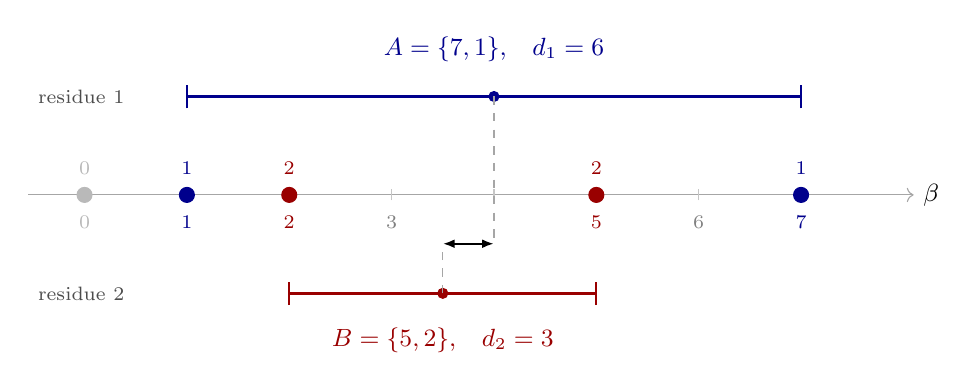
\begin{tikzpicture}[font=\small,x=1.3cm,y=1.0cm]
% --- the two intervals, well clear of the axis ---
\draw[blue!55!black,very thick] (1,1.25) -- (7,1.25);
\draw[blue!55!black,thick] (1,1.10) -- (1,1.40);
\draw[blue!55!black,thick] (7,1.10) -- (7,1.40);
\filldraw[blue!55!black] (4,1.25) circle (1.8pt);
\node[blue!55!black,above=9pt] at (4,1.25) {$A=\{7,1\}$,\quad $d_1=6$};
\draw[red!60!black,very thick] (2,-1.25) -- (5,-1.25);
\draw[red!60!black,thick] (2,-1.40) -- (2,-1.10);
\draw[red!60!black,thick] (5,-1.40) -- (5,-1.10);
\filldraw[red!60!black] (3.5,-1.25) circle (1.8pt);
\node[red!60!black,below=9pt] at (3.5,-1.25) {$B=\{5,2\}$,\quad $d_2=3$};
% --- the beta line ---
\draw[->,gray!70] (-0.55,0) -- (8.1,0) node[right,black]{$\beta$};
\foreach \b in {0,...,7} \draw[gray!45] (\b,-0.07) -- (\b,0.07);
\foreach \b in {3,6} \node[gray,font=\scriptsize,below=4pt] at (\b,0) {$\b$};
\foreach \b/\c/\r in {7/blue!55!black/1, 5/red!60!black/2, 2/red!60!black/2,
                      1/blue!55!black/1, 0/gray!55/0}
  {\filldraw[\c] (\b,0) circle (2.7pt);
   \node[\c,font=\scriptsize,below=4pt] at (\b,0) {$\b$};
   \node[\c,font=\scriptsize,above=4pt] at (\b,0) {$\r$};}
% --- the centres and their distance ---
\draw[gray!70,dashed] (4,1.25) -- (4,-0.62);
\draw[gray!70,dashed] (3.5,-1.25) -- (3.5,-0.62);
\draw[{Latex[length=1.5mm]}-{Latex[length=1.5mm]},thick] (3.5,-0.62) -- (4,-0.62);
\node[font=\scriptsize,gray!60!black,anchor=west] at (-0.55,1.25) {residue $1$};
\node[font=\scriptsize,gray!60!black,anchor=west] at (-0.55,-1.25) {residue $2$};
\end{tikzpicture}
\caption{The mechanism for $t=3$, $\lambda=(3,2)$: here $N=5$, $\beta=(7,5,2,1,0)$ with residues
$(1,2,2,1,0)$ modulo $3$, so no class is empty and two classes have size two. The three arguments of
\eqref{eq:main} are the two interval lengths and twice the distance between the interval centres;
the short double arrow marks that distance, here $\tfrac12$, so that $d_3=1$.}
\label{fig:intervals}
\end{figure}

\begin{example}
For $t=3$, $\lambda=(3,2)$ as in Figure \ref{fig:intervals}, $(d_1,d_2,d_3)=(6,3,1)$ and
\[
\Phi_3\bigl((3,2);z\bigr)=\varepsilon\,
\frac{\sinh(3\theta)\sinh(\theta/2)}{\sinh(3\theta/2)\sinh\theta}.
\]
For $t=3$, $\lambda=(3,1)$ the profile is the size-three one, $(d_1,d_2,d_3)=(3,3,6)$ and
$\Phi_3=\varepsilon\,\chi_2(z)$. For $t=4$, $\lambda=(1,1,1)$ we have $\beta=(6,5,4,2,1,0)$, the
class $3$ is empty and $\Phi_4=0$.
\end{example}

\subsection{The image of the map}
Theorem \ref{thm:main} sends every partition with at most $N$ rows to three integers, so the whole
family collapses onto a sparse subset of $\ZZ^3$. By Proposition \ref{prop:quotient} the first two
coordinates are multiples of $t$; the third is not a multiple of $t$ except in the size-three
profile, where $d_3=d_1+d_2$. Figure \ref{fig:image} shows the image for $t=3$ and $t=4$, coloured
by the number of partitions collapsing onto each point.

\begin{figure}[t]
\centering
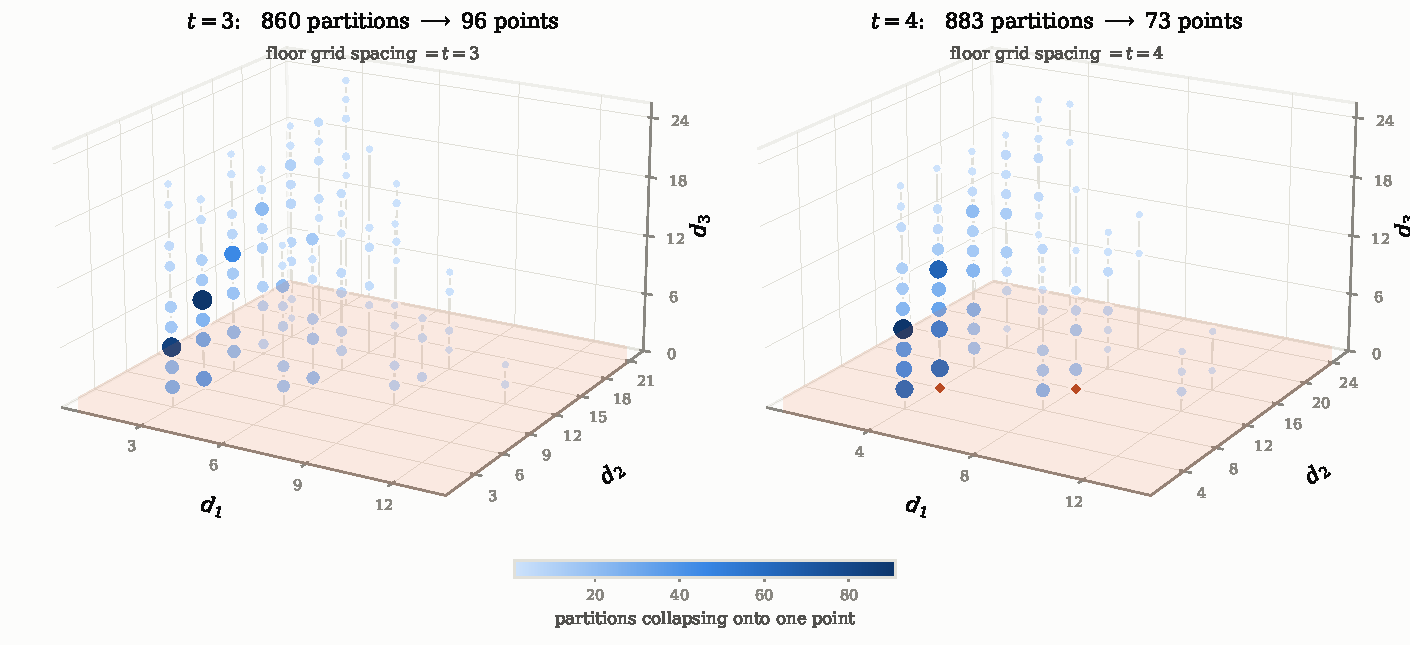
\includegraphics[width=\textwidth]{fig_image.pdf}
\caption{The image of $\lambda\mapsto(d_1,d_2,d_3)$ over all $\lambda$ with $|\lambda|\le20$ and at
most $t+2$ rows, for $t=3$ (left) and $t=4$ (right), taken \emph{up to the exchange of $d_1$ and
$d_2$}, under which \eqref{eq:main} is symmetric; without that identification, and with $A$ and $B$
in the order $r_A\le r_B$ of Theorem \ref{thm:main}, the two panels carry $126$ and $92$ points
rather than $96$ and $73$. The compression is the point of the picture: $860$
partitions land on $96$ triples on the left and $883$ on $73$ on the right, and colour and area give
the number of partitions mapping to each. The floor grid spacing is $t$, since $d_1,d_2\in t\ZZ$ by Proposition
\ref{prop:quotient}; the shaded plane $d_3=0$ is the concentric locus of Corollary \ref{cor:zero},
where $s_\lambda$ vanishes, so those shapes are not in the image and are drawn on the plane as
diamonds instead. The two panels are the two parities, which is the content of Proposition
\ref{rem:lattice}: the odd one carries no diamond, and can carry none; the even one carries two,
between them the images of $32$ partitions.}
\label{fig:image}
\end{figure}

Figure \ref{fig:image} is one half of the picture: it shows which triples occur, not what a triple
hides. Figure \ref{fig:fibres} is the other half. Over each cell of the $(d_1,d_2)$ floor it stands
the column of sizes $|\lambda|$ that land there, so a column is a set of partitions of different
sizes on which $\Phi_t$ takes one and the same value --- and the columns do not thin out as
$|\lambda|$ grows, since the values are confined to a lattice and the partitions are not. The most
visible one is the fibre of the empty partition: at $t=3$ the invariant $I_3=(3,3,2,+1)$ is shared by
$26$ partitions, of $19$ different sizes between $0$ and $20$, so $\Phi_3$ does not distinguish
$\varnothing$ from a shape of twenty boxes.

\begin{figure}[!ht]
\centering
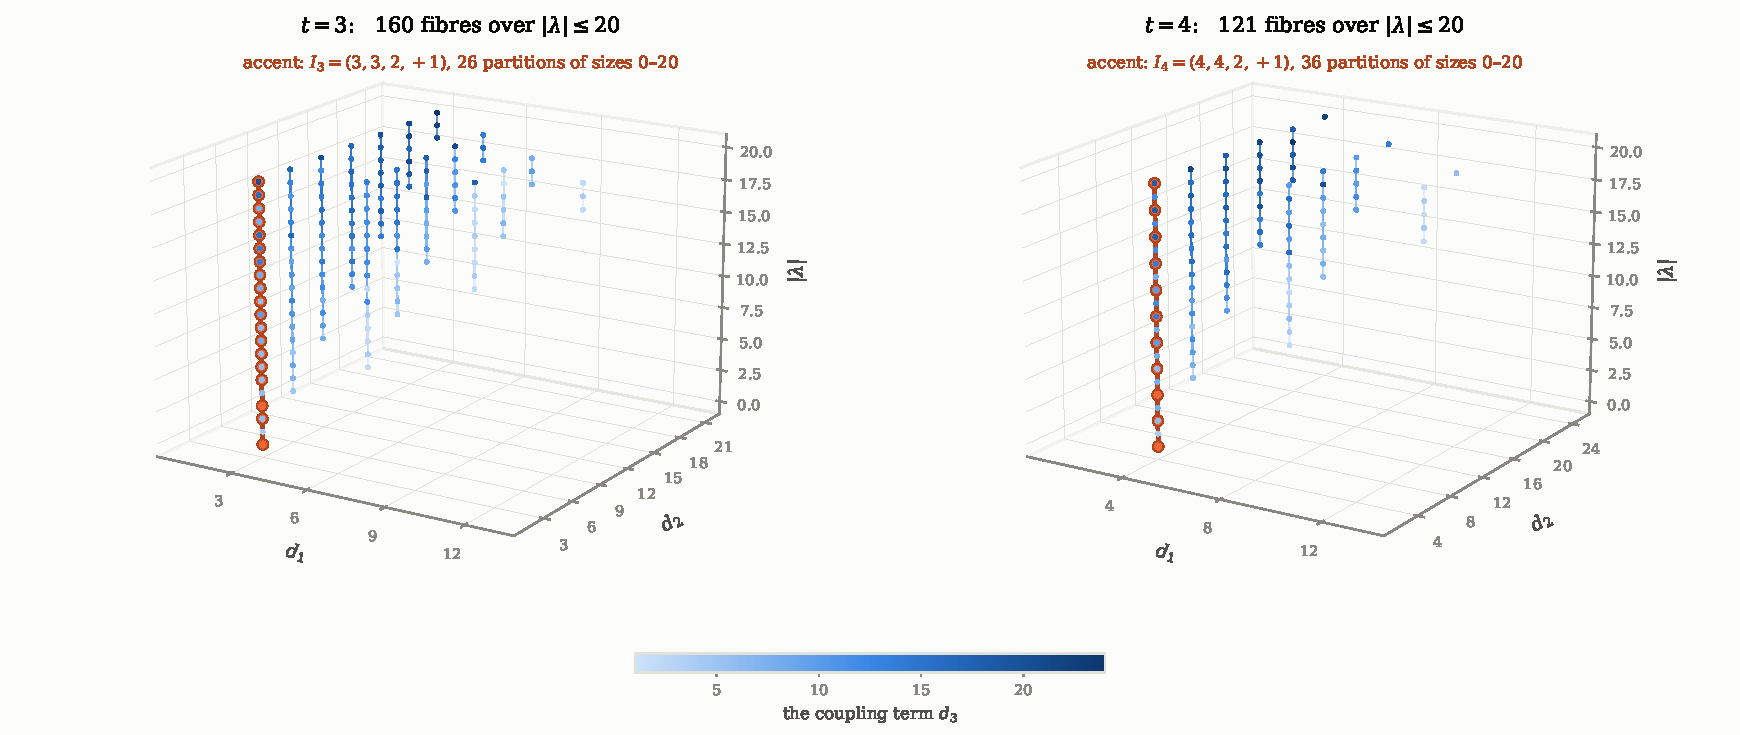
\includegraphics[width=\textwidth]{fig_fibres.pdf}
\caption{The fibres of the evaluation invariant \eqref{eq:invariant}, the complement of Figure
\ref{fig:image}: the same range $|\lambda|\le20$, with the coupling term moved to colour and the
size $|\lambda|$ on the vertical axis. A column is one fibre, so its height is the range of sizes
this alphabet cannot tell apart; the floor ticks are the lattice $t\ZZ$ of Proposition
\ref{prop:quotient}, and only the half $d_1\le d_2$ is occupied because the triple is taken up to the
exchange, as in Figure \ref{fig:image}. That every marker of a column carries the same value is
computed and not assumed: over the $860$ partitions on the left and the $883$ on the right the
bialternant is constant on each fibre to $10^{-37}$. The accent column is the fibre of
$\lambda=\varnothing$.}
\label{fig:fibres}
\end{figure}

Figure \ref{fig:fibres} makes one thing about \eqref{eq:invariant} precise: $I_t$ is complete but
not minimal. The numerator of \eqref{eq:main} is symmetric in $d_1,d_2,d_3$, so the value sees only the multiset
$\{d_1,d_2,d_3\}$ together with the sign, and that is a real reduction --- over $t=4$ and
$|\lambda|\le20$ the $121$ invariants take only $110$ values, while at $t=3$ in the same range the
two counts agree. In the same range no two distinct multisets share a value, so the minimal invariant
of this evaluation is the pair (multiset, sign); we keep the ordered form in \eqref{eq:invariant}
because $d_3$ is the coordinate the reciprocal pair contributes and the other two are not, and
Corollary \ref{cor:fibregf} describes the fibres of either, since the two differ by a symmetry of
the numerator and not by anything the lattice sees.

\begin{proposition}[a shorter form of the sign]\label{rem:sign}
Let the residue profile be non-degenerate and $a_1+a_2\ne b_1+b_2$, and order the two distinguished
classes so that $r_A\le r_B$. Then
\begin{equation}\label{eq:shortsign}
\boxed{\;\;\varepsilon_\lambda\;=\;(-1)^{\lfloor t/2\rfloor}\,\sgn(\sigma)\,(-1)^{\,r_A+r_B}\,
\sgn\bigl(a_1+a_2-b_1-b_2\bigr)\;\;}
\end{equation}
where $\sigma$ is the permutation of \S\ref{sec:background}.
\end{proposition}

\begin{proof}
Let $w$ be the residue word of $\beta(\lambda)$ read in increasing column order. Since $\beta$
decreases with the column index, grouping the parts by class with the values decreasing inside each
class is the stable sort of $w$, so $\sgn(\sigma)=(-1)^{\inv(w)}$. Both sides of
\eqref{eq:shortsign} carry the factor $\sgn(a_1+a_2-b_1-b_2)$, and
$\sgn(a_1-b_1)=(-1)^{[a_1<b_1]}$, so by \eqref{eq:sign} the assertion is equivalent to
\begin{equation}\label{eq:signparity}
j_{A_1}+j_{B_1}+\inv(w)+\inv(b_S)+[a_1<b_1]\;\equiv\;
\Bigl\lfloor\tfrac t2\Bigr\rfloor+t+\binom{N+1}{2}+r_A+r_B \pmod 2 .
\end{equation}

We use one parity count. Let $u$ be a word, $p$ a position, $c=u_p$, and let $I(p)$ be the number of
inversions of $u$ in which $p$ takes part; write $\nu_{<c}$ for the number of letters of $u$ strictly
below $c$ and $e_p$ for the number of occurrences of $c$ strictly before $p$. Putting
$x=\#\{j<p:u_j>c\}$, the positions before $p$ split as $p-1=x+e_p+\#\{j<p:u_j<c\}$ and the letters
below $c$ split as $\nu_{<c}=\#\{j<p:u_j<c\}+\#\{j>p:u_j<c\}$, whence
\begin{equation}\label{eq:parity}
I(p)\;=\;x+\#\{j>p:u_j<c\}\;=\;2x+e_p+\nu_{<c}-(p-1)\;\equiv\;(p-1)+\nu_{<c}+e_p \pmod 2 .
\end{equation}
Since $b_S$ is $w$ with the letters at the positions $j_{A_1}$ and $j_{B_1}$ deleted,
\[
\inv(w)-\inv(b_S)=I(j_{A_1})+I(j_{B_1})
-\bigl[\,\{j_{A_1},j_{B_1}\}\ \text{is an inversion of }w\,\bigr],
\]
and $\inv(w)+\inv(b_S)\equiv\inv(w)-\inv(b_S)$, so \eqref{eq:parity} computes the left-hand side of
\eqref{eq:signparity}.

In the two-class profile $r_A<r_B$, and $w$ carries $r_A$ twice, $r_B$ twice and every other residue
once. Because $\beta$ decreases with the column index, $a_1>a_2$ puts $j_{A_1}$ at the \emph{first}
occurrence of $r_A$, so $e=0$ there, and likewise at $j_{B_1}$. The letters below $r_A$ are one copy
of each of $0,\dots,r_A-1$, so $\nu_{<r_A}=r_A$; those below $r_B$ are the same together with the
second copy of $r_A$, so $\nu_{<r_B}=r_B+1$. The two positions form an inversion exactly when the
larger letter comes first, that is when $j_{B_1}<j_{A_1}$, that is when $a_1<b_1$. Hence
\[
\inv(w)-\inv(b_S)\;\equiv\;(j_{A_1}-1+r_A)+(j_{B_1}-1+r_B+1)+[a_1<b_1]
\;\equiv\;j_{A_1}+j_{B_1}+r_A+r_B+1+[a_1<b_1],
\]
and substituting this in \eqref{eq:signparity} cancels the columns and $[a_1<b_1]$ in pairs, leaving
$\lfloor t/2\rfloor+t+\binom{N+1}{2}\equiv1$.

In the size-three profile $r_A=r_B=:r$ and the class $\{p>q>p'\}$ sits at columns $j_1<j_2<j_3$ with
$A=\{p,q\}$ and $B=\{q,p'\}$, so $j_{A_1}=j_1$ and $j_{B_1}=j_2$ carry the same letter $r$, with
$e=0$ and $e=1$ respectively and $\nu_{<r}=r$ in both; two equal letters are not an inversion, and
$a_1>b_1$. So $\inv(w)-\inv(b_S)\equiv j_1+j_2+1$, which is the displayed expression again because
$r_A+r_B=2r$ and $[a_1<b_1]=0$, and \eqref{eq:signparity} reduces to the same congruence.

Finally $N=t+2$, so that congruence reads $\lfloor t/2\rfloor+t+\binom{t+3}{2}\equiv1$: for $t=2m$
its three terms are $m$, $0$ and $m+1$, and for $t=2m+1$ they are $m$, $1$ and $m$. Both sums are
odd, and the identity holds for every $t\ge2$.
\end{proof}

The ordering by residue is not a convenience, and it is worth saying why. Exchanging the two blocks
negates the sign $\kappa_{11}$ of Lemma \ref{lem:L4} --- through its $\sgn(a_1-b_1)$ factor --- and negates
$\sgn(a_1+a_2-b_1-b_2)$ as well, so it leaves $\varepsilon_\lambda$, which is their product,
invariant; as it must, since $\varepsilon_\lambda$ is attached to $\lambda$. The right-hand side
above is \emph{not} invariant: $(-1)^{r_A+r_B}$ is symmetric, so only its last factor changes sign.
Without a rule fixing which block is $A$, the right-hand side is therefore not a function of
$\lambda$ at all. The hypothesis enters the proof at one point and one only: it is what makes
$\nu_{<r_A}=r_A$ and $\nu_{<r_B}=r_B+1$ rather than the other way round, and dropping it exchanges
those two counts and breaks \eqref{eq:signparity}.

Read the other way round, \eqref{eq:shortsign} says that $\Phi_t$ is a function of a small
combinatorial datum and of nothing else, and it says so for every $t$ rather than over a range: by
Theorem \ref{thm:main} the triple $(d_1,d_2,d_3)$ determines $\Phi_t$ up to sign, and adjoining
$\sgn(\sigma)$, the ordered pair $r_A\le r_B$ and the \emph{orientation}
$\sgn(a_1+a_2-b_1-b_2)$ of $d_3$ determines it outright. The shape of $\lambda$ enters nowhere else.
The orientation is not optional, and that part remains a check rather than a proof: over $t\le6$ and
$|\lambda|\le14$, putting $\sgn(a_1-b_1)$ in its place leaves collisions at $t=2$.

%======================================================================
\section{Proof of Theorem \ref{thm:main}}\label{sec:proof}

The proof uses the Vandermonde determinant, the Laplace expansion, and one cancellation lemma. We
give the steps separately so that a reader checking the ancillary scripts can localise any
disagreement.

What the argument really does is classify rather than compute. Expanding along the $t$ frozen rows
leaves one term for each way of choosing which two columns are \emph{not} frozen, and the excess-two
count says every such choice falls into exactly one of three combinatorial types: none survives
(a residue class is empty), four survive (two classes of size two), or three do (one class of size
three). Everything after that is bookkeeping inside a type, and Lemma \ref{lem:L5} shows the last two
types are one statement seen twice.

\begin{lemma}\label{lem:L1}
Let $S$ be a set of $t$ columns and $M_S=\det(\zeta^{k\beta_j})_{0\le k<t,\,j\in S}$. Then $M_S=0$
unless the residues $\{\beta_j\bmod t:j\in S\}$ are pairwise distinct, in which case
$M_S=(-1)^{\inv(b_S)}V$.
\end{lemma}

\begin{proof}
Since $\zeta^{k\beta_j}=(\zeta^{\beta_j})^k$, the matrix is a Vandermonde matrix in the values
$y_j=\zeta^{\beta_j}$, whose determinant is $\prod_{j<j'}(y_{j'}-y_j)$. The value $y_j$ depends on
$\beta_j$ only modulo $t$, so two columns of $S$ sharing a residue make the determinant vanish. If
the residues are pairwise distinct then $|S|=t$ forces $\{y_j\}_{j\in S}=\zt$ as a set, and the
Vandermonde determinant is alternating in its arguments, so it equals $V$ times the sign of the
permutation sorting $b_S$ increasingly, which is $(-1)^{\inv(b_S)}$.
\end{proof}

\begin{lemma}\label{lem:L2}
$\det\bigl(x_i^{N-j}\bigr)_{i,j=1}^{N}
=(-1)^{\binom t2}\,V\,(z^t-1)(z^{-t}-1)(z-z^{-1})$ for the alphabet
$x=(1,\zeta,\dots,\zeta^{t-1},z,z^{-1})$ in that order.
\end{lemma}

\begin{proof}
The determinant is $\prod_{i<i'}(x_i-x_{i'})$. Pairs inside $\zt$ contribute
$\prod_{k<k'}(\zeta^k-\zeta^{k'})=(-1)^{\binom t2}V$; pairs $(\zeta^k,z)$ contribute
$\prod_k(\zeta^k-z)=(-1)^t(z^t-1)$ and pairs $(\zeta^k,z^{-1})$ contribute $(-1)^t(z^{-t}-1)$; the
last pair contributes $z-z^{-1}$. The two factors $(-1)^t$ cancel.
\end{proof}

\begin{lemma}\label{lem:L3}
Let $\mathcal U$ be the set of pairs $U=\{j_1<j_2\}$ of columns whose complement $S_U$ carries all
$t$ residues. Then
\[
\Phi_t(\lambda;z)=\frac{(-1)^{\,t+\binom{N+1}{2}}}{(z^t-1)(z^{-t}-1)(z-z^{-1})}
\sum_{U\in\mathcal U}(-1)^{\,j_1+j_2+\inv(b_{S_U})}\,f(\beta_{j_1}-\beta_{j_2}).
\]
\end{lemma}

\begin{proof}
Expanding the numerator by Laplace along the first $t$ rows,
\[
\det\bigl(x_i^{\beta_j}\bigr)=\sum_{|S|=t}(-1)^{\binom{t+1}{2}+\sum_{j\in S}j}\,M_S\,C_{S^c},
\]
where for $S^c=\{j_1<j_2\}$ the complementary $2\times2$ minor is
$z^{\beta_{j_1}-\beta_{j_2}}-z^{-(\beta_{j_1}-\beta_{j_2})}=f(\beta_{j_1}-\beta_{j_2})$. By Lemma
\ref{lem:L1} only $S$ with pairwise distinct residues contribute. Writing
$\sum_{j\in S}j=\binom{N+1}{2}-j_1-j_2$ and dividing by Lemma \ref{lem:L2}, the factors $V$ cancel
and $(-1)^{\binom{t+1}{2}-\binom{t}{2}}=(-1)^t$.
\end{proof}

If some $n_i=0$ then no $S$ of size $t$ carries all residues, $\mathcal U=\varnothing$, and
$\Phi_t=0$: this is Theorem \ref{thm:main}(i). Otherwise all $n_i\ge1$ and by \eqref{eq:excess}
either two classes have size two, in which case $S_U$ must drop one element of each and
$|\mathcal U|=4$, or one class has size three, in which case $S_U$ drops two of the three and
$|\mathcal U|=3$.

\begin{lemma}[the column move]\label{lem:L4}
Let $A$ and $B$ be distinct classes of size two, at columns $j_{A_1}<j_{A_2}$ and
$j_{B_1}<j_{B_2}$. For $i,j\in\{1,2\}$ let $U_{ij}$ consist of the column of $a_i$ and the column of
$b_j$, and set $\kappa_{ij}=(-1)^{\,j_{A_i}+j_{B_j}+\inv(b_{S_{U_{ij}}})}\sgn(a_i-b_j)$, so that
the $U_{ij}$ term of Lemma \ref{lem:L3} equals $\kappa_{ij}f(a_i-b_j)$. Then
$\kappa_{ij}=\kappa_{11}(-1)^{i-1}(-1)^{j-1}$.
\end{lemma}

\begin{proof}
Fix $j$ and compare $i=1$ with $i=2$. The sets $S_{U_{1j}}$ and $S_{U_{2j}}$ differ only in that the
first contains the column $j_{A_2}$ and the second the column $j_{A_1}$, and the letter carried is
the residue $r_A$ in both. Passing from one word to the other moves that letter across exactly the
kept columns strictly between $j_{A_1}$ and $j_{A_2}$, and none of those letters equals $r_A$
because the class $A$ has only two elements; each crossing changes the parity of $\inv$. Hence
\[
(-1)^{\inv(b_{S_{U_{1j}}})-\inv(b_{S_{U_{2j}}})}
=(-1)^{(j_{A_2}-j_{A_1}-1)-[\,a_2<b_j<a_1\,]},
\]
using that $\beta$ is strictly decreasing in the column index, so that $j_{B_j}$ lies strictly
between $j_{A_1}$ and $j_{A_2}$ exactly when $a_2<b_j<a_1$. Multiplying by the Laplace factor
$(-1)^{j_{A_1}+j_{A_2}}$,
\[
\frac{\kappa_{1j}}{\kappa_{2j}}
=(-1)^{2j_{A_2}-1}(-1)^{[\,a_2<b_j<a_1\,]}\sgn(a_1-b_j)\sgn(a_2-b_j)=-1,
\]
because $\sgn(a_1-b_j)\sgn(a_2-b_j)=-1$ exactly when $b_j$ lies between $a_2$ and $a_1$. Exchanging
the roles of $A$ and $B$ gives $\kappa_{i1}/\kappa_{i2}=-1$.
\end{proof}

\begin{lemma}\label{lem:L5}
For all $c,p,q$ and all $u,v$,
\begin{align*}
\text{\rm(a)}&\quad \sum_{\epsilon,\eta\in\{\pm1\}}\epsilon\eta\,f(c+\epsilon p+\eta q)=f(c)f(p)f(q),\\
\text{\rm(b)}&\quad f(2u)-f(2u+2v)+f(2v)=-f(u)f(v)f(u+v).
\end{align*}
\end{lemma}

\begin{proof}
For (a), $\sum_{\epsilon,\eta}\epsilon\eta\,z^{c+\epsilon p+\eta q}
=z^{c}\bigl(\sum_\epsilon\epsilon z^{\epsilon p}\bigr)\bigl(\sum_\eta\eta z^{\eta q}\bigr)
=z^{c}f(p)f(q)$, and the same computation for the negative exponents gives
$z^{-c}(-f(p))(-f(q))$; subtract. For (b), put $s=z^u$, $w=z^v$ and expand
$(s-s^{-1})(w-w^{-1})(sw-s^{-1}w^{-1})$: the eight terms recombine as
$(s^2w^2-s^{-2}w^{-2})-(s^2-s^{-2})-(w^2-w^{-2})=f(2u+2v)-f(2u)-f(2v)$.
\end{proof}

\begin{proof}[Proof of Theorem \ref{thm:main}]
In the two-class profile, Lemmas \ref{lem:L3} and \ref{lem:L4} give
\[
\sum_{U\in\mathcal U}(\cdots)=\kappa_{11}\sum_{i,j}(-1)^{i-1}(-1)^{j-1}f(a_i-b_j).
\]
Writing $a_i=\alpha+\epsilon_ip$ and $b_j=\gamma+\eta_jq$ with $p=d_1/2$, $q=d_2/2$ and
$\epsilon=\eta=(+1,-1)$, we have $a_i-b_j=c+\epsilon_ip-\eta_jq$ with $c=\alpha-\gamma$. Replacing
$\eta$ by $-\eta$ turns the sum into $-\sum_{\epsilon,\eta}\epsilon\eta f(c+\epsilon p+\eta q)$,
which is $-f(c)f(p)f(q)$ by Lemma \ref{lem:L5}(a). Since
$(z^t-1)(z^{-t}-1)=2-z^t-z^{-t}=-f(t/2)^2$ and $z-z^{-1}=f(1)$, the two minus signs cancel, and
substituting $f(u)=2\sinh(u\theta)$ the numerical factors cancel and
$\sinh(c\theta)=\sgn(c)\sinh(d_3\theta/2)$, giving \eqref{eq:main} with
$\varepsilon_\lambda=(-1)^{\,t+\binom{N+1}{2}}\kappa_{11}\sgn(a_1+a_2-b_1-b_2)$, which is
\eqref{eq:sign} by the definition of $\kappa_{11}$ in Lemma \ref{lem:L4}.

For the size-three profile $\{p>q>r\}$ at columns $j_1<j_2<j_3$ the same column-move argument
applies, again because no letter strictly between two of these columns carries the class residue,
and gives alternating signs $(\varsigma,-\varsigma,\varsigma)$ for the three terms $f(p-q)$,
$f(p-r)$, $f(q-r)$. By Lemma \ref{lem:L5}(b) with $u=(p-q)/2$, $v=(q-r)/2$ the sum is
$-\varsigma f(u)f(v)f(u+v)$, which is the two-class formula for $A=\{p,q\}$, $B=\{q,r\}$ with
$\varsigma=\kappa_{11}$. Equivalently, the missing fourth selection of the two-class profile would
drop $q$ twice and its term carries $f(0)=0$, so the two profiles are one statement.
\end{proof}

All the statements of this paper were also checked numerically; the counts are collected once, in
\S\ref{sec:verif}, rather than repeated as they arise.

%======================================================================
\section{Independence on the reciprocal locus}\label{sec:independence}

Specializing \eqref{eq:AK53} as in \S\ref{sec:background} gives: for $\ell(\lambda)\le2$,
$s_\lambda(z,\zb,\zt)=s_\lambda(z,\zb)$ if and only if $\lambda=\core_t(\lambda)$. Theorem
\ref{thm:main} evaluates the left-hand side for every $\lambda$, and comparing the two shows that on
the reciprocal locus the criterion acquires further solutions --- exactly one family.

We first isolate when $\Phi_t$ degenerates to a single character. Recall
$\chi_k(z)=(z^{k+1}-z^{-k-1})/(z-z^{-1})$.

\begin{lemma}\label{lem:single}
$\Phi_t(\lambda;z)=\pm\chi_k(z)$ for some $k\ge0$ if and only if the multiset $\{d_1,d_2,d_3\}$
contains $t$ at least twice, and in that case the remaining entry equals $2(k+1)$.
\end{lemma}

\begin{proof}
Put $u=z^{1/2}$, so that $2\sinh(d_i\theta/2)=u^{d_i}-u^{-d_i}$, $2\sinh(t\theta/2)=u^{t}-u^{-t}$ and
$2\sinh\theta=u^{2}-u^{-2}$; all exponents are integers. By \eqref{eq:main}, the asserted equality is
\[
\prod_{i=1}^{3}\bigl(u^{d_i}-u^{-d_i}\bigr)
=\pm\bigl(u^{t}-u^{-t}\bigr)^{2}\bigl(u^{2k+2}-u^{-2k-2}\bigr).
\]
Using $u^{n}-u^{-n}=u^{-n}(u^{2n}-1)$ on each factor and comparing the monomial prefactors gives
$d_1+d_2+d_3=2t+2(k+1)$ together with
\[
\prod_{i=1}^{3}\bigl(u^{2d_i}-1\bigr)=\pm\bigl(u^{2t}-1\bigr)^{2}\bigl(u^{4(k+1)}-1\bigr),
\]
and evaluating at $u=0$ fixes the sign to $+$. Now $u^{2n}-1=\prod_{m\mid 2n}\Phi_m(u)$ with
$\Phi_m$ the cyclotomic polynomials, which are irreducible and pairwise distinct, so by unique
factorization in $\ZZ[u]$ the two sides have the same multiset of cyclotomic factors. On the left
that multiset is $\biguplus_i\{m:m\mid 2d_i\}$ and on the right it is
$2\times\{m:m\mid 2t\}\uplus\{m:m\mid 4(k+1)\}$. Its largest element is $\max_i 2d_i$ on the left and
$\max(2t,4(k+1))$ on the right; deleting the divisor set of that maximum from both sides and
repeating twice more yields
\[
\{2d_1,2d_2,2d_3\}=\{2t,\,2t,\,4(k+1)\}
\]
as multisets, which is the assertion. The converse is the same computation read backwards.
\end{proof}

\begin{theorem}\label{thm:extra}
Let $\ell(\lambda)\le2$. Then $\Phi_t(\lambda;z)=\pm s_\lambda(z,\zb)$ if and only if either
$\lambda=\core_t(\lambda)$, or
\begin{equation}\label{eq:extra}
t\ \text{is even}\quad\text{and}\quad \lambda=\Bigl(\lambda_2+\tfrac{3t}{2}-1,\ \lambda_2\Bigr)
\quad\text{with}\quad \tfrac t2\le\lambda_2\le t-1 .
\end{equation}
In the second case $\{d_1,d_2,d_3\}=\{3t,t,t\}$, while $\core_t(\lambda)=\bigl(\tfrac t2-1+j,j\bigr)$
and $\quot_t(\lambda)$ has the single nonempty component $(2)$, in slot $j=\lambda_2-\tfrac t2$.
\end{theorem}

Figure \ref{fig:locus} is the statement computed rather than asserted: both families are plotted
over a range of $t$, and the odd $t$ where \eqref{eq:extra} cannot occur is drawn as the control.

\begin{figure}[!ht]
\centering

\includegraphics[width=\textwidth]{fig_locus.pdf}
\caption{Theorem \ref{thm:extra}, computed rather than asserted. For every two-row $\lambda$ in
range, both sides of $\Phi_t(\lambda;z)=\pm s_\lambda(z,\zb)$ were evaluated; the partitions where
they agree are plotted and coloured by family. Circles are the $t$-cores, the solutions already
described by \eqref{eq:AK53}; triangles are the extra family \eqref{eq:extra}, which the reciprocal
specialization creates. The odd case $t=3$ is the control: by Theorem \ref{thm:extra} no extra
solution can exist there, and none is found.}
\label{fig:locus}
\end{figure}

\begin{proof}
Since $\ell(\lambda)\le 2$ and $N=t+2$, the beta set is
$\beta(\lambda)=\bigl(A'+t,\;B'+t,\;t-1,t-2,\dots,1,0\bigr)$ where
\[
A':=\lambda_1+1,\qquad B':=\lambda_2,\qquad A'>B'\ge0 .
\]
The block $\{0,1,\dots,t-1\}$ meets every residue class exactly once, so no class is empty and the
two large parts decide the profile. Write $A'=t\alpha+\rho_A$ and $B'=t\gamma+\rho_B$ with
$0\le\rho_A,\rho_B\le t-1$. As $s_\lambda(z,\zb)=\chi_{\lambda_1-\lambda_2}(z)$, Lemma
\ref{lem:single} says that the assertion holds precisely when $\{d_1,d_2,d_3\}$ contains $t$ twice
and the third entry is $2(\lambda_1-\lambda_2+1)=2(A'-B')$.

\emph{Case $\rho_A=\rho_B=:\rho$.} One class has size three, namely $\{A'+t,B'+t,\rho\}$, and by
Theorem \ref{thm:main} the three arguments are
$d_1=A'-B'$, $d_2=B'+t-\rho=t(\gamma+1)$, $d_3=A'+t-\rho=t(\alpha+1)$. Here $t\mid A'-B'$, say
$A'-B'=ts$ with $s\ge1$. The pair $d_2=d_3=t$ forces $\alpha=\gamma=0$, hence $A'=B'$, excluded.
The pair $d_1=d_3=t$ forces $s=1$ and $\alpha=0$, hence $A'<t$ and $A'=B'+t\ge t$, excluded. The pair
$d_1=d_2=t$ forces $s=1$ and $\gamma=0$, i.e. $A'=B'+t$ with $B'<t$; then $\alpha=1$ and the third
entry is $d_3=2t=2(A'-B')$, as required. So this case contributes exactly the $\lambda$ with
$A'=B'+t$, $B'<t$.

\emph{Case $\rho_A\ne\rho_B$.} Two classes have size two, namely $\{A'+t,\rho_A\}$ and
$\{B'+t,\rho_B\}$, and the three arguments are
\[
d_A=t(\alpha+1),\qquad d_B=t(\gamma+1),\qquad
d_3=\bigl|\,t(\alpha-\gamma)+2(\rho_A-\rho_B)\,\bigr| .
\]
If $d_A=d_B=t$ then $\alpha=\gamma=0$, so $A',B'<t$ and $d_3=2|\rho_A-\rho_B|=2(A'-B')$
automatically: every such $\lambda$ is a solution. Otherwise exactly one of $d_A,d_B$ equals $t$ and
$d_3=t$. If $\alpha=0$ and $\gamma\ge1$ then $|-t\gamma+2(\rho_A-\rho_B)|=t$ with
$|\rho_A-\rho_B|\le t-1$ forces $\gamma=2$ and $\rho_A-\rho_B=t/2$; but then
$\lambda_1=A'-1=\rho_A-1<t$ while $\lambda_2=B'\ge2t$, contradicting $\lambda_1\ge\lambda_2$. If
$\gamma=0$ and $\alpha\ge1$ then $|t\alpha+2(\rho_A-\rho_B)|=t$ forces, for $\alpha=1$,
$\rho_A=\rho_B$ (excluded), and for $\alpha=2$,
\[
\rho_B-\rho_A=\tfrac t2,
\]
which requires $t$ even; $\alpha\ge3$ gives $|2(\rho_A-\rho_B)|\ge2t$, impossible. So $A'=2t+\rho_A$,
$B'=\rho_B=\rho_A+\tfrac t2$, whence
\[
\lambda_1=2t+\rho_A-1,\qquad \lambda_2=\rho_A+\tfrac t2,\qquad
\lambda_1-\lambda_2=\tfrac{3t}{2}-1,
\]
and $\rho_B\le t-1$ gives $0\le\rho_A\le\tfrac t2-1$, i.e. $\tfrac t2\le\lambda_2\le t-1$. The
remaining entry is $d_A=t(\alpha+1)=3t=2(\lambda_1-\lambda_2+1)$, as required. This is
\eqref{eq:extra}.

It remains to identify the solutions collected in the first case of each analysis with the
$t$-cores. For $\ell(\lambda)\le2$ the beta set in two slots is $(A',B')$, and $\lambda$ is a
$t$-core if and only if neither beta number can be lowered by $t$ into an unoccupied nonnegative
position, i.e. if and only if $B'<t$ and either $A'<t$ or $A'=B'+t$. These are exactly the two
families found above. Finally, in case \eqref{eq:extra} the class $\rho_A$ carries
$\{2t+\rho_A+t,\rho_A\}$, so its quotient component is $(2)$, every other component is empty, and
the core is as stated.
\end{proof}


\begin{remark}\label{rem:why}
Theorem \ref{thm:extra} is stated up to sign because that is what Lemma \ref{lem:single} controls;
over two-row shapes with $t\le8$ the sign is $+1$ at every solution, so there the equality holds on
the nose.

The extra family belongs to the specialization rather than to the alphabet. The step is
\cite[Lemma 5.2]{AK25}, on which \cite[Theorem 5.3]{AK25} rests: it reduces the independence to the
vanishing of $s_{\lambda/\mu}$ at the twisted alphabet for all $\mu\subsetneq\lambda$, and the
reduction uses the linear independence of the universal characters $f_\mu$ in the free variables. On the reciprocal locus $s_\mu(z,\zb)=\chi_{\mu_1-\mu_2}(z)$
depends only on $\mu_1-\mu_2$, so $s_{(1)}$, $s_{(2,1)}$ and $s_{(3,2)}$ agree there and that
independence is not available; Theorem \ref{thm:extra} measures the difference. A control confirms
the reading: for $\lambda=(3,1)$ and $t=2$ one has $s_\lambda(\zt,z,\zb)=s_\lambda(z,\zb)$, while
$s_\lambda(\zt,x,y)\ne s_\lambda(x,y)$ for free $x,y$.
\end{remark}

So the criterion does not survive the specialization unchanged, and what it acquires is small and
nameable: one family, for two-row shapes, indexed by an order-two element of the residue lattice and
classified by its core and quotient. The extra solutions belong to the reciprocal locus, not to the
alphabet --- they exist because a specialization has removed a linear independence the original
argument used, and that missing step is exactly what Theorem \ref{thm:extra} measures.

%======================================================================
\section{An enumeration in which a parameter survives}\label{sec:enum}

Expanding $s_\lambda$ over semistandard tableaux turns Theorem \ref{thm:main} into a product formula
for a weighted count. Let $m_k(T)$ be the number of entries equal to $k$ in $T$.

\begin{corollary}\label{cor:enum}
Expanding $s_\lambda$ over semistandard tableaux and applying Theorem \ref{thm:main}: for every
$t\ge2$ and every $\lambda\in\PP_{t+2}$,
\[
\sum_{T\in\mathrm{SSYT}(\lambda,\,t+2)}
\zeta^{\,\sum_{k=1}^{t}(k-1)m_k(T)}\;z^{\,m_{t+1}(T)-m_{t+2}(T)}
\;=\;\varepsilon_\lambda\,
\frac{\sinh(d_1\theta/2)\sinh(d_2\theta/2)\sinh(d_3\theta/2)}{\sinh^2(t\theta/2)\sinh\theta}.
\]
\end{corollary}

For $t=2$ the weight is $(-1)^{m_2(T)}$, and if $\lambda=(c^r)$ is rectangular then
$\mathrm{SSYT}(\lambda,4)$ is in bijection with plane partitions in an $r\times(4-r)\times c$ box,
equivalently with lozenge tilings of a hexagon. Corollary \ref{cor:enum} is then a
$(-1)$-enumeration of those objects \emph{refined by a free parameter} $z$, which records the
difference between the numbers of entries $3$ and $4$. Setting $z=1$ recovers the plain signed
count, which by \eqref{eq:main} equals $\pm d_1d_2d_3/(2t^2)$: for $r=2$, $c=2$ it is $4$; for
$r=2$, $c=4$ it is $9$; for $r=3$, $c=3$ it is $-6$.

\begin{example}\label{ex:boxes}
Taking $\lambda=(c^{\,r})$ with $1\le r\le4$ and $t=2$, the shape has at most four rows, the tableaux
are the plane partitions in an $r\times(4-r)\times c$ box, and the closed form gives the signed
counts of Figure \ref{fig:signed}. Reading it off:
\[
\begin{array}{ll}
1\times3\times c: & \bigl\lfloor (c+2)^2/4\bigr\rfloor,\\[2pt]
2\times2\times c: & (c/2+1)^2 \text{ for } c \text{ even},\qquad 0 \text{ for } c \text{ odd},\\[2pt]
3\times1\times c: & (-1)^c\bigl\lfloor (c+2)^2/4\bigr\rfloor,\\[2pt]
4\times0\times c: & (-1)^c .
\end{array}
\]
The third row is the transpose of the first, which is why the magnitudes agree; the fourth is the
degenerate box, where $s_{(c^4)}(x)=(x_1x_2x_3x_4)^c$ and the alphabet has determinant $-1$. We do
not claim these particular counts as new --- the boxes are small and the sign here is the
specialization $x_2=-1$, not the complementation sign of Kuperberg's $(-1)$-enumerations --- and we
record them only to show what the theorem produces. What does appear to be new is that each of them
is the $z\mapsto1$ value of a one-parameter refinement with the same product formula.
\end{example}

The perfect squares in Example \ref{ex:boxes} are not an accident of small cases: they are what the
interval reading of \S\ref{sec:intervals} says a rectangle must produce.

\begin{proposition}\label{prop:rect}
Let $t=2$ and $\lambda=(c^{\,r})$ with $1\le r\le4$. Then one of $d_1,d_2,d_3$ equals $2$, and:
\begin{enumerate}
\item[\rm(i)] if $r=4$, all three equal $2$ for \emph{every} $c$ and the count is $(-1)^c$; this is
the full rectangle, where $s_{(c^4)}(x)=(x_1x_2x_3x_4)^{c}$ collapses to a monomial and the alphabet
contributes only its determinant;
\item[\rm(ii)] if $r\le3$ and $c$ is even, the other two are both equal to $c+2$, so the two
intervals have the \emph{same length} and the signed count is the perfect square
$\bigl(\tfrac{c+2}{2}\bigr)^2$;
\item[\rm(iii)] if $c$ is odd and $r=2$, the two intervals are \emph{concentric} and the count is $0$;
\item[\rm(iv)] if $c$ is odd and $r\in\{1,3\}$, the other two are $c+1$ and $c+3$, and the count is
$\pm\tfrac{(c+1)(c+3)}{4}=\pm\bigl\lfloor\tfrac{(c+2)^2}{4}\bigr\rfloor$.
\end{enumerate}
Case {\rm(i)} is not a degeneration of the interval triple but a collapse of the shape itself, and it
is the only case in which the parity of $c$ plays no role.
\end{proposition}

\begin{proof}
For $\lambda=(c^{\,r})$ the beta set consists of two blocks of consecutive integers, namely
$c+3,c+2,\dots,c+4-r$ and $3-r,2-r,\dots,0$; residues alternate along each block, which is what
forces the coincidences. Explicitly, for $r=1,2,3,4$ the beta set is $(c+3,2,1,0)$, $(c+3,c+2,1,0)$,
$(c+3,c+2,c+1,0)$ and $(c+3,c+2,c+1,c)$. Splitting each by parity gives, for $c$ even,
\[
\{c{+}3,1\},\{2,0\};\qquad \{c{+}3,1\},\{c{+}2,0\};\qquad \{c{+}3,c{+}1\},\{c{+}2,0\};\qquad
\{c{+}3,c{+}1\},\{c{+}2,c\},
\]
whence $(d_1,d_2,d_3)$ equals $(c{+}2,2,c{+}2)$, $(c{+}2,c{+}2,2)$, $(2,c{+}2,c{+}2)$ and
$(2,2,2)$ respectively; in each case the product over $2t^2=8$ is $\bigl(\tfrac{c+2}{2}\bigr)^2$,
resp. $1$. For $c$ odd and $r=2$ the split is $\{c{+}3,0\},\{c{+}2,1\}$, so
$d_3=|c{+}3+0-c{-}2-1|=0$: the intervals are concentric and Corollary \ref{cor:zero} applies. For
$c$ odd and $r=1,3$ the parity puts three beta numbers in one class, $\{c{+}3,2,0\}$ and
$\{c{+}3,c{+}1,0\}$ respectively, and the size-three profile gives $(c{+}1,2,c{+}3)$ and
$(2,c{+}1,c{+}3)$, with product over $8$ equal to $\tfrac{(c+1)(c+3)}{4}$. For $c$ odd and $r=4$ the
four beta numbers are again consecutive, so the split is $\{c{+}3,c{+}1\},\{c{+}2,c\}$ and the triple
is $(2,2,2)$ exactly as for $c$ even: at full height the answer does not see the parity of $c$, which
is why $r=4$ is separated out.
\end{proof}

So the square is the square of half the common interval length, the zeros are the concentric
configurations, the quarter-squares are the case where the two lengths differ by $2$, and at full
height all three intervals coincide, the shape becomes a monomial and only a sign survives. Which
pair of the three coincides rotates with $r$, which is why the same value appears in different
columns of Figure \ref{fig:signed}.

\begin{figure}[t]
\centering

\includegraphics[width=\textwidth]{fig_signed.pdf}
\caption{The signed counts of Example \ref{ex:boxes}: the value of Corollary \ref{cor:enum} at
$z=1$ and $t=2$ for the rectangular shapes $\lambda=(c^{\,r})$, that is the $(-1)$-enumeration of
plane partitions in an $r\times(4-r)\times c$ box. Every entry is the closed form
$\varepsilon_\lambda\,d_1d_2d_3/(2t^2)$, cross-checked against a direct enumeration of the tableaux.
The row $r=2$ vanishes for odd $c$ and is a perfect square for even $c$.}
\label{fig:signed}
\end{figure}

The $(-1)$-enumeration literature --- Kuperberg \cite{Kup02}, Eisenk\"olbl \cite{Eis07} building on
Stanley \cite{Sta86} and on the Pfaffian identities of \cite{IOTZ06}, Ciucu, Krattenthaler ---
computes such signed counts with the variables specialized to $1$. Keeping the parameter free appears not to have
been recorded, and it is the feature that distinguishes the present alphabet: the reciprocal pair is
precisely the mechanism that lets one variable survive the signed enumeration.

A refinement of a different kind is standard in the ribbon world, and it is worth saying which:
the LLT polynomials of Lascoux, Leclerc and Thibon \cite{LLT97} grade ribbon tableaux by a spin
statistic. That $q$ is an extra grading rather than a letter, and the object it grades is indexed by
a tuple of shapes; the parameter here is the alphabet's own and what carries it is a single
$s_\lambda$. The two refine different things, which is why we put the point narrowly: it is the
reciprocal pair, and not a statistic, that keeps a variable alive through the signed count.

A signed enumeration with a product formula asks for a sign-reversing involution, and the obstruction
is specific: the involution must preserve $m_{t+1}-m_{t+2}$, or the free parameter is not carried
across, and neither Bender--Knuth moves nor the single-cell toggle do. The construction in
\cite{KumariThesis} of a fixed-point-free sign-reversing involution on semistandard tableaux over a
$\pm$-paired alphabet, whose fixed set is the domino-tileable tableaux, does have the required
property in its $i=1$ instance: it touches only cells holding $1$ or $2$, hence preserves
$z^{m_3-m_4}$ and reverses $(-1)^{m_2}$. The triple product it would have to land on is the one of
Corollary \ref{cor:chars}, which at $t=2$ is a product of three $\mathfrak{sl}_2$ characters on the
nose, so the missing bijection is a Clebsch--Gordan statement. That is one half. The other is the
cancellation across the
splitting of the alphabet, and at $t=2$ it concerns a single one-parameter family. By
\eqref{eq:threestep} below,
\[
s_\lambda(1,-1,z,\zb)=\sum_{\ell(\nu)\le2}s_{\lambda/\nu}(1,-1)\,\chi_{\nu_1-\nu_2}(z),
\]
and an involution carrying the parameter must preserve $k=\nu_1-\nu_2$, since that is the index of
the character its term sits on. For fixed $k$ the admissible $\nu$ are exactly $(m+k,m)$ with
$m\ge0$, so that cancellation is a statement about one word.

The size of the terms is classical. Littlewood's theorem has a skew form --- $\varphi_t
s_{\lambda/\nu}$ vanishes unless $\lambda/\nu$ is tileable by $t$-ribbons, and is otherwise a ribbon
sign times a product over the quotient --- due to Macdonald \cite[p.~91]{Mac95}, and proved there by
the same Jacobi--Trudi route we take below; the case where $\nu$ is the $t$-core is Farahat's. At
$t=2$ on our alphabet it gives $\sigma_m\in\{0,\pm1\}$ at once. What is not classical is how the
sign moves with $m$, and that is what the involution needs.

\begin{figure}[t]
\centering

\includegraphics[width=\textwidth]{fig_runs.pdf}
\caption{Proposition \ref{rem:involution}, drawn. For each $k$ the admissible $\nu$ are the single
family $(m+k,m)$, and $\sigma_m=s_{\lambda/(m+k,m)}(1,-1)$ is plotted against $m$ and $k$; the grey
dots are the zeros. Every bar has height exactly $\pm1$, which is part (i): the terms are a set, so
the cancellation the enumeration asks for is a matching and not something carrying multiplicity. On
the left every $k$ is even and the colour alternates along each run, which is part (iii) and what
makes $m\leftrightarrow m+1$ sign-reversing; where a run ends, a zero ends it. On the right every
$k$ is odd and no two nonzero terms are adjacent, which is part (ii): the runs have length one and
there is nothing to cancel.}
\label{fig:runs}
\end{figure}

\begin{proposition}[the runs alternate]\label{rem:involution}
Let $t=2$, let $k\ge0$, and put $\sigma_m=s_{\lambda/(m+k,m)}(1,-1)$ for $m\ge0$. Then
\begin{enumerate}
\item[\rm(i)] $\sigma_m\in\{0,\pm1\}$ --- this part is Macdonald's, not ours;
\item[\rm(ii)] if $k$ is odd, no two consecutive $\sigma_m$ are nonzero;
\item[\rm(iii)] if $\sigma_m$ and $\sigma_{m+1}$ are both nonzero then $\sigma_{m+1}=-\sigma_m$.
\end{enumerate}
Consequently, pairing $m$ with $m+1$ inside each maximal run of consecutive nonzero $\sigma$ is a
sign-reversing involution, and $\sum_m\sigma_m$ is the signed count of the runs of odd length.
\end{proposition}

The three parts are visible at once in Figure \ref{fig:runs}: the bar heights are part {\rm(i)}, the
gaps on the odd panel are part {\rm(ii)}, and the alternation of colour along each run is part
{\rm(iii)}.

\begin{proof}
Write $\beta_i=\lambda_i-i$ and $c_j=\nu_j-j$, and take the Jacobi--Trudi matrix of
$s_{\lambda/\nu}$ in $n\ge\ell(\lambda)$ rows. Since $h_j(1,-1)=1$ for $j\ge0$ even and $0$
otherwise,
\begin{equation}\label{eq:betaJT}
M_{ij}=\bigl[\beta_i\ge c_j\bigr]\cdot\bigl[\beta_i\equiv c_j \bmod 2\bigr],\qquad
\sigma_m=\det M .
\end{equation}
The second factor says that column $j$ is supported on the rows of one parity class, the class of
$c_j$; and since $\beta_1>\dots>\beta_n$, inside that class the first factor cuts an \emph{initial
segment}. Order the rows by parity class: $M$ becomes block diagonal, so it is singular unless each
class carries as many columns as it has rows, and inside a class it is the staircase
$\bigl[\,\text{the rank of }i\text{ in its class}\le\ell_j\bigr]$ of the segment lengths $\ell_j$. That staircase is singular if two
lengths agree or one is $0$, and otherwise the lengths are a permutation of $1,\dots,e$ and its
determinant is the sign of that permutation. This gives (i), which is \cite[p.~91]{Mac95} in this
case; we re-derive it because the $\beta$-form \eqref{eq:betaJT} is what (ii) and (iii) rest on.

For $\nu=(m+k,m)$ we have $c_1=m+k-1$, $c_2=m-2$ and $c_j=-j$ for $j\ge3$. So $c_1-c_2=k+1$, and
passing from $m$ to $m+1$ raises $c_1$ and $c_2$ by one and leaves every other column alone: exactly
the first two columns change parity class.

If $k$ is odd then $c_1\equiv c_2$, so columns $1$ and $2$ lie in the same class and both leave it.
That class's column count changes by two while its row count does not, so at most one of $\sigma_m$,
$\sigma_{m+1}$ can be nonzero, which is (ii).

If $k$ is even then $c_1\not\equiv c_2$ and the two columns exchange classes. Suppose both are
nonzero. In the class of $c_1$ the columns are column $1$ together with a set of columns $j\ge3$
that does not move; by (i) the lengths are a permutation of $1,\dots,e$ before and after, and the
fixed columns contribute the same lengths to both, so the length column $2$ brings in equals the one
column $1$ took away --- and symmetrically in the other class. Each class therefore sees the same
lengths in the same order of columns, and both block determinants are unchanged. What does change is
the shuffle separating the two classes of columns: columns $1$ and $2$ are adjacent and exchange
membership, which alters the number of inversions of that shuffle by exactly one. Hence
$\sigma_{m+1}=-\sigma_m$, which is (iii).
\end{proof}

\begin{remark}[the sign here is the sign of Theorem \ref{thm:main}]\label{rem:onesign}
Write $\sigma_\nu$ for the permutation of \S\ref{sec:background} attached to a partition $\nu$: the
one sorting $\beta$ by residue class, which Proposition \ref{rem:sign} places inside
$\varepsilon_\lambda$. The terms of Proposition \ref{rem:involution} are values of that same sign.
Indeed $\sigma_m$ vanishes unless $\core_2(\lambda)=\core_2(\nu)$ and both components of the skew
$2$-quotient are horizontal strips, and equals $\sgn(\sigma_\lambda)\sgn(\sigma_\nu)$ when it does
not --- the identity $\sgn(\sigma_\lambda)\sgn(\sigma_\nu)=(-1)^{\sum_B\mathrm{ht}(B)}$ being the
ribbon sign of \cite[p.~91]{Mac95} written as a sorting sign, which is
\cite[Lemma 6.3]{KumariThesis}. Parts {\rm(ii)} and {\rm(iii)} are
then one statement about $\sigma_\nu$ alone: as $\nu=(m+k,m)$ moves to $(m+k+1,m+1)$,
$\sgn(\sigma_\nu)$ reverses for $k$ even and is constant for $k$ odd. So the permutation that
carries the sign of the main theorem is the permutation that makes the involution of this section
alternate; the two halves of the paper are signed by one object.
\end{remark}

The pairing is a bijection of tableaux and not only of terms, which is what carries the parameter. A
semistandard tableau of shape $(a,b)$ in the letters $3,4$ has second row $4^{\,b}$ and first row
$3^{\,p}4^{\,a-p}$ with $b\le p\le a$, of weight $z^{2p-a-b}$; adjoining a first column
$\left(\begin{smallmatrix}3\\4\end{smallmatrix}\right)$ sends it to the tableau of shape
$(a+1,b+1)$ with $p+1$ in place of $p$, and $2(p+1)-(a+1)-(b+1)=2p-a-b$, so $m_3-m_4$ is preserved
exactly. Composing that with Proposition \ref{rem:involution} pairs the terms of Corollary
\ref{cor:enum} in the way the enumeration asks for.

One half is not ours, and we say which. Proposition \ref{rem:involution} disposes of the cancellation
across $\nu$; the cancellation \emph{inside} each $s_{\lambda/\nu}(1,-1)$ is
\cite{KumariThesis}, and the two fit together. There, at $n=1$, the alphabet is $(x,-x)$ and the
weight of a two-letter filling is $(-1)^{c_2}$, which is $\sigma_m$; the involution
\cite[Lemma 2.18]{KumariThesis} is fixed-point-free on the fillings that are \emph{not coverable},
so the sum reduces to the coverable ones, which \cite[Lemma 2.16]{KumariThesis} matches with domino
tableaux. What makes the reduction usable here is \cite[Lemma 2.14]{KumariThesis}: the parity of the
number of vertical dominoes does not depend on the tableau, so every survivor carries the same sign
and $\sigma_m=\pm\#\{\text{coverable fillings}\}$. With part (i) that forces the count to be at most
one, so the fixed set is a single filling when $\sigma_m\ne0$ and empty otherwise --- checked
directly over the $1134$ skew shapes with at most four rows and $|\lambda|\le10$, where the two
counts agree without exception.

At $t=2$ the involution the enumeration asks for therefore exists: cancel inside each $\nu$ by
\cite[Lemma 2.18]{KumariThesis}, pair what is left across $\nu$ by Proposition \ref{rem:involution},
and carry the parameter by the column $\left(\begin{smallmatrix}3\\4\end{smallmatrix}\right)$. Its
fixed points are one filling for each run of odd length, and Corollary \ref{cor:enum} counts them.
The construction is Kumari's; the assembly is ours.

%======================================================================
\section{The factorization is isolated}\label{sec:sharp}

A factorization is only a result if it is not a specialization of a known one, and it is only a
\emph{sharp} result if the alphabet cannot be deformed. There are four deformations of
\eqref{eq:object}, and all four destroy the product.

The evidence in this section is computational, and we label it as such: none of (D1)--(D4) below is
a theorem, and in particular we prove no no-go statement. What we assert is that the identity
\eqref{eq:main} is false for each deformed alphabet, which a single counterexample settles, and we
give counts to indicate how far from true it is.

\begin{itemize}
\item[\rm(D1)] \emph{More reciprocal pairs.} For $s_\lambda(\zt,z_1,z_1^{-1},\dots,z_r,z_r^{-1})$
with $r\ge2$ there is no product law: typical values carry one large irreducible factor, and the only
factors that split off are binomials in the rotated variables $z_1z_2$ and $z_1z_2^{-1}$, that is,
the couplings between the pairs' $u(1)$ charges. What does survive every $r$ is the \emph{zero
locus}, and Theorem \ref{thm:zeros} determines it; the product is the rank-one accident and the
vanishing is the part that generalizes.
\item[\rm(D2)] \emph{More orbit variables.} For $s_\lambda(X,\zeta X,\dots,\zeta^{t-1}X,z,z^{-1})$
with $|X|=n\ge2$ there is no product law. At $t=2$, $n=2$ the value for $\lambda=(2)$ is
$(x^2z^2+y^2z^2+z^4+z^2+1)/z^2$, irreducible over $\mathbb Q$; for $\lambda=(2,2)$ it is
$(x^2+y^2+z^2)(x^2z^2+y^2z^2+1)/z^2$, two factors rather than three; and for $\lambda=(3,1)$ it is
again irreducible. By contrast, with the pair deleted the same alphabet obeys \cite[Theorem
2.3]{AK25}: $s_{(2)}(x,y,-x,-y)=x^2+y^2$ and $s_{(2,2)}(x,y,-x,-y)=(x^2+y^2)^2$.
\item[\rm(D3)] \emph{The orbit replaced by a coset.} For $\zeta'\zt$ with $\zeta'=e^{\pi i/t}$, the
odd powers of a primitive $2t$-th root of unity --- the twist of \cite[\S3]{AK25}, and for $t$ even
the full set of primitive $2t$-th roots studied in \cite{HI24} --- the identity fails, vanishing
criterion included.
\item[\rm(D4)] \emph{The reciprocal pair replaced by a free pair.} $s_\lambda(\zt,x,y)$ is
generically irreducible.
\end{itemize}

Counts for (D3) and (D4), over $t=2,\dots,6$ and $|\lambda|\le10$: the identity holds in all $600$
cases for \eqref{eq:object}, in $383$ of $600$ for (D3), and in $200$ of $600$ for (D4). The test is
therefore capable of failing, which is the point of quoting the first row.

One reading of the proof accounts for all four. Splitting the alphabet and applying Theorem
\ref{thm:LR} to the frozen half gives, for any free alphabet $B$,
\begin{equation}\label{eq:threestep}
s_\lambda(\zt\cup B)=\sum_{\nu}s_{\lambda/\nu}(\zt)\,s_\nu(B)=\sum_\nu\varepsilon_\nu\,s_\nu(B),
\qquad \varepsilon_\nu\in\{0,\pm1\},
\end{equation}
the coefficients being ribbon signs: that the skew evaluation $s_{\lambda/\nu}(\zt)$ is $0$ or a
ribbon sign is the skew form of Theorem \ref{thm:LR}, due to Macdonald \cite[p.~91]{Mac95}. Now
$B=(z,z^{-1})$ has exactly two letters and they are
reciprocal, so $s_\nu(B)=\chi_{\nu_1-\nu_2}(z)$ is a \emph{single} $\mathfrak{sl}_2$ character
depending on one difference, and the short signed sum collapses. Step one requires the frozen half
to be a full orbit, since Theorem \ref{thm:LR} needs the rows to meet every residue class exactly;
a coset does not, which is (D3). Step two requires the free half to be exactly one reciprocal pair:
a free pair has $\det=xy$ and couples to both central charges, which is (D4), and enlarging the free
half --- by more pairs, or by more orbit variables, which enlarges $\nu$ --- makes $s_\nu(B)$ cease
to be a single character and the sum cease to collapse, which is (D1) and (D2). \emph{The four
failures are one condition seen from four sides.}

\begin{remark}
Equivalently: the reciprocal pair contributes exactly \emph{one} coupling, the cross term $d_3$,
because $\det=1$ prevents it from seeing the two central charges separately. This is why there are
three factors and not two, and Ayyer--Kumari's factorizations, which are products over quotient
components with no coupling at all, are the case where that contribution is absent.
\end{remark}

\begin{remark}[a representation-theoretic reading]\label{rem:twining}
The alphabet \eqref{eq:object} is closed under inversion, hence a torus element of $O(N)$, and its
determinant is $(-1)^{t+1}$. For even $t$ it therefore lies in the non-identity component, where a
character is a \emph{twining} character; the identity computing such characters by folding is due to
Jantzen \cite{Jantzen} and, in the form closest to this one, to Kumar--Lusztig--Prasad \cite{KLP},
the relevant folded algebra being the orbit Lie algebra. Our restriction is reducible, so it is
reached from theirs by one step of Clifford theory. We record this because Ciucu--Krattenthaler
\cite{CK09} wrote that they could not offer a representation-theoretic interpretation of their
factorizations, and \cite{AB19} and \cite{AK25} repeat that it is still missing; the reading here is
of that kind. The mechanism is entirely theirs, and the proof above does not use it. Lemma
\ref{lem:AtoSp} makes the reading concrete for the alphabet \eqref{eq:psir}, where the folded algebra
is $C_r$ and the twining character is a symplectic character on the nose.
\end{remark}

%======================================================================
\section{The zero locus survives every $r$}\label{sec:zeros}

This section is past the factorization, and reads differently from the seven before it. Those prove
statements about an identity; this one asks what is left when the identity is gone, and the answer is
a locus rather than a formula --- proved in one direction for every $r$, in the other only where we
could reach. The change of register is the subject changing, not the standard.

By (D1) the product of Theorem \ref{thm:main} does not survive a second reciprocal pair. Its
\emph{zero locus} does, and for every $r$ it has a closed form. Write
\begin{equation}\label{eq:psir}
\Psi_r(\lambda)\;:=\;s_\lambda(1,-1,z_1,\bar z_1,\dots,z_r,\bar z_r),\qquad N=2r+2,
\end{equation}
so that $\Psi_1$ is \eqref{eq:object} at $t=2$. Throughout this section $\lambda$ is padded to
exactly $N$ parts, $\beta=\beta(\lambda)$ is its beta set, and $E$ and $O$ are its even and odd
entries. Call $\lambda$ \emph{self-complementary of width $w$} if $\lambda_i+\lambda_{N+1-i}=w$ for
every $i$, in which case $w=\lambda_1+\lambda_N$. The two conditions the section is about are
\begin{equation}\label{eq:branches}
\boxed{\;\;
\underbrace{|E|\in\{0,N\}}_{\text{branch (a)}}
\qquad\qquad
\underbrace{\lambda_i+\lambda_{N+1-i}=w\ \ \text{for all }i,\ \ w\ \text{odd}}_{\text{branch (b)}}
\;\;}
\end{equation}
Branch (a) says the beta set has constant parity; branch (b) says $\lambda$ is self-complementary of
odd width, the width being $w=\lambda_1+\lambda_N$.

We state the four claims separately, because they are not proved to the same extent and a single
biconditional would hide that.

\begin{theorem}[the two branches]\label{thm:zeros}
For every $r\ge1$ and every $\lambda$: if branch {\rm(a)} or branch {\rm(b)} holds, then
$\Psi_r(\lambda)=0$.
\end{theorem}

\begin{corollary}\label{cor:sizes}
If $\lambda$ is self-complementary of odd width $w$ then $|\lambda|=w(r+1)$. In particular branch
{\rm(b)} occurs only for $|\lambda|\equiv r+1 \pmod{2(r+1)}$, and a size outside that progression
needs no further test.
\end{corollary}

\begin{proof}
Summing $\lambda_i+\lambda_{N+1-i}=w$ over $i$ counts $|\lambda|$ twice, so $2|\lambda|=wN=w(2r+2)$.
\end{proof}

The progression is visible in Figure \ref{fig:zeros}, and it is worth recording that the analogous
statement for the whole locus is false: branch (a) is not confined to it, which is why the condition
has to be read off branch (b) alone.

\begin{figure}[!ht]
\centering

\includegraphics[width=\textwidth]{fig_zeros.pdf}
\caption{The zero locus of Theorem \ref{thm:zeros}, counted rather than plotted. For each size
$|\lambda|$ the bars give the number of partitions with at most $N$ parts that vanish, split by
branch; the shaded step is the total number of shapes of that size, on the same axis, so that the
rarity of the locus is visible and not asserted. The sizes carrying branch (b) are exactly the
multiples $w(r+1)$ with $w$ odd, by Corollary \ref{cor:sizes}; branch (a) occupies other sizes and
needs the beta set to miss one parity entirely, which is why it is absent at small $|\lambda|$ once
$N$ grows.}
\label{fig:zeros}
\end{figure}

\begin{theorem}[one pair]\label{thm:r1}
For $r=1$ the converse holds as well: $\Psi_1(\lambda)=0$ only if {\rm(a)} or {\rm(b)}.
\end{theorem}

\begin{theorem}[inside Littlewood's range]\label{thm:stable}
For every $r$ and every $\lambda$ with $\ell(\lambda)\le N/2$, the converse holds. Equivalently, on
that range $\Psi_r(\lambda)=0$ if and only if $\lambda=(k^{\,N/2})$ with $k$ odd.
\end{theorem}

\begin{remark}[rectangles are where the general arguments stop]
It is worth noticing that both places where a general argument in this paper fails are rectangles,
at two different heights and for two different reasons. At height $N/2$ an odd rectangle is
self-complementary of odd width, so it vanishes; by Theorem \ref{thm:stable} these are the only
shapes in Littlewood's range that do, and in the proof they are precisely the shapes for which the
associate witness cannot be built. At full height the object does not vanish but degenerates the
other way: $s_{(c^{\,N})}(x)=(x_1\cdots x_N)^{c}$ is a monomial, so on any alphabet $A$ the value is
$\det(A)^{c}$ and nothing of the shape survives --- which at $t=2$ is case {\rm(i)} of Proposition
\ref{prop:rect}, the one case there in which the parity of $c$ plays no part. Everywhere between the
two heights the generic argument applies unchanged. The rectangles are not a nuisance to be handled
case by case; they are the boundary of the shape, and each of the two extremes breaks a different
hypothesis --- the first the existence of a witness, the second the non-degeneracy of the interval
triple.
\end{remark}

\begin{conjecture}[the criterion in general]\label{conj:crit}
For every $r$ and every $\lambda$, $\Psi_r(\lambda)=0$ if and only if {\rm(a)} or {\rm(b)}.
\end{conjecture}

Theorems \ref{thm:zeros}--\ref{thm:stable} are proved in \S\S\ref{sec:brancha}--\ref{sec:conv}.
Conjecture \ref{conj:crit} is what remains: it is reduced in \S\ref{sec:unstable} to one existence
statement, and verified with no exception over every shape in the ranges of \S\ref{sec:verif}. We
have kept it a conjecture rather than absorbing it into Theorem \ref{thm:zeros} because of what that
reduction leaves: the range $\ell(\lambda)>N/2$ is exactly where Littlewood's restriction rule stops
applying, and while the values there are settled by Lemma \ref{lem:AtoSp}, the statement about the
coefficients is not: the certificate we proposed for it fails, by Proposition \ref{conj:iso}.

\begin{remark}[what the core sees, and what it does not]\label{rem:core}
Branch (a) is a condition on the core, and a simple one: at a fixed number $N$ of beta numbers the
residue profile determines $\core_t(\lambda)$ --- it is the Garvan--Kim--Stanton coordinate
\cite{GKS90} --- so every condition on the profile is one on the core. It is not, however, the
vanishing of the core but its opposite extreme: at $t=2$ branch (a) says
\[
\core_2(\lambda)=(N-1,N-2,\dots,1)\qquad\text{or}\qquad\core_2(\lambda)=(N,N-1,\dots,1),
\]
the two largest $2$-cores that $N$ beta numbers admit, whereas $\core_2(\lambda)=\varnothing$ is the
balanced profile. Branch (b) moves neither the profile nor the core, and is therefore invisible to
it. Consequently $\core_2$ does \emph{not} determine whether $\Psi_r$ vanishes, and the smallest
witness is the empty core itself: among the shapes with $\core_2(\lambda)=\varnothing$ at $r=1$,
\[
(1,1),\ (3,3),\ (2,2,1,1),\ \dots\quad\text{vanish, while}\quad
\varnothing,\ (2),\ (1^4),\ \dots\quad\text{do not,}
\]
and the same split occurs at $r=2$ and $r=3$, there also in the classes with core $(1)$, $(2,1)$ and
$(3,2,1)$: over the ranges of \S\ref{sec:verif} five core classes carry both behaviours, and the
profile determines the core with no clash over $260$ profiles at $t\le5$. No restatement of Theorem
\ref{thm:zeros} in terms of $\core_2(\lambda)$ can exist: the
criterion needs the shape and not only its core. Read against Theorem \ref{thm:LR}, where the empty
core is exactly what decides, the two criteria disagree in both directions --- $(1,1)$ has empty
$2$-core and $\Psi_1=0$, while $(1)$ has non-empty $2$-core and $\Psi_1\ne0$.
\end{remark}

The index family in (b) is not new: it is exactly the family Ayyer and Behrend single out
\cite[remark after Thm.~3]{AB19}, together with the parity obstruction they record there --- a
partition cannot be self-complementary in an $a\times b$ rectangle with $a$ and $b$ both odd, and
here $a=N$ is even, so $b=w$ odd is the admissible case. What their theorems say about those shapes
is that the character \emph{factorizes}; the alphabet there carries the fixed point $+1$ and has
determinant $+1$. Ours carries $+1$ and $-1$ and has determinant $-1$.

\keybox{On the \emph{same} family of shapes, the alphabet of determinant $+1$ makes the character
factorize and the alphabet of determinant $-1$ makes it vanish. One letter separates a factorization
from an annihilation, and the determinant of the alphabet is what decides; \eqref{eq:compl} below is
where the separation happens.}


\subsection{Branch (a): the squared alphabet}\label{sec:brancha}

This branch is Karmakar's, at the endpoint. \cite[Theorem 4.1(A)]{Kar24} evaluates a
$\mathrm{GL}(n,\CC)$ character at $C_{n-k,k}=(1,\dots,1,-1,\dots,-1)$ and gives
$\chi_\lambda(C_{n-k,k})=0$ when $\#\eta_0(\lambda)>n-k$, where his $\eta_i(\lambda)=\{a\in
\lambda+\rho: a\equiv i \bmod 2\}$ is exactly the partition of $\beta(\lambda)$ into $E$ and $O$ used
here; at $k=1$, after his normalization by the determinant character, that is branch (a). The
one-line argument below is included because it is the one the rest of the section reuses, not because
it is new.

\begin{proof}[Proof of Theorem \ref{thm:zeros}, branch {\rm(a)}]
Let $A=\{1,-1,z_1,\bar z_1,\dots\}$. If $\beta=2\gamma$ then
$\det(a^{\beta_j})_{a\in A}=\det\big((a^2)^{\gamma_j}\big)_{a\in A}$, and if $\beta=2\gamma+1$ the
same holds after extracting $\prod_{a\in A}a$. Either way the bialternant factors through the
squared alphabet $A^2=\{1,1,z_1^{2},\bar z_1^{2},\dots\}$, in which the letter $1$ occurs twice
because $1^2=(-1)^2$. Two rows coincide.
\end{proof}

\subsection{Branch (b): a determinant twist, and self-duality}

\begin{proof}[Proof of Theorem \ref{thm:zeros}, branch {\rm(b)}]
Let $\hat\lambda$ be the complement of $\lambda$ in the $w\times N$ box, reversed. In beta sets
$\beta(\hat\lambda)=c-\beta(\lambda)$ read backwards, with $c=w+N-1$, and $\hat\lambda$ is the
highest weight of $V_\lambda^{*}\otimes\det^{\,w}$ as a $\mathrm{GL}(N)$-module. If
$\lambda=\hat\lambda$ then $V_\lambda\cong V_\lambda^{*}\otimes\det^{\,w}$. Restrict to $O(N)$: every
representation of $O(N)$ is self-dual, so $V_\lambda|_{O(N)}\cong V_\lambda^{*}|_{O(N)}\cong
V_\lambda|_{O(N)}$, whence
\[
V_\lambda|_{O(N)}\;\cong\;V_\lambda|_{O(N)}\otimes\det^{\,w}.
\]
The alphabet \eqref{eq:psir} is a torus element of the $\det=-1$ component, so for $w$ odd the twist
is by $\det$ itself and the character vanishes there. For $w$ even $\det^{\,w}$ is trivial and the
argument gives nothing, which is why the parity of $w$ is not decoration.
\end{proof}

Equivalently, and this is the computation rather than the representation, the standard
complementation identity gives
\begin{equation}\label{eq:compl}
s_{\hat\lambda}(A)\;=\;\Big(\textstyle\prod_{a\in A}a\Big)^{c}\,(-1)^{\binom{N}{2}}(-1)^{r}\,
s_\lambda(A)\;=\;(-1)^{c}\,(-1)\,s_\lambda(A),
\end{equation}
using that $A$ is closed under inversion --- $A^{-1}$ is $A$ with the $r$ reciprocal pairs
transposed, contributing $(-1)^r$ --- and that $\prod_{a\in A}a=-1$. With $c$ even this reads
$s_{\hat\lambda}=-s_\lambda$, and a self-complementary shape is annihilated. Branch (b) of Theorem
\ref{thm:zeros} is therefore a two-line corollary of a textbook identity over a known index family,
and we claim it as nothing more. Figure \ref{fig:involution} draws the pairing the identity performs,
and next to it the same shape with one box moved, where the pairing breaks; the content of the
section is the converse.

\subsection{The converse}\label{sec:conv}

\begin{figure}[t]
\centering
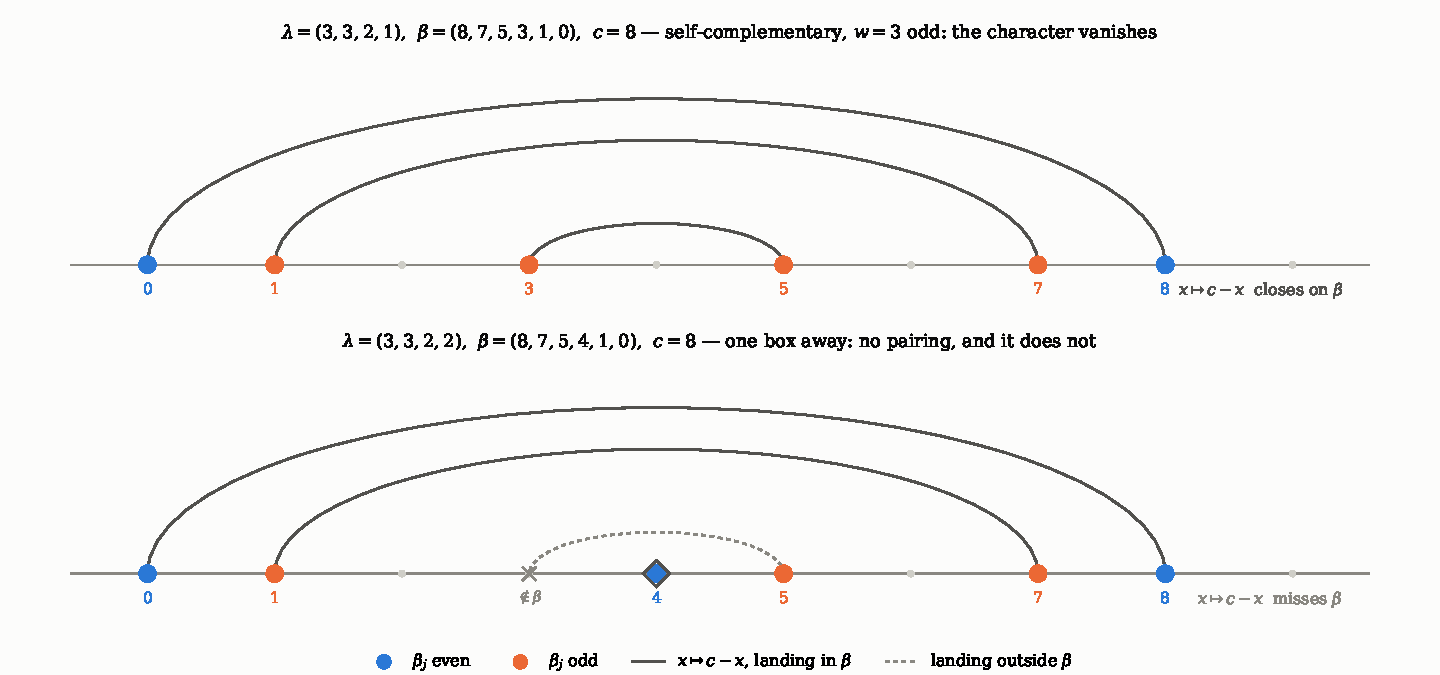
\includegraphics[width=\textwidth]{fig_involution.pdf}
\caption{Why self-complementarity kills the character. Expanding along the two frozen rows leaves
terms indexed by pairs $(e,o)$ with $e\in E$, $o\in O$, and the reflection $x\mapsto c-x$ acts on
them. Above, a self-complementary shape of odd width: every arc lands in $\beta$ and joins entries of
equal parity, because $c$ is even. Below, the same shape with one box moved: the arc $5\mapsto3$
leaves $\beta$, so there is no pairing and nothing cancels. The diamond marks the fixed point of the
reflection, which cannot occur inside an opposite-parity pair --- which is why the involution is
free.}
\label{fig:involution}
\end{figure}

\begin{proof}[Proof of Theorem \ref{thm:r1}]
Put $c_\ast=z+\bar z$ and let $S_n$ be defined by $S_0=0$, $S_1=1$,
$S_{n+1}=c_\ast S_n-S_{n-1}$, so $\deg_{c_\ast}S_n=n-1$ and $S_{-n}=-S_n$; the value $S_{-1}=-1$ is
used whenever $\beta_N=0$. Since $\Phi_A=(x^2-1)(x^2-c_\ast x+1)$, a polynomial $P$ supported on
$\beta$ is divisible by $\Phi_A$ exactly when $P(1)=P(-1)=0$ and $P\equiv0$ modulo $x^2-c_\ast x+1$.
Splitting $P(\pm1)$ by parity and reducing $x^n\equiv S_nx-S_{n-1}$, admissibility becomes the
singularity of the $4\times4$ matrix with rows $[\beta_j\ \mathrm{even}]$,
$[\beta_j\ \mathrm{odd}]$, $S_{\beta_j}$, $S_{\beta_j-1}$. Expanding along the two parity rows and
using d'Ocagne's identity \cite{Doc} for this recurrence,
\begin{equation}\label{eq:docagne}
S_bS_{b'-1}-S_{b'}S_{b-1}=-S_{b-b'},
\end{equation}
each $2\times2$ block collapses to a \emph{single} $S$, indexed by the difference of the two
surviving $\beta$'s. Distinct $S_n$ have distinct degrees in $c_\ast$ and are therefore linearly
independent, so the signed sum vanishes only by exact pairing of equal indices with opposite signs.
The case analysis is finite: $|E|\in\{0,4\}$ is branch (a); $|E|\in\{1,3\}$ leaves three terms whose
indices are the three pairwise differences of a $3$-set and hence always distinct, so no pairing
exists and the value is nonzero; and for $|E|=2$ there are four terms and three perfect matchings,
and one checks the six parity patterns directly. For $E=\{\beta_1,\beta_4\}$ and for
$E=\{\beta_2,\beta_3\}$ exactly one of the three matchings is available and it imposes the single
condition $\beta_1+\beta_4=\beta_2+\beta_3$, which is branch (b); for the four remaining patterns
every one of the three matchings forces two distinct entries of $\beta$ to coincide, so none is
available and the value is nonzero.
\end{proof}

Identity \eqref{eq:docagne} is classical. The collapse it produces is an accident of rank one: two
letters admit a single gap, so $s_{(m,n)}(z,\bar z)=S_{m-n+1}$ depends on that gap alone. There is no
rank-$r$ analogue. One would be a closed form for $s_\mu$ at a reciprocal alphabet for \emph{every}
$\mu$; \cite{CK09} supply that for rectangular shapes and \cite{AB19} for self-complementary ones,
and nobody in general.

For general $r$ we use associates, in Littlewood's sense \cite{Lit50}. On the $\det=-1$ coset $[\nu^{*}]=[\nu]\otimes\det$ gives
$\Psi_r=\sum_\nu\big(m_\nu-m_{\nu^{*}}\big)\chi_{[\nu]}$, so $\Psi_r=0$ if and only if
$m_\nu(\lambda)=m_{\nu^{*}}(\lambda)$ for every $\nu$; equivalently, $V_\lambda|_{O(N)}$ is
$\det$-invariant. A witness is therefore a single $\nu$ with $m_\nu\ne m_{\nu^{*}}$, and it can be
constructed.

Karmakar's \cite[Theorem 4.1]{Kar24} determines the value at the endpoint $z_i=1$, which is an element
of order two: case (A) is branch (a), case (B) is a nonzero dimension, and case (C) leaves an
alternating sum of products of dimensions with no vanishing criterion attached. Branch (b) lives in
that case (C), so the theorem below is not a consequence of it. Nor does case (B) help more as $r$
grows: at $k=1$ it asks that $N-1$ of the $N$ beta numbers share a parity, and the smallest shape
doing so is the staircase $(2r-1,2r-2,\dots,1)$, of size $r(2r-1)$, so on a fixed range of
$|\lambda|$ his nonvanishing case is visible only for small $r$ --- his result is sharpest exactly
where ours is easiest. What connects the endpoint to the
curve at all is rigidity, and rigidity is a statement about our object rather than about the order-two
element: over the ranges of \S\ref{sec:verif} it holds on $\ell(\lambda)\le N/2$ without exception
and fails outside, which is Remark \ref{rem:rankone}.

\begin{proof}[Proof of Theorem \ref{thm:stable}]
Branch (a) cannot occur: with $\ell(\lambda)\le N/2$ at least two trailing parts vanish, so $\beta$
contains two consecutive integers. In Littlewood's range
$m_\nu(\lambda)=\sum_{\beta'\ \mathrm{even}}c^{\lambda}_{\nu\beta'}$, and the term $\beta'=\emptyset$
gives $m_\mu\ge1$ for every $\mu\subseteq\lambda$. Take $\mu$ as follows. If
$\ell(\lambda)<N/2$, take $\mu=\lambda$: then $\ell(\lambda^{*})=N-\ell(\lambda)>\ell(\lambda)$, so
$\lambda^{*}\not\subseteq\lambda$ and $m_{\lambda^{*}}=0\ne m_\lambda$. If $\ell(\lambda)=N/2$ and
$\lambda_{N/2}$ is even, take $\mu=(\lambda_1,\dots,\lambda_{N/2-1})$; then
$\beta'=(\lambda_{N/2})$ is even, $\lambda/\mu$ is a horizontal strip and $m_\mu\ge1$ while
$\ell(\mu)<N/2$, so the previous computation applies to $\mu$. If $\ell(\lambda)=N/2$ and $\lambda$
is not a rectangle, let $j\le N/2-1$ be largest with $\lambda_j>\lambda_{j+1}$ and remove both the
last row and one box from row $j$; then $\beta'=(\lambda_{N/2}+1)$ is even and
$\lambda_j\ge\lambda_{N/2}+1$ keeps $\lambda/\mu$ a horizontal strip. In the remaining case
$\lambda=(k^{\,N/2})$ neither construction is available, and $k$ odd is branch (b) while $k$ even
falls to the second construction.
\end{proof}

\subsection{Outside Littlewood's range}\label{sec:unstable}

For $\ell(\lambda)>N/2$ the restriction rule acquires non-standard labels, and the modification rules
that reduce them are King's \cite{King71}; Koike and Terada \cite{KT87} record that the
type-$D$ specialization sends a universal character to $0$ or to $\pm$ one other, and Fauser, Jarvis,
King and Wybourne observe that beyond the two classical cases \emph{``the general theory, having
infinitely many cases, needs a not yet available formalism''} \cite[\S4]{FJKW05}. Extensions of Littlewood's rule to all parameters do exist for the two classical
cases --- Newell's modification rules \cite{New51}, Sundaram \cite{Sun90} in the symplectic case,
Gavarini's Brauer-algebra proof \cite{Gav99}, and Enright and Willenbring \cite{EW04}, whose Theorem 4
gives the multiplicity as an alternating sum over the Weyl group which in favourable cases collapses
to a difference of two Littlewood coefficients \cite[\S7.11]{EW04}. The route taken here is the dual
one: keep the coefficients universal, which they are in every range, and move the whole
range-dependence into the values, where one lemma disposes of it. On this alphabet no formalism for
the labels is needed at all, and the reason is that the values are not type-$D$ values.

Adding a letter $c$ to an alphabet acts on the ring of symmetric functions by $p_k\mapsto p_k+c^k$;
write $\iota_c$ for that homomorphism. From the generating function of the complete homogeneous
symmetric functions, $h_m(W,c)-c\,h_{m-1}(W,c)=h_m(W)$ for every $m$.

\begin{lemma}[the alphabet is symplectic]\label{lem:AtoSp}
$\iota_{-1}\iota_{1}\,o_\nu=sp_\nu$ for every partition $\nu$, as an identity between Koike--Terada
\emph{universal} characters in $\Lambda$. In particular, for the alphabet
\eqref{eq:psir},
\begin{equation}\label{eq:AtoSp}
o_\nu(A)\;=\;sp_\nu(z_1,\dots,z_r)
\end{equation}
with no hypothesis on $\ell(\nu)$ and with no sign. For $\ell(\nu)>r$ the right-hand side is
that universal character specialized at $r$ variables, not an irreducible $Sp(2r)$ character; it is
the modification rules below that fold it onto one.
\end{lemma}

\begin{proof}
Both steps are Ayyer and Kumari's, and both are the same manipulation: the recurrence turns the
column operations $C_j\to C_j-c\,C_{j-1}$, applied for $j=n,\dots,2$ in that order, into a change of
character type, and operations of that shape leave a determinant unchanged. At $c=1$ they carry the
defining determinant of $o_\nu$ evaluated at $(W,1)$ to that of the odd orthogonal universal
character $so_\nu$ over $W$, which is Koike and Terada's dictionary in the form
$so_\nu(X)=o_\nu(X,\bar X,1,0,0,\dots)$ \cite[(2.13)]{AK25}. At $c=-1$, where the recurrence is
\cite[Proposition 2.1]{AK25} and the operations read $C_j\to C_j+C_{j-1}$, they carry $so_\nu$ to
$sp_\nu$, which is \cite[Lemma 3.2]{AK25}. Composing gives the first statement, and evaluating it on
the reciprocal alphabet $(z_1,\dots,z_r)$ gives \eqref{eq:AtoSp}.
\end{proof}

\noindent Since $\nu'_1=\ell(\nu)$, the trichotomy on $\nu'_1$ against $N/2=r+1$ is a trichotomy on
the length of $\nu$ against the rank of $Sp(2r)$, and the three facts we need are then the classical
symplectic modification rules --- one of the two cases \cite{FJKW05} exempts --- read through
\eqref{eq:AtoSp}: $o_\nu(A)=0$ when $\ell(\nu)=r+1$, the vanishing of a symplectic character one row
past its rank; $o_\nu(A)=\pm o_{\nu^{*}}(A)$ when $\ell(\nu)>r+1$, King's rule folding the label back
onto a dominant one; and the same for non-standard $\nu$, which by Lemma \ref{lem:nonstd} are exactly
the tall ones. The expansion $s_\lambda=\sum_\nu c_\nu o_\nu$, with
$c_\nu=\sum_{\beta'\ \mathrm{even}}c^{\lambda}_{\nu\beta'}$, is an identity of symmetric functions and
holds in every range; specializing it at \eqref{eq:psir} therefore lands every term on
$\{o_\mu(A):\ell(\mu)\le r\}$, which by \eqref{eq:AtoSp} is the set of irreducible characters of
$Sp(2r)$ and so is linearly independent. Figure \ref{fig:reduction} sorts the labels into the four
classes this paragraph describes and computes $o_\nu(A)$ on each, so that the reduction can be seen
to land where it is claimed to. Hence

\begin{figure}[!ht]
\centering
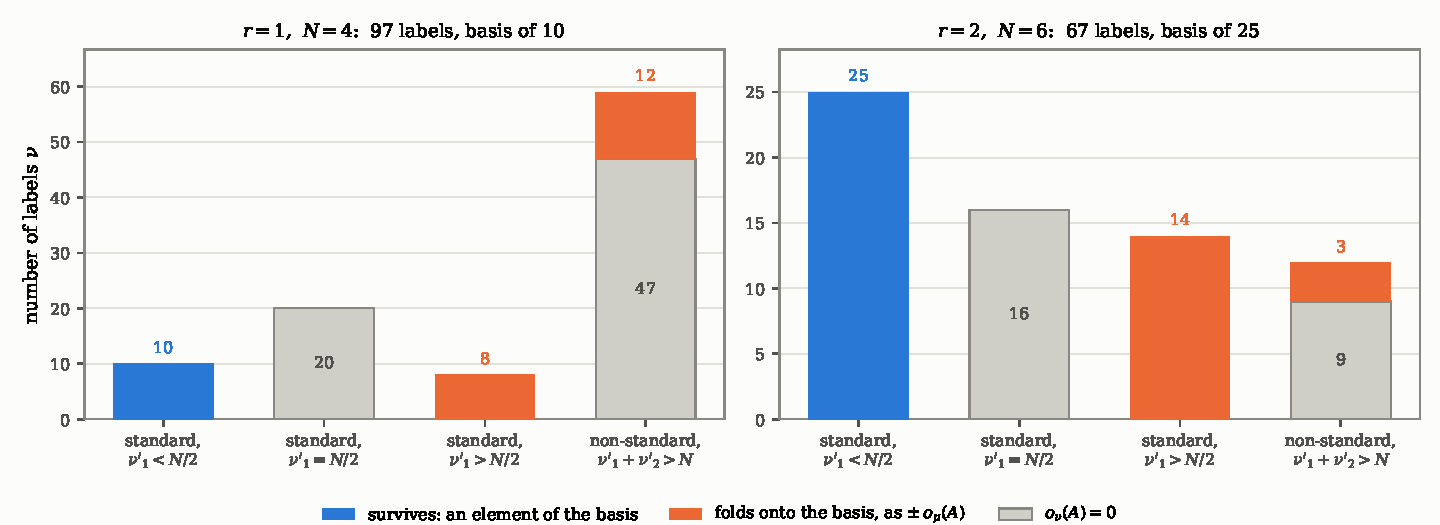
\includegraphics[width=\textwidth]{fig_reduction.pdf}
\caption{The reduction of Lemma \ref{lem:AtoSp}, drawn. Each label $\nu$
occurring in $s_\lambda=\sum_\nu c_\nu o_\nu$ is placed in one of four classes and its value
$o_\nu(A)$ computed. Self-associate labels vanish, every one of them; labels standard with
$\nu'_1>N/2$ fold onto the basis as $\pm o_{\mu}(A)$; non-standard labels either vanish or fold onto
a single basis element with coefficient $\pm1$. By \eqref{eq:AtoSp} these three are the symplectic
modification rules in disguise, the classes being cut by $\ell(\nu)$ against the rank $r$; the figure
was computed before that was noticed, and is left as drawn. Everything lands on the independent
basis $\{o_\mu(A):\ell(\mu)\le r\}$, which is what turns the vanishing into the finite condition
\eqref{eq:Cmu}. The bar heights are label counts over the range each panel was computed on, which is
smaller than the range of the corresponding row of \S\ref{sec:verif}; the classification, not the
count, is what the picture is about.}
\label{fig:reduction}
\end{figure}
\begin{equation}\label{eq:Cmu}
\Psi_r(\lambda)=\sum_{\ell(\mu)\le r}C_\mu(\lambda)\,o_\mu(A),
\qquad
\Psi_r(\lambda)=0\iff C_\mu(\lambda)=0\ \text{for all }\mu,
\end{equation}
where $C_\mu=c_\mu\pm c_{\mu^{*}}+\sum\pm c_\nu$ over the non-standard $\nu$ reducing to $\mu$. The
reduction is carried out in two steps rather than one: most non-standard labels pair with an associate
inside the range, while $21$ of them --- $18$ at $r=1$ and $3$ at $r=2$ --- have no associate in range
and are reduced separately, each landing in the span of the standard values with integer coefficients.

We had computed the three facts before locating them, and record the computation because it is what
the figure below draws: \texttt{sec8\_derivation.sage} checks \eqref{eq:AtoSp} directly for all
$|\nu|\le8$, confirms that the labels of length $r+1$ vanish and that longer ones fold onto the basis
with a sign, and verifies the independence as a rank computation, at $r=1,2,3$. A control that had to
fire: $\iota_1 o_\nu$ and $\iota_{-1}o_\nu$ each agree with $sp_\nu$ only for $\nu=\varnothing$, so
both letters are needed and \eqref{eq:AtoSp} is a statement about the reciprocal pair, not about
either letter alone. \texttt{sec8\_formulas.sage} checks the proof rather than the statement --- the
recurrence at four values of $c$, the two defining determinants against an independent
implementation, and the column operations entry by entry. That last check earned its keep: an earlier
draft of the proof wrote $C_j\to C_j+C_{j-1}$ at $c=1$, the sign \cite[Lemma 3.2]{AK25} uses for its
own step at $c=-1$.

The non-standard labels, which are the whole obstruction here, cannot be small:

\begin{lemma}[non-standard labels are large]\label{lem:nonstd}
Every non-standard $\nu$ occurring in the expansion satisfies $|\nu|\ge N+1=2r+3$. Consequently, if
$|\lambda|\le2r+2$ then no non-standard label is contained in $\lambda$, the last sum in $C_\mu$ is
empty, and $C_\mu(\lambda)=c_\mu(\lambda)\pm c_{\mu^{*}}(\lambda)$ --- with no hypothesis on
$\ell(\lambda)$, hence also outside Littlewood's range.
\end{lemma}

\begin{proof}
Since $c^{\lambda}_{\nu\beta'}=0$ unless $\nu\subseteq\lambda$, only labels with
$\ell(\nu)\le\ell(\lambda)\le N$ occur. Non-standard means $\nu'_1+\nu'_2>N$. Were $\nu$ a single
column we would have $\nu'_2=0$ and hence $\nu'_1=\ell(\nu)>N$, which is excluded; so $\nu'_2\ge1$ and
$|\nu|\ge\nu'_1+\nu'_2>N=2r+2$. A non-standard $\nu$ can therefore contribute only when
$|\lambda|\ge|\nu|\ge2r+3$.
\end{proof}

\noindent Since $\ell(\lambda)>N/2$ forces $|\lambda|\ge r+2$, Lemma \ref{lem:nonstd} settles the
band $r+2\le|\lambda|\le2r+2$ of the unstable range outright: there Littlewood's rule applies
verbatim and the converse follows by the argument of Theorem \ref{thm:stable}. What is left open is
$|\lambda|>2r+2$.


Two exact facts bound the competitors. First $\ell(\mu^{*})=N-\ell(\mu)$, so $\ell(\mu)\le
N-1-\ell(\lambda)$ forces $\mu^{*}\not\subseteq\lambda$ and $c_{\mu^{*}}=0$. Second, a non-standard
$\nu$ has $\nu'_1+\nu'_2>N$ with $\nu'_2\le\nu'_1$, hence $2\ell(\nu)>N$ and $\ell(\nu)\ge r+2$; in
particular no non-standard label fits inside $\lambda$ in Littlewood's range. Call $\mu$
\emph{isolating} for $\lambda$ if exactly one of the labels feeding $C_\mu$ is contained in
$\lambda$; then $C_\mu=\pm c_\nu\ne0$ and $\Psi_r(\lambda)\ne0$. What remains open is one existence
statement.

\begin{proposition}[the isolating witness does not always exist]\label{conj:iso}
At $r=2$ the shape $\lambda=(5,5,2,1)$ has $\Psi_2(\lambda)\ne0$ and is of neither type {\rm(a)} nor
type {\rm(b)}, and no $\mu$ is isolating for it: every $\mu$ whose $C_\mu$ has a nonzero contributor
inside $\lambda$ has exactly two, namely $\mu$ and its associate $\mu^{*}$.
\end{proposition}

We had proposed the isolating witness as the route to Conjecture \ref{conj:crit}, and it does not
reach. The reason is legible in the isolation lemma: it needs $\ell(\mu)\le N-1-\ell(\lambda)$, which
at $\ell(\lambda)=4$ and $N=6$ leaves only one-row $\mu$, and a shape as wide as $(5,5,2,1)$ contains
every associate. Over $r=2$ and $|\lambda|\le14$ there are eleven such shapes, and none at all below
$|\lambda|=13$, which is why the certificate looks sound on small ranges. Conjecture \ref{conj:crit}
itself is untouched --- it asserts that the $C_\mu$ vanish, not that a certificate exists, and it
holds over every shape in the ranges of \S\ref{sec:verif} --- but it is left without a route.

The mechanism does reach a great deal: at $r=2$ and $|\lambda|\le14$, $227$ of the $238$ non-vanishing
unstable shapes carry a proved isolating witness. It also reaches further than fact (ii) allows on
its own --- the true minimum of $\ell(\nu)$ over non-standard $\nu$ with $o_\nu(A)\ne0$ is $5$ there,
against the $r+2=4$ the bound gives. What defeats it is width rather than height: the basis in
\eqref{eq:Cmu} grows with $r$ and the competing labels are constrained to be tall, so we had read
isolation as getting easier with $r$, and along the height axis it does; the residue lives where
$\lambda$ is wide enough to swallow the associates. That reading predicts where the residue is
\emph{not}: at $r=3$ the isolation lemma allows $\ell(\mu)\le7-\ell(\lambda)$, so a shape must be
wider than at $r=2$ before it can swallow every associate, and the same sizes should come out clean.
They do --- over $r=3$ and $|\lambda|\le13$ all $149$ non-vanishing unstable shapes carry a proved
witness and the residue is empty --- which is a control on the explanation rather than a step toward
the conjecture. At $r=1$ the question does not arise, since that case is settled independently by
Theorem \ref{thm:r1}.

The tool one reaches for first does not fit. Saturation, in the honeycomb form of Knutson and Tao
\cite{KT99}, decides when a single Littlewood--Richardson coefficient is positive, and every
competitor feeding $C_\mu$ is positive as soon as its label sits inside $\lambda$. What an isolating
$\mu$ asks for is not positivity but \emph{isolation}: that exactly one of them does. The positivity
is what makes the question hard rather than what answers it, and we know of no tool aimed at the
second question.

\begin{figure}[tb]
\centering
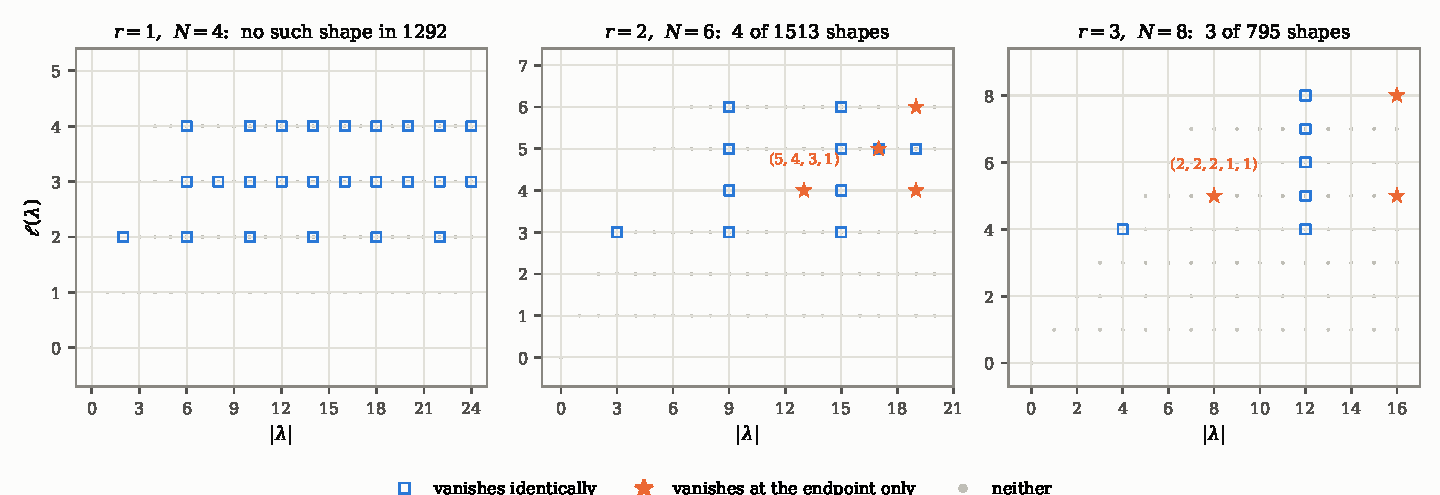
\includegraphics[width=\textwidth]{fig_phase.pdf}
\caption{Where one reciprocal pair stops being typical. Each partition with at most $N$ parts is a
point at $(|\lambda|,\ell(\lambda))$; the class drawn as a star is the one that vanishes at the
endpoint $z_i=1$ without vanishing identically, and it is the whole content of the picture; each
panel names its smallest member and Remark \ref{rem:rankone} lists the rest. The panels cover
$|\lambda|\le24$, $20$ and $16$ respectively. At $r=1$ the class is
empty over all $1292$ shapes in range, because the object there is $\pm$ a genuine character and its
value at the identity is a dimension. From $r=2$ on the object is properly virtual and the class is
not empty. See Remark \ref{rem:rankone}.}
\label{fig:phase}
\end{figure}

\begin{remark}[the rank-one accident, and where the two ranges part]\label{rem:rankone}
At $r=1$ the object is $\pm$ a genuine character, so its value at the identity is a dimension and
$\Psi_1(\lambda)\equiv0$ if and only if $\Psi_1(\lambda)|_{z=1}=0$. At $r\ge2$ the object is properly
virtual and that equivalence fails: $\lambda=(5,4,3,1)$ at $r=2$ has $\Psi_2(\lambda)\ne0$ and
$\Psi_2(\lambda)|_{z_1=z_2=1}=0$. Over the ranges of Figure \ref{fig:phase} the class of such shapes
is empty at $r=1$ across $1292$ partitions; at $r=2$ it consists of the four shapes $(5,4,3,1)$,
$(5,5,4,2,1)$, $(10,5,3,1)$ and $(6,5,4,2,1,1)$, and at $r=3$ of the three shapes $(2,2,2,1,1)$,
$(5,5,4,1,1)$ and $(3,3,3,2,2,1,1,1)$; it is thin, but it is not empty, and one counterexample is all
the equivalence can survive. The surviving implication, exact vanishing $\Rightarrow$ vanishing
at the endpoint, is what makes the endpoint a valid sieve and no more. This is why results computed
at elements of order two \cite{Kar24}, or at variables set to $1$ \cite{Eis07}, bear on the endpoint
and not on the curve, and why Theorem \ref{thm:zeros} is not a corollary of them for $r\ge2$.
\end{remark}

It is worth putting a number on what the endpoint sieve loses, since the qualitative statement is
easy to misread as a small correction. Over the ranges of Figure \ref{fig:phase} the test
$\Psi_r(\lambda)|_{z_i=1}=0$ flags $143$ shapes at $r=1$, $22$ at $r=2$ and $9$ at $r=3$; of those,
$0$, $4$ and $3$ respectively do not vanish identically. So the sieve is exact at one pair, and the
fraction of its verdicts that are spurious grows with the number of pairs --- $0\%$, $18\%$, $33\%$
over these ranges. An endpoint computation is a filter that never misses a genuine zero, and past one
pair it is nothing more than that. The rank-one case at $t=2$, where the sieve happens to be exact
because the object is a genuine character, was treated separately in \cite{Mar26}; the alphabet
\eqref{eq:object} arose there, in a Wilson-line computation on an orbifold, which is why $-1$ appears
as a letter rather than as a choice.

The reason the two ranges of $\ell(\lambda)$ behave so differently is worth separating from the
mechanism that proves it. Littlewood's rule is a statement about which labels $\nu$ can occur, and
$\ell(\lambda)\le N/2$ is exactly the condition under which the non-standard ones cannot fit inside
$\lambda$ at all. Lemma \ref{lem:nonstd} says that the obstruction is governed by $|\lambda|$ as well
as by $\ell(\lambda)$, so the honest picture is not two ranges but a region: the converse is proved
wherever either $\ell(\lambda)\le N/2$ or $|\lambda|\le2r+2$, and outside their union it is open ---
the isolating witness covers most of that region but provably not all of it, by Proposition
\ref{conj:iso}.

%======================================================================
\section{Verification}\label{sec:verif}

Every statement above was checked numerically, by two implementations along different code paths: one
in exact Laurent arithmetic, and one a from-scratch bialternant evaluation written from the
statements alone. The ranges and counts are collected here once.

\begin{center}\footnotesize\setlength{\tabcolsep}{4.2pt}
\begin{tabular}{llrl}
\toprule
statement & range & result & status\\
\midrule
Theorem \ref{thm:main}, sign included & $t\le7$, $|\lambda|\le14,\dots,10$ &
$959$ exact, $476$ zeros, $0$ fail & \stproved\\
Lemma \ref{lem:L1} & $t\le6$ & $454$ nonzero minors & \stproved\\
Lemma \ref{lem:L4} & $t\le7$ & $724/724$ & \stproved\\
Proposition \ref{prop:quotient} & $t\le7$, $|\lambda|\le19$ & $2970/2970$ & \stproved\\
Proposition \ref{rem:lattice} (the concentric locus) & $t\le9$, $|\lambda|\le16$ & $1331/1331$;
$0$ at odd $t$, $43$ at even & \stproved\\
Proposition \ref{rem:sign} (short form of the sign) & $t\le8$, $|\lambda|\le14$ & $1496/1496$;
proof steps $0$ fail & \stproved\\
Proposition \ref{prop:fibrelattice} (the lattice) & $t\le5$, $|\lambda|\le14,12,10,10$ &
$84$, $35$, $20$, $14$ fibres, both ways & \stproved\\
Corollary \ref{cor:fibregf} (the generating function) & same range &
$153/153$; wrong denominator $101$ & \stproved\\
Remark \ref{rem:signsees} (the sign sees the $m_i$) & $t\le4$ &
$107/107$, $43/62$, $26/36$ & \stverif\\
Lemma \ref{lem:single} & $t\le7$, $|\lambda|\le16$ & $2113/2113$ & \stproved\\
Theorem \ref{thm:extra} & $t\le12$, $\lambda_1\le33$ & $119+21$, no others & \stproved\\
Proposition \ref{prop:rect} & $t=2$, $r\le4$, $c\le60$ & $240/240$ & \stproved\\
Corollary \ref{cor:enum} against direct enumeration & $t\le5$ & $14/14$; boxes $16/16$ &
\stproved\\
Proposition \ref{rem:involution} (the runs alternate) & $t=2$, $|\lambda|\le14$, $\le4$ rows &
$4823$ minors; $217$ pairs, $0$ fail & \stproved\\
(D3), (D4) of \S\ref{sec:sharp} & $t\le6$, $|\lambda|\le10$ &
$600$ / $383$ / $200$ of $600$ & \stverif\\
\midrule
\rowcolor{hband} Theorem \ref{thm:zeros}, both directions & $r\le3$, $|\lambda|\le28,26,22$ &
$9961$ shapes, $318$ zeros, $0$ fail & \stverif\\
\rowcolor{hband} \quad branch (a), Thm.~\ref{thm:zeros} & $r\le3$, $|\lambda|\le15$ &
$16/16$ & \stproved\\
\rowcolor{hband} \quad branch (b), Thm.~\ref{thm:zeros} & $r\le3$ & $24/24$ & \stproved\\
\rowcolor{hband} \quad even-width control for (b) & $r\le3$ & $56/56$ nonzero & \stproved\\
\rowcolor{hband} \quad converse at $r=1$, Thm.~\ref{thm:r1} & $\beta_1\le25$ &
$14950$ beta sets, $0$ fail & \stproved\\
\rowcolor{hband} \quad converse, $\ell(\lambda)\le N/2$, Thm.~\ref{thm:stable} & $r\le3$ &
$372/372$ witnesses & \stproved\\
\rowcolor{hband} \quad the isolating witness, Prop.~\ref{conj:iso} & $r=2$, $|\lambda|\le14$ &
$227$ witnesses, $11$ residue & \stproved\\
\rowcolor{hband} \quad the same at $r=3$ & $r=3$, $|\lambda|\le13$ &
$149$ witnesses, $0$ residue & \stproved\\
\midrule
Identity \eqref{eq:compl} & $r\le2$ & $474/474$ & \stproved\\
Identity \eqref{eq:docagne}, and $\deg_{c_\ast}S_n=n-1$ & $b\le31$ & $496/496$; $39/39$ &
\stproved\\
Lemma \ref{lem:AtoSp}, the \S\ref{sec:unstable} reduction & $r\le3$, $|\nu|\le8$ &
identity $0$ fail; folds $0$ fail & \stproved\\
\quad the reduction carried out & $r\le2$ & $236$ labels, $0$ unresolved & \stproved\\
\eqref{eq:Cmu} against the exact object & $r\le2$, both ranges & $184$ shapes, $0$ fail &
\stverif\\
\bottomrule
\end{tabular}
\end{center}

\noindent The shaded block is Theorem \ref{thm:zeros} read from the top down: the two sufficient
branches are proved for every $r$, the converse is proved for one pair and, for every $r$, inside
Littlewood's range, and one line remains --- the converse for $r\ge2$ outside that range and beyond
the band $|\lambda|\le2r+2$ that Lemma \ref{lem:nonstd} settles, which is Conjecture
\ref{conj:crit}. That single \stverif\ line is why the first row of the block is not
labelled \stproved. The row below it records what the certificate we proposed for that line does and
does not do, and it is labelled \stproved\ because Proposition \ref{conj:iso} is a counterexample and
counterexamples are proofs. The rows below the block are the identities and the reduction the section rests
on. In the column, \stproved\ means a proof is given here or cited, and \stverif\ means the
statement is checked exhaustively over the stated range and not proved.

\noindent The (D3), (D4) row is the one that matters most in the first group: the identity holds in
all $600$ cases for \eqref{eq:object} and fails in $217$ and $400$ of them for the two deformed
alphabets, so the test is capable of failing. In the second group the even-width control plays the
same role for Theorem \ref{thm:zeros}: $56$ self-complementary shapes of even width, none of which
vanishes, so the parity hypothesis is doing work rather than decorating. A separate audit rebuilds
all of the second group from the definitions in a single pass, independently of the scripts that
produced them: $3414$ checks, $0$ failures. A second one takes the \emph{displayed formulas} rather
than the counts --- Theorem \ref{thm:LR}, the interval reading \eqref{eq:intervals}, Lemmas
\ref{lem:L2} and \ref{lem:L5}, the splitting \eqref{eq:threestep}, the complementation
\eqref{eq:compl}, d'Ocagne \eqref{eq:docagne} and the scalar caveat \eqref{eq:scalar} --- and
evaluates both sides at numeric points from the definitions, using neither the closed forms of this
paper nor the scripts behind the table: $3297$ evaluations over nine displayed formulas, $0$ failures. The scripts are ancillary to this paper, and so is the
saved output of each one, so every count in the table above can be located in an archived run rather
than taken on trust.

%======================================================================
\section{Open problems}\label{sec:open}

\begin{problem}[the other classical types]\label{prob:types}
Everything above is type $A$. What do $sp_\lambda(\zt,z,\zb)$, $so_\lambda(\zt,z,\zb)$ and
$o_\lambda(\zt,z,\zb)$ do? The root-of-unity factorizations were carried from type $A$ to $B$, $C$,
$D$ by a uniform argument in \cite{AK22} and to the universal characters in \cite{Alb23}; the frozen
rows of the bialternant are the same in every type, so Lemma \ref{lem:L1} and the excess-two count
should survive verbatim, while the collapse, Lemmas \ref{lem:L4} and \ref{lem:L5}, would need
re-deriving once per type. The alphabet \eqref{eq:object} is already a torus element of $O(t+2)$, so
the other types are not the same function at a new point but new objects, and choosing the right ones
is a matter of taste inside a programme we did not build. We have measured, and report it as a
measurement only. Expanding the Koike--Terada universal characters in the Schur basis and evaluating
term by term with Theorem \ref{thm:main}, over $|\lambda|\le12$ for $t\le3$ and $|\lambda|\le10$ for $t=4,5$, the fraction of
$\ell(\lambda)\ge2$ shapes on which the value vanishes is markedly larger for $o_\lambda$ on the
non-identity component than on the identity one --- $83.8\%$ at $t=2$ against $41.8\%$ at $t=3$, and
$58.8\%$ at $t=4$ against $42.1\%$ at $t=5$ --- with $sp_\lambda$ in between and the Schur case
lowest. The effect is real and it tracks the component, which is what one would expect of an
associate cancellation; but it is quantitative and we found no law covering the whole table. A first
attempt at one, that
$o_\lambda$ vanishes for all $\ell(\lambda)\ge2$ when $t$ is even, is false: it was read off a
sample and the systematic sweep refutes it.

The $t=2$ column of that comparison is the one case which does have a law, and it is Lemma
\ref{lem:AtoSp}: there the alphabet is \eqref{eq:psir} at $r=1$, so $o_\nu$ equals $sp_\nu(z)$, a
\emph{rank-one} symplectic character. That vanishes identically for $\ell(\nu)=2$ --- all $36$ such
shapes in range, with no exception --- and folds for $\ell(\nu)>2$, which is why the $t=2$ figure is
the outlier. What remains without a law is odd $t$, where the alphabet is not of the form
\eqref{eq:psir} and the lemma does not apply.

The $sp_\lambda$ column at $t=2$, on the other hand, has an answer, and it explains the asymmetry of
the table rather than adding a row to it. Adjoining the same two letters to a universal
\emph{symplectic} character does not collapse it. Over $|\nu|\le8$,
\begin{equation}\label{eq:spbranch}
sp_\nu(W,1,-1)\;=\;\sum_{\gamma\subseteq\nu}c_{\nu/\gamma}\;sp_\gamma(W),
\end{equation}
where the coefficient depends on $\nu$ and $\gamma$ only through the skew shape $\nu/\gamma$ ---
$247$ coefficients over $74$ distinct skew shapes, with no clash --- and takes only the values $0$
and $\pm1$, vanishing whenever $|\nu/\gamma|$ is odd. That is the shape a branching rule for
universal symplectic functions produces, and such rules are available \cite{JJLW24}. Read against it,
Lemma \ref{lem:AtoSp} says that for $o_\nu$ the corresponding coefficients are concentrated at
$\gamma=\nu$: the two letters collapse the orthogonal character to a single symplectic one, and leave
the symplectic character spread over the whole interval below $\nu$. The asymmetry of the measurement
is that, and not an artefact of the ranges. What we have not done is identify $c_{\nu/\gamma}$, which
\eqref{eq:spbranch} makes a question about skew universal symplectic characters at $(1,-1)$ and
nothing more.

The third column resists the same route, and for a structural reason rather than an accidental one.
What answers the other two is that adjoining a letter is the ring map $p_k\mapsto p_k+c^k$, so
$\iota_{1}$ and $\iota_{-1}$ act on $\Lambda$ and compose. The identity that would bring $so$ into
the picture, $so_\nu(X)=o_\nu(X,\bar X,1,0,\dots)$ of \cite[(2.13)]{AK25}, relates the two on a
\emph{doubled} alphabet instead, and a doubling is not an adjunction: the $\iota$'s do not reach it.
So the $so$ column is not a gap of effort but of mechanism, and we leave it stated as such.
\end{problem}

\begin{problem}[a Verschiebung that sees a reciprocal pair]\label{prob:versch}
The operator $\varphi_t$ has nothing to say about a letter outside a $\zeta$-orbit, which is the
structural reason Theorem \ref{thm:main} is not a corollary of anything in that line, and the reason
our proof descends to the alternant. Is there an operator on universal characters, or a
factorization of $\varphi_t$ through a larger algebra, acting on alphabets of the form (union of
$\zeta$-orbits) $\cup$ (reciprocal pairs)? By \S\ref{sec:sharp} such an operator would decide (D1)
and (D2) at once. The discussion there suggests a quantitative form.

What makes the question well posed rather than vague is that each half already has a formalism, and
they are not the same one. The $\zeta$-orbits are the province of $\varphi_t$, in Albion's
formulation \cite{Alb23}. Alphabets closed under inversion are the province of the universal
symplectic and orthogonal functions, which have vertex operator realizations from which their
branching rules follow \cite{JJLW24}. Our alphabet is one of each, and Lemma \ref{lem:AtoSp} is the
one place where the two meet: there the $\zeta$-orbit is $\{1,-1\}$, small enough that adjoining it
is a pair of letter maps rather than an operator. We know of nothing that acts on both halves at
once, and the question is whether the two formalisms compose.
\end{problem}

\begin{proposition}[the rank is the wrong invariant]\label{conj:rank}
Let $A=\zt\cup B$ with $B$ closed under inversion and disjoint from $\zt$, and let $\rho(B)$ be the
rank of the subgroup of $\CC^{\times}$ generated by $B$. Then $\rho(B)=1$ does not imply that
$s_\lambda(A)$ is a product of characters. At $t=2$ and $B=\{z,z^{-1},z^{2},z^{-2}\}$, which has
$\rho(B)=1$, the value at $\lambda=(2)$ has a root off the unit circle, and so has no such
factorization; the same happens for $B=\{z,z^{-1},z^{3},z^{-3}\}$.
\end{proposition}

\begin{proof}
A product of characters $\chi_k(z)=(z^{k+1}-z^{-k-1})/(z-z^{-1})$ has all of its roots on the unit
circle. For $B=\{z,z^{-1},z^{2},z^{-2}\}$ and $\lambda=(2)$ the value is
$z^{-4}+z^{-3}+z^{-2}+z^{-1}+3+z+z^{2}+z^{3}+z^{4}$, whose roots miss the circle by $0.32$; over
$|\lambda|\le8$ this happens for $17$ of the $62$ nonvanishing shapes, and for
$B=\{z,z^{-1},z^{3},z^{-3}\}$ for $18$. On the same range $B=\{z,z^{-1}\}$ has every root on the
circle without exception, as Theorem \ref{thm:main} requires.
\end{proof}

What the rank does not see is how many free directions $B$ has. A single reciprocal pair is one
direction; $\{z,z^{-1},z^{2},z^{-2}\}$ generates a group of rank one and is two, and the two see each
other. So the invariant to conjecture on is not $\rho(B)$ but the number of independent letters,
and with that reading the statement becomes the one \S\ref{sec:sharp} already makes by other means:

\begin{conjecture}[one free direction]\label{conj:rank2}
$s_\lambda(\zt\cup B)$ is a product of characters for every $\lambda$ if and only if $B$ is a single
reciprocal pair.
\end{conjecture}

The evidence for it is Theorem \ref{thm:main} in one direction and (D1)--(D4) together with
Proposition \ref{conj:rank} in the other: enlarging $B$ destroys the product whether the enlargement
raises the rank or not. We have no proof and no proposed mechanism, and this is precisely the
statement a $\varphi_t$-style argument ought to produce.

One caveat, which the conjecture as stated does not cover. Inversion-closure of $B$ is sufficient in
the evidence above, but it is not necessary for a product. Write $w=-iy$. Then the second block of
the alphabet $\{1,-1,y,-y^{-1}\}$ is not closed under inversion, yet
\begin{equation}\label{eq:scalar}
s_\lambda\big(1,-1,y,-y^{-1}\big)\;=\;i^{\,|\lambda|}\,s_\lambda\big(-i,\,i,\,w,\,w^{-1}\big),
\end{equation}
and the alphabet on the right is. The honest hypothesis is therefore that $A$ be a scalar multiple of
an inversion-closed set. A coset $\zeta\zt$ is itself inversion-closed exactly when
$\zeta^{2}=\pm1$, which is where (D3) does and does not break.

\begin{problem}[the instrument for the second pair]\label{prob:instrument}
Section \ref{sec:zeros} reduces the vanishing at $r\ge2$ to a statement about the coefficients
$C_\mu$ of \eqref{eq:Cmu}, which are signed sums of Littlewood coefficients, and Conjecture
\ref{conj:crit} is what remains --- with no certificate for it, since the one we proposed fails by
Proposition \ref{conj:iso}. Lemma \ref{lem:AtoSp} settles the other half of the reduction --- what
the values $o_\nu(A)$ are --- and settles it symplectically: the two readings of the alphabet agree
because they are the same reading, the orbit Lie algebra of $D_{r+1}$ being $C_r$ rather than the
fixed subalgebra $B_r$. What it does not touch is the coefficients. Kumari and Stokke \cite{KS26}
have given Murnaghan--Nakayama rules for symplectic, orthogonal and orthosymplectic Schur functions;
by Lemma \ref{lem:AtoSp} the relevant one here is the symplectic \cite[Theorem 3.4]{KS26}, not the
even orthogonal \cite[Theorem 3.10]{KS26}. Does the recursion it provides compute $C_\mu$? Their rule
carries a third sum beyond the adding and removing of border strips, and it is the one they single out
as complicated; \cite[Corollary 3.5]{KS26} shows it drops out once $\mu_n+1\ge r$, so it is a
shallow-shape phenomenon. An earlier form of this problem asked whether that sum is what accounts for
the failure of Littlewood's rule outside its range; Lemma \ref{lem:AtoSp} answers that it is not,
since the failure is carried by the symplectic modification rules, which act on the labels and not
inside the recursion. The coefficients are what is left, and whether that recursion computes them is
what we have not attempted.
\end{problem}

\begin{problem}[the extra locus, in general]\label{prob:extralocus}
Does Theorem \ref{thm:extra} have an analogue for $sp$, $so$ and $o$? More generally, for which
specializations of the free variables does the criterion \eqref{eq:AK53} acquire extra solutions, and
can the extra locus always be read off the kernel of the specialization acting on the span of the
universal characters, as Remark \ref{rem:why} suggests? If each type acquires a family indexed by an
order-two element of the residue lattice, the principle is real.

The question needs the free part pinned down, and for a computed reason: the extra family is a
phenomenon of the \emph{minimal} alphabet. Adjoin a second reciprocal pair and it is gone --- over
$t=3,4,5,6$ and $|\lambda|\le14$ the locus is then exactly the $t$-cores, for type $s$ no less than
for $sp$ and $o$, while at one pair type $s$ has the two extras of Theorem \ref{thm:extra} at $t=4$
and one at $t=6$. (We test the second pair at $z_2=z_1^{2}$, a specialization, which can only create
coincidences and not remove them, so a count of zero there is a count of zero.) An analogue for
another type must therefore be sought at \emph{that type's} minimal free part, one letter of each
kind; comparing types across free parts of different sizes measures the free part instead, which is
what our first attempt did.

The kernel is the right thing to look at, but its \emph{presence} does not settle the locus; its
size does. Two free parts of the same size can both collapse the independence and behave quite
differently. On the reciprocal locus $s_\mu(z,\zb)=\chi_{\mu_1-\mu_2}(z)$ retains one grading, and
the extra locus is the single family of Theorem \ref{thm:extra}. Replace the pair by the
$\zeta_2$-orbit $(z,-z)$, where $s_\mu(z,-z)=z^{|\mu|}s_\mu(1,-1)$ retains only $|\mu|$ and a sign,
and over $\ell(\lambda)\le2$ the criterion acquires $28$ further solutions at $t=2$ and $186$ at
$t=8$, in no family we can name. The control is the free pair $(z,w)$, which has no kernel and
returns the $t$-cores and nothing else at every $t\le8$ --- that is \eqref{eq:AK53} itself, so the
control is their theorem rather than a measurement of ours. So the
reciprocal pair is the collapsing specialization of \emph{smallest} kernel, and that, rather than
the mere existence of a kernel, is what makes its extra locus one family.
\end{problem}

\begin{problem}[the fibres, refined by the sign]\label{prob:fibres}
Corollary \ref{cor:fibregf} describes the fibre of the interval triple, and only that. The invariant
is $I_t=(d_1,d_2,d_3,\varepsilon_\lambda)$, and the sign cuts each branch further. Its cut is not
bookkeeping, and it is not idle: by Remark \ref{rem:signsees} the sign sees the $t-2$ directions the
triple does not, from $t=3$ on --- constant in $(m_i)$ at fixed $v$ in all $107$ slots at $t=2$, but
in only $43$ of $62$ at $t=3$ and $26$ of $36$ at $t=4$. What is the restriction of
$\varepsilon_\lambda$ to a branch? The obstruction to reading it off \eqref{eq:fibrelattice} is
visible in \eqref{eq:sign}: $\inv(b_S)$ is a statistic of the whole beta-word, and the lattice
coordinates split that word into two distinguished classes and $t-2$ free letters, so a rule would
have to reassemble what the bijection separates.

Two smaller gaps go with it. The same description for the size-three profile should be the same
bookkeeping with one class of three in place of two of two; we have not written it. The degenerate
profile is a different question, since there the fibre is the whole vanishing locus of $\Phi_t$,
which Corollary \ref{cor:zero} and Proposition \ref{rem:lattice} describe by other means.
\end{problem}

\begin{problem}[a sieving phenomenon that keeps a parameter]\label{prob:sieving}
At $t=2$ Corollary \ref{cor:enum} is a signed count of $\mathrm{SSYT}(\lambda,4)$, and a signed count
of order two is what Stembridge's $q=-1$ phenomenon \cite{Ste94} computes: on a set carrying an
involution, the value at $-1$ counts the fixed points. That is the case $\#C=2$ of the cyclic sieving
phenomenon of Reiner, Stanton and White \cite{RSW04}, whose Theorem 4.3 evaluates the principal
specialization $s_\lambda(1,q,\dots,q^{k-1})$ at a primitive $d$-th root of unity in terms of the
$d$-core and the $d$-quotient of $\lambda$ --- the two invariants that carry Theorem \ref{thm:main}
as well --- and which Lee and Oh \cite{LO22} have since extended to skew shapes. Every evaluation in
that line is at a \emph{number}, as a sieving statement requires: the alphabet there is the geometric
progression $1,q,\dots,q^{k-1}$ specialized at a root of unity, not a plain orbit, and nothing is
left free. Ours is not of that kind --- the reciprocal pair keeps $z$, and \eqref{eq:main} is a
product formula in it. Is there a cyclic action on $\mathrm{SSYT}(\lambda,t+2)$, and a $q$-analogue of
$\Phi_t$, whose value at a $t$-th root of unity counts fixed points refined by $m_{t+1}-m_{t+2}$?
The case $\#C=2$ is where to look first, and there the involution such a statement would need already
exists: \S\ref{sec:enum} assembles it.

The existence half of the question is decidable without exhibiting the action. Alexandersson and
Amini \cite{AA19} give a necessary and sufficient criterion for a cyclic action realizing a given
sieving polynomial to exist: for every $d\mid t$, the value at $\omega^d$ must be
$\sum_{j\mid d}j\,c_j$ with every $c_j$ a nonnegative integer, and the $c_j$ --- the numbers of
orbits of each size --- are then computable by triangularity. Applied to the candidate that the
alphabet itself suggests, $F(q,z)=s_\lambda(1,q,\dots,q^{t-1},z,z^{-1})$, whose $z$-grading is
already the refinement asked for, the criterion is met by almost every graded piece in the ranges we
can reach; but so it is for a deliberately wrong refinement, grading by $m_{t+1}+m_{t+2}$ instead,
which passes at the same rate. At those sizes the criterion does not discriminate, and we report the
attempt as evidence in neither direction.
\end{problem}

One narrower gap is recorded where it arises rather than here, in the same form as the problems
above and with the same meaning --- something we would like to know and have not settled: the
involution of \S\ref{sec:enum} is assembled at $t=2$ and nowhere else, because Proposition
\ref{rem:involution} is a statement about one word and that word is the $t=2$ one. The distinction we
keep throughout is between a \emph{conjecture}, which is a statement we believe and have tested, and
a \emph{problem}, which is not a claim at all.

Taken together the problems say where we think the object stops being ours. The evaluation is
complete and the alphabet is minimal, so what is left is not more of the same: it is whether the two
formalisms that own the two halves of \eqref{eq:object} compose, whether a sieving statement can keep
a variable, and what the coefficients $C_\mu$ do once the certificate we proposed for them is gone.
Of the three, the last is the one the paper needs and the first is the one we would rather see
answered.

\subsection*{Acknowledgements}
This paper exists because Arvind Ayyer asked whether the rank-one case generalizes to arbitrary $t$
with the free variable symbolic. The question was better than the note that prompted it. We thank him
for it, and for the correspondence that followed. Remark \ref{rem:core} exists because Nishu Kumari
asked whether the condition $n_i(\lambda)=0$ could be phrased in terms of the $t$-core; she also
confirmed the reading of \cite[Theorem 5.3]{AK25} in \S\ref{sec:independence}, and it was a pointer
of hers that sent us to \cite[\S3]{AK25}, where Lemma \ref{lem:AtoSp} was waiting; we are grateful
for it. The involution of \S\ref{sec:enum} is assembled from three lemmas of her thesis
\cite{KumariThesis}, and is hers in that sense too.

\subsection*{Code, data and disclosure}
Every computation quoted in this paper is performed by a named script distributed as an ancillary
file, and every number quoted is reproduced by an archived run of one; \S\ref{sec:verif} tabulates
which script answers for which claim. The same scripts and the same archived output are also kept at
\url{https://github.com/karlesmarin/schur-orbit-and-reciprocal-pair}, which is a convenience: the
ancillary files carry everything the paper appeals to. Generative AI (Claude, Anthropic) was used
throughout as a
research assistant --- for literature search, for writing and checking the ancillary code, and on the
prose. The mathematics, and the responsibility for it, are the author's.

%======================================================================
\begin{thebibliography}{AAAA}

\bibitem[Alb23]{Alb23} S.~P.~Albion, \emph{Universal characters twisted by roots of unity},
Algebraic Combinatorics; arXiv:2212.07343.

\bibitem[Alb25]{Alb25} S.~P.~Albion, \emph{Character factorisations, $z$-asymmetric partitions and
plethysm}, arXiv:2501.18520.

\bibitem[AA19]{AA19} P.~Alexandersson and N.~Amini, \emph{The cone of cyclic sieving
phenomena}, Discrete Math. \textbf{342} (2019), no.~6, 1581--1601; arXiv:1804.01447.

\bibitem[AB19]{AB19} A.~Ayyer and R.~E.~Behrend, \emph{Factorization theorems for classical group
characters, with applications to alternating sign matrices and plane partitions}, J. Combin. Theory
Ser.~A \textbf{165} (2019), 78--105; arXiv:1804.04514.

\bibitem[AK22]{AK22} A.~Ayyer and N.~Kumari, \emph{Factorization of classical characters twisted by
roots of unity}, J. Algebra \textbf{609} (2022), 437--483; arXiv:2109.11310.

\bibitem[AK25]{AK25} A.~Ayyer and N.~Kumari, \emph{Further results for classical and universal
characters twisted by roots of unity}, J. Algebraic Combin. \textbf{63} (2025), no.~1;
arXiv:2501.00275.

\bibitem[CK09]{CK09} M.~Ciucu and C.~Krattenthaler, \emph{A factorization theorem for classical
group characters, with applications to plane partitions and rhombus tilings}, in: Advances in
Combinatorial Mathematics, Springer, Berlin, 2009.

\bibitem[GKS90]{GKS90} F.~Garvan, D.~Kim and D.~Stanton, \emph{Cranks and $t$-cores},
Invent. Math. \textbf{101} (1990), no.~1, 1--18.

\bibitem[HI24]{HI24} M.~Hidaka and M.~Itoh, \emph{The Schur polynomials in all primitive $n$th roots
of unity}, J. Combin. Theory Ser.~A; arXiv:2403.10817.

\bibitem[Jan73]{Jantzen} J.~C.~Jantzen, \emph{Darstellungen halbeinfacher algebraischer Gruppen},
Bonner Math. Schriften \textbf{67} (1973).

\bibitem[Kar22]{Kar22} C.~Karmakar, \emph{Character factorizations for representations of
$GL(n,\CC)$}, arXiv:2210.03544.

\bibitem[Kar24]{Kar24} C.~Karmakar, \emph{Character values at elements of order two},
arXiv:2412.17324.

\bibitem[Mar26]{Mar26} C.~Mar\'in, \emph{Schur functions at $(1,-1,t,t^{-1})$: a closed form on the
non-identity component of $O(4)$}, preprint, 2026; \texttt{doi:10.5281/zenodo.21463000}.

\bibitem[JJLW24]{JJLW24} Z.~Jin, N.~Jing, Z.~Li and D.~Wang, \emph{Universal symplectic/orthogonal
functions and general branching rules}, arXiv:2209.00767.

\bibitem[KLP09]{KLP} S.~Kumar, G.~Lusztig and D.~Prasad, \emph{Characters of simply-laced
nonconnected groups versus characters of nonsimply-laced connected groups}, Contemp. Math.
\textbf{478} (2009), 99--101; arXiv:math/0701615.

\bibitem[KT99]{KT99} A.~Knutson and T.~Tao, \emph{The honeycomb model of $GL_n(\CC)$ tensor
products I: proof of the saturation conjecture}, J. Amer. Math. Soc. \textbf{12} (1999), no.~4,
1055--1090.

\bibitem[Kum24]{Kum24} N.~Kumari, \emph{Factorization of classical characters twisted by roots of
unity: II}, J. Pure Appl. Algebra \textbf{228} (2024), no.~11, 107714; arXiv:2212.12477.

\bibitem[KumT]{KumariThesis} N.~Kumari, \emph{Characters of classical groups twisted by roots of
unity}, PhD thesis, Indian Institute of Science, Bangalore, 2023.

\bibitem[Lec09]{Lec09} C.~Lecouvey, \emph{Parabolic Kazhdan--Lusztig polynomials, plethysm and
generalized Hall--Littlewood functions for classical types}, European J. Combin. \textbf{30} (2009),
no.~1, 157--191.

\bibitem[LR34]{LR34} D.~E.~Littlewood and A.~R.~Richardson, \emph{Immanants of some special
matrices}, Q. J. Math. \textbf{os-5} (1934), no.~1, 269--282.

\bibitem[LLT97]{LLT97} A.~Lascoux, B.~Leclerc and J.-Y.~Thibon, \emph{Ribbon tableaux,
Hall--Littlewood functions, quantum affine algebras and unipotent varieties}, J. Math. Phys.
\textbf{38} (1997), no.~2, 1041--1068.

\bibitem[LO22]{LO22} S.-Y.~Lee and Y.-T.~Oh, \emph{Skew Schur polynomials and cyclic sieving
phenomenon}, Electron. J. Combin. \textbf{29} (2022), no.~4, Paper 4.6; arXiv:2112.12394.

\bibitem[Mac95]{Mac95} I.~G.~Macdonald, \emph{Symmetric Functions and Hall Polynomials}, second
edition, Oxford University Press, 1995.

\bibitem[RSW04]{RSW04} V.~Reiner, D.~Stanton and D.~White, \emph{The cyclic sieving phenomenon},
J. Combin. Theory Ser. A \textbf{108} (2004), no.~1, 17--50.

\bibitem[Ste94]{Ste94} J.~R.~Stembridge, \emph{On minuscule representations, plane partitions and
involutions in complex Lie groups}, Duke Math. J. \textbf{73} (1994), no.~2, 469--490.

\bibitem[Oka98]{Oka98} S.~Okada, \emph{Applications of minor summation formulas to
rectangular-shaped representations of classical groups}, J. Algebra \textbf{205} (1998), no.~2,
337--367.

\bibitem[Pra16]{Pra16} D.~Prasad, \emph{A character relationship on $GL_n(\CC)$}, Israel J. Math.
\textbf{211} (2016), no.~1, 257--270.

\bibitem[AF20]{AF20} A.~Ayyer and I.~Fischer, \emph{Bijective proofs of skew Schur polynomial
factorizations}, J. Combin. Theory Ser.~A \textbf{174} (2020), 105241; arXiv:1905.05226.

\bibitem[Eis07]{Eis07} T.~Eisenk\"olbl, \emph{A Schur function identity related to the
$(-1)$-enumeration of self-complementary plane partitions}, J. Combin. Theory Ser.~A \textbf{115}
(2008), 199--212; arXiv:math/0602401.

\bibitem[FJKW05]{FJKW05} B.~Fauser, P.~D.~Jarvis, R.~C.~King and B.~G.~Wybourne, \emph{New branching
rules induced by plethysm}, J. Phys. A \textbf{39} (2006), 2611--2655; arXiv:math-ph/0508034.

\bibitem[Gav99]{Gav99} F.~Gavarini, \emph{A Brauer algebra-theoretic proof of Littlewood's
restriction rules}, J. Algebra \textbf{212} (1999), 240--271.

\bibitem[EW04]{EW04} T.~J.~Enright and J.~F.~Willenbring, \emph{Hilbert series, Howe duality and
branching for classical groups}, Ann. of Math. \textbf{159} (2004), 337--375.

\bibitem[New51]{New51} M.~J.~Newell, \emph{Modification rules for the orthogonal and symplectic
groups}, Proc. Roy. Irish Acad. Sect. A \textbf{54} (1951), 153--163.

\bibitem[Sun90]{Sun90} S.~Sundaram, \emph{Tableaux in the representation theory of the classical Lie
groups}, in \emph{Invariant Theory and Tableaux} (Minneapolis, MN, 1988), IMA Vol. Math. Appl.
\textbf{19}, 191--225, Springer-Verlag, New York, 1990.

\bibitem[IOTZ06]{IOTZ06} M.~Ishikawa, S.~Okada, H.~Tagawa and J.~Zeng, \emph{Generalizations of
Cauchy's determinant and Schur's Pfaffian}, Adv. in Appl. Math. \textbf{36} (2006), 251--287.

\bibitem[Kin71]{King71} R.~C.~King, \emph{Modification rules and products of irreducible
representations of the unitary, orthogonal, and symplectic groups}, J. Math. Phys. \textbf{12}
(1971), 1588--1598.

\bibitem[KT87]{KT87} K.~Koike and I.~Terada, \emph{Young-diagrammatic methods for the representation
theory of the classical groups of type $B_n$, $C_n$, $D_n$}, J. Algebra \textbf{107} (1987),
466--511.

\bibitem[Doc]{Doc} For the name and the surrounding family of identities (Cassini, Catalan,
d'Ocagne, Vajda) see e.g.\ M.~Bunder and J.~Tonien, \emph{Cassini, d'Ocagne and Vajda identities for
$n$-step Fibonacci numbers}, arXiv:2201.06269.

\bibitem[KS26]{KS26} N.~Kumari and A.~Stokke, \emph{Murnaghan--Nakayama rules for symplectic,
orthogonal and orthosymplectic Schur functions}, Discrete Math. \textbf{349} (2026), no.~2;
arXiv:2411.11447.

\bibitem[Kup02]{Kup02} G.~Kuperberg, \emph{Symmetry classes of alternating-sign matrices under one
roof}, Ann. of Math. (2) \textbf{156} (2002), 835--866.

\bibitem[Lit50]{Lit50} D.~E.~Littlewood, \emph{The Theory of Group Characters and Matrix
Representations of Groups}, 2nd ed., Oxford University Press, 1950.

\bibitem[SK23]{SK23} V.~Sathish Kumar, \emph{Flagged skew Schur polynomials twisted by roots of
unity}, arXiv:2306.10289.

\bibitem[Sta86]{Sta86} R.~P.~Stanley, \emph{Symmetries of plane partitions}, J. Combin. Theory
Ser.~A \textbf{43} (1986), 103--113.

\end{thebibliography}

\end{document}
"
% Keeping both here, rather than in a second file, is deliberate: a duplicated source diverges in
% silence and no build ever fails.
\ifdefined\LONGABS
Let $\zt=\{1,\zeta,\dots,\zeta^{t-1}\}$ be the full set of $t$-th roots of unity and let
$(z,z^{-1})$ be a free reciprocal pair. We evaluate $s_\lambda(\zt,z,z^{-1})$ for every $t\ge2$ and
every partition $\lambda$, with no hypothesis on the shape of $\lambda$: it is a signed product of
exactly three factors over a fixed denominator, or zero, and all three arguments are read off the
$t$-quotient of $\lambda$. Equivalently, and with no exponential in sight, it is a ratio of
$\mathfrak{sl}_2$ characters: a triple product over the square of one. What the identity exposes is a
structure, and the structure is the part we expect to outlast it: everything this evaluation can see
of $\lambda$ is a residue profile, an interval triple and a sign, and we isolate that datum as an
\emph{evaluation invariant}. The value factors through it, and it is complete --- two partitions of
any sizes that share the invariant share the value --- so an arbitrarily large partition is
compressed to three integers and a sign. The proof is a Laplace
expansion along the $t$ frozen rows of the
bialternant together with one cancellation lemma in the symmetric group, and it delivers the sign,
which is the sorting sign already present in Littlewood's evaluation of $s_\lambda(\zt)$ and which we
also give in closed form in the notation of Ayyer and Kumari. Three
consequences are recorded. First, a vanishing criterion: the character vanishes exactly when some
residue class modulo $t$ is empty, or when two distinguished classes are concentric as intervals ---
and the second case occurs only for $t$ even, so for odd $t$ an empty class is the only way to
vanish. Second, an extension of a recent independence criterion of Ayyer and Kumari: their theorem
determines when a character is independent of the variables it is twisted by, and we show that for
two-row shapes on the reciprocal locus the criterion acquires exactly one extra family, which we classify by its core
and quotient, and we locate the step of their argument that the specialization removes. Third, an
enumerative reading: the
identity is a product formula for a root-of-unity weighted count of semistandard tableaux in which a
parameter is still free, and at $t=2$ this is a $(-1)$-enumeration of plane partitions in a box
refined by that parameter; a sign-reversing proof of it has to carry that parameter, and we supply
the half of the cancellation that crosses the splitting of the alphabet. Finally we show the
factorization is isolated: it fails under each of the
four deformations of the alphabet --- more reciprocal pairs, more orbit variables, the orbit replaced
by a coset, the reciprocal pair replaced by a free pair --- and a single reading of the proof
accounts for all four failures at once.

What survives the first of those deformations is the \emph{zero locus}, and the last section is about
it. Write $\Psi_r=s_\lambda(1,-1,z_1,z_1^{-1},\dots,z_r,z_r^{-1})$. Two conditions make $\Psi_r$
vanish: the beta set of $\lambda$ having constant parity, and $\lambda$ being self-complementary of
odd width. \emph{That} implication we prove for every $r$ and every $\lambda$, and we claim nothing
for it: it is a short corollary of the complementation identity over an index family Ayyer and
Behrend already single out, and at the same alphabet \emph{without} the letter $-1$ their theorems
make those very shapes factorize instead --- the determinant of the alphabet is what decides.
The new content is the \emph{converse}, that nothing else vanishes. We prove it in three regimes: for
one reciprocal pair; for every $r$, inside Littlewood's range; and, for every $r$, whenever
$|\lambda|\le2r+2$, which reaches outside that range, because a non-standard label cannot be smaller
than that. What is left over remains a \emph{conjecture}; we do not prove it there, and we record
instead that it holds without exception over every shape in the ranges tabulated in the paper. One pair also turns out not to be typical:
there $\Psi_1$ is a genuine character up to sign, so a single order-two specialization decides
whether it vanishes, and from two pairs on that stops being true.
\else
Let $\zt$ be the full set of $t$-th roots of unity and $(z,z^{-1})$ a free reciprocal pair. We
determine how much of a partition $s_\lambda(\zt,z,z^{-1})$ can see: a multiset of three integers
and a sign, and nothing else, so partitions of any sizes agreeing on it share the value. The
evaluation, for every $t\ge2$ and every $\lambda$ with no hypothesis on its shape, is a signed
product of exactly three factors over a fixed denominator, or zero, the three arguments read off
the $t$-quotient. The
proof is a Laplace expansion along the $t$ frozen rows of the bialternant with one cancellation lemma
in the symmetric group, and delivers the sign, the one already in Littlewood's evaluation at
$\zt$.

Three consequences follow. A vanishing criterion: it vanishes exactly when a residue class
modulo $t$ is empty, or two distinguished classes are concentric as intervals, the second only for
$t$ even. An extension of a recent independence criterion of Ayyer-Kumari: for two-row
shapes on the reciprocal locus it acquires exactly one further family, classified by core and quotient. And an
enumerative reading: at $t=2$ a $(-1)$-enumeration of plane partitions in a box refined by a
parameter that stays free. The factorization is isolated: it fails under each of four
deformations of the alphabet, for one reason.

A last section treats the zero locus, which survives further pairs. Two conditions make
$\Psi_r=s_\lambda(1,-1,z_1^{\pm1},\dots,z_r^{\pm1})$ vanish: the beta set having constant parity, and
$\lambda$ being self-complementary of odd width. That direction is a corollary of the complementation
identity over an index family Ayyer and Behrend single out. The new content is the converse, that
nothing else vanishes, proved for one pair, for every $r$ inside Littlewood's range, and for every
$r$ when $|\lambda|\le2r+2$. The rest is conjectural, verified over every shape in the tabulated
ranges.
\fi
\end{abstract}

\maketitle

%======================================================================
\section{Introduction}

A partition can be arbitrarily large, and an alphabet of $N=t+2$ letters can only see so much
of it. This paper settles, for one alphabet, exactly how much. The full set of $t$-th roots of
unity together with one free reciprocal pair sees a multiset of three integers and a sign, and
nothing else whatever: two partitions of any sizes that agree on that datum take the same value
there. The closed form of Theorem \ref{thm:main} is how we prove it, and the compression is the
part we expect to outlast the formula.

The evaluation of Schur polynomials at roots of unity is classical and remarkably clean. Littlewood
and Richardson \cite{LR34} showed that $s_\lambda$ specializes to $0$ or $\pm1$ when the variables
are taken to be all the $t$-th roots of unity, the sign being a sorting sign and the vanishing being
governed by the $t$-core of $\lambda$; and in the same work they generalized this to an alphabet
carrying a free variable in every letter. The latter result was rediscovered by Prasad \cite{Pra16},
given a new proof by Karmakar \cite{Kar22}, extended to all classical groups by Ayyer and Kumari
\cite{AK22} --- who also identified the earlier, almost unnoticed work of Lecouvey \cite{Lec09} ---
and carried to the universal characters by Albion \cite{Alb23}. Kumari \cite{Kum24} extended the
family further, Karmakar \cite{Kar24} treated elements of order two, and Ayyer and Kumari
\cite{AK25} added several more specializations, and Albion \cite{Alb25} related the factorizations to
$z$-asymmetric partitions and plethysm. Sathish Kumar \cite{SK23} carried the factorization to
flagged skew shapes, where it produces a family of Demazure characters; the flags there are
required to be multiples of $t$, which is the same demand for root-of-unity structure in another
guise. We refer to Albion \cite{Alb23} for an account of the whole
line.

A second line of factorization results concerns alphabets closed under $x\mapsto x^{-1}$. Okada
\cite{Oka98} and Ciucu--Krattenthaler \cite{CK09} treated rectangular shapes; Behrend, Fischer and
Konvalinka, and Ayyer, Behrend and Fischer, treated double staircases, for which we follow the
attributions given in \cite{AB19}; and Ayyer--Behrend
\cite{AB19} treated self-dual shapes, with bijective proofs of the latter given by Ayyer and Fischer
\cite{AF20}. There the payoff is enumerative: the factorizations produce
product formulas for symmetry classes of plane partitions and for rhombus tilings. The
self-complementary shapes of \cite{AB19} reappear in \S\ref{sec:zeros} from the other side: adding
the letter $-1$ turns the determinant of the alphabet from $+1$ to $-1$, and the shapes that
factorize there are exactly the shapes that vanish here.

The two lines have never shared an alphabet, and the obstruction is structural in both directions.
The engine of the first is an operator --- the Verschiebung $\varphi_t$, in Albion's formulation
\cite{Alb23}, acting on universal characters by $\varphi_t h_r=h_{r/t}$ if $t\mid r$ and $0$
otherwise --- which requires the alphabet to be a union of $\zeta$-orbits; every extension in that
line therefore adds \emph{more} root-of-unity structure, never less. The engine of the second
requires the alphabet to be entirely reciprocal, or the shape to be self-complementary. A free
reciprocal pair is not a $\zeta$-orbit, and a root-of-unity orbit is not a union of free pairs.

The word \emph{smallest} below can be made precise, and inversion-closure is what makes it so. An
inversion-closed extension of $\zt$ can adjoin only reciprocal pairs $\{x,x^{-1}\}$ and the fixed
points of inversion, which are $1$ and $-1$; and $1$ lies in $\zt$ for every $t$, while $-1$ lies in
$\zt$ exactly when $t$ is even. The only extension smaller than a pair is therefore $\zt\cup\{-1\}$
with $t$ odd, and it is frozen: over $t=3,5,7$ and $|\lambda|\le14$, all $1092$ shapes,
$s_\lambda(\zt,-1)$ takes only the values $0$ and $\pm1$, with nothing left to depend on. A free
reciprocal pair is the smallest extension that leaves anything to evaluate.

In this paper we take the smallest alphabet containing one letter of each kind,
\begin{equation}\label{eq:object}
\Phi_t(\lambda;z)\;:=\;s_\lambda\bigl(\,\underbrace{1,\zeta,\dots,\zeta^{t-1}}_{\zt},\;z,\;z^{-1}\bigr),
\qquad \zeta=e^{2\pi i/t},
\end{equation}
a Schur polynomial in $N=t+2$ variables.

Described that way \eqref{eq:object} is a compromise between two lines, which is how we found it. It
is better described as one object, and that description is what returns in every section below:
\eqref{eq:object} is \emph{a torus element of $O(N)$ with a single free direction}. It is closed
under inversion, so it already lives where the second line lives; its determinant is $(-1)^{t+1}$,
and that determinant is what separates factorizing from vanishing in \S\ref{sec:zeros}; the
$\zeta$-orbit is what places it in the non-identity component when $t$ is even, where a character is
a twining character, which is Remark \ref{rem:twining}; and the one free pair is the one variable
that survives the signed enumeration of \S\ref{sec:enum}. The three results of this paper are three
readings of that sentence.

Our main result, Theorem \ref{thm:main}, evaluates it for
every $t$ and every $\lambda$. Write $\beta=\beta(\lambda,N)$ for the shifted partition and let
$n_i(\lambda)$ be the number of parts of $\beta$ congruent to $i$ modulo $t$, as in \cite{AK22}. Since
there are $t$ residue classes and $N=t+2$ parts, the excess is exactly two, and only three profiles
occur: some $n_i$ vanishes, or two classes have size two, or one class has size three. In the first
case $\Phi_t=0$; in the other two, if $A=\{a_1>a_2\}$ and $B=\{b_1>b_2\}$ denote the two
distinguished classes and
\[
d_1=a_1-a_2,\qquad d_2=b_1-b_2,\qquad d_3=|a_1+a_2-b_1-b_2|,
\]
then, with $z=e^{\theta}$,
\[
\boxed{\;\;\Phi_t(\lambda;z)\;=\;\varepsilon_\lambda\,
\frac{\sinh(d_1\theta/2)\,\sinh(d_2\theta/2)\,\sinh(d_3\theta/2)}
{\sinh^2(t\theta/2)\,\sinh\theta}\;\;}
\]
with $\varepsilon_\lambda=\pm1$ given explicitly. \emph{Three factors, never more, and no hypothesis
on the shape of $\lambda$.} With the reciprocal pair removed the statement degenerates to
Littlewood's, so the content is what that pair adds: exactly one coupling term, namely $d_3$. Read
with $\mathfrak{sl}_2$ characters the same statement carries no exponential at all: it is the triple
product $\chi_{d_1/2-1}\chi_{d_2/2-1}\chi_{d_3/2-1}$ over $\chi_{t/2-1}^2$, uniformly in $t$
(Corollary \ref{cor:chars}), with half-integer indices exactly when $t$ is odd.

The alphabet is one object, and so is the answer. The residue profile, the triple $(d_1,d_2,d_3)$ and
the sign are the whole of what the theorem needs, and in \S\ref{sec:main} we collect them into a
single \emph{evaluation invariant} $I_t(\lambda)$, \eqref{eq:invariant}, through which the value factors.
It is complete but not minimal: \eqref{eq:main} is symmetric in the three integers, so what is seen
is the multiset and the sign, which is the compression announced above. What is \emph{not} seen is
then a well-posed question. Section \ref{sec:fibrelattice} answers it for the three integers ---
the partitions sharing them form a lattice, and we write its generating function down --- and what
the sign adds to that is Problem \ref{prob:fibres}.

The three integers have a reading that makes the formula transparent, and we state it here because it
is how we think about the result. Regard $A$ and $B$ as intervals $[a_2,a_1]$ and $[b_2,b_1]$ on the
beta line. Then
\begin{equation}\label{eq:intervals}
d_1=|A|,\qquad d_2=|B|,\qquad d_3=2\,\bigl|\mathrm{centre}(A)-\mathrm{centre}(B)\bigr| :
\end{equation}
\emph{the two lengths, and twice the distance between the centres} (Figure \ref{fig:intervals}). The
vanishing criterion becomes geometric --- a residue class is empty, or the two intervals are
concentric --- and it explains at once why the size-three profile, where the intervals share an
endpoint, never vanishes. Concentric intervals turn out to require $t$ even (Proposition
\ref{rem:lattice}), so for odd $t$ an empty residue class is the only way to vanish at all. Equivalently, in the language of the first line, $d_1$ and $d_2$ are $t$
times the $\mathfrak{sl}_2$ contents of the two distinguished quotient components, and $d_3$ is a
linear functional on the vector of quotient \emph{sizes}, the two residues entering as a shift
(Proposition \ref{prop:quotient}). It is not a functional on the residue vector, and hence not one
on the root lattice of type $A_{t-1}$ under the Garvan--Kim--Stanton correspondence \cite{GKS90}:
already at $t=2$ the single two-class profile carries ten different values of $d_3$ over
$|\lambda|\le16$. Which half of the core--quotient decomposition each clause of the vanishing
criterion lives in is settled in Proposition \ref{rem:lattice}.

Two consequences follow. \cite[Theorem 5.3]{AK25} determines when a universal character is
independent of the variables by which it is twisted, and applied to \eqref{eq:object} it says that
$s_\lambda(z,z^{-1},\zt)=s_\lambda(z,z^{-1})$ exactly on the $t$-cores, for $\ell(\lambda)\le2$. That
criterion is stated for free variables; on the reciprocal locus one further family appears, and
Theorem \ref{thm:extra} classifies it by its core and quotient. In \S\ref{sec:enum} we read the
identity as an enumeration: a product formula for a root-of-unity weighted count of semistandard
tableaux in which the parameter $z$ is still free, and at $t=2$ a $(-1)$-enumeration of plane
partitions in a box refined by $z$.

The last two sections ask a different question, not about what the identity gives but about how far
it reaches. Section \ref{sec:sharp} records that the alphabet does not deform: each of four
modifications destroys the identity, and one reading of the proof accounts for all four. Then
\S\ref{sec:zeros} isolates what does survive. Adding further reciprocal pairs
destroys the product, but not the \emph{zero locus}: for every number $r$ of pairs, the character
$s_\lambda(1,-1,z_1,\bar z_1,\dots,z_r,\bar z_r)$ vanishes exactly when the beta set has constant
parity or $\lambda$ is self-complementary of odd width (Theorem \ref{thm:zeros}). The shapes are the
self-complementary ones of \cite{AB19}, where the same alphabet without the letter $-1$ makes the
character factorize instead; the determinant of the alphabet decides which. The sufficient direction
is a short corollary of complementation and we say so; the content is the converse, which we prove
for one pair and, for every $r$, inside Littlewood's range.

It is worth drawing the map, because the paper walks two edges of it and not the middle. Adjoining
$r$ reciprocal pairs to the orbit $\zt$ gives a family in two parameters. Theorem \ref{thm:main} is
the line $r=1$: one pair, every $t$. Section \ref{sec:zeros} is the line $t=2$: every number of
pairs, the smallest orbit. They meet at the corner $(t,r)=(2,1)$, where $\Phi_2=\Psi_1$, and that
corner is the only shape both halves of the paper see. The interior we do not enter: by (D1) the
product is already gone for $r\ge2$, and what the zero locus does for $t\ge3$ and $r\ge2$ at once we
have not investigated.

One thing the alphabet gives away deserves saying here rather than in passing. Ciucu and
Krattenthaler \cite{CK09} wrote that they could offer no representation-theoretic interpretation of
their factorizations, and \cite{AB19} and \cite{AK25} record that it is still missing. For
\eqref{eq:object} there is one, and the mechanism is not ours: the alphabet is closed under
inversion, hence a torus element of $O(N)$ of determinant $(-1)^{t+1}$, so for even $t$ it sits in
the non-identity component, where a character is a \emph{twining} character in the sense of Jantzen
\cite{Jantzen} and Kumar--Lusztig--Prasad \cite{KLP} and the folding is by the orbit Lie algebra.
Remark \ref{rem:twining} makes that precise and Lemma \ref{lem:AtoSp} makes it concrete --- there the
folded algebra is $C_r$ and the twining character is a symplectic character on the nose. The proof of
Theorem \ref{thm:main} uses none of it, which is why we state it as a reading and not as a method.

The article is organized as follows. We begin by fixing notation and recalling the two evaluations we
build on in Section \ref{sec:background}. In Section \ref{sec:main} we state the main theorem,
identify its three integers in terms of the $t$-quotient, describe the partitions they fail to
separate, and record the vanishing criterion and the image of the resulting map. Section \ref{sec:proof} contains the proof. In Section
\ref{sec:independence} we compare the theorem with the independence criterion of \cite{AK25} and
determine the extra family it acquires on the reciprocal locus. In Section \ref{sec:enum} we read the
theorem as an enumeration and assemble, at $t=2$, the sign-reversing involution it asks for,
and in Section \ref{sec:sharp} we show that the alphabet does not deform.
Section \ref{sec:zeros} determines the zero locus for an arbitrary number of reciprocal pairs.
Section \ref{sec:verif} collects the numerical checks and Section \ref{sec:open} the open problems.

%======================================================================
\section{Background and notation}\label{sec:background}

We follow the notation of \cite{AK22,AK25}.

\subsection{Partitions, beta sets, cores and quotients}
A partition $\lambda=(\lambda_1,\dots,\lambda_n)$ is a weakly decreasing sequence of nonnegative
integers; $\PP_n$ denotes the set of partitions of length at most $n$, $|\lambda|$ the size and
$\ell(\lambda)$ the length. Throughout, $t\ge2$ is a fixed integer, $\zeta$ is a primitive $t$-th root
of unity, $\zt=\{1,\zeta,\dots,\zeta^{t-1}\}$, and
\[
N:=t+2 .
\]
For $\lambda\in\PP_N$ the \emph{beta set} is $\beta(\lambda)=(\beta_1,\dots,\beta_N)$ with
$\beta_j=\lambda_j+N-j$, so that $\beta_1>\beta_2>\dots>\beta_N\ge0$; we index by \emph{columns}
$j=1,\dots,N$, and note that a larger $\beta$ means a smaller column index. For $0\le i\le t-1$ we
write $n_i(\lambda)$ for the number of parts of $\beta(\lambda)$ congruent to $i$ modulo $t$, so
\begin{equation}\label{eq:excess}
\sum_{i=0}^{t-1}n_i(\lambda)=N=t+2 .
\end{equation}
We call the vector $\bigl(n_0(\lambda),\dots,n_{t-1}(\lambda)\bigr)$ the \emph{residue profile} of
$\lambda$. By \eqref{eq:excess} its entries exceed $1$ by exactly two in total, so a profile is of
exactly one of three kinds: \emph{degenerate}, if some $n_i=0$; \emph{two-class}, if two entries
equal $2$; or \emph{size-three}, if one entry equals $3$. Everything in this paper is controlled by
which of the three occurs.
Let $\sigma\in S_N$ be the permutation rearranging the parts of $\beta(\lambda)$ so that they are
grouped by residue class, the classes in increasing order and the values within each class in
decreasing order; this is the permutation of \cite[(2.1)]{AK25}. We write $\core_t(\lambda)$ and
$\quot_t(\lambda)=(\lambda^{(0)},\dots,\lambda^{(t-1)})$ for the $t$-core and $t$-quotient, defined
from $\beta(\lambda)$ as in \cite[\S2.1]{AK25}. By \cite{GKS90}, $t$-cores are in bijection with
vectors of the root lattice of type $A_{t-1}$, and the residue counts $n_i$ are the natural
coordinates.

We set $\zb:=z^{-1}$, put $z=e^{\theta}$, and abbreviate
\[
f(u):=z^{u}-z^{-u}=2\sinh(u\theta),\qquad
V:=\prod_{0\le r<r'\le t-1}\bigl(\zeta^{r'}-\zeta^{r}\bigr).
\]
For a set $S$ of columns, $b_S$ is the word of residues $\beta_j\bmod t$ for $j\in S$ read in
increasing column order, and $\inv(b_S)$ its number of inversions. We use the bialternant
\[
s_\lambda(x_1,\dots,x_N)=\frac{\det\bigl(x_i^{\beta_j}\bigr)_{i,j=1}^N}
{\det\bigl(x_i^{N-j}\bigr)_{i,j=1}^N}.
\]

\subsection{The two evaluations we build on}
We recall the two statements the present result sits between. The first is Littlewood's evaluation,
in the form of \cite[Theorem 2.2]{AK25}.

\begin{theorem}[{\cite[Theorem IX]{LR34}}]\label{thm:LR}
Let $\lambda\in\PP_t$. Then
\[
s_\lambda(1,\zeta,\dots,\zeta^{t-1})=
\begin{cases}
(-1)^{\binom{t}{2}}\sgn(\sigma) & \text{if }\core_t(\lambda)=\varnothing,\\
0 & \text{otherwise.}
\end{cases}
\]
\end{theorem}

The second is the independence criterion we extend, \cite[Theorem 5.3]{AK25}; we state the case we
need. Let $f_\lambda$ be a universal character of type $s$, $sp$ or $o$, let $Y$ be a set of $m$
variables and let $x_1,\dots,x_{n-tm}$ be free. Then
\begin{equation}\label{eq:AK53}
f_\lambda(x_1,\dots,x_{n-tm},Y,\zeta Y,\dots,\zeta^{t-1}Y)=f_\lambda(x_1,\dots,x_{n-tm})
\quad\Longleftrightarrow\quad \lambda=\core_t(\lambda),
\end{equation}
for $\lambda\in\PP_{n-tm}$. Taking $m=1$, $Y=(1)$ and $(x_1,x_2)=(z,\zb)$ gives $n=t+2$ and specializes
\eqref{eq:AK53} to our alphabet, for $\ell(\lambda)\le2$. We return to this in
\S\ref{sec:independence}.

\begin{remark}\label{rem:notacase}
The nearest statement in the literature adjoins two extra letters, as we do, so it is worth recording
why it does not contain \eqref{eq:object}. Kumari \cite[Theorem 2.2]{Kum24} evaluates
$s_\lambda(X,\zeta X,\dots,\zeta^{t-1}X,\,y,\zeta y,\dots,\zeta^{m-1}y)$; with $X=(1)$ and $m=2$ the
adjoined block is $\{y,\zeta y\}$, while ours is $\{z,z^{-1}\}$. The two coincide only when
$z^{2}=\zeta^{\pm1}$, a finite set of points rather than a free variable. The same applies to the
single extra free variable of \cite[Theorem 2.7]{AK22} and to Littlewood--Richardson's Theorem XI.
\end{remark}

%======================================================================
\section{The evaluation}\label{sec:main}

\keybox{\emph{The theorem in one sentence.} The value depends on $\lambda$ through its residue
profile, an interval triple $(d_1,d_2,d_3)$ and a sign, and through nothing else: an arbitrarily
large partition is compressed to three integers and a sign.}

\begin{theorem}\label{thm:main}
Let $t\ge2$ and $\lambda\in\PP_N$, $N=t+2$.
\begin{enumerate}
\item[\rm(i)] If $n_i(\lambda)=0$ for some $i$, then $\Phi_t(\lambda;z)=0$.
\item[\rm(ii)] Otherwise, by \eqref{eq:excess}, either exactly two residue classes have $n_i=2$, or
exactly one has $n_i=3$. Let $r_A\le r_B$ be the residues involved and let
\[
A=\{a_1>a_2\},\qquad B=\{b_1>b_2\}
\]
be, in the first case, the parts of $\beta(\lambda)$ in the classes $r_A$ and $r_B$, and in the
second case the two overlapping pairs $A=\{p,q\}$, $B=\{q,r\}$ of the class $\{p>q>r\}$, so that
$r_A=r_B$. Set
\[
d_1=a_1-a_2,\qquad d_2=b_1-b_2,\qquad d_3=|a_1+a_2-b_1-b_2| .
\]
Then, with $z=e^\theta$,
\begin{equation}\label{eq:main}
\boxed{\;\;\Phi_t(\lambda;z)\;=\;\varepsilon_\lambda\cdot
\frac{\sinh(d_1\theta/2)\,\sinh(d_2\theta/2)\,\sinh(d_3\theta/2)}
{\sinh^2(t\theta/2)\,\sinh\theta}\;\;}
\end{equation}
where, writing $j_{A_1}$ and $j_{B_1}$ for the columns carrying $a_1$ and $b_1$, $S$ for the
complement of $\{j_{A_1},j_{B_1}\}$ in $\{1,\dots,N\}$, and $b_S$ for the word of residues of
$\beta(\lambda)$ on $S$ read in increasing column order,
\begin{equation}\label{eq:sign}
\varepsilon_\lambda\;=\;(-1)^{\,t+\binom{N+1}{2}}\;
(-1)^{\,j_{A_1}+j_{B_1}+\inv(b_S)}\;\sgn(a_1-b_1)\;\sgn\bigl(a_1+a_2-b_1-b_2\bigr).
\end{equation}
\end{enumerate}
In the size-three profile $r_A=r_B$ and $a_1+a_2-b_1-b_2=p-r>0$, so the last factor is $+1$.
\end{theorem}

We write
\[
d(\lambda):=(d_1,d_2,d_3)
\]
and call it the \emph{interval triple} of $\lambda$, after the reading \eqref{eq:intervals}; and we
call $d_3$ the \emph{coupling term}, since it is the only one of the three that mixes the two
distinguished classes.

It is worth giving the whole datum a name, because the theorem is better read as a statement about it
than as a formula. Set
\begin{equation}\label{eq:invariant}
\boxed{\;\;I_t(\lambda)\;:=\;\begin{cases}
0 & \text{if the residue profile is degenerate},\\[2pt]
\bigl(d_1,d_2,d_3,\varepsilon_\lambda\bigr) & \text{otherwise},
\end{cases}\;\;}
\end{equation}
and call it the \emph{evaluation invariant} of $\lambda$. Theorem \ref{thm:main} then says two things
at once. First, $\Phi_t$ \emph{factors through} $I_t$: the map $\lambda\mapsto\Phi_t(\lambda;z)$ is
the composite of $\lambda\mapsto I_t(\lambda)$ with a function of the invariant alone. Second, that
invariant is \emph{complete} for this evaluation: if two partitions have the same $I_t$ they have the
same $\Phi_t$, whatever their sizes. Completeness is what makes the compression announced above worth
a name rather than an observation --- it says the invariant is not a convenient summary of the
dependence but the whole of it --- and it turns the natural next question, what the invariant
forgets, into a well-posed one; \S\ref{sec:fibrelattice} settles it for the triple and Problem
\ref{prob:fibres} is what the sign leaves. The $(d_1,d_2,d_3)$ of Figure
\ref{fig:image} are the values this invariant takes, drawn.

That factorisation is one pipeline, and every arrow in it loses information that never comes back:
\[
\lambda\;\longrightarrow\;\beta(\lambda)\;\longrightarrow\;\text{residue profile}
\;\longrightarrow\;(d_1,d_2,d_3)\;\longrightarrow\;\Phi_t(\lambda;z).
\]
Coordinate by coordinate, the invariant divides the work as follows.

\begin{center}\small
\begin{tabular}{ll}
\toprule
datum of $\lambda$ & what it controls\\
\midrule
residue profile & whether $\Phi_t$ vanishes at all\\
the two interval lengths $d_1,d_2$ & the first two factors\\
the distance between the centres, $d_3$ & the coupling factor\\
the sorting sign $\varepsilon_\lambda$ & the overall sign\\
\bottomrule
\end{tabular}
\end{center}

\keybox{One count runs through the paper. With $t$ residue classes and $N=t+2$ parts the excess is
exactly two, so by \eqref{eq:excess} a profile is degenerate, two-class or size-three and can be
nothing else: that trichotomy is the shape of Theorem \ref{thm:main}, the case split of its proof in
\S\ref{sec:proof}, and the first branch of the zero locus in \S\ref{sec:zeros}. Two distinguished
classes are what the reciprocal pair has to couple, which is why there is exactly one coupling term,
and three factors rather than two.}

The count of three has a second explanation, which owes nothing to the proof. The excess two gives
two distinguished classes, which are two intervals on the beta line, and an interval pair is four
numbers $(a_1,a_2,b_1,b_2)$. The value cannot see where that pair sits, only how it is shaped ---
shifting every $\beta$ by a constant is invisible to \eqref{eq:main} --- so what can enter is a
linear functional killing the common translation, and those form the hyperplane
$\sum\alpha_i=0$ of the four-dimensional dual: a space of dimension exactly \emph{three}. The triple
$d_1=(1,-1,0,0)$, $d_2=(0,0,1,-1)$ and $d_3=(1,1,-1,-1)$ is a basis of it. Three factors is therefore
not a count that the Laplace expansion happens to produce; it is the dimension of the invariants a
pair of intervals has. Said as a principle: \emph{the three-factor product is forced by translation
invariance}, and any alphabet whose excess is two will have three, whatever the proof looks like.

The sign \eqref{eq:sign} is a sorting sign, of the same species as the one in Theorem
\ref{thm:LR}; Proposition \ref{rem:sign} below records a shorter expression for it, in the notation
of \cite{AK25}.

The right-hand side of \eqref{eq:main} is a ratio, and the content of the theorem is that the quotient is a Laurent polynomial
in $z$. For odd $t$ the individual factor $\sinh(t\theta/2)$ is not a Laurent monomial, so the three
factors do not separately lie in $\ZZ[z,z^{-1}]$; only their combination does. The statement is
uniform in $t$ nonetheless.

\begin{corollary}\label{cor:zero}
$\Phi_t(\lambda;z)\equiv0$ if and only if some residue class modulo $t$ is empty, or
$a_1+a_2=b_1+b_2$. In particular the size-three profile never vanishes.
\end{corollary}

\begin{corollary}\label{cor:chars}
Write $\chi_k(z)=(z^{k+1}-z^{-k-1})/(z-z^{-1})$ for the character of the $(k+1)$-dimensional
irreducible $\mathfrak{sl}_2$-module, read by the same formula when $k$ is a half-integer. Then
\eqref{eq:main} can be written with no exponential and no convention for $\theta$ at all:
\begin{equation}\label{eq:chiratio}
\boxed{\;\;\Phi_t(\lambda;z)\;=\;\varepsilon_\lambda\,
\frac{\chi_{\frac{d_1}{2}-1}(z)\;\chi_{\frac{d_2}{2}-1}(z)\;\chi_{\frac{d_3}{2}-1}(z)}
{\chi_{\frac{t}{2}-1}(z)^{2}}\;\;}
\end{equation}
For $t=2$ the denominator is $\chi_0=1$ and every $d_i$ is even, so $\Phi_2$ is a signed product of
three $\mathfrak{sl}_2$ characters outright. For odd $t$ the indices are half-integers, which is the
statement above in another form: the three factors are not separately Laurent, and only the ratio is.
\end{corollary}

\begin{proof}
Write $f(u)=z^{u}-z^{-u}=2\sinh(u\theta)$, so that $\chi_k=f(k+1)/f(1)$. The numerator of
\eqref{eq:main} is $f(d_1/2)f(d_2/2)f(d_3/2)/8$ and its denominator is $f(t/2)^2f(1)/8$, so
\eqref{eq:main} equals $\varepsilon_\lambda f(d_1/2)f(d_2/2)f(d_3/2)/\bigl(f(t/2)^2f(1)\bigr)$;
dividing three factors of $f(1)$ out of the numerator and two out of the denominator gives
\eqref{eq:chiratio}.
\end{proof}

\subsection{The three integers come from the quotient}
The following identifies $(d_1,d_2,d_3)$ in the language of the root-of-unity line. For a partition
$\nu$ put $k(\nu)=\nu_1-\nu_2$, its $\mathfrak{sl}_2$ content.

\begin{proposition}\label{prop:quotient}
In the two-class profile, with $\quot_t(\lambda)=(\lambda^{(0)},\dots,\lambda^{(t-1)})$,
\[
d_1=t\bigl(k(\lambda^{(r_A)})+1\bigr),\qquad
d_2=t\bigl(k(\lambda^{(r_B)})+1\bigr),\qquad
d_3=\Bigl|\,t\bigl(|\lambda^{(r_A)}|-|\lambda^{(r_B)}|\bigr)+2(r_A-r_B)\,\Bigr| .
\]
In the size-three profile the single distinguished component $\lambda^{(r_A)}$ has three parts and
\[
d_1=t\bigl(\lambda^{(r_A)}_1-\lambda^{(r_A)}_2+1\bigr),\quad
d_2=t\bigl(\lambda^{(r_A)}_2-\lambda^{(r_A)}_3+1\bigr),\quad d_3=d_1+d_2 .
\]
\end{proposition}

\begin{proof}
Write $a_i=t\tilde a_i+r_A$. The class $r_A$ carries two beta numbers, so
$\lambda^{(r_A)}=(\tilde a_1-1,\tilde a_2)$ by the definition of the quotient, whence
$k(\lambda^{(r_A)})=\tilde a_1-\tilde a_2-1$ and $d_1=t(\tilde a_1-\tilde a_2)$, which is the first
identity; the second is the same computation. For the third,
$\tilde a_1+\tilde a_2=|\lambda^{(r_A)}|+1$ and likewise for $B$, so
$a_1+a_2-b_1-b_2=t(|\lambda^{(r_A)}|-|\lambda^{(r_B)}|)+2(r_A-r_B)$. The size-three case is
identical with $\lambda^{(r_A)}=(\tilde p-2,\tilde q-1,\tilde r)$.
\end{proof}

For $t=2$ the third identity reads $d_3=2\bigl||\lambda^{(0)}|-|\lambda^{(1)}|-1\bigr|$, which
already shows that $d_3$ is a functional on the quotient sizes and not on the residue vector, so it
is not one on the root lattice of type $A_{t-1}$ under the Garvan--Kim--Stanton correspondence
\cite{GKS90} between that lattice and the $t$-cores. The condition $r_B-r_A=t/2$, which
governs the family of Theorem \ref{thm:extra} below, is an order-two element of the relevant
quotient, and this is the source of the parity phenomena throughout the paper.

\begin{proposition}[the concentric locus]\label{rem:lattice}
In the two-class profile, ordered so that $r_A<r_B$,
\[
\boxed{\;\;d_3=0\quad\Longleftrightarrow\quad t\ \text{is even},\quad r_B-r_A=\tfrac t2,
\quad\text{and}\quad \bigl|\lambda^{(r_A)}\bigr|=\bigl|\lambda^{(r_B)}\bigr|+1\;\;}
\]
In particular, for $t$ odd $\Phi_t(\lambda;z)=0$ if and only if some residue class modulo $t$ is
empty: the concentric clause of Corollary \ref{cor:zero} is vacuous there.
\end{proposition}

\begin{proof}
Since $a_1,a_2\equiv r_A$ and $b_1,b_2\equiv r_B$ modulo $t$, the equality $a_1+a_2=b_1+b_2$ forces
$2r_A\equiv2r_B$, that is $t\mid2(r_B-r_A)$. For $t$ odd this gives $t\mid r_B-r_A$ and hence
$r_A=r_B$, which is the size-three profile, where $d_3=d_1+d_2>0$ by Proposition
\ref{prop:quotient}. For $t$ even and $0\le r_A<r_B\le t-1$ the only solution of $t\mid2(r_B-r_A)$
is $r_B-r_A=t/2$. Writing $a_1+a_2=t\bigl(|\lambda^{(r_A)}|+1\bigr)+2r_A$ as in the proof of
Proposition \ref{prop:quotient}, and likewise for $B$, the equality becomes
$t\bigl(|\lambda^{(r_A)}|-|\lambda^{(r_B)}|\bigr)=2(r_B-r_A)=t$.
\end{proof}

The two clauses of Corollary \ref{cor:zero} therefore live in different halves of the
core--quotient decomposition, and that is the answer to the question the criterion raises. The first
is a condition on the residue profile, hence on the $t$-core: the coordinate hyperplanes $n_i=0$ cut
out of the slice $\sum_i n_i=t+2$, which is not the Coxeter arrangement of type $A_{t-1}$. The
second is not a condition on the core at all; it is a single hyperplane in the quotient sizes, and
the admissible pairs of residues are indexed by the order-two element $r_B-r_A=t/2$ rather than by
any reflection. No restatement of the vanishing criterion in terms of $\core_t(\lambda)$ alone can
exist, which is for $\Phi_t$ what Remark \ref{rem:core} records for $\Psi_r$.

\subsection{What the triple forgets}\label{sec:fibrelattice}
Proposition \ref{prop:quotient} reads the triple off the quotient. Run backwards, the same reading
says which partitions the triple cannot tell apart, and says it exactly. Nothing here is deep --- it
is the core--quotient bijection at a fixed profile --- but it is what turns the compression of
Theorem \ref{thm:main} from a picture into a count.

\begin{proposition}[the two-class stratum is a lattice]\label{prop:fibrelattice}
Let $t\ge2$, $N=t+2$, and let $\mathcal{T}_t\subset\PP_N$ be the set of partitions of two-class
profile. Sending $\lambda$ to its two distinguished residues together with its $t$-quotient is a
bijection
\begin{equation}\label{eq:fibrelattice}
\mathcal{T}_t\;\xrightarrow{\ \sim\ }\!\!\!\coprod_{0\le r_A<r_B\le t-1}\!\!\!
\PP_2\times\PP_2\times\ZZ_{\ge0}^{\,t-2},
\qquad
\lambda\longmapsto\bigl(r_A,r_B;\ \lambda^{(r_A)},\lambda^{(r_B)};\ (m_i)_{i\ne r_A,r_B}\bigr),
\end{equation}
where $m_i$ is the single part of $\lambda^{(i)}$. Under it $\core_t(\lambda)$ depends only on the
pair $(r_A,r_B)$; write $\kappa(r_A,r_B)$ for its size. Then
\begin{equation}\label{eq:sizelattice}
|\lambda|\;=\;\bigl|\core_t(\lambda)\bigr|
+t\Bigl(\bigl|\lambda^{(r_A)}\bigr|+\bigl|\lambda^{(r_B)}\bigr|+\textstyle\sum_i m_i\Bigr).
\end{equation}
\end{proposition}

\begin{proof}
A class carrying $n_i$ beta numbers $a_1>\dots>a_{n_i}$, written $a_j=t\tilde a_j+i$, contributes
$\lambda^{(i)}=(\tilde a_1-n_i+1,\dots,\tilde a_{n_i})$, so a class of size $n_i$ gives a partition
with at most $n_i$ parts, and every such partition arises from exactly one strictly decreasing
$(\tilde a_j)$. In the two-class profile the sizes are $2,2$ and $1$ repeated $t-2$ times, which is
\eqref{eq:fibrelattice}; the residues are recorded rather than forgotten because the profile is part
of the datum, and they determine $\core_t(\lambda)$ by the Garvan--Kim--Stanton coordinate of
Remark \ref{rem:core}. Then \eqref{eq:sizelattice} is the core--quotient bijection.
\end{proof}

\begin{corollary}[the fibre of the triple, and its generating function]\label{cor:fibregf}
Let $(d_1,d_2,d_3)$ be an interval triple attained in the two-class profile, and set
$k_A=d_1/t-1$ and $k_B=d_2/t-1$. Its fibre in $\mathcal{T}_t$ is infinite. It is the disjoint union
of the branches indexed by the pairs $r_A<r_B$ and the signs $\eta=\pm1$ for which
\begin{equation}\label{eq:branch}
c:=\tfrac12\Bigl(\tfrac{\eta\,d_3-2(r_A-r_B)}{t}-k_A+k_B\Bigr)\ \in\ \ZZ ,
\end{equation}
the two signs giving one and the same branch when $d_3=0$. On a branch the free parameters are an
integer $v\ge\max(0,c)$ and $(m_i)\in\ZZ_{\ge0}^{t-2}$, with $\lambda^{(r_A)}=(v+k_A,v)$ and
$\lambda^{(r_B)}=(v-c+k_B,v-c)$. Consequently
\begin{equation}\label{eq:fibregf}
\sum_{\lambda\ \mathrm{in\ the\ fibre}}\!\!q^{|\lambda|}
\;=\;\frac{\sum_{\mathrm{branches}}q^{\,e}}{\bigl(1-q^{4t}\bigr)\bigl(1-q^{t}\bigr)^{t-2}},
\qquad e=\kappa(r_A,r_B)+t\bigl(k_A+k_B-2c\bigr)+4t\max(0,c),
\end{equation}
and the number of $\lambda$ in the fibre with $|\lambda|\le n$ is a quasi-polynomial in $n$ of
degree $t-1$.
\end{corollary}

\begin{proof}
By Proposition \ref{prop:quotient} the first two entries fix $k(\lambda^{(r_A)})$ and
$k(\lambda^{(r_B)})$, so each distinguished component is determined by its size alone; writing them
$(v+k_A,v)$ and $(u+k_B,u)$, the third entry reads
$t\bigl((2v+k_A)-(2u+k_B)\bigr)+2(r_A-r_B)=\eta\,d_3$, which is \eqref{eq:branch} with $c=v-u$; the
absolute value in $d_3$ is what puts the two signs there, and it is vacuous at $d_3=0$.
Substituting in \eqref{eq:sizelattice} gives $|\lambda|=e+4t\bigl(v-\max(0,c)\bigr)+t\sum_i m_i$, and
summing the geometric series in $v$ and in each $m_i$ gives \eqref{eq:fibregf}. Its denominator has
$t-1$ factors, whence the degree.
\end{proof}

\begin{remark}[the sign is not along for the ride]\label{rem:signsees}
Two readings, and the second is a warning. First, a fibre is infinite for every $t$ and every
attained triple, which is what Figure \ref{fig:fibres} shows and \eqref{eq:fibregf} explains: the
columns there do not thin out because a fibre is a lattice section and not a finite accident.
Second, \eqref{eq:fibregf} is the fibre of the \emph{triple} and not of $I_t$. The $t-2$ parts $m_i$
are invisible to $(d_1,d_2,d_3)$ by Proposition \ref{prop:quotient}, and it would be natural to read
them as directions along which $\Phi_t$ is constant. They are not, from $t=3$ on: the sign sees them,
as \eqref{eq:sign} makes possible, since $\varepsilon_\lambda$ carries $\inv(b_S)$, a statistic of
the whole beta-word, while \eqref{eq:fibrelattice} splits that word into two distinguished classes
and $t-2$ free letters. Over the ranges of \S\ref{sec:verif} the sign is constant in $(m_i)$ at fixed
$v$ in all $107$ of the slots at $t=2$, but in only $43$ of $62$ at $t=3$ and $26$ of $36$ at $t=4$.
What the sign does on a branch is Problem \ref{prob:fibres}.
\end{remark}

\subsection{The interval reading}\label{sec:intervals}
Figure \ref{fig:intervals} draws \eqref{eq:intervals} in an example. Corollary \ref{cor:zero} reads:
the character vanishes when a residue class is empty, or when the two intervals are
\emph{concentric}; and two intervals sharing an endpoint are concentric only if they coincide, which
is why the size-three profile never vanishes.

\begin{figure}[t]
\centering
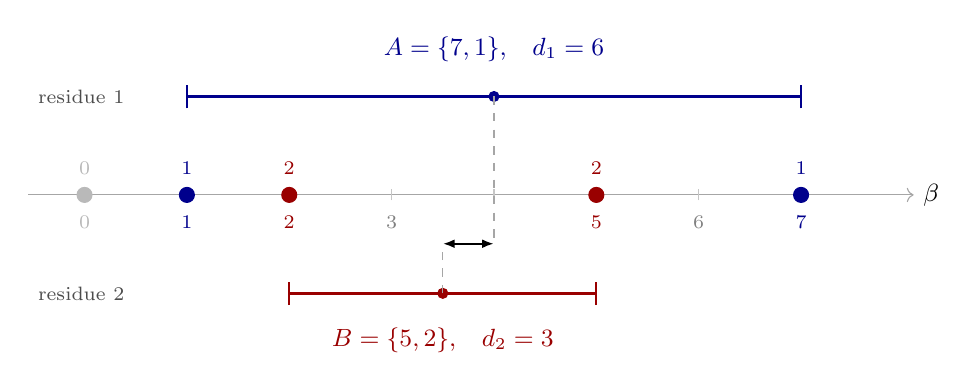
\begin{tikzpicture}[font=\small,x=1.3cm,y=1.0cm]
% --- the two intervals, well clear of the axis ---
\draw[blue!55!black,very thick] (1,1.25) -- (7,1.25);
\draw[blue!55!black,thick] (1,1.10) -- (1,1.40);
\draw[blue!55!black,thick] (7,1.10) -- (7,1.40);
\filldraw[blue!55!black] (4,1.25) circle (1.8pt);
\node[blue!55!black,above=9pt] at (4,1.25) {$A=\{7,1\}$,\quad $d_1=6$};
\draw[red!60!black,very thick] (2,-1.25) -- (5,-1.25);
\draw[red!60!black,thick] (2,-1.40) -- (2,-1.10);
\draw[red!60!black,thick] (5,-1.40) -- (5,-1.10);
\filldraw[red!60!black] (3.5,-1.25) circle (1.8pt);
\node[red!60!black,below=9pt] at (3.5,-1.25) {$B=\{5,2\}$,\quad $d_2=3$};
% --- the beta line ---
\draw[->,gray!70] (-0.55,0) -- (8.1,0) node[right,black]{$\beta$};
\foreach \b in {0,...,7} \draw[gray!45] (\b,-0.07) -- (\b,0.07);
\foreach \b in {3,6} \node[gray,font=\scriptsize,below=4pt] at (\b,0) {$\b$};
\foreach \b/\c/\r in {7/blue!55!black/1, 5/red!60!black/2, 2/red!60!black/2,
                      1/blue!55!black/1, 0/gray!55/0}
  {\filldraw[\c] (\b,0) circle (2.7pt);
   \node[\c,font=\scriptsize,below=4pt] at (\b,0) {$\b$};
   \node[\c,font=\scriptsize,above=4pt] at (\b,0) {$\r$};}
% --- the centres and their distance ---
\draw[gray!70,dashed] (4,1.25) -- (4,-0.62);
\draw[gray!70,dashed] (3.5,-1.25) -- (3.5,-0.62);
\draw[{Latex[length=1.5mm]}-{Latex[length=1.5mm]},thick] (3.5,-0.62) -- (4,-0.62);
\node[font=\scriptsize,gray!60!black,anchor=west] at (-0.55,1.25) {residue $1$};
\node[font=\scriptsize,gray!60!black,anchor=west] at (-0.55,-1.25) {residue $2$};
\end{tikzpicture}
\caption{The mechanism for $t=3$, $\lambda=(3,2)$: here $N=5$, $\beta=(7,5,2,1,0)$ with residues
$(1,2,2,1,0)$ modulo $3$, so no class is empty and two classes have size two. The three arguments of
\eqref{eq:main} are the two interval lengths and twice the distance between the interval centres;
the short double arrow marks that distance, here $\tfrac12$, so that $d_3=1$.}
\label{fig:intervals}
\end{figure}

\begin{example}
For $t=3$, $\lambda=(3,2)$ as in Figure \ref{fig:intervals}, $(d_1,d_2,d_3)=(6,3,1)$ and
\[
\Phi_3\bigl((3,2);z\bigr)=\varepsilon\,
\frac{\sinh(3\theta)\sinh(\theta/2)}{\sinh(3\theta/2)\sinh\theta}.
\]
For $t=3$, $\lambda=(3,1)$ the profile is the size-three one, $(d_1,d_2,d_3)=(3,3,6)$ and
$\Phi_3=\varepsilon\,\chi_2(z)$. For $t=4$, $\lambda=(1,1,1)$ we have $\beta=(6,5,4,2,1,0)$, the
class $3$ is empty and $\Phi_4=0$.
\end{example}

\subsection{The image of the map}
Theorem \ref{thm:main} sends every partition with at most $N$ rows to three integers, so the whole
family collapses onto a sparse subset of $\ZZ^3$. By Proposition \ref{prop:quotient} the first two
coordinates are multiples of $t$; the third is not a multiple of $t$ except in the size-three
profile, where $d_3=d_1+d_2$. Figure \ref{fig:image} shows the image for $t=3$ and $t=4$, coloured
by the number of partitions collapsing onto each point.

\begin{figure}[t]
\centering
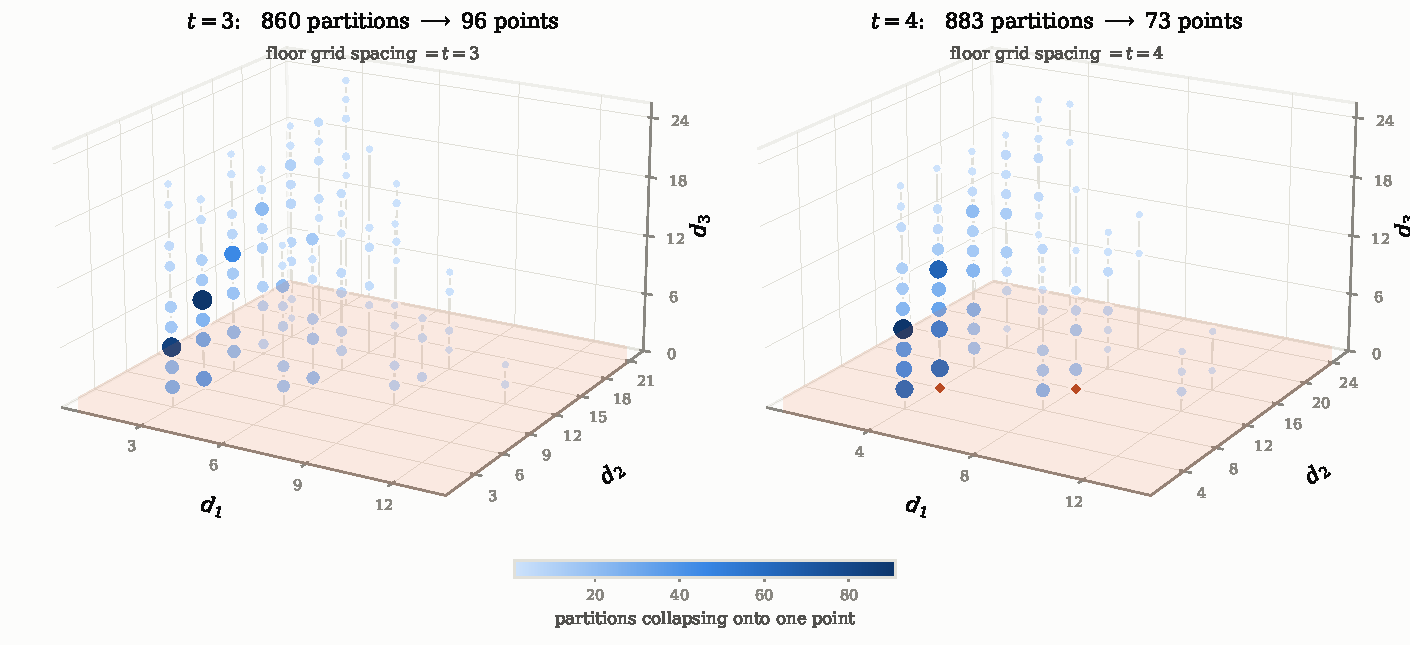
\includegraphics[width=\textwidth]{fig_image.pdf}
\caption{The image of $\lambda\mapsto(d_1,d_2,d_3)$ over all $\lambda$ with $|\lambda|\le20$ and at
most $t+2$ rows, for $t=3$ (left) and $t=4$ (right), taken \emph{up to the exchange of $d_1$ and
$d_2$}, under which \eqref{eq:main} is symmetric; without that identification, and with $A$ and $B$
in the order $r_A\le r_B$ of Theorem \ref{thm:main}, the two panels carry $126$ and $92$ points
rather than $96$ and $73$. The compression is the point of the picture: $860$
partitions land on $96$ triples on the left and $883$ on $73$ on the right, and colour and area give
the number of partitions mapping to each. The floor grid spacing is $t$, since $d_1,d_2\in t\ZZ$ by Proposition
\ref{prop:quotient}; the shaded plane $d_3=0$ is the concentric locus of Corollary \ref{cor:zero},
where $s_\lambda$ vanishes, so those shapes are not in the image and are drawn on the plane as
diamonds instead. The two panels are the two parities, which is the content of Proposition
\ref{rem:lattice}: the odd one carries no diamond, and can carry none; the even one carries two,
between them the images of $32$ partitions.}
\label{fig:image}
\end{figure}

Figure \ref{fig:image} is one half of the picture: it shows which triples occur, not what a triple
hides. Figure \ref{fig:fibres} is the other half. Over each cell of the $(d_1,d_2)$ floor it stands
the column of sizes $|\lambda|$ that land there, so a column is a set of partitions of different
sizes on which $\Phi_t$ takes one and the same value --- and the columns do not thin out as
$|\lambda|$ grows, since the values are confined to a lattice and the partitions are not. The most
visible one is the fibre of the empty partition: at $t=3$ the invariant $I_3=(3,3,2,+1)$ is shared by
$26$ partitions, of $19$ different sizes between $0$ and $20$, so $\Phi_3$ does not distinguish
$\varnothing$ from a shape of twenty boxes.

\begin{figure}[!ht]
\centering
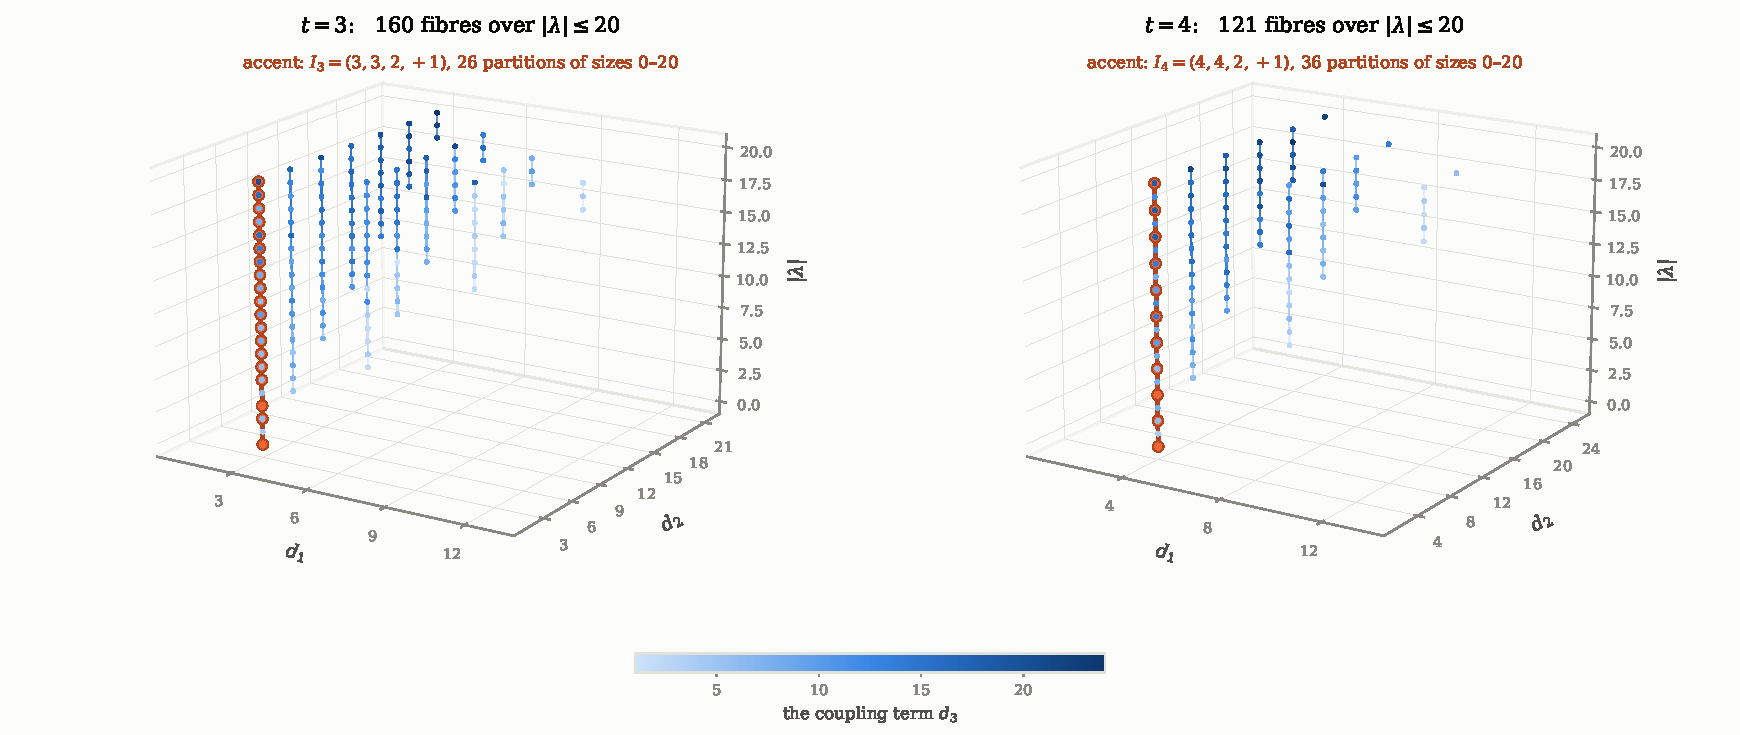
\includegraphics[width=\textwidth]{fig_fibres.pdf}
\caption{The fibres of the evaluation invariant \eqref{eq:invariant}, the complement of Figure
\ref{fig:image}: the same range $|\lambda|\le20$, with the coupling term moved to colour and the
size $|\lambda|$ on the vertical axis. A column is one fibre, so its height is the range of sizes
this alphabet cannot tell apart; the floor ticks are the lattice $t\ZZ$ of Proposition
\ref{prop:quotient}, and only the half $d_1\le d_2$ is occupied because the triple is taken up to the
exchange, as in Figure \ref{fig:image}. That every marker of a column carries the same value is
computed and not assumed: over the $860$ partitions on the left and the $883$ on the right the
bialternant is constant on each fibre to $10^{-37}$. The accent column is the fibre of
$\lambda=\varnothing$.}
\label{fig:fibres}
\end{figure}

Figure \ref{fig:fibres} makes one thing about \eqref{eq:invariant} precise: $I_t$ is complete but
not minimal. The numerator of \eqref{eq:main} is symmetric in $d_1,d_2,d_3$, so the value sees only the multiset
$\{d_1,d_2,d_3\}$ together with the sign, and that is a real reduction --- over $t=4$ and
$|\lambda|\le20$ the $121$ invariants take only $110$ values, while at $t=3$ in the same range the
two counts agree. In the same range no two distinct multisets share a value, so the minimal invariant
of this evaluation is the pair (multiset, sign); we keep the ordered form in \eqref{eq:invariant}
because $d_3$ is the coordinate the reciprocal pair contributes and the other two are not, and
Corollary \ref{cor:fibregf} describes the fibres of either, since the two differ by a symmetry of
the numerator and not by anything the lattice sees.

\begin{proposition}[a shorter form of the sign]\label{rem:sign}
Let the residue profile be non-degenerate and $a_1+a_2\ne b_1+b_2$, and order the two distinguished
classes so that $r_A\le r_B$. Then
\begin{equation}\label{eq:shortsign}
\boxed{\;\;\varepsilon_\lambda\;=\;(-1)^{\lfloor t/2\rfloor}\,\sgn(\sigma)\,(-1)^{\,r_A+r_B}\,
\sgn\bigl(a_1+a_2-b_1-b_2\bigr)\;\;}
\end{equation}
where $\sigma$ is the permutation of \S\ref{sec:background}.
\end{proposition}

\begin{proof}
Let $w$ be the residue word of $\beta(\lambda)$ read in increasing column order. Since $\beta$
decreases with the column index, grouping the parts by class with the values decreasing inside each
class is the stable sort of $w$, so $\sgn(\sigma)=(-1)^{\inv(w)}$. Both sides of
\eqref{eq:shortsign} carry the factor $\sgn(a_1+a_2-b_1-b_2)$, and
$\sgn(a_1-b_1)=(-1)^{[a_1<b_1]}$, so by \eqref{eq:sign} the assertion is equivalent to
\begin{equation}\label{eq:signparity}
j_{A_1}+j_{B_1}+\inv(w)+\inv(b_S)+[a_1<b_1]\;\equiv\;
\Bigl\lfloor\tfrac t2\Bigr\rfloor+t+\binom{N+1}{2}+r_A+r_B \pmod 2 .
\end{equation}

We use one parity count. Let $u$ be a word, $p$ a position, $c=u_p$, and let $I(p)$ be the number of
inversions of $u$ in which $p$ takes part; write $\nu_{<c}$ for the number of letters of $u$ strictly
below $c$ and $e_p$ for the number of occurrences of $c$ strictly before $p$. Putting
$x=\#\{j<p:u_j>c\}$, the positions before $p$ split as $p-1=x+e_p+\#\{j<p:u_j<c\}$ and the letters
below $c$ split as $\nu_{<c}=\#\{j<p:u_j<c\}+\#\{j>p:u_j<c\}$, whence
\begin{equation}\label{eq:parity}
I(p)\;=\;x+\#\{j>p:u_j<c\}\;=\;2x+e_p+\nu_{<c}-(p-1)\;\equiv\;(p-1)+\nu_{<c}+e_p \pmod 2 .
\end{equation}
Since $b_S$ is $w$ with the letters at the positions $j_{A_1}$ and $j_{B_1}$ deleted,
\[
\inv(w)-\inv(b_S)=I(j_{A_1})+I(j_{B_1})
-\bigl[\,\{j_{A_1},j_{B_1}\}\ \text{is an inversion of }w\,\bigr],
\]
and $\inv(w)+\inv(b_S)\equiv\inv(w)-\inv(b_S)$, so \eqref{eq:parity} computes the left-hand side of
\eqref{eq:signparity}.

In the two-class profile $r_A<r_B$, and $w$ carries $r_A$ twice, $r_B$ twice and every other residue
once. Because $\beta$ decreases with the column index, $a_1>a_2$ puts $j_{A_1}$ at the \emph{first}
occurrence of $r_A$, so $e=0$ there, and likewise at $j_{B_1}$. The letters below $r_A$ are one copy
of each of $0,\dots,r_A-1$, so $\nu_{<r_A}=r_A$; those below $r_B$ are the same together with the
second copy of $r_A$, so $\nu_{<r_B}=r_B+1$. The two positions form an inversion exactly when the
larger letter comes first, that is when $j_{B_1}<j_{A_1}$, that is when $a_1<b_1$. Hence
\[
\inv(w)-\inv(b_S)\;\equiv\;(j_{A_1}-1+r_A)+(j_{B_1}-1+r_B+1)+[a_1<b_1]
\;\equiv\;j_{A_1}+j_{B_1}+r_A+r_B+1+[a_1<b_1],
\]
and substituting this in \eqref{eq:signparity} cancels the columns and $[a_1<b_1]$ in pairs, leaving
$\lfloor t/2\rfloor+t+\binom{N+1}{2}\equiv1$.

In the size-three profile $r_A=r_B=:r$ and the class $\{p>q>p'\}$ sits at columns $j_1<j_2<j_3$ with
$A=\{p,q\}$ and $B=\{q,p'\}$, so $j_{A_1}=j_1$ and $j_{B_1}=j_2$ carry the same letter $r$, with
$e=0$ and $e=1$ respectively and $\nu_{<r}=r$ in both; two equal letters are not an inversion, and
$a_1>b_1$. So $\inv(w)-\inv(b_S)\equiv j_1+j_2+1$, which is the displayed expression again because
$r_A+r_B=2r$ and $[a_1<b_1]=0$, and \eqref{eq:signparity} reduces to the same congruence.

Finally $N=t+2$, so that congruence reads $\lfloor t/2\rfloor+t+\binom{t+3}{2}\equiv1$: for $t=2m$
its three terms are $m$, $0$ and $m+1$, and for $t=2m+1$ they are $m$, $1$ and $m$. Both sums are
odd, and the identity holds for every $t\ge2$.
\end{proof}

The ordering by residue is not a convenience, and it is worth saying why. Exchanging the two blocks
negates the sign $\kappa_{11}$ of Lemma \ref{lem:L4} --- through its $\sgn(a_1-b_1)$ factor --- and negates
$\sgn(a_1+a_2-b_1-b_2)$ as well, so it leaves $\varepsilon_\lambda$, which is their product,
invariant; as it must, since $\varepsilon_\lambda$ is attached to $\lambda$. The right-hand side
above is \emph{not} invariant: $(-1)^{r_A+r_B}$ is symmetric, so only its last factor changes sign.
Without a rule fixing which block is $A$, the right-hand side is therefore not a function of
$\lambda$ at all. The hypothesis enters the proof at one point and one only: it is what makes
$\nu_{<r_A}=r_A$ and $\nu_{<r_B}=r_B+1$ rather than the other way round, and dropping it exchanges
those two counts and breaks \eqref{eq:signparity}.

Read the other way round, \eqref{eq:shortsign} says that $\Phi_t$ is a function of a small
combinatorial datum and of nothing else, and it says so for every $t$ rather than over a range: by
Theorem \ref{thm:main} the triple $(d_1,d_2,d_3)$ determines $\Phi_t$ up to sign, and adjoining
$\sgn(\sigma)$, the ordered pair $r_A\le r_B$ and the \emph{orientation}
$\sgn(a_1+a_2-b_1-b_2)$ of $d_3$ determines it outright. The shape of $\lambda$ enters nowhere else.
The orientation is not optional, and that part remains a check rather than a proof: over $t\le6$ and
$|\lambda|\le14$, putting $\sgn(a_1-b_1)$ in its place leaves collisions at $t=2$.

%======================================================================
\section{Proof of Theorem \ref{thm:main}}\label{sec:proof}

The proof uses the Vandermonde determinant, the Laplace expansion, and one cancellation lemma. We
give the steps separately so that a reader checking the ancillary scripts can localise any
disagreement.

What the argument really does is classify rather than compute. Expanding along the $t$ frozen rows
leaves one term for each way of choosing which two columns are \emph{not} frozen, and the excess-two
count says every such choice falls into exactly one of three combinatorial types: none survives
(a residue class is empty), four survive (two classes of size two), or three do (one class of size
three). Everything after that is bookkeeping inside a type, and Lemma \ref{lem:L5} shows the last two
types are one statement seen twice.

\begin{lemma}\label{lem:L1}
Let $S$ be a set of $t$ columns and $M_S=\det(\zeta^{k\beta_j})_{0\le k<t,\,j\in S}$. Then $M_S=0$
unless the residues $\{\beta_j\bmod t:j\in S\}$ are pairwise distinct, in which case
$M_S=(-1)^{\inv(b_S)}V$.
\end{lemma}

\begin{proof}
Since $\zeta^{k\beta_j}=(\zeta^{\beta_j})^k$, the matrix is a Vandermonde matrix in the values
$y_j=\zeta^{\beta_j}$, whose determinant is $\prod_{j<j'}(y_{j'}-y_j)$. The value $y_j$ depends on
$\beta_j$ only modulo $t$, so two columns of $S$ sharing a residue make the determinant vanish. If
the residues are pairwise distinct then $|S|=t$ forces $\{y_j\}_{j\in S}=\zt$ as a set, and the
Vandermonde determinant is alternating in its arguments, so it equals $V$ times the sign of the
permutation sorting $b_S$ increasingly, which is $(-1)^{\inv(b_S)}$.
\end{proof}

\begin{lemma}\label{lem:L2}
$\det\bigl(x_i^{N-j}\bigr)_{i,j=1}^{N}
=(-1)^{\binom t2}\,V\,(z^t-1)(z^{-t}-1)(z-z^{-1})$ for the alphabet
$x=(1,\zeta,\dots,\zeta^{t-1},z,z^{-1})$ in that order.
\end{lemma}

\begin{proof}
The determinant is $\prod_{i<i'}(x_i-x_{i'})$. Pairs inside $\zt$ contribute
$\prod_{k<k'}(\zeta^k-\zeta^{k'})=(-1)^{\binom t2}V$; pairs $(\zeta^k,z)$ contribute
$\prod_k(\zeta^k-z)=(-1)^t(z^t-1)$ and pairs $(\zeta^k,z^{-1})$ contribute $(-1)^t(z^{-t}-1)$; the
last pair contributes $z-z^{-1}$. The two factors $(-1)^t$ cancel.
\end{proof}

\begin{lemma}\label{lem:L3}
Let $\mathcal U$ be the set of pairs $U=\{j_1<j_2\}$ of columns whose complement $S_U$ carries all
$t$ residues. Then
\[
\Phi_t(\lambda;z)=\frac{(-1)^{\,t+\binom{N+1}{2}}}{(z^t-1)(z^{-t}-1)(z-z^{-1})}
\sum_{U\in\mathcal U}(-1)^{\,j_1+j_2+\inv(b_{S_U})}\,f(\beta_{j_1}-\beta_{j_2}).
\]
\end{lemma}

\begin{proof}
Expanding the numerator by Laplace along the first $t$ rows,
\[
\det\bigl(x_i^{\beta_j}\bigr)=\sum_{|S|=t}(-1)^{\binom{t+1}{2}+\sum_{j\in S}j}\,M_S\,C_{S^c},
\]
where for $S^c=\{j_1<j_2\}$ the complementary $2\times2$ minor is
$z^{\beta_{j_1}-\beta_{j_2}}-z^{-(\beta_{j_1}-\beta_{j_2})}=f(\beta_{j_1}-\beta_{j_2})$. By Lemma
\ref{lem:L1} only $S$ with pairwise distinct residues contribute. Writing
$\sum_{j\in S}j=\binom{N+1}{2}-j_1-j_2$ and dividing by Lemma \ref{lem:L2}, the factors $V$ cancel
and $(-1)^{\binom{t+1}{2}-\binom{t}{2}}=(-1)^t$.
\end{proof}

If some $n_i=0$ then no $S$ of size $t$ carries all residues, $\mathcal U=\varnothing$, and
$\Phi_t=0$: this is Theorem \ref{thm:main}(i). Otherwise all $n_i\ge1$ and by \eqref{eq:excess}
either two classes have size two, in which case $S_U$ must drop one element of each and
$|\mathcal U|=4$, or one class has size three, in which case $S_U$ drops two of the three and
$|\mathcal U|=3$.

\begin{lemma}[the column move]\label{lem:L4}
Let $A$ and $B$ be distinct classes of size two, at columns $j_{A_1}<j_{A_2}$ and
$j_{B_1}<j_{B_2}$. For $i,j\in\{1,2\}$ let $U_{ij}$ consist of the column of $a_i$ and the column of
$b_j$, and set $\kappa_{ij}=(-1)^{\,j_{A_i}+j_{B_j}+\inv(b_{S_{U_{ij}}})}\sgn(a_i-b_j)$, so that
the $U_{ij}$ term of Lemma \ref{lem:L3} equals $\kappa_{ij}f(a_i-b_j)$. Then
$\kappa_{ij}=\kappa_{11}(-1)^{i-1}(-1)^{j-1}$.
\end{lemma}

\begin{proof}
Fix $j$ and compare $i=1$ with $i=2$. The sets $S_{U_{1j}}$ and $S_{U_{2j}}$ differ only in that the
first contains the column $j_{A_2}$ and the second the column $j_{A_1}$, and the letter carried is
the residue $r_A$ in both. Passing from one word to the other moves that letter across exactly the
kept columns strictly between $j_{A_1}$ and $j_{A_2}$, and none of those letters equals $r_A$
because the class $A$ has only two elements; each crossing changes the parity of $\inv$. Hence
\[
(-1)^{\inv(b_{S_{U_{1j}}})-\inv(b_{S_{U_{2j}}})}
=(-1)^{(j_{A_2}-j_{A_1}-1)-[\,a_2<b_j<a_1\,]},
\]
using that $\beta$ is strictly decreasing in the column index, so that $j_{B_j}$ lies strictly
between $j_{A_1}$ and $j_{A_2}$ exactly when $a_2<b_j<a_1$. Multiplying by the Laplace factor
$(-1)^{j_{A_1}+j_{A_2}}$,
\[
\frac{\kappa_{1j}}{\kappa_{2j}}
=(-1)^{2j_{A_2}-1}(-1)^{[\,a_2<b_j<a_1\,]}\sgn(a_1-b_j)\sgn(a_2-b_j)=-1,
\]
because $\sgn(a_1-b_j)\sgn(a_2-b_j)=-1$ exactly when $b_j$ lies between $a_2$ and $a_1$. Exchanging
the roles of $A$ and $B$ gives $\kappa_{i1}/\kappa_{i2}=-1$.
\end{proof}

\begin{lemma}\label{lem:L5}
For all $c,p,q$ and all $u,v$,
\begin{align*}
\text{\rm(a)}&\quad \sum_{\epsilon,\eta\in\{\pm1\}}\epsilon\eta\,f(c+\epsilon p+\eta q)=f(c)f(p)f(q),\\
\text{\rm(b)}&\quad f(2u)-f(2u+2v)+f(2v)=-f(u)f(v)f(u+v).
\end{align*}
\end{lemma}

\begin{proof}
For (a), $\sum_{\epsilon,\eta}\epsilon\eta\,z^{c+\epsilon p+\eta q}
=z^{c}\bigl(\sum_\epsilon\epsilon z^{\epsilon p}\bigr)\bigl(\sum_\eta\eta z^{\eta q}\bigr)
=z^{c}f(p)f(q)$, and the same computation for the negative exponents gives
$z^{-c}(-f(p))(-f(q))$; subtract. For (b), put $s=z^u$, $w=z^v$ and expand
$(s-s^{-1})(w-w^{-1})(sw-s^{-1}w^{-1})$: the eight terms recombine as
$(s^2w^2-s^{-2}w^{-2})-(s^2-s^{-2})-(w^2-w^{-2})=f(2u+2v)-f(2u)-f(2v)$.
\end{proof}

\begin{proof}[Proof of Theorem \ref{thm:main}]
In the two-class profile, Lemmas \ref{lem:L3} and \ref{lem:L4} give
\[
\sum_{U\in\mathcal U}(\cdots)=\kappa_{11}\sum_{i,j}(-1)^{i-1}(-1)^{j-1}f(a_i-b_j).
\]
Writing $a_i=\alpha+\epsilon_ip$ and $b_j=\gamma+\eta_jq$ with $p=d_1/2$, $q=d_2/2$ and
$\epsilon=\eta=(+1,-1)$, we have $a_i-b_j=c+\epsilon_ip-\eta_jq$ with $c=\alpha-\gamma$. Replacing
$\eta$ by $-\eta$ turns the sum into $-\sum_{\epsilon,\eta}\epsilon\eta f(c+\epsilon p+\eta q)$,
which is $-f(c)f(p)f(q)$ by Lemma \ref{lem:L5}(a). Since
$(z^t-1)(z^{-t}-1)=2-z^t-z^{-t}=-f(t/2)^2$ and $z-z^{-1}=f(1)$, the two minus signs cancel, and
substituting $f(u)=2\sinh(u\theta)$ the numerical factors cancel and
$\sinh(c\theta)=\sgn(c)\sinh(d_3\theta/2)$, giving \eqref{eq:main} with
$\varepsilon_\lambda=(-1)^{\,t+\binom{N+1}{2}}\kappa_{11}\sgn(a_1+a_2-b_1-b_2)$, which is
\eqref{eq:sign} by the definition of $\kappa_{11}$ in Lemma \ref{lem:L4}.

For the size-three profile $\{p>q>r\}$ at columns $j_1<j_2<j_3$ the same column-move argument
applies, again because no letter strictly between two of these columns carries the class residue,
and gives alternating signs $(\varsigma,-\varsigma,\varsigma)$ for the three terms $f(p-q)$,
$f(p-r)$, $f(q-r)$. By Lemma \ref{lem:L5}(b) with $u=(p-q)/2$, $v=(q-r)/2$ the sum is
$-\varsigma f(u)f(v)f(u+v)$, which is the two-class formula for $A=\{p,q\}$, $B=\{q,r\}$ with
$\varsigma=\kappa_{11}$. Equivalently, the missing fourth selection of the two-class profile would
drop $q$ twice and its term carries $f(0)=0$, so the two profiles are one statement.
\end{proof}

All the statements of this paper were also checked numerically; the counts are collected once, in
\S\ref{sec:verif}, rather than repeated as they arise.

%======================================================================
\section{Independence on the reciprocal locus}\label{sec:independence}

Specializing \eqref{eq:AK53} as in \S\ref{sec:background} gives: for $\ell(\lambda)\le2$,
$s_\lambda(z,\zb,\zt)=s_\lambda(z,\zb)$ if and only if $\lambda=\core_t(\lambda)$. Theorem
\ref{thm:main} evaluates the left-hand side for every $\lambda$, and comparing the two shows that on
the reciprocal locus the criterion acquires further solutions --- exactly one family.

We first isolate when $\Phi_t$ degenerates to a single character. Recall
$\chi_k(z)=(z^{k+1}-z^{-k-1})/(z-z^{-1})$.

\begin{lemma}\label{lem:single}
$\Phi_t(\lambda;z)=\pm\chi_k(z)$ for some $k\ge0$ if and only if the multiset $\{d_1,d_2,d_3\}$
contains $t$ at least twice, and in that case the remaining entry equals $2(k+1)$.
\end{lemma}

\begin{proof}
Put $u=z^{1/2}$, so that $2\sinh(d_i\theta/2)=u^{d_i}-u^{-d_i}$, $2\sinh(t\theta/2)=u^{t}-u^{-t}$ and
$2\sinh\theta=u^{2}-u^{-2}$; all exponents are integers. By \eqref{eq:main}, the asserted equality is
\[
\prod_{i=1}^{3}\bigl(u^{d_i}-u^{-d_i}\bigr)
=\pm\bigl(u^{t}-u^{-t}\bigr)^{2}\bigl(u^{2k+2}-u^{-2k-2}\bigr).
\]
Using $u^{n}-u^{-n}=u^{-n}(u^{2n}-1)$ on each factor and comparing the monomial prefactors gives
$d_1+d_2+d_3=2t+2(k+1)$ together with
\[
\prod_{i=1}^{3}\bigl(u^{2d_i}-1\bigr)=\pm\bigl(u^{2t}-1\bigr)^{2}\bigl(u^{4(k+1)}-1\bigr),
\]
and evaluating at $u=0$ fixes the sign to $+$. Now $u^{2n}-1=\prod_{m\mid 2n}\Phi_m(u)$ with
$\Phi_m$ the cyclotomic polynomials, which are irreducible and pairwise distinct, so by unique
factorization in $\ZZ[u]$ the two sides have the same multiset of cyclotomic factors. On the left
that multiset is $\biguplus_i\{m:m\mid 2d_i\}$ and on the right it is
$2\times\{m:m\mid 2t\}\uplus\{m:m\mid 4(k+1)\}$. Its largest element is $\max_i 2d_i$ on the left and
$\max(2t,4(k+1))$ on the right; deleting the divisor set of that maximum from both sides and
repeating twice more yields
\[
\{2d_1,2d_2,2d_3\}=\{2t,\,2t,\,4(k+1)\}
\]
as multisets, which is the assertion. The converse is the same computation read backwards.
\end{proof}

\begin{theorem}\label{thm:extra}
Let $\ell(\lambda)\le2$. Then $\Phi_t(\lambda;z)=\pm s_\lambda(z,\zb)$ if and only if either
$\lambda=\core_t(\lambda)$, or
\begin{equation}\label{eq:extra}
t\ \text{is even}\quad\text{and}\quad \lambda=\Bigl(\lambda_2+\tfrac{3t}{2}-1,\ \lambda_2\Bigr)
\quad\text{with}\quad \tfrac t2\le\lambda_2\le t-1 .
\end{equation}
In the second case $\{d_1,d_2,d_3\}=\{3t,t,t\}$, while $\core_t(\lambda)=\bigl(\tfrac t2-1+j,j\bigr)$
and $\quot_t(\lambda)$ has the single nonempty component $(2)$, in slot $j=\lambda_2-\tfrac t2$.
\end{theorem}

Figure \ref{fig:locus} is the statement computed rather than asserted: both families are plotted
over a range of $t$, and the odd $t$ where \eqref{eq:extra} cannot occur is drawn as the control.

\begin{figure}[!ht]
\centering

\includegraphics[width=\textwidth]{fig_locus.pdf}
\caption{Theorem \ref{thm:extra}, computed rather than asserted. For every two-row $\lambda$ in
range, both sides of $\Phi_t(\lambda;z)=\pm s_\lambda(z,\zb)$ were evaluated; the partitions where
they agree are plotted and coloured by family. Circles are the $t$-cores, the solutions already
described by \eqref{eq:AK53}; triangles are the extra family \eqref{eq:extra}, which the reciprocal
specialization creates. The odd case $t=3$ is the control: by Theorem \ref{thm:extra} no extra
solution can exist there, and none is found.}
\label{fig:locus}
\end{figure}

\begin{proof}
Since $\ell(\lambda)\le 2$ and $N=t+2$, the beta set is
$\beta(\lambda)=\bigl(A'+t,\;B'+t,\;t-1,t-2,\dots,1,0\bigr)$ where
\[
A':=\lambda_1+1,\qquad B':=\lambda_2,\qquad A'>B'\ge0 .
\]
The block $\{0,1,\dots,t-1\}$ meets every residue class exactly once, so no class is empty and the
two large parts decide the profile. Write $A'=t\alpha+\rho_A$ and $B'=t\gamma+\rho_B$ with
$0\le\rho_A,\rho_B\le t-1$. As $s_\lambda(z,\zb)=\chi_{\lambda_1-\lambda_2}(z)$, Lemma
\ref{lem:single} says that the assertion holds precisely when $\{d_1,d_2,d_3\}$ contains $t$ twice
and the third entry is $2(\lambda_1-\lambda_2+1)=2(A'-B')$.

\emph{Case $\rho_A=\rho_B=:\rho$.} One class has size three, namely $\{A'+t,B'+t,\rho\}$, and by
Theorem \ref{thm:main} the three arguments are
$d_1=A'-B'$, $d_2=B'+t-\rho=t(\gamma+1)$, $d_3=A'+t-\rho=t(\alpha+1)$. Here $t\mid A'-B'$, say
$A'-B'=ts$ with $s\ge1$. The pair $d_2=d_3=t$ forces $\alpha=\gamma=0$, hence $A'=B'$, excluded.
The pair $d_1=d_3=t$ forces $s=1$ and $\alpha=0$, hence $A'<t$ and $A'=B'+t\ge t$, excluded. The pair
$d_1=d_2=t$ forces $s=1$ and $\gamma=0$, i.e. $A'=B'+t$ with $B'<t$; then $\alpha=1$ and the third
entry is $d_3=2t=2(A'-B')$, as required. So this case contributes exactly the $\lambda$ with
$A'=B'+t$, $B'<t$.

\emph{Case $\rho_A\ne\rho_B$.} Two classes have size two, namely $\{A'+t,\rho_A\}$ and
$\{B'+t,\rho_B\}$, and the three arguments are
\[
d_A=t(\alpha+1),\qquad d_B=t(\gamma+1),\qquad
d_3=\bigl|\,t(\alpha-\gamma)+2(\rho_A-\rho_B)\,\bigr| .
\]
If $d_A=d_B=t$ then $\alpha=\gamma=0$, so $A',B'<t$ and $d_3=2|\rho_A-\rho_B|=2(A'-B')$
automatically: every such $\lambda$ is a solution. Otherwise exactly one of $d_A,d_B$ equals $t$ and
$d_3=t$. If $\alpha=0$ and $\gamma\ge1$ then $|-t\gamma+2(\rho_A-\rho_B)|=t$ with
$|\rho_A-\rho_B|\le t-1$ forces $\gamma=2$ and $\rho_A-\rho_B=t/2$; but then
$\lambda_1=A'-1=\rho_A-1<t$ while $\lambda_2=B'\ge2t$, contradicting $\lambda_1\ge\lambda_2$. If
$\gamma=0$ and $\alpha\ge1$ then $|t\alpha+2(\rho_A-\rho_B)|=t$ forces, for $\alpha=1$,
$\rho_A=\rho_B$ (excluded), and for $\alpha=2$,
\[
\rho_B-\rho_A=\tfrac t2,
\]
which requires $t$ even; $\alpha\ge3$ gives $|2(\rho_A-\rho_B)|\ge2t$, impossible. So $A'=2t+\rho_A$,
$B'=\rho_B=\rho_A+\tfrac t2$, whence
\[
\lambda_1=2t+\rho_A-1,\qquad \lambda_2=\rho_A+\tfrac t2,\qquad
\lambda_1-\lambda_2=\tfrac{3t}{2}-1,
\]
and $\rho_B\le t-1$ gives $0\le\rho_A\le\tfrac t2-1$, i.e. $\tfrac t2\le\lambda_2\le t-1$. The
remaining entry is $d_A=t(\alpha+1)=3t=2(\lambda_1-\lambda_2+1)$, as required. This is
\eqref{eq:extra}.

It remains to identify the solutions collected in the first case of each analysis with the
$t$-cores. For $\ell(\lambda)\le2$ the beta set in two slots is $(A',B')$, and $\lambda$ is a
$t$-core if and only if neither beta number can be lowered by $t$ into an unoccupied nonnegative
position, i.e. if and only if $B'<t$ and either $A'<t$ or $A'=B'+t$. These are exactly the two
families found above. Finally, in case \eqref{eq:extra} the class $\rho_A$ carries
$\{2t+\rho_A+t,\rho_A\}$, so its quotient component is $(2)$, every other component is empty, and
the core is as stated.
\end{proof}


\begin{remark}\label{rem:why}
Theorem \ref{thm:extra} is stated up to sign because that is what Lemma \ref{lem:single} controls;
over two-row shapes with $t\le8$ the sign is $+1$ at every solution, so there the equality holds on
the nose.

The extra family belongs to the specialization rather than to the alphabet. The step is
\cite[Lemma 5.2]{AK25}, on which \cite[Theorem 5.3]{AK25} rests: it reduces the independence to the
vanishing of $s_{\lambda/\mu}$ at the twisted alphabet for all $\mu\subsetneq\lambda$, and the
reduction uses the linear independence of the universal characters $f_\mu$ in the free variables. On the reciprocal locus $s_\mu(z,\zb)=\chi_{\mu_1-\mu_2}(z)$
depends only on $\mu_1-\mu_2$, so $s_{(1)}$, $s_{(2,1)}$ and $s_{(3,2)}$ agree there and that
independence is not available; Theorem \ref{thm:extra} measures the difference. A control confirms
the reading: for $\lambda=(3,1)$ and $t=2$ one has $s_\lambda(\zt,z,\zb)=s_\lambda(z,\zb)$, while
$s_\lambda(\zt,x,y)\ne s_\lambda(x,y)$ for free $x,y$.
\end{remark}

So the criterion does not survive the specialization unchanged, and what it acquires is small and
nameable: one family, for two-row shapes, indexed by an order-two element of the residue lattice and
classified by its core and quotient. The extra solutions belong to the reciprocal locus, not to the
alphabet --- they exist because a specialization has removed a linear independence the original
argument used, and that missing step is exactly what Theorem \ref{thm:extra} measures.

%======================================================================
\section{An enumeration in which a parameter survives}\label{sec:enum}

Expanding $s_\lambda$ over semistandard tableaux turns Theorem \ref{thm:main} into a product formula
for a weighted count. Let $m_k(T)$ be the number of entries equal to $k$ in $T$.

\begin{corollary}\label{cor:enum}
Expanding $s_\lambda$ over semistandard tableaux and applying Theorem \ref{thm:main}: for every
$t\ge2$ and every $\lambda\in\PP_{t+2}$,
\[
\sum_{T\in\mathrm{SSYT}(\lambda,\,t+2)}
\zeta^{\,\sum_{k=1}^{t}(k-1)m_k(T)}\;z^{\,m_{t+1}(T)-m_{t+2}(T)}
\;=\;\varepsilon_\lambda\,
\frac{\sinh(d_1\theta/2)\sinh(d_2\theta/2)\sinh(d_3\theta/2)}{\sinh^2(t\theta/2)\sinh\theta}.
\]
\end{corollary}

For $t=2$ the weight is $(-1)^{m_2(T)}$, and if $\lambda=(c^r)$ is rectangular then
$\mathrm{SSYT}(\lambda,4)$ is in bijection with plane partitions in an $r\times(4-r)\times c$ box,
equivalently with lozenge tilings of a hexagon. Corollary \ref{cor:enum} is then a
$(-1)$-enumeration of those objects \emph{refined by a free parameter} $z$, which records the
difference between the numbers of entries $3$ and $4$. Setting $z=1$ recovers the plain signed
count, which by \eqref{eq:main} equals $\pm d_1d_2d_3/(2t^2)$: for $r=2$, $c=2$ it is $4$; for
$r=2$, $c=4$ it is $9$; for $r=3$, $c=3$ it is $-6$.

\begin{example}\label{ex:boxes}
Taking $\lambda=(c^{\,r})$ with $1\le r\le4$ and $t=2$, the shape has at most four rows, the tableaux
are the plane partitions in an $r\times(4-r)\times c$ box, and the closed form gives the signed
counts of Figure \ref{fig:signed}. Reading it off:
\[
\begin{array}{ll}
1\times3\times c: & \bigl\lfloor (c+2)^2/4\bigr\rfloor,\\[2pt]
2\times2\times c: & (c/2+1)^2 \text{ for } c \text{ even},\qquad 0 \text{ for } c \text{ odd},\\[2pt]
3\times1\times c: & (-1)^c\bigl\lfloor (c+2)^2/4\bigr\rfloor,\\[2pt]
4\times0\times c: & (-1)^c .
\end{array}
\]
The third row is the transpose of the first, which is why the magnitudes agree; the fourth is the
degenerate box, where $s_{(c^4)}(x)=(x_1x_2x_3x_4)^c$ and the alphabet has determinant $-1$. We do
not claim these particular counts as new --- the boxes are small and the sign here is the
specialization $x_2=-1$, not the complementation sign of Kuperberg's $(-1)$-enumerations --- and we
record them only to show what the theorem produces. What does appear to be new is that each of them
is the $z\mapsto1$ value of a one-parameter refinement with the same product formula.
\end{example}

The perfect squares in Example \ref{ex:boxes} are not an accident of small cases: they are what the
interval reading of \S\ref{sec:intervals} says a rectangle must produce.

\begin{proposition}\label{prop:rect}
Let $t=2$ and $\lambda=(c^{\,r})$ with $1\le r\le4$. Then one of $d_1,d_2,d_3$ equals $2$, and:
\begin{enumerate}
\item[\rm(i)] if $r=4$, all three equal $2$ for \emph{every} $c$ and the count is $(-1)^c$; this is
the full rectangle, where $s_{(c^4)}(x)=(x_1x_2x_3x_4)^{c}$ collapses to a monomial and the alphabet
contributes only its determinant;
\item[\rm(ii)] if $r\le3$ and $c$ is even, the other two are both equal to $c+2$, so the two
intervals have the \emph{same length} and the signed count is the perfect square
$\bigl(\tfrac{c+2}{2}\bigr)^2$;
\item[\rm(iii)] if $c$ is odd and $r=2$, the two intervals are \emph{concentric} and the count is $0$;
\item[\rm(iv)] if $c$ is odd and $r\in\{1,3\}$, the other two are $c+1$ and $c+3$, and the count is
$\pm\tfrac{(c+1)(c+3)}{4}=\pm\bigl\lfloor\tfrac{(c+2)^2}{4}\bigr\rfloor$.
\end{enumerate}
Case {\rm(i)} is not a degeneration of the interval triple but a collapse of the shape itself, and it
is the only case in which the parity of $c$ plays no role.
\end{proposition}

\begin{proof}
For $\lambda=(c^{\,r})$ the beta set consists of two blocks of consecutive integers, namely
$c+3,c+2,\dots,c+4-r$ and $3-r,2-r,\dots,0$; residues alternate along each block, which is what
forces the coincidences. Explicitly, for $r=1,2,3,4$ the beta set is $(c+3,2,1,0)$, $(c+3,c+2,1,0)$,
$(c+3,c+2,c+1,0)$ and $(c+3,c+2,c+1,c)$. Splitting each by parity gives, for $c$ even,
\[
\{c{+}3,1\},\{2,0\};\qquad \{c{+}3,1\},\{c{+}2,0\};\qquad \{c{+}3,c{+}1\},\{c{+}2,0\};\qquad
\{c{+}3,c{+}1\},\{c{+}2,c\},
\]
whence $(d_1,d_2,d_3)$ equals $(c{+}2,2,c{+}2)$, $(c{+}2,c{+}2,2)$, $(2,c{+}2,c{+}2)$ and
$(2,2,2)$ respectively; in each case the product over $2t^2=8$ is $\bigl(\tfrac{c+2}{2}\bigr)^2$,
resp. $1$. For $c$ odd and $r=2$ the split is $\{c{+}3,0\},\{c{+}2,1\}$, so
$d_3=|c{+}3+0-c{-}2-1|=0$: the intervals are concentric and Corollary \ref{cor:zero} applies. For
$c$ odd and $r=1,3$ the parity puts three beta numbers in one class, $\{c{+}3,2,0\}$ and
$\{c{+}3,c{+}1,0\}$ respectively, and the size-three profile gives $(c{+}1,2,c{+}3)$ and
$(2,c{+}1,c{+}3)$, with product over $8$ equal to $\tfrac{(c+1)(c+3)}{4}$. For $c$ odd and $r=4$ the
four beta numbers are again consecutive, so the split is $\{c{+}3,c{+}1\},\{c{+}2,c\}$ and the triple
is $(2,2,2)$ exactly as for $c$ even: at full height the answer does not see the parity of $c$, which
is why $r=4$ is separated out.
\end{proof}

So the square is the square of half the common interval length, the zeros are the concentric
configurations, the quarter-squares are the case where the two lengths differ by $2$, and at full
height all three intervals coincide, the shape becomes a monomial and only a sign survives. Which
pair of the three coincides rotates with $r$, which is why the same value appears in different
columns of Figure \ref{fig:signed}.

\begin{figure}[t]
\centering

\includegraphics[width=\textwidth]{fig_signed.pdf}
\caption{The signed counts of Example \ref{ex:boxes}: the value of Corollary \ref{cor:enum} at
$z=1$ and $t=2$ for the rectangular shapes $\lambda=(c^{\,r})$, that is the $(-1)$-enumeration of
plane partitions in an $r\times(4-r)\times c$ box. Every entry is the closed form
$\varepsilon_\lambda\,d_1d_2d_3/(2t^2)$, cross-checked against a direct enumeration of the tableaux.
The row $r=2$ vanishes for odd $c$ and is a perfect square for even $c$.}
\label{fig:signed}
\end{figure}

The $(-1)$-enumeration literature --- Kuperberg \cite{Kup02}, Eisenk\"olbl \cite{Eis07} building on
Stanley \cite{Sta86} and on the Pfaffian identities of \cite{IOTZ06}, Ciucu, Krattenthaler ---
computes such signed counts with the variables specialized to $1$. Keeping the parameter free appears not to have
been recorded, and it is the feature that distinguishes the present alphabet: the reciprocal pair is
precisely the mechanism that lets one variable survive the signed enumeration.

A refinement of a different kind is standard in the ribbon world, and it is worth saying which:
the LLT polynomials of Lascoux, Leclerc and Thibon \cite{LLT97} grade ribbon tableaux by a spin
statistic. That $q$ is an extra grading rather than a letter, and the object it grades is indexed by
a tuple of shapes; the parameter here is the alphabet's own and what carries it is a single
$s_\lambda$. The two refine different things, which is why we put the point narrowly: it is the
reciprocal pair, and not a statistic, that keeps a variable alive through the signed count.

A signed enumeration with a product formula asks for a sign-reversing involution, and the obstruction
is specific: the involution must preserve $m_{t+1}-m_{t+2}$, or the free parameter is not carried
across, and neither Bender--Knuth moves nor the single-cell toggle do. The construction in
\cite{KumariThesis} of a fixed-point-free sign-reversing involution on semistandard tableaux over a
$\pm$-paired alphabet, whose fixed set is the domino-tileable tableaux, does have the required
property in its $i=1$ instance: it touches only cells holding $1$ or $2$, hence preserves
$z^{m_3-m_4}$ and reverses $(-1)^{m_2}$. The triple product it would have to land on is the one of
Corollary \ref{cor:chars}, which at $t=2$ is a product of three $\mathfrak{sl}_2$ characters on the
nose, so the missing bijection is a Clebsch--Gordan statement. That is one half. The other is the
cancellation across the
splitting of the alphabet, and at $t=2$ it concerns a single one-parameter family. By
\eqref{eq:threestep} below,
\[
s_\lambda(1,-1,z,\zb)=\sum_{\ell(\nu)\le2}s_{\lambda/\nu}(1,-1)\,\chi_{\nu_1-\nu_2}(z),
\]
and an involution carrying the parameter must preserve $k=\nu_1-\nu_2$, since that is the index of
the character its term sits on. For fixed $k$ the admissible $\nu$ are exactly $(m+k,m)$ with
$m\ge0$, so that cancellation is a statement about one word.

The size of the terms is classical. Littlewood's theorem has a skew form --- $\varphi_t
s_{\lambda/\nu}$ vanishes unless $\lambda/\nu$ is tileable by $t$-ribbons, and is otherwise a ribbon
sign times a product over the quotient --- due to Macdonald \cite[p.~91]{Mac95}, and proved there by
the same Jacobi--Trudi route we take below; the case where $\nu$ is the $t$-core is Farahat's. At
$t=2$ on our alphabet it gives $\sigma_m\in\{0,\pm1\}$ at once. What is not classical is how the
sign moves with $m$, and that is what the involution needs.

\begin{figure}[t]
\centering

\includegraphics[width=\textwidth]{fig_runs.pdf}
\caption{Proposition \ref{rem:involution}, drawn. For each $k$ the admissible $\nu$ are the single
family $(m+k,m)$, and $\sigma_m=s_{\lambda/(m+k,m)}(1,-1)$ is plotted against $m$ and $k$; the grey
dots are the zeros. Every bar has height exactly $\pm1$, which is part (i): the terms are a set, so
the cancellation the enumeration asks for is a matching and not something carrying multiplicity. On
the left every $k$ is even and the colour alternates along each run, which is part (iii) and what
makes $m\leftrightarrow m+1$ sign-reversing; where a run ends, a zero ends it. On the right every
$k$ is odd and no two nonzero terms are adjacent, which is part (ii): the runs have length one and
there is nothing to cancel.}
\label{fig:runs}
\end{figure}

\begin{proposition}[the runs alternate]\label{rem:involution}
Let $t=2$, let $k\ge0$, and put $\sigma_m=s_{\lambda/(m+k,m)}(1,-1)$ for $m\ge0$. Then
\begin{enumerate}
\item[\rm(i)] $\sigma_m\in\{0,\pm1\}$ --- this part is Macdonald's, not ours;
\item[\rm(ii)] if $k$ is odd, no two consecutive $\sigma_m$ are nonzero;
\item[\rm(iii)] if $\sigma_m$ and $\sigma_{m+1}$ are both nonzero then $\sigma_{m+1}=-\sigma_m$.
\end{enumerate}
Consequently, pairing $m$ with $m+1$ inside each maximal run of consecutive nonzero $\sigma$ is a
sign-reversing involution, and $\sum_m\sigma_m$ is the signed count of the runs of odd length.
\end{proposition}

The three parts are visible at once in Figure \ref{fig:runs}: the bar heights are part {\rm(i)}, the
gaps on the odd panel are part {\rm(ii)}, and the alternation of colour along each run is part
{\rm(iii)}.

\begin{proof}
Write $\beta_i=\lambda_i-i$ and $c_j=\nu_j-j$, and take the Jacobi--Trudi matrix of
$s_{\lambda/\nu}$ in $n\ge\ell(\lambda)$ rows. Since $h_j(1,-1)=1$ for $j\ge0$ even and $0$
otherwise,
\begin{equation}\label{eq:betaJT}
M_{ij}=\bigl[\beta_i\ge c_j\bigr]\cdot\bigl[\beta_i\equiv c_j \bmod 2\bigr],\qquad
\sigma_m=\det M .
\end{equation}
The second factor says that column $j$ is supported on the rows of one parity class, the class of
$c_j$; and since $\beta_1>\dots>\beta_n$, inside that class the first factor cuts an \emph{initial
segment}. Order the rows by parity class: $M$ becomes block diagonal, so it is singular unless each
class carries as many columns as it has rows, and inside a class it is the staircase
$\bigl[\,\text{the rank of }i\text{ in its class}\le\ell_j\bigr]$ of the segment lengths $\ell_j$. That staircase is singular if two
lengths agree or one is $0$, and otherwise the lengths are a permutation of $1,\dots,e$ and its
determinant is the sign of that permutation. This gives (i), which is \cite[p.~91]{Mac95} in this
case; we re-derive it because the $\beta$-form \eqref{eq:betaJT} is what (ii) and (iii) rest on.

For $\nu=(m+k,m)$ we have $c_1=m+k-1$, $c_2=m-2$ and $c_j=-j$ for $j\ge3$. So $c_1-c_2=k+1$, and
passing from $m$ to $m+1$ raises $c_1$ and $c_2$ by one and leaves every other column alone: exactly
the first two columns change parity class.

If $k$ is odd then $c_1\equiv c_2$, so columns $1$ and $2$ lie in the same class and both leave it.
That class's column count changes by two while its row count does not, so at most one of $\sigma_m$,
$\sigma_{m+1}$ can be nonzero, which is (ii).

If $k$ is even then $c_1\not\equiv c_2$ and the two columns exchange classes. Suppose both are
nonzero. In the class of $c_1$ the columns are column $1$ together with a set of columns $j\ge3$
that does not move; by (i) the lengths are a permutation of $1,\dots,e$ before and after, and the
fixed columns contribute the same lengths to both, so the length column $2$ brings in equals the one
column $1$ took away --- and symmetrically in the other class. Each class therefore sees the same
lengths in the same order of columns, and both block determinants are unchanged. What does change is
the shuffle separating the two classes of columns: columns $1$ and $2$ are adjacent and exchange
membership, which alters the number of inversions of that shuffle by exactly one. Hence
$\sigma_{m+1}=-\sigma_m$, which is (iii).
\end{proof}

\begin{remark}[the sign here is the sign of Theorem \ref{thm:main}]\label{rem:onesign}
Write $\sigma_\nu$ for the permutation of \S\ref{sec:background} attached to a partition $\nu$: the
one sorting $\beta$ by residue class, which Proposition \ref{rem:sign} places inside
$\varepsilon_\lambda$. The terms of Proposition \ref{rem:involution} are values of that same sign.
Indeed $\sigma_m$ vanishes unless $\core_2(\lambda)=\core_2(\nu)$ and both components of the skew
$2$-quotient are horizontal strips, and equals $\sgn(\sigma_\lambda)\sgn(\sigma_\nu)$ when it does
not --- the identity $\sgn(\sigma_\lambda)\sgn(\sigma_\nu)=(-1)^{\sum_B\mathrm{ht}(B)}$ being the
ribbon sign of \cite[p.~91]{Mac95} written as a sorting sign, which is
\cite[Lemma 6.3]{KumariThesis}. Parts {\rm(ii)} and {\rm(iii)} are
then one statement about $\sigma_\nu$ alone: as $\nu=(m+k,m)$ moves to $(m+k+1,m+1)$,
$\sgn(\sigma_\nu)$ reverses for $k$ even and is constant for $k$ odd. So the permutation that
carries the sign of the main theorem is the permutation that makes the involution of this section
alternate; the two halves of the paper are signed by one object.
\end{remark}

The pairing is a bijection of tableaux and not only of terms, which is what carries the parameter. A
semistandard tableau of shape $(a,b)$ in the letters $3,4$ has second row $4^{\,b}$ and first row
$3^{\,p}4^{\,a-p}$ with $b\le p\le a$, of weight $z^{2p-a-b}$; adjoining a first column
$\left(\begin{smallmatrix}3\\4\end{smallmatrix}\right)$ sends it to the tableau of shape
$(a+1,b+1)$ with $p+1$ in place of $p$, and $2(p+1)-(a+1)-(b+1)=2p-a-b$, so $m_3-m_4$ is preserved
exactly. Composing that with Proposition \ref{rem:involution} pairs the terms of Corollary
\ref{cor:enum} in the way the enumeration asks for.

One half is not ours, and we say which. Proposition \ref{rem:involution} disposes of the cancellation
across $\nu$; the cancellation \emph{inside} each $s_{\lambda/\nu}(1,-1)$ is
\cite{KumariThesis}, and the two fit together. There, at $n=1$, the alphabet is $(x,-x)$ and the
weight of a two-letter filling is $(-1)^{c_2}$, which is $\sigma_m$; the involution
\cite[Lemma 2.18]{KumariThesis} is fixed-point-free on the fillings that are \emph{not coverable},
so the sum reduces to the coverable ones, which \cite[Lemma 2.16]{KumariThesis} matches with domino
tableaux. What makes the reduction usable here is \cite[Lemma 2.14]{KumariThesis}: the parity of the
number of vertical dominoes does not depend on the tableau, so every survivor carries the same sign
and $\sigma_m=\pm\#\{\text{coverable fillings}\}$. With part (i) that forces the count to be at most
one, so the fixed set is a single filling when $\sigma_m\ne0$ and empty otherwise --- checked
directly over the $1134$ skew shapes with at most four rows and $|\lambda|\le10$, where the two
counts agree without exception.

At $t=2$ the involution the enumeration asks for therefore exists: cancel inside each $\nu$ by
\cite[Lemma 2.18]{KumariThesis}, pair what is left across $\nu$ by Proposition \ref{rem:involution},
and carry the parameter by the column $\left(\begin{smallmatrix}3\\4\end{smallmatrix}\right)$. Its
fixed points are one filling for each run of odd length, and Corollary \ref{cor:enum} counts them.
The construction is Kumari's; the assembly is ours.

%======================================================================
\section{The factorization is isolated}\label{sec:sharp}

A factorization is only a result if it is not a specialization of a known one, and it is only a
\emph{sharp} result if the alphabet cannot be deformed. There are four deformations of
\eqref{eq:object}, and all four destroy the product.

The evidence in this section is computational, and we label it as such: none of (D1)--(D4) below is
a theorem, and in particular we prove no no-go statement. What we assert is that the identity
\eqref{eq:main} is false for each deformed alphabet, which a single counterexample settles, and we
give counts to indicate how far from true it is.

\begin{itemize}
\item[\rm(D1)] \emph{More reciprocal pairs.} For $s_\lambda(\zt,z_1,z_1^{-1},\dots,z_r,z_r^{-1})$
with $r\ge2$ there is no product law: typical values carry one large irreducible factor, and the only
factors that split off are binomials in the rotated variables $z_1z_2$ and $z_1z_2^{-1}$, that is,
the couplings between the pairs' $u(1)$ charges. What does survive every $r$ is the \emph{zero
locus}, and Theorem \ref{thm:zeros} determines it; the product is the rank-one accident and the
vanishing is the part that generalizes.
\item[\rm(D2)] \emph{More orbit variables.} For $s_\lambda(X,\zeta X,\dots,\zeta^{t-1}X,z,z^{-1})$
with $|X|=n\ge2$ there is no product law. At $t=2$, $n=2$ the value for $\lambda=(2)$ is
$(x^2z^2+y^2z^2+z^4+z^2+1)/z^2$, irreducible over $\mathbb Q$; for $\lambda=(2,2)$ it is
$(x^2+y^2+z^2)(x^2z^2+y^2z^2+1)/z^2$, two factors rather than three; and for $\lambda=(3,1)$ it is
again irreducible. By contrast, with the pair deleted the same alphabet obeys \cite[Theorem
2.3]{AK25}: $s_{(2)}(x,y,-x,-y)=x^2+y^2$ and $s_{(2,2)}(x,y,-x,-y)=(x^2+y^2)^2$.
\item[\rm(D3)] \emph{The orbit replaced by a coset.} For $\zeta'\zt$ with $\zeta'=e^{\pi i/t}$, the
odd powers of a primitive $2t$-th root of unity --- the twist of \cite[\S3]{AK25}, and for $t$ even
the full set of primitive $2t$-th roots studied in \cite{HI24} --- the identity fails, vanishing
criterion included.
\item[\rm(D4)] \emph{The reciprocal pair replaced by a free pair.} $s_\lambda(\zt,x,y)$ is
generically irreducible.
\end{itemize}

Counts for (D3) and (D4), over $t=2,\dots,6$ and $|\lambda|\le10$: the identity holds in all $600$
cases for \eqref{eq:object}, in $383$ of $600$ for (D3), and in $200$ of $600$ for (D4). The test is
therefore capable of failing, which is the point of quoting the first row.

One reading of the proof accounts for all four. Splitting the alphabet and applying Theorem
\ref{thm:LR} to the frozen half gives, for any free alphabet $B$,
\begin{equation}\label{eq:threestep}
s_\lambda(\zt\cup B)=\sum_{\nu}s_{\lambda/\nu}(\zt)\,s_\nu(B)=\sum_\nu\varepsilon_\nu\,s_\nu(B),
\qquad \varepsilon_\nu\in\{0,\pm1\},
\end{equation}
the coefficients being ribbon signs: that the skew evaluation $s_{\lambda/\nu}(\zt)$ is $0$ or a
ribbon sign is the skew form of Theorem \ref{thm:LR}, due to Macdonald \cite[p.~91]{Mac95}. Now
$B=(z,z^{-1})$ has exactly two letters and they are
reciprocal, so $s_\nu(B)=\chi_{\nu_1-\nu_2}(z)$ is a \emph{single} $\mathfrak{sl}_2$ character
depending on one difference, and the short signed sum collapses. Step one requires the frozen half
to be a full orbit, since Theorem \ref{thm:LR} needs the rows to meet every residue class exactly;
a coset does not, which is (D3). Step two requires the free half to be exactly one reciprocal pair:
a free pair has $\det=xy$ and couples to both central charges, which is (D4), and enlarging the free
half --- by more pairs, or by more orbit variables, which enlarges $\nu$ --- makes $s_\nu(B)$ cease
to be a single character and the sum cease to collapse, which is (D1) and (D2). \emph{The four
failures are one condition seen from four sides.}

\begin{remark}
Equivalently: the reciprocal pair contributes exactly \emph{one} coupling, the cross term $d_3$,
because $\det=1$ prevents it from seeing the two central charges separately. This is why there are
three factors and not two, and Ayyer--Kumari's factorizations, which are products over quotient
components with no coupling at all, are the case where that contribution is absent.
\end{remark}

\begin{remark}[a representation-theoretic reading]\label{rem:twining}
The alphabet \eqref{eq:object} is closed under inversion, hence a torus element of $O(N)$, and its
determinant is $(-1)^{t+1}$. For even $t$ it therefore lies in the non-identity component, where a
character is a \emph{twining} character; the identity computing such characters by folding is due to
Jantzen \cite{Jantzen} and, in the form closest to this one, to Kumar--Lusztig--Prasad \cite{KLP},
the relevant folded algebra being the orbit Lie algebra. Our restriction is reducible, so it is
reached from theirs by one step of Clifford theory. We record this because Ciucu--Krattenthaler
\cite{CK09} wrote that they could not offer a representation-theoretic interpretation of their
factorizations, and \cite{AB19} and \cite{AK25} repeat that it is still missing; the reading here is
of that kind. The mechanism is entirely theirs, and the proof above does not use it. Lemma
\ref{lem:AtoSp} makes the reading concrete for the alphabet \eqref{eq:psir}, where the folded algebra
is $C_r$ and the twining character is a symplectic character on the nose.
\end{remark}

%======================================================================
\section{The zero locus survives every $r$}\label{sec:zeros}

This section is past the factorization, and reads differently from the seven before it. Those prove
statements about an identity; this one asks what is left when the identity is gone, and the answer is
a locus rather than a formula --- proved in one direction for every $r$, in the other only where we
could reach. The change of register is the subject changing, not the standard.

By (D1) the product of Theorem \ref{thm:main} does not survive a second reciprocal pair. Its
\emph{zero locus} does, and for every $r$ it has a closed form. Write
\begin{equation}\label{eq:psir}
\Psi_r(\lambda)\;:=\;s_\lambda(1,-1,z_1,\bar z_1,\dots,z_r,\bar z_r),\qquad N=2r+2,
\end{equation}
so that $\Psi_1$ is \eqref{eq:object} at $t=2$. Throughout this section $\lambda$ is padded to
exactly $N$ parts, $\beta=\beta(\lambda)$ is its beta set, and $E$ and $O$ are its even and odd
entries. Call $\lambda$ \emph{self-complementary of width $w$} if $\lambda_i+\lambda_{N+1-i}=w$ for
every $i$, in which case $w=\lambda_1+\lambda_N$. The two conditions the section is about are
\begin{equation}\label{eq:branches}
\boxed{\;\;
\underbrace{|E|\in\{0,N\}}_{\text{branch (a)}}
\qquad\qquad
\underbrace{\lambda_i+\lambda_{N+1-i}=w\ \ \text{for all }i,\ \ w\ \text{odd}}_{\text{branch (b)}}
\;\;}
\end{equation}
Branch (a) says the beta set has constant parity; branch (b) says $\lambda$ is self-complementary of
odd width, the width being $w=\lambda_1+\lambda_N$.

We state the four claims separately, because they are not proved to the same extent and a single
biconditional would hide that.

\begin{theorem}[the two branches]\label{thm:zeros}
For every $r\ge1$ and every $\lambda$: if branch {\rm(a)} or branch {\rm(b)} holds, then
$\Psi_r(\lambda)=0$.
\end{theorem}

\begin{corollary}\label{cor:sizes}
If $\lambda$ is self-complementary of odd width $w$ then $|\lambda|=w(r+1)$. In particular branch
{\rm(b)} occurs only for $|\lambda|\equiv r+1 \pmod{2(r+1)}$, and a size outside that progression
needs no further test.
\end{corollary}

\begin{proof}
Summing $\lambda_i+\lambda_{N+1-i}=w$ over $i$ counts $|\lambda|$ twice, so $2|\lambda|=wN=w(2r+2)$.
\end{proof}

The progression is visible in Figure \ref{fig:zeros}, and it is worth recording that the analogous
statement for the whole locus is false: branch (a) is not confined to it, which is why the condition
has to be read off branch (b) alone.

\begin{figure}[!ht]
\centering

\includegraphics[width=\textwidth]{fig_zeros.pdf}
\caption{The zero locus of Theorem \ref{thm:zeros}, counted rather than plotted. For each size
$|\lambda|$ the bars give the number of partitions with at most $N$ parts that vanish, split by
branch; the shaded step is the total number of shapes of that size, on the same axis, so that the
rarity of the locus is visible and not asserted. The sizes carrying branch (b) are exactly the
multiples $w(r+1)$ with $w$ odd, by Corollary \ref{cor:sizes}; branch (a) occupies other sizes and
needs the beta set to miss one parity entirely, which is why it is absent at small $|\lambda|$ once
$N$ grows.}
\label{fig:zeros}
\end{figure}

\begin{theorem}[one pair]\label{thm:r1}
For $r=1$ the converse holds as well: $\Psi_1(\lambda)=0$ only if {\rm(a)} or {\rm(b)}.
\end{theorem}

\begin{theorem}[inside Littlewood's range]\label{thm:stable}
For every $r$ and every $\lambda$ with $\ell(\lambda)\le N/2$, the converse holds. Equivalently, on
that range $\Psi_r(\lambda)=0$ if and only if $\lambda=(k^{\,N/2})$ with $k$ odd.
\end{theorem}

\begin{remark}[rectangles are where the general arguments stop]
It is worth noticing that both places where a general argument in this paper fails are rectangles,
at two different heights and for two different reasons. At height $N/2$ an odd rectangle is
self-complementary of odd width, so it vanishes; by Theorem \ref{thm:stable} these are the only
shapes in Littlewood's range that do, and in the proof they are precisely the shapes for which the
associate witness cannot be built. At full height the object does not vanish but degenerates the
other way: $s_{(c^{\,N})}(x)=(x_1\cdots x_N)^{c}$ is a monomial, so on any alphabet $A$ the value is
$\det(A)^{c}$ and nothing of the shape survives --- which at $t=2$ is case {\rm(i)} of Proposition
\ref{prop:rect}, the one case there in which the parity of $c$ plays no part. Everywhere between the
two heights the generic argument applies unchanged. The rectangles are not a nuisance to be handled
case by case; they are the boundary of the shape, and each of the two extremes breaks a different
hypothesis --- the first the existence of a witness, the second the non-degeneracy of the interval
triple.
\end{remark}

\begin{conjecture}[the criterion in general]\label{conj:crit}
For every $r$ and every $\lambda$, $\Psi_r(\lambda)=0$ if and only if {\rm(a)} or {\rm(b)}.
\end{conjecture}

Theorems \ref{thm:zeros}--\ref{thm:stable} are proved in \S\S\ref{sec:brancha}--\ref{sec:conv}.
Conjecture \ref{conj:crit} is what remains: it is reduced in \S\ref{sec:unstable} to one existence
statement, and verified with no exception over every shape in the ranges of \S\ref{sec:verif}. We
have kept it a conjecture rather than absorbing it into Theorem \ref{thm:zeros} because of what that
reduction leaves: the range $\ell(\lambda)>N/2$ is exactly where Littlewood's restriction rule stops
applying, and while the values there are settled by Lemma \ref{lem:AtoSp}, the statement about the
coefficients is not: the certificate we proposed for it fails, by Proposition \ref{conj:iso}.

\begin{remark}[what the core sees, and what it does not]\label{rem:core}
Branch (a) is a condition on the core, and a simple one: at a fixed number $N$ of beta numbers the
residue profile determines $\core_t(\lambda)$ --- it is the Garvan--Kim--Stanton coordinate
\cite{GKS90} --- so every condition on the profile is one on the core. It is not, however, the
vanishing of the core but its opposite extreme: at $t=2$ branch (a) says
\[
\core_2(\lambda)=(N-1,N-2,\dots,1)\qquad\text{or}\qquad\core_2(\lambda)=(N,N-1,\dots,1),
\]
the two largest $2$-cores that $N$ beta numbers admit, whereas $\core_2(\lambda)=\varnothing$ is the
balanced profile. Branch (b) moves neither the profile nor the core, and is therefore invisible to
it. Consequently $\core_2$ does \emph{not} determine whether $\Psi_r$ vanishes, and the smallest
witness is the empty core itself: among the shapes with $\core_2(\lambda)=\varnothing$ at $r=1$,
\[
(1,1),\ (3,3),\ (2,2,1,1),\ \dots\quad\text{vanish, while}\quad
\varnothing,\ (2),\ (1^4),\ \dots\quad\text{do not,}
\]
and the same split occurs at $r=2$ and $r=3$, there also in the classes with core $(1)$, $(2,1)$ and
$(3,2,1)$: over the ranges of \S\ref{sec:verif} five core classes carry both behaviours, and the
profile determines the core with no clash over $260$ profiles at $t\le5$. No restatement of Theorem
\ref{thm:zeros} in terms of $\core_2(\lambda)$ can exist: the
criterion needs the shape and not only its core. Read against Theorem \ref{thm:LR}, where the empty
core is exactly what decides, the two criteria disagree in both directions --- $(1,1)$ has empty
$2$-core and $\Psi_1=0$, while $(1)$ has non-empty $2$-core and $\Psi_1\ne0$.
\end{remark}

The index family in (b) is not new: it is exactly the family Ayyer and Behrend single out
\cite[remark after Thm.~3]{AB19}, together with the parity obstruction they record there --- a
partition cannot be self-complementary in an $a\times b$ rectangle with $a$ and $b$ both odd, and
here $a=N$ is even, so $b=w$ odd is the admissible case. What their theorems say about those shapes
is that the character \emph{factorizes}; the alphabet there carries the fixed point $+1$ and has
determinant $+1$. Ours carries $+1$ and $-1$ and has determinant $-1$.

\keybox{On the \emph{same} family of shapes, the alphabet of determinant $+1$ makes the character
factorize and the alphabet of determinant $-1$ makes it vanish. One letter separates a factorization
from an annihilation, and the determinant of the alphabet is what decides; \eqref{eq:compl} below is
where the separation happens.}


\subsection{Branch (a): the squared alphabet}\label{sec:brancha}

This branch is Karmakar's, at the endpoint. \cite[Theorem 4.1(A)]{Kar24} evaluates a
$\mathrm{GL}(n,\CC)$ character at $C_{n-k,k}=(1,\dots,1,-1,\dots,-1)$ and gives
$\chi_\lambda(C_{n-k,k})=0$ when $\#\eta_0(\lambda)>n-k$, where his $\eta_i(\lambda)=\{a\in
\lambda+\rho: a\equiv i \bmod 2\}$ is exactly the partition of $\beta(\lambda)$ into $E$ and $O$ used
here; at $k=1$, after his normalization by the determinant character, that is branch (a). The
one-line argument below is included because it is the one the rest of the section reuses, not because
it is new.

\begin{proof}[Proof of Theorem \ref{thm:zeros}, branch {\rm(a)}]
Let $A=\{1,-1,z_1,\bar z_1,\dots\}$. If $\beta=2\gamma$ then
$\det(a^{\beta_j})_{a\in A}=\det\big((a^2)^{\gamma_j}\big)_{a\in A}$, and if $\beta=2\gamma+1$ the
same holds after extracting $\prod_{a\in A}a$. Either way the bialternant factors through the
squared alphabet $A^2=\{1,1,z_1^{2},\bar z_1^{2},\dots\}$, in which the letter $1$ occurs twice
because $1^2=(-1)^2$. Two rows coincide.
\end{proof}

\subsection{Branch (b): a determinant twist, and self-duality}

\begin{proof}[Proof of Theorem \ref{thm:zeros}, branch {\rm(b)}]
Let $\hat\lambda$ be the complement of $\lambda$ in the $w\times N$ box, reversed. In beta sets
$\beta(\hat\lambda)=c-\beta(\lambda)$ read backwards, with $c=w+N-1$, and $\hat\lambda$ is the
highest weight of $V_\lambda^{*}\otimes\det^{\,w}$ as a $\mathrm{GL}(N)$-module. If
$\lambda=\hat\lambda$ then $V_\lambda\cong V_\lambda^{*}\otimes\det^{\,w}$. Restrict to $O(N)$: every
representation of $O(N)$ is self-dual, so $V_\lambda|_{O(N)}\cong V_\lambda^{*}|_{O(N)}\cong
V_\lambda|_{O(N)}$, whence
\[
V_\lambda|_{O(N)}\;\cong\;V_\lambda|_{O(N)}\otimes\det^{\,w}.
\]
The alphabet \eqref{eq:psir} is a torus element of the $\det=-1$ component, so for $w$ odd the twist
is by $\det$ itself and the character vanishes there. For $w$ even $\det^{\,w}$ is trivial and the
argument gives nothing, which is why the parity of $w$ is not decoration.
\end{proof}

Equivalently, and this is the computation rather than the representation, the standard
complementation identity gives
\begin{equation}\label{eq:compl}
s_{\hat\lambda}(A)\;=\;\Big(\textstyle\prod_{a\in A}a\Big)^{c}\,(-1)^{\binom{N}{2}}(-1)^{r}\,
s_\lambda(A)\;=\;(-1)^{c}\,(-1)\,s_\lambda(A),
\end{equation}
using that $A$ is closed under inversion --- $A^{-1}$ is $A$ with the $r$ reciprocal pairs
transposed, contributing $(-1)^r$ --- and that $\prod_{a\in A}a=-1$. With $c$ even this reads
$s_{\hat\lambda}=-s_\lambda$, and a self-complementary shape is annihilated. Branch (b) of Theorem
\ref{thm:zeros} is therefore a two-line corollary of a textbook identity over a known index family,
and we claim it as nothing more. Figure \ref{fig:involution} draws the pairing the identity performs,
and next to it the same shape with one box moved, where the pairing breaks; the content of the
section is the converse.

\subsection{The converse}\label{sec:conv}

\begin{figure}[t]
\centering
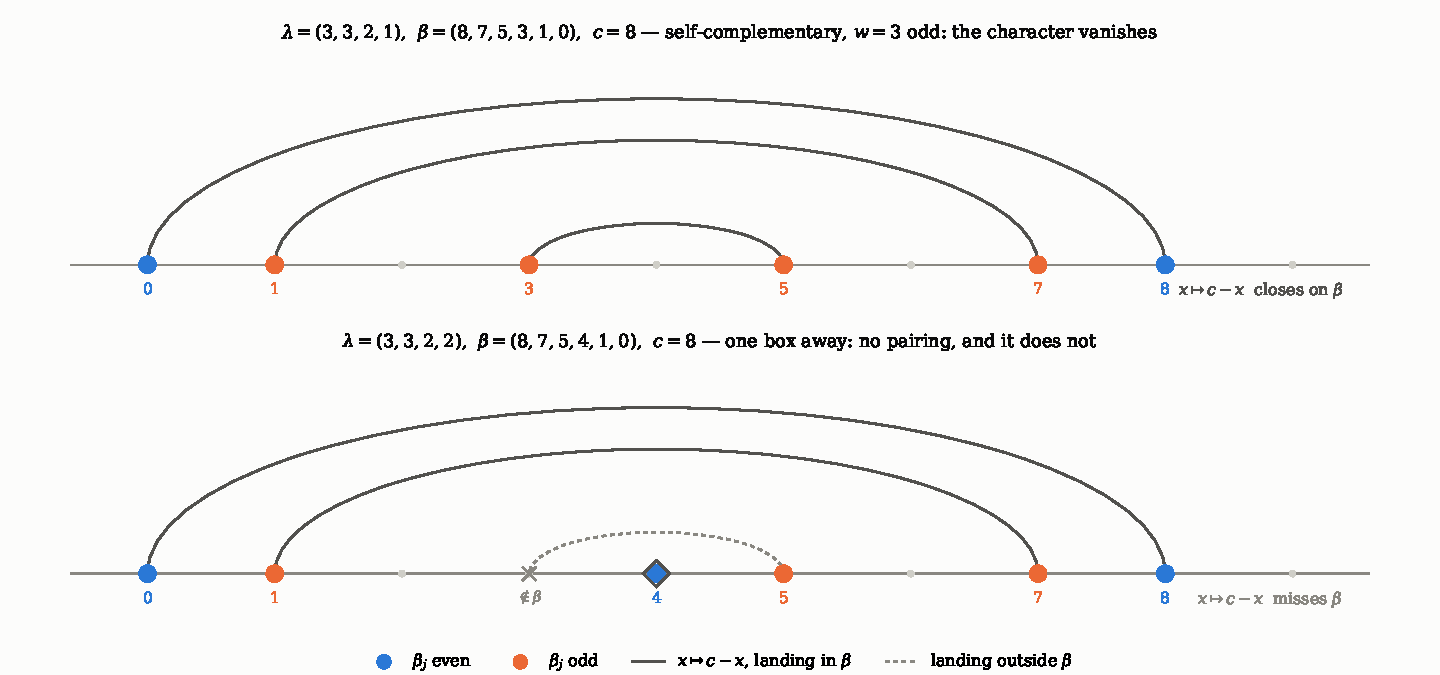
\includegraphics[width=\textwidth]{fig_involution.pdf}
\caption{Why self-complementarity kills the character. Expanding along the two frozen rows leaves
terms indexed by pairs $(e,o)$ with $e\in E$, $o\in O$, and the reflection $x\mapsto c-x$ acts on
them. Above, a self-complementary shape of odd width: every arc lands in $\beta$ and joins entries of
equal parity, because $c$ is even. Below, the same shape with one box moved: the arc $5\mapsto3$
leaves $\beta$, so there is no pairing and nothing cancels. The diamond marks the fixed point of the
reflection, which cannot occur inside an opposite-parity pair --- which is why the involution is
free.}
\label{fig:involution}
\end{figure}

\begin{proof}[Proof of Theorem \ref{thm:r1}]
Put $c_\ast=z+\bar z$ and let $S_n$ be defined by $S_0=0$, $S_1=1$,
$S_{n+1}=c_\ast S_n-S_{n-1}$, so $\deg_{c_\ast}S_n=n-1$ and $S_{-n}=-S_n$; the value $S_{-1}=-1$ is
used whenever $\beta_N=0$. Since $\Phi_A=(x^2-1)(x^2-c_\ast x+1)$, a polynomial $P$ supported on
$\beta$ is divisible by $\Phi_A$ exactly when $P(1)=P(-1)=0$ and $P\equiv0$ modulo $x^2-c_\ast x+1$.
Splitting $P(\pm1)$ by parity and reducing $x^n\equiv S_nx-S_{n-1}$, admissibility becomes the
singularity of the $4\times4$ matrix with rows $[\beta_j\ \mathrm{even}]$,
$[\beta_j\ \mathrm{odd}]$, $S_{\beta_j}$, $S_{\beta_j-1}$. Expanding along the two parity rows and
using d'Ocagne's identity \cite{Doc} for this recurrence,
\begin{equation}\label{eq:docagne}
S_bS_{b'-1}-S_{b'}S_{b-1}=-S_{b-b'},
\end{equation}
each $2\times2$ block collapses to a \emph{single} $S$, indexed by the difference of the two
surviving $\beta$'s. Distinct $S_n$ have distinct degrees in $c_\ast$ and are therefore linearly
independent, so the signed sum vanishes only by exact pairing of equal indices with opposite signs.
The case analysis is finite: $|E|\in\{0,4\}$ is branch (a); $|E|\in\{1,3\}$ leaves three terms whose
indices are the three pairwise differences of a $3$-set and hence always distinct, so no pairing
exists and the value is nonzero; and for $|E|=2$ there are four terms and three perfect matchings,
and one checks the six parity patterns directly. For $E=\{\beta_1,\beta_4\}$ and for
$E=\{\beta_2,\beta_3\}$ exactly one of the three matchings is available and it imposes the single
condition $\beta_1+\beta_4=\beta_2+\beta_3$, which is branch (b); for the four remaining patterns
every one of the three matchings forces two distinct entries of $\beta$ to coincide, so none is
available and the value is nonzero.
\end{proof}

Identity \eqref{eq:docagne} is classical. The collapse it produces is an accident of rank one: two
letters admit a single gap, so $s_{(m,n)}(z,\bar z)=S_{m-n+1}$ depends on that gap alone. There is no
rank-$r$ analogue. One would be a closed form for $s_\mu$ at a reciprocal alphabet for \emph{every}
$\mu$; \cite{CK09} supply that for rectangular shapes and \cite{AB19} for self-complementary ones,
and nobody in general.

For general $r$ we use associates, in Littlewood's sense \cite{Lit50}. On the $\det=-1$ coset $[\nu^{*}]=[\nu]\otimes\det$ gives
$\Psi_r=\sum_\nu\big(m_\nu-m_{\nu^{*}}\big)\chi_{[\nu]}$, so $\Psi_r=0$ if and only if
$m_\nu(\lambda)=m_{\nu^{*}}(\lambda)$ for every $\nu$; equivalently, $V_\lambda|_{O(N)}$ is
$\det$-invariant. A witness is therefore a single $\nu$ with $m_\nu\ne m_{\nu^{*}}$, and it can be
constructed.

Karmakar's \cite[Theorem 4.1]{Kar24} determines the value at the endpoint $z_i=1$, which is an element
of order two: case (A) is branch (a), case (B) is a nonzero dimension, and case (C) leaves an
alternating sum of products of dimensions with no vanishing criterion attached. Branch (b) lives in
that case (C), so the theorem below is not a consequence of it. Nor does case (B) help more as $r$
grows: at $k=1$ it asks that $N-1$ of the $N$ beta numbers share a parity, and the smallest shape
doing so is the staircase $(2r-1,2r-2,\dots,1)$, of size $r(2r-1)$, so on a fixed range of
$|\lambda|$ his nonvanishing case is visible only for small $r$ --- his result is sharpest exactly
where ours is easiest. What connects the endpoint to the
curve at all is rigidity, and rigidity is a statement about our object rather than about the order-two
element: over the ranges of \S\ref{sec:verif} it holds on $\ell(\lambda)\le N/2$ without exception
and fails outside, which is Remark \ref{rem:rankone}.

\begin{proof}[Proof of Theorem \ref{thm:stable}]
Branch (a) cannot occur: with $\ell(\lambda)\le N/2$ at least two trailing parts vanish, so $\beta$
contains two consecutive integers. In Littlewood's range
$m_\nu(\lambda)=\sum_{\beta'\ \mathrm{even}}c^{\lambda}_{\nu\beta'}$, and the term $\beta'=\emptyset$
gives $m_\mu\ge1$ for every $\mu\subseteq\lambda$. Take $\mu$ as follows. If
$\ell(\lambda)<N/2$, take $\mu=\lambda$: then $\ell(\lambda^{*})=N-\ell(\lambda)>\ell(\lambda)$, so
$\lambda^{*}\not\subseteq\lambda$ and $m_{\lambda^{*}}=0\ne m_\lambda$. If $\ell(\lambda)=N/2$ and
$\lambda_{N/2}$ is even, take $\mu=(\lambda_1,\dots,\lambda_{N/2-1})$; then
$\beta'=(\lambda_{N/2})$ is even, $\lambda/\mu$ is a horizontal strip and $m_\mu\ge1$ while
$\ell(\mu)<N/2$, so the previous computation applies to $\mu$. If $\ell(\lambda)=N/2$ and $\lambda$
is not a rectangle, let $j\le N/2-1$ be largest with $\lambda_j>\lambda_{j+1}$ and remove both the
last row and one box from row $j$; then $\beta'=(\lambda_{N/2}+1)$ is even and
$\lambda_j\ge\lambda_{N/2}+1$ keeps $\lambda/\mu$ a horizontal strip. In the remaining case
$\lambda=(k^{\,N/2})$ neither construction is available, and $k$ odd is branch (b) while $k$ even
falls to the second construction.
\end{proof}

\subsection{Outside Littlewood's range}\label{sec:unstable}

For $\ell(\lambda)>N/2$ the restriction rule acquires non-standard labels, and the modification rules
that reduce them are King's \cite{King71}; Koike and Terada \cite{KT87} record that the
type-$D$ specialization sends a universal character to $0$ or to $\pm$ one other, and Fauser, Jarvis,
King and Wybourne observe that beyond the two classical cases \emph{``the general theory, having
infinitely many cases, needs a not yet available formalism''} \cite[\S4]{FJKW05}. Extensions of Littlewood's rule to all parameters do exist for the two classical
cases --- Newell's modification rules \cite{New51}, Sundaram \cite{Sun90} in the symplectic case,
Gavarini's Brauer-algebra proof \cite{Gav99}, and Enright and Willenbring \cite{EW04}, whose Theorem 4
gives the multiplicity as an alternating sum over the Weyl group which in favourable cases collapses
to a difference of two Littlewood coefficients \cite[\S7.11]{EW04}. The route taken here is the dual
one: keep the coefficients universal, which they are in every range, and move the whole
range-dependence into the values, where one lemma disposes of it. On this alphabet no formalism for
the labels is needed at all, and the reason is that the values are not type-$D$ values.

Adding a letter $c$ to an alphabet acts on the ring of symmetric functions by $p_k\mapsto p_k+c^k$;
write $\iota_c$ for that homomorphism. From the generating function of the complete homogeneous
symmetric functions, $h_m(W,c)-c\,h_{m-1}(W,c)=h_m(W)$ for every $m$.

\begin{lemma}[the alphabet is symplectic]\label{lem:AtoSp}
$\iota_{-1}\iota_{1}\,o_\nu=sp_\nu$ for every partition $\nu$, as an identity between Koike--Terada
\emph{universal} characters in $\Lambda$. In particular, for the alphabet
\eqref{eq:psir},
\begin{equation}\label{eq:AtoSp}
o_\nu(A)\;=\;sp_\nu(z_1,\dots,z_r)
\end{equation}
with no hypothesis on $\ell(\nu)$ and with no sign. For $\ell(\nu)>r$ the right-hand side is
that universal character specialized at $r$ variables, not an irreducible $Sp(2r)$ character; it is
the modification rules below that fold it onto one.
\end{lemma}

\begin{proof}
Both steps are Ayyer and Kumari's, and both are the same manipulation: the recurrence turns the
column operations $C_j\to C_j-c\,C_{j-1}$, applied for $j=n,\dots,2$ in that order, into a change of
character type, and operations of that shape leave a determinant unchanged. At $c=1$ they carry the
defining determinant of $o_\nu$ evaluated at $(W,1)$ to that of the odd orthogonal universal
character $so_\nu$ over $W$, which is Koike and Terada's dictionary in the form
$so_\nu(X)=o_\nu(X,\bar X,1,0,0,\dots)$ \cite[(2.13)]{AK25}. At $c=-1$, where the recurrence is
\cite[Proposition 2.1]{AK25} and the operations read $C_j\to C_j+C_{j-1}$, they carry $so_\nu$ to
$sp_\nu$, which is \cite[Lemma 3.2]{AK25}. Composing gives the first statement, and evaluating it on
the reciprocal alphabet $(z_1,\dots,z_r)$ gives \eqref{eq:AtoSp}.
\end{proof}

\noindent Since $\nu'_1=\ell(\nu)$, the trichotomy on $\nu'_1$ against $N/2=r+1$ is a trichotomy on
the length of $\nu$ against the rank of $Sp(2r)$, and the three facts we need are then the classical
symplectic modification rules --- one of the two cases \cite{FJKW05} exempts --- read through
\eqref{eq:AtoSp}: $o_\nu(A)=0$ when $\ell(\nu)=r+1$, the vanishing of a symplectic character one row
past its rank; $o_\nu(A)=\pm o_{\nu^{*}}(A)$ when $\ell(\nu)>r+1$, King's rule folding the label back
onto a dominant one; and the same for non-standard $\nu$, which by Lemma \ref{lem:nonstd} are exactly
the tall ones. The expansion $s_\lambda=\sum_\nu c_\nu o_\nu$, with
$c_\nu=\sum_{\beta'\ \mathrm{even}}c^{\lambda}_{\nu\beta'}$, is an identity of symmetric functions and
holds in every range; specializing it at \eqref{eq:psir} therefore lands every term on
$\{o_\mu(A):\ell(\mu)\le r\}$, which by \eqref{eq:AtoSp} is the set of irreducible characters of
$Sp(2r)$ and so is linearly independent. Figure \ref{fig:reduction} sorts the labels into the four
classes this paragraph describes and computes $o_\nu(A)$ on each, so that the reduction can be seen
to land where it is claimed to. Hence

\begin{figure}[!ht]
\centering
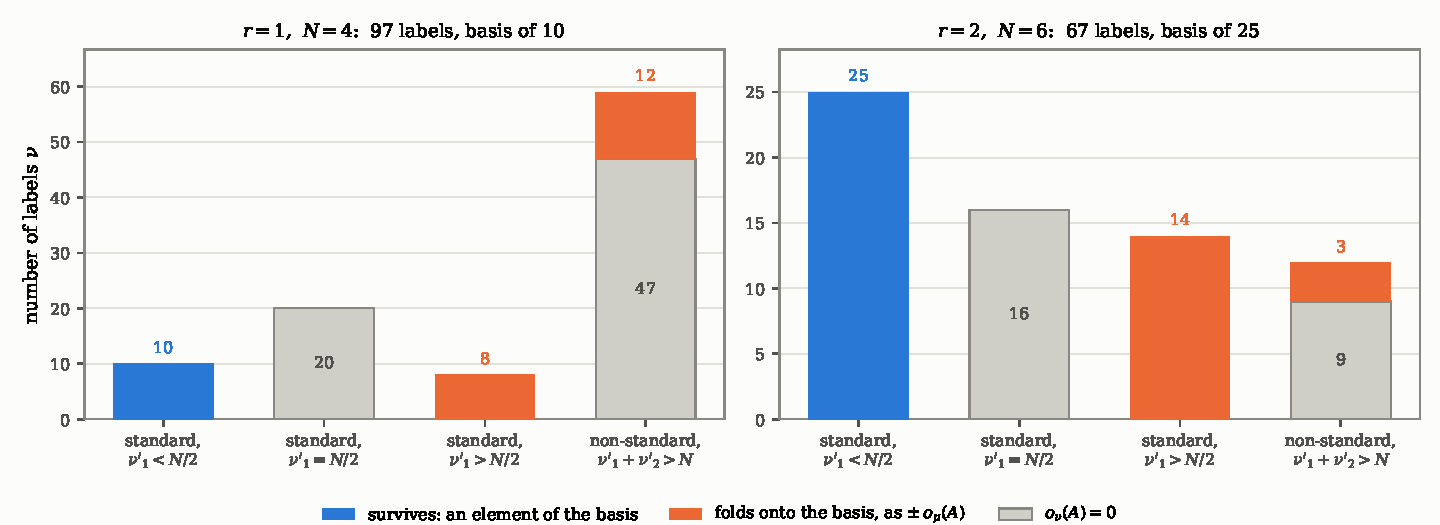
\includegraphics[width=\textwidth]{fig_reduction.pdf}
\caption{The reduction of Lemma \ref{lem:AtoSp}, drawn. Each label $\nu$
occurring in $s_\lambda=\sum_\nu c_\nu o_\nu$ is placed in one of four classes and its value
$o_\nu(A)$ computed. Self-associate labels vanish, every one of them; labels standard with
$\nu'_1>N/2$ fold onto the basis as $\pm o_{\mu}(A)$; non-standard labels either vanish or fold onto
a single basis element with coefficient $\pm1$. By \eqref{eq:AtoSp} these three are the symplectic
modification rules in disguise, the classes being cut by $\ell(\nu)$ against the rank $r$; the figure
was computed before that was noticed, and is left as drawn. Everything lands on the independent
basis $\{o_\mu(A):\ell(\mu)\le r\}$, which is what turns the vanishing into the finite condition
\eqref{eq:Cmu}. The bar heights are label counts over the range each panel was computed on, which is
smaller than the range of the corresponding row of \S\ref{sec:verif}; the classification, not the
count, is what the picture is about.}
\label{fig:reduction}
\end{figure}
\begin{equation}\label{eq:Cmu}
\Psi_r(\lambda)=\sum_{\ell(\mu)\le r}C_\mu(\lambda)\,o_\mu(A),
\qquad
\Psi_r(\lambda)=0\iff C_\mu(\lambda)=0\ \text{for all }\mu,
\end{equation}
where $C_\mu=c_\mu\pm c_{\mu^{*}}+\sum\pm c_\nu$ over the non-standard $\nu$ reducing to $\mu$. The
reduction is carried out in two steps rather than one: most non-standard labels pair with an associate
inside the range, while $21$ of them --- $18$ at $r=1$ and $3$ at $r=2$ --- have no associate in range
and are reduced separately, each landing in the span of the standard values with integer coefficients.

We had computed the three facts before locating them, and record the computation because it is what
the figure below draws: \texttt{sec8\_derivation.sage} checks \eqref{eq:AtoSp} directly for all
$|\nu|\le8$, confirms that the labels of length $r+1$ vanish and that longer ones fold onto the basis
with a sign, and verifies the independence as a rank computation, at $r=1,2,3$. A control that had to
fire: $\iota_1 o_\nu$ and $\iota_{-1}o_\nu$ each agree with $sp_\nu$ only for $\nu=\varnothing$, so
both letters are needed and \eqref{eq:AtoSp} is a statement about the reciprocal pair, not about
either letter alone. \texttt{sec8\_formulas.sage} checks the proof rather than the statement --- the
recurrence at four values of $c$, the two defining determinants against an independent
implementation, and the column operations entry by entry. That last check earned its keep: an earlier
draft of the proof wrote $C_j\to C_j+C_{j-1}$ at $c=1$, the sign \cite[Lemma 3.2]{AK25} uses for its
own step at $c=-1$.

The non-standard labels, which are the whole obstruction here, cannot be small:

\begin{lemma}[non-standard labels are large]\label{lem:nonstd}
Every non-standard $\nu$ occurring in the expansion satisfies $|\nu|\ge N+1=2r+3$. Consequently, if
$|\lambda|\le2r+2$ then no non-standard label is contained in $\lambda$, the last sum in $C_\mu$ is
empty, and $C_\mu(\lambda)=c_\mu(\lambda)\pm c_{\mu^{*}}(\lambda)$ --- with no hypothesis on
$\ell(\lambda)$, hence also outside Littlewood's range.
\end{lemma}

\begin{proof}
Since $c^{\lambda}_{\nu\beta'}=0$ unless $\nu\subseteq\lambda$, only labels with
$\ell(\nu)\le\ell(\lambda)\le N$ occur. Non-standard means $\nu'_1+\nu'_2>N$. Were $\nu$ a single
column we would have $\nu'_2=0$ and hence $\nu'_1=\ell(\nu)>N$, which is excluded; so $\nu'_2\ge1$ and
$|\nu|\ge\nu'_1+\nu'_2>N=2r+2$. A non-standard $\nu$ can therefore contribute only when
$|\lambda|\ge|\nu|\ge2r+3$.
\end{proof}

\noindent Since $\ell(\lambda)>N/2$ forces $|\lambda|\ge r+2$, Lemma \ref{lem:nonstd} settles the
band $r+2\le|\lambda|\le2r+2$ of the unstable range outright: there Littlewood's rule applies
verbatim and the converse follows by the argument of Theorem \ref{thm:stable}. What is left open is
$|\lambda|>2r+2$.


Two exact facts bound the competitors. First $\ell(\mu^{*})=N-\ell(\mu)$, so $\ell(\mu)\le
N-1-\ell(\lambda)$ forces $\mu^{*}\not\subseteq\lambda$ and $c_{\mu^{*}}=0$. Second, a non-standard
$\nu$ has $\nu'_1+\nu'_2>N$ with $\nu'_2\le\nu'_1$, hence $2\ell(\nu)>N$ and $\ell(\nu)\ge r+2$; in
particular no non-standard label fits inside $\lambda$ in Littlewood's range. Call $\mu$
\emph{isolating} for $\lambda$ if exactly one of the labels feeding $C_\mu$ is contained in
$\lambda$; then $C_\mu=\pm c_\nu\ne0$ and $\Psi_r(\lambda)\ne0$. What remains open is one existence
statement.

\begin{proposition}[the isolating witness does not always exist]\label{conj:iso}
At $r=2$ the shape $\lambda=(5,5,2,1)$ has $\Psi_2(\lambda)\ne0$ and is of neither type {\rm(a)} nor
type {\rm(b)}, and no $\mu$ is isolating for it: every $\mu$ whose $C_\mu$ has a nonzero contributor
inside $\lambda$ has exactly two, namely $\mu$ and its associate $\mu^{*}$.
\end{proposition}

We had proposed the isolating witness as the route to Conjecture \ref{conj:crit}, and it does not
reach. The reason is legible in the isolation lemma: it needs $\ell(\mu)\le N-1-\ell(\lambda)$, which
at $\ell(\lambda)=4$ and $N=6$ leaves only one-row $\mu$, and a shape as wide as $(5,5,2,1)$ contains
every associate. Over $r=2$ and $|\lambda|\le14$ there are eleven such shapes, and none at all below
$|\lambda|=13$, which is why the certificate looks sound on small ranges. Conjecture \ref{conj:crit}
itself is untouched --- it asserts that the $C_\mu$ vanish, not that a certificate exists, and it
holds over every shape in the ranges of \S\ref{sec:verif} --- but it is left without a route.

The mechanism does reach a great deal: at $r=2$ and $|\lambda|\le14$, $227$ of the $238$ non-vanishing
unstable shapes carry a proved isolating witness. It also reaches further than fact (ii) allows on
its own --- the true minimum of $\ell(\nu)$ over non-standard $\nu$ with $o_\nu(A)\ne0$ is $5$ there,
against the $r+2=4$ the bound gives. What defeats it is width rather than height: the basis in
\eqref{eq:Cmu} grows with $r$ and the competing labels are constrained to be tall, so we had read
isolation as getting easier with $r$, and along the height axis it does; the residue lives where
$\lambda$ is wide enough to swallow the associates. That reading predicts where the residue is
\emph{not}: at $r=3$ the isolation lemma allows $\ell(\mu)\le7-\ell(\lambda)$, so a shape must be
wider than at $r=2$ before it can swallow every associate, and the same sizes should come out clean.
They do --- over $r=3$ and $|\lambda|\le13$ all $149$ non-vanishing unstable shapes carry a proved
witness and the residue is empty --- which is a control on the explanation rather than a step toward
the conjecture. At $r=1$ the question does not arise, since that case is settled independently by
Theorem \ref{thm:r1}.

The tool one reaches for first does not fit. Saturation, in the honeycomb form of Knutson and Tao
\cite{KT99}, decides when a single Littlewood--Richardson coefficient is positive, and every
competitor feeding $C_\mu$ is positive as soon as its label sits inside $\lambda$. What an isolating
$\mu$ asks for is not positivity but \emph{isolation}: that exactly one of them does. The positivity
is what makes the question hard rather than what answers it, and we know of no tool aimed at the
second question.

\begin{figure}[tb]
\centering
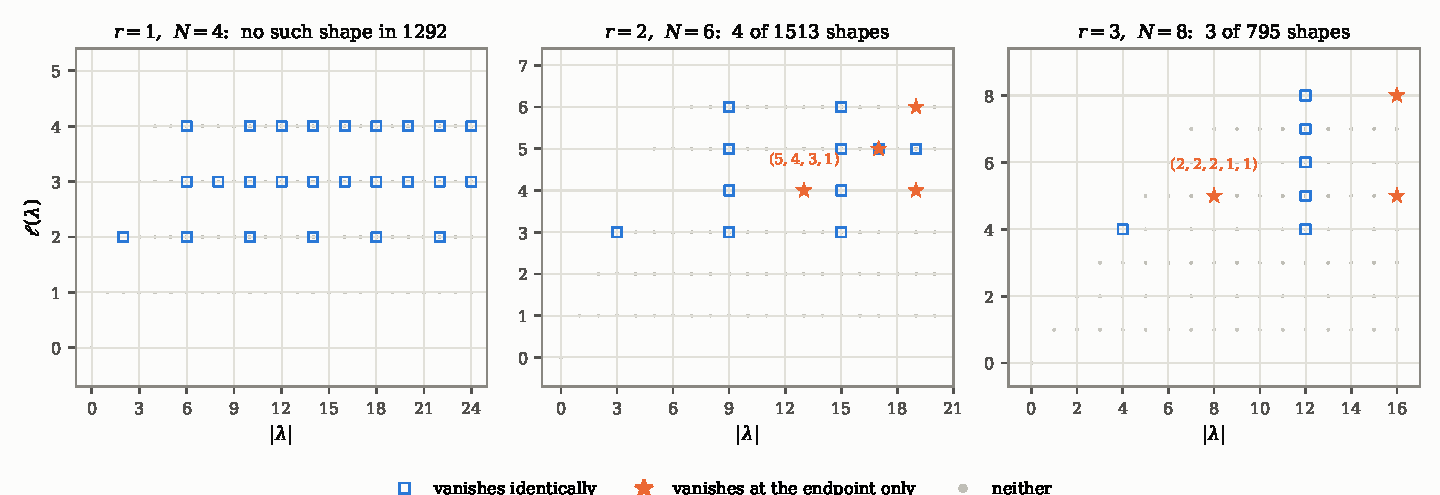
\includegraphics[width=\textwidth]{fig_phase.pdf}
\caption{Where one reciprocal pair stops being typical. Each partition with at most $N$ parts is a
point at $(|\lambda|,\ell(\lambda))$; the class drawn as a star is the one that vanishes at the
endpoint $z_i=1$ without vanishing identically, and it is the whole content of the picture; each
panel names its smallest member and Remark \ref{rem:rankone} lists the rest. The panels cover
$|\lambda|\le24$, $20$ and $16$ respectively. At $r=1$ the class is
empty over all $1292$ shapes in range, because the object there is $\pm$ a genuine character and its
value at the identity is a dimension. From $r=2$ on the object is properly virtual and the class is
not empty. See Remark \ref{rem:rankone}.}
\label{fig:phase}
\end{figure}

\begin{remark}[the rank-one accident, and where the two ranges part]\label{rem:rankone}
At $r=1$ the object is $\pm$ a genuine character, so its value at the identity is a dimension and
$\Psi_1(\lambda)\equiv0$ if and only if $\Psi_1(\lambda)|_{z=1}=0$. At $r\ge2$ the object is properly
virtual and that equivalence fails: $\lambda=(5,4,3,1)$ at $r=2$ has $\Psi_2(\lambda)\ne0$ and
$\Psi_2(\lambda)|_{z_1=z_2=1}=0$. Over the ranges of Figure \ref{fig:phase} the class of such shapes
is empty at $r=1$ across $1292$ partitions; at $r=2$ it consists of the four shapes $(5,4,3,1)$,
$(5,5,4,2,1)$, $(10,5,3,1)$ and $(6,5,4,2,1,1)$, and at $r=3$ of the three shapes $(2,2,2,1,1)$,
$(5,5,4,1,1)$ and $(3,3,3,2,2,1,1,1)$; it is thin, but it is not empty, and one counterexample is all
the equivalence can survive. The surviving implication, exact vanishing $\Rightarrow$ vanishing
at the endpoint, is what makes the endpoint a valid sieve and no more. This is why results computed
at elements of order two \cite{Kar24}, or at variables set to $1$ \cite{Eis07}, bear on the endpoint
and not on the curve, and why Theorem \ref{thm:zeros} is not a corollary of them for $r\ge2$.
\end{remark}

It is worth putting a number on what the endpoint sieve loses, since the qualitative statement is
easy to misread as a small correction. Over the ranges of Figure \ref{fig:phase} the test
$\Psi_r(\lambda)|_{z_i=1}=0$ flags $143$ shapes at $r=1$, $22$ at $r=2$ and $9$ at $r=3$; of those,
$0$, $4$ and $3$ respectively do not vanish identically. So the sieve is exact at one pair, and the
fraction of its verdicts that are spurious grows with the number of pairs --- $0\%$, $18\%$, $33\%$
over these ranges. An endpoint computation is a filter that never misses a genuine zero, and past one
pair it is nothing more than that. The rank-one case at $t=2$, where the sieve happens to be exact
because the object is a genuine character, was treated separately in \cite{Mar26}; the alphabet
\eqref{eq:object} arose there, in a Wilson-line computation on an orbifold, which is why $-1$ appears
as a letter rather than as a choice.

The reason the two ranges of $\ell(\lambda)$ behave so differently is worth separating from the
mechanism that proves it. Littlewood's rule is a statement about which labels $\nu$ can occur, and
$\ell(\lambda)\le N/2$ is exactly the condition under which the non-standard ones cannot fit inside
$\lambda$ at all. Lemma \ref{lem:nonstd} says that the obstruction is governed by $|\lambda|$ as well
as by $\ell(\lambda)$, so the honest picture is not two ranges but a region: the converse is proved
wherever either $\ell(\lambda)\le N/2$ or $|\lambda|\le2r+2$, and outside their union it is open ---
the isolating witness covers most of that region but provably not all of it, by Proposition
\ref{conj:iso}.

%======================================================================
\section{Verification}\label{sec:verif}

Every statement above was checked numerically, by two implementations along different code paths: one
in exact Laurent arithmetic, and one a from-scratch bialternant evaluation written from the
statements alone. The ranges and counts are collected here once.

\begin{center}\footnotesize\setlength{\tabcolsep}{4.2pt}
\begin{tabular}{llrl}
\toprule
statement & range & result & status\\
\midrule
Theorem \ref{thm:main}, sign included & $t\le7$, $|\lambda|\le14,\dots,10$ &
$959$ exact, $476$ zeros, $0$ fail & \stproved\\
Lemma \ref{lem:L1} & $t\le6$ & $454$ nonzero minors & \stproved\\
Lemma \ref{lem:L4} & $t\le7$ & $724/724$ & \stproved\\
Proposition \ref{prop:quotient} & $t\le7$, $|\lambda|\le19$ & $2970/2970$ & \stproved\\
Proposition \ref{rem:lattice} (the concentric locus) & $t\le9$, $|\lambda|\le16$ & $1331/1331$;
$0$ at odd $t$, $43$ at even & \stproved\\
Proposition \ref{rem:sign} (short form of the sign) & $t\le8$, $|\lambda|\le14$ & $1496/1496$;
proof steps $0$ fail & \stproved\\
Proposition \ref{prop:fibrelattice} (the lattice) & $t\le5$, $|\lambda|\le14,12,10,10$ &
$84$, $35$, $20$, $14$ fibres, both ways & \stproved\\
Corollary \ref{cor:fibregf} (the generating function) & same range &
$153/153$; wrong denominator $101$ & \stproved\\
Remark \ref{rem:signsees} (the sign sees the $m_i$) & $t\le4$ &
$107/107$, $43/62$, $26/36$ & \stverif\\
Lemma \ref{lem:single} & $t\le7$, $|\lambda|\le16$ & $2113/2113$ & \stproved\\
Theorem \ref{thm:extra} & $t\le12$, $\lambda_1\le33$ & $119+21$, no others & \stproved\\
Proposition \ref{prop:rect} & $t=2$, $r\le4$, $c\le60$ & $240/240$ & \stproved\\
Corollary \ref{cor:enum} against direct enumeration & $t\le5$ & $14/14$; boxes $16/16$ &
\stproved\\
Proposition \ref{rem:involution} (the runs alternate) & $t=2$, $|\lambda|\le14$, $\le4$ rows &
$4823$ minors; $217$ pairs, $0$ fail & \stproved\\
(D3), (D4) of \S\ref{sec:sharp} & $t\le6$, $|\lambda|\le10$ &
$600$ / $383$ / $200$ of $600$ & \stverif\\
\midrule
\rowcolor{hband} Theorem \ref{thm:zeros}, both directions & $r\le3$, $|\lambda|\le28,26,22$ &
$9961$ shapes, $318$ zeros, $0$ fail & \stverif\\
\rowcolor{hband} \quad branch (a), Thm.~\ref{thm:zeros} & $r\le3$, $|\lambda|\le15$ &
$16/16$ & \stproved\\
\rowcolor{hband} \quad branch (b), Thm.~\ref{thm:zeros} & $r\le3$ & $24/24$ & \stproved\\
\rowcolor{hband} \quad even-width control for (b) & $r\le3$ & $56/56$ nonzero & \stproved\\
\rowcolor{hband} \quad converse at $r=1$, Thm.~\ref{thm:r1} & $\beta_1\le25$ &
$14950$ beta sets, $0$ fail & \stproved\\
\rowcolor{hband} \quad converse, $\ell(\lambda)\le N/2$, Thm.~\ref{thm:stable} & $r\le3$ &
$372/372$ witnesses & \stproved\\
\rowcolor{hband} \quad the isolating witness, Prop.~\ref{conj:iso} & $r=2$, $|\lambda|\le14$ &
$227$ witnesses, $11$ residue & \stproved\\
\rowcolor{hband} \quad the same at $r=3$ & $r=3$, $|\lambda|\le13$ &
$149$ witnesses, $0$ residue & \stproved\\
\midrule
Identity \eqref{eq:compl} & $r\le2$ & $474/474$ & \stproved\\
Identity \eqref{eq:docagne}, and $\deg_{c_\ast}S_n=n-1$ & $b\le31$ & $496/496$; $39/39$ &
\stproved\\
Lemma \ref{lem:AtoSp}, the \S\ref{sec:unstable} reduction & $r\le3$, $|\nu|\le8$ &
identity $0$ fail; folds $0$ fail & \stproved\\
\quad the reduction carried out & $r\le2$ & $236$ labels, $0$ unresolved & \stproved\\
\eqref{eq:Cmu} against the exact object & $r\le2$, both ranges & $184$ shapes, $0$ fail &
\stverif\\
\bottomrule
\end{tabular}
\end{center}

\noindent The shaded block is Theorem \ref{thm:zeros} read from the top down: the two sufficient
branches are proved for every $r$, the converse is proved for one pair and, for every $r$, inside
Littlewood's range, and one line remains --- the converse for $r\ge2$ outside that range and beyond
the band $|\lambda|\le2r+2$ that Lemma \ref{lem:nonstd} settles, which is Conjecture
\ref{conj:crit}. That single \stverif\ line is why the first row of the block is not
labelled \stproved. The row below it records what the certificate we proposed for that line does and
does not do, and it is labelled \stproved\ because Proposition \ref{conj:iso} is a counterexample and
counterexamples are proofs. The rows below the block are the identities and the reduction the section rests
on. In the column, \stproved\ means a proof is given here or cited, and \stverif\ means the
statement is checked exhaustively over the stated range and not proved.

\noindent The (D3), (D4) row is the one that matters most in the first group: the identity holds in
all $600$ cases for \eqref{eq:object} and fails in $217$ and $400$ of them for the two deformed
alphabets, so the test is capable of failing. In the second group the even-width control plays the
same role for Theorem \ref{thm:zeros}: $56$ self-complementary shapes of even width, none of which
vanishes, so the parity hypothesis is doing work rather than decorating. A separate audit rebuilds
all of the second group from the definitions in a single pass, independently of the scripts that
produced them: $3414$ checks, $0$ failures. A second one takes the \emph{displayed formulas} rather
than the counts --- Theorem \ref{thm:LR}, the interval reading \eqref{eq:intervals}, Lemmas
\ref{lem:L2} and \ref{lem:L5}, the splitting \eqref{eq:threestep}, the complementation
\eqref{eq:compl}, d'Ocagne \eqref{eq:docagne} and the scalar caveat \eqref{eq:scalar} --- and
evaluates both sides at numeric points from the definitions, using neither the closed forms of this
paper nor the scripts behind the table: $3297$ evaluations over nine displayed formulas, $0$ failures. The scripts are ancillary to this paper, and so is the
saved output of each one, so every count in the table above can be located in an archived run rather
than taken on trust.

%======================================================================
\section{Open problems}\label{sec:open}

\begin{problem}[the other classical types]\label{prob:types}
Everything above is type $A$. What do $sp_\lambda(\zt,z,\zb)$, $so_\lambda(\zt,z,\zb)$ and
$o_\lambda(\zt,z,\zb)$ do? The root-of-unity factorizations were carried from type $A$ to $B$, $C$,
$D$ by a uniform argument in \cite{AK22} and to the universal characters in \cite{Alb23}; the frozen
rows of the bialternant are the same in every type, so Lemma \ref{lem:L1} and the excess-two count
should survive verbatim, while the collapse, Lemmas \ref{lem:L4} and \ref{lem:L5}, would need
re-deriving once per type. The alphabet \eqref{eq:object} is already a torus element of $O(t+2)$, so
the other types are not the same function at a new point but new objects, and choosing the right ones
is a matter of taste inside a programme we did not build. We have measured, and report it as a
measurement only. Expanding the Koike--Terada universal characters in the Schur basis and evaluating
term by term with Theorem \ref{thm:main}, over $|\lambda|\le12$ for $t\le3$ and $|\lambda|\le10$ for $t=4,5$, the fraction of
$\ell(\lambda)\ge2$ shapes on which the value vanishes is markedly larger for $o_\lambda$ on the
non-identity component than on the identity one --- $83.8\%$ at $t=2$ against $41.8\%$ at $t=3$, and
$58.8\%$ at $t=4$ against $42.1\%$ at $t=5$ --- with $sp_\lambda$ in between and the Schur case
lowest. The effect is real and it tracks the component, which is what one would expect of an
associate cancellation; but it is quantitative and we found no law covering the whole table. A first
attempt at one, that
$o_\lambda$ vanishes for all $\ell(\lambda)\ge2$ when $t$ is even, is false: it was read off a
sample and the systematic sweep refutes it.

The $t=2$ column of that comparison is the one case which does have a law, and it is Lemma
\ref{lem:AtoSp}: there the alphabet is \eqref{eq:psir} at $r=1$, so $o_\nu$ equals $sp_\nu(z)$, a
\emph{rank-one} symplectic character. That vanishes identically for $\ell(\nu)=2$ --- all $36$ such
shapes in range, with no exception --- and folds for $\ell(\nu)>2$, which is why the $t=2$ figure is
the outlier. What remains without a law is odd $t$, where the alphabet is not of the form
\eqref{eq:psir} and the lemma does not apply.

The $sp_\lambda$ column at $t=2$, on the other hand, has an answer, and it explains the asymmetry of
the table rather than adding a row to it. Adjoining the same two letters to a universal
\emph{symplectic} character does not collapse it. Over $|\nu|\le8$,
\begin{equation}\label{eq:spbranch}
sp_\nu(W,1,-1)\;=\;\sum_{\gamma\subseteq\nu}c_{\nu/\gamma}\;sp_\gamma(W),
\end{equation}
where the coefficient depends on $\nu$ and $\gamma$ only through the skew shape $\nu/\gamma$ ---
$247$ coefficients over $74$ distinct skew shapes, with no clash --- and takes only the values $0$
and $\pm1$, vanishing whenever $|\nu/\gamma|$ is odd. That is the shape a branching rule for
universal symplectic functions produces, and such rules are available \cite{JJLW24}. Read against it,
Lemma \ref{lem:AtoSp} says that for $o_\nu$ the corresponding coefficients are concentrated at
$\gamma=\nu$: the two letters collapse the orthogonal character to a single symplectic one, and leave
the symplectic character spread over the whole interval below $\nu$. The asymmetry of the measurement
is that, and not an artefact of the ranges. What we have not done is identify $c_{\nu/\gamma}$, which
\eqref{eq:spbranch} makes a question about skew universal symplectic characters at $(1,-1)$ and
nothing more.

The third column resists the same route, and for a structural reason rather than an accidental one.
What answers the other two is that adjoining a letter is the ring map $p_k\mapsto p_k+c^k$, so
$\iota_{1}$ and $\iota_{-1}$ act on $\Lambda$ and compose. The identity that would bring $so$ into
the picture, $so_\nu(X)=o_\nu(X,\bar X,1,0,\dots)$ of \cite[(2.13)]{AK25}, relates the two on a
\emph{doubled} alphabet instead, and a doubling is not an adjunction: the $\iota$'s do not reach it.
So the $so$ column is not a gap of effort but of mechanism, and we leave it stated as such.
\end{problem}

\begin{problem}[a Verschiebung that sees a reciprocal pair]\label{prob:versch}
The operator $\varphi_t$ has nothing to say about a letter outside a $\zeta$-orbit, which is the
structural reason Theorem \ref{thm:main} is not a corollary of anything in that line, and the reason
our proof descends to the alternant. Is there an operator on universal characters, or a
factorization of $\varphi_t$ through a larger algebra, acting on alphabets of the form (union of
$\zeta$-orbits) $\cup$ (reciprocal pairs)? By \S\ref{sec:sharp} such an operator would decide (D1)
and (D2) at once. The discussion there suggests a quantitative form.

What makes the question well posed rather than vague is that each half already has a formalism, and
they are not the same one. The $\zeta$-orbits are the province of $\varphi_t$, in Albion's
formulation \cite{Alb23}. Alphabets closed under inversion are the province of the universal
symplectic and orthogonal functions, which have vertex operator realizations from which their
branching rules follow \cite{JJLW24}. Our alphabet is one of each, and Lemma \ref{lem:AtoSp} is the
one place where the two meet: there the $\zeta$-orbit is $\{1,-1\}$, small enough that adjoining it
is a pair of letter maps rather than an operator. We know of nothing that acts on both halves at
once, and the question is whether the two formalisms compose.
\end{problem}

\begin{proposition}[the rank is the wrong invariant]\label{conj:rank}
Let $A=\zt\cup B$ with $B$ closed under inversion and disjoint from $\zt$, and let $\rho(B)$ be the
rank of the subgroup of $\CC^{\times}$ generated by $B$. Then $\rho(B)=1$ does not imply that
$s_\lambda(A)$ is a product of characters. At $t=2$ and $B=\{z,z^{-1},z^{2},z^{-2}\}$, which has
$\rho(B)=1$, the value at $\lambda=(2)$ has a root off the unit circle, and so has no such
factorization; the same happens for $B=\{z,z^{-1},z^{3},z^{-3}\}$.
\end{proposition}

\begin{proof}
A product of characters $\chi_k(z)=(z^{k+1}-z^{-k-1})/(z-z^{-1})$ has all of its roots on the unit
circle. For $B=\{z,z^{-1},z^{2},z^{-2}\}$ and $\lambda=(2)$ the value is
$z^{-4}+z^{-3}+z^{-2}+z^{-1}+3+z+z^{2}+z^{3}+z^{4}$, whose roots miss the circle by $0.32$; over
$|\lambda|\le8$ this happens for $17$ of the $62$ nonvanishing shapes, and for
$B=\{z,z^{-1},z^{3},z^{-3}\}$ for $18$. On the same range $B=\{z,z^{-1}\}$ has every root on the
circle without exception, as Theorem \ref{thm:main} requires.
\end{proof}

What the rank does not see is how many free directions $B$ has. A single reciprocal pair is one
direction; $\{z,z^{-1},z^{2},z^{-2}\}$ generates a group of rank one and is two, and the two see each
other. So the invariant to conjecture on is not $\rho(B)$ but the number of independent letters,
and with that reading the statement becomes the one \S\ref{sec:sharp} already makes by other means:

\begin{conjecture}[one free direction]\label{conj:rank2}
$s_\lambda(\zt\cup B)$ is a product of characters for every $\lambda$ if and only if $B$ is a single
reciprocal pair.
\end{conjecture}

The evidence for it is Theorem \ref{thm:main} in one direction and (D1)--(D4) together with
Proposition \ref{conj:rank} in the other: enlarging $B$ destroys the product whether the enlargement
raises the rank or not. We have no proof and no proposed mechanism, and this is precisely the
statement a $\varphi_t$-style argument ought to produce.

One caveat, which the conjecture as stated does not cover. Inversion-closure of $B$ is sufficient in
the evidence above, but it is not necessary for a product. Write $w=-iy$. Then the second block of
the alphabet $\{1,-1,y,-y^{-1}\}$ is not closed under inversion, yet
\begin{equation}\label{eq:scalar}
s_\lambda\big(1,-1,y,-y^{-1}\big)\;=\;i^{\,|\lambda|}\,s_\lambda\big(-i,\,i,\,w,\,w^{-1}\big),
\end{equation}
and the alphabet on the right is. The honest hypothesis is therefore that $A$ be a scalar multiple of
an inversion-closed set. A coset $\zeta\zt$ is itself inversion-closed exactly when
$\zeta^{2}=\pm1$, which is where (D3) does and does not break.

\begin{problem}[the instrument for the second pair]\label{prob:instrument}
Section \ref{sec:zeros} reduces the vanishing at $r\ge2$ to a statement about the coefficients
$C_\mu$ of \eqref{eq:Cmu}, which are signed sums of Littlewood coefficients, and Conjecture
\ref{conj:crit} is what remains --- with no certificate for it, since the one we proposed fails by
Proposition \ref{conj:iso}. Lemma \ref{lem:AtoSp} settles the other half of the reduction --- what
the values $o_\nu(A)$ are --- and settles it symplectically: the two readings of the alphabet agree
because they are the same reading, the orbit Lie algebra of $D_{r+1}$ being $C_r$ rather than the
fixed subalgebra $B_r$. What it does not touch is the coefficients. Kumari and Stokke \cite{KS26}
have given Murnaghan--Nakayama rules for symplectic, orthogonal and orthosymplectic Schur functions;
by Lemma \ref{lem:AtoSp} the relevant one here is the symplectic \cite[Theorem 3.4]{KS26}, not the
even orthogonal \cite[Theorem 3.10]{KS26}. Does the recursion it provides compute $C_\mu$? Their rule
carries a third sum beyond the adding and removing of border strips, and it is the one they single out
as complicated; \cite[Corollary 3.5]{KS26} shows it drops out once $\mu_n+1\ge r$, so it is a
shallow-shape phenomenon. An earlier form of this problem asked whether that sum is what accounts for
the failure of Littlewood's rule outside its range; Lemma \ref{lem:AtoSp} answers that it is not,
since the failure is carried by the symplectic modification rules, which act on the labels and not
inside the recursion. The coefficients are what is left, and whether that recursion computes them is
what we have not attempted.
\end{problem}

\begin{problem}[the extra locus, in general]\label{prob:extralocus}
Does Theorem \ref{thm:extra} have an analogue for $sp$, $so$ and $o$? More generally, for which
specializations of the free variables does the criterion \eqref{eq:AK53} acquire extra solutions, and
can the extra locus always be read off the kernel of the specialization acting on the span of the
universal characters, as Remark \ref{rem:why} suggests? If each type acquires a family indexed by an
order-two element of the residue lattice, the principle is real.

The question needs the free part pinned down, and for a computed reason: the extra family is a
phenomenon of the \emph{minimal} alphabet. Adjoin a second reciprocal pair and it is gone --- over
$t=3,4,5,6$ and $|\lambda|\le14$ the locus is then exactly the $t$-cores, for type $s$ no less than
for $sp$ and $o$, while at one pair type $s$ has the two extras of Theorem \ref{thm:extra} at $t=4$
and one at $t=6$. (We test the second pair at $z_2=z_1^{2}$, a specialization, which can only create
coincidences and not remove them, so a count of zero there is a count of zero.) An analogue for
another type must therefore be sought at \emph{that type's} minimal free part, one letter of each
kind; comparing types across free parts of different sizes measures the free part instead, which is
what our first attempt did.

The kernel is the right thing to look at, but its \emph{presence} does not settle the locus; its
size does. Two free parts of the same size can both collapse the independence and behave quite
differently. On the reciprocal locus $s_\mu(z,\zb)=\chi_{\mu_1-\mu_2}(z)$ retains one grading, and
the extra locus is the single family of Theorem \ref{thm:extra}. Replace the pair by the
$\zeta_2$-orbit $(z,-z)$, where $s_\mu(z,-z)=z^{|\mu|}s_\mu(1,-1)$ retains only $|\mu|$ and a sign,
and over $\ell(\lambda)\le2$ the criterion acquires $28$ further solutions at $t=2$ and $186$ at
$t=8$, in no family we can name. The control is the free pair $(z,w)$, which has no kernel and
returns the $t$-cores and nothing else at every $t\le8$ --- that is \eqref{eq:AK53} itself, so the
control is their theorem rather than a measurement of ours. So the
reciprocal pair is the collapsing specialization of \emph{smallest} kernel, and that, rather than
the mere existence of a kernel, is what makes its extra locus one family.
\end{problem}

\begin{problem}[the fibres, refined by the sign]\label{prob:fibres}
Corollary \ref{cor:fibregf} describes the fibre of the interval triple, and only that. The invariant
is $I_t=(d_1,d_2,d_3,\varepsilon_\lambda)$, and the sign cuts each branch further. Its cut is not
bookkeeping, and it is not idle: by Remark \ref{rem:signsees} the sign sees the $t-2$ directions the
triple does not, from $t=3$ on --- constant in $(m_i)$ at fixed $v$ in all $107$ slots at $t=2$, but
in only $43$ of $62$ at $t=3$ and $26$ of $36$ at $t=4$. What is the restriction of
$\varepsilon_\lambda$ to a branch? The obstruction to reading it off \eqref{eq:fibrelattice} is
visible in \eqref{eq:sign}: $\inv(b_S)$ is a statistic of the whole beta-word, and the lattice
coordinates split that word into two distinguished classes and $t-2$ free letters, so a rule would
have to reassemble what the bijection separates.

Two smaller gaps go with it. The same description for the size-three profile should be the same
bookkeeping with one class of three in place of two of two; we have not written it. The degenerate
profile is a different question, since there the fibre is the whole vanishing locus of $\Phi_t$,
which Corollary \ref{cor:zero} and Proposition \ref{rem:lattice} describe by other means.
\end{problem}

\begin{problem}[a sieving phenomenon that keeps a parameter]\label{prob:sieving}
At $t=2$ Corollary \ref{cor:enum} is a signed count of $\mathrm{SSYT}(\lambda,4)$, and a signed count
of order two is what Stembridge's $q=-1$ phenomenon \cite{Ste94} computes: on a set carrying an
involution, the value at $-1$ counts the fixed points. That is the case $\#C=2$ of the cyclic sieving
phenomenon of Reiner, Stanton and White \cite{RSW04}, whose Theorem 4.3 evaluates the principal
specialization $s_\lambda(1,q,\dots,q^{k-1})$ at a primitive $d$-th root of unity in terms of the
$d$-core and the $d$-quotient of $\lambda$ --- the two invariants that carry Theorem \ref{thm:main}
as well --- and which Lee and Oh \cite{LO22} have since extended to skew shapes. Every evaluation in
that line is at a \emph{number}, as a sieving statement requires: the alphabet there is the geometric
progression $1,q,\dots,q^{k-1}$ specialized at a root of unity, not a plain orbit, and nothing is
left free. Ours is not of that kind --- the reciprocal pair keeps $z$, and \eqref{eq:main} is a
product formula in it. Is there a cyclic action on $\mathrm{SSYT}(\lambda,t+2)$, and a $q$-analogue of
$\Phi_t$, whose value at a $t$-th root of unity counts fixed points refined by $m_{t+1}-m_{t+2}$?
The case $\#C=2$ is where to look first, and there the involution such a statement would need already
exists: \S\ref{sec:enum} assembles it.

The existence half of the question is decidable without exhibiting the action. Alexandersson and
Amini \cite{AA19} give a necessary and sufficient criterion for a cyclic action realizing a given
sieving polynomial to exist: for every $d\mid t$, the value at $\omega^d$ must be
$\sum_{j\mid d}j\,c_j$ with every $c_j$ a nonnegative integer, and the $c_j$ --- the numbers of
orbits of each size --- are then computable by triangularity. Applied to the candidate that the
alphabet itself suggests, $F(q,z)=s_\lambda(1,q,\dots,q^{t-1},z,z^{-1})$, whose $z$-grading is
already the refinement asked for, the criterion is met by almost every graded piece in the ranges we
can reach; but so it is for a deliberately wrong refinement, grading by $m_{t+1}+m_{t+2}$ instead,
which passes at the same rate. At those sizes the criterion does not discriminate, and we report the
attempt as evidence in neither direction.
\end{problem}

One narrower gap is recorded where it arises rather than here, in the same form as the problems
above and with the same meaning --- something we would like to know and have not settled: the
involution of \S\ref{sec:enum} is assembled at $t=2$ and nowhere else, because Proposition
\ref{rem:involution} is a statement about one word and that word is the $t=2$ one. The distinction we
keep throughout is between a \emph{conjecture}, which is a statement we believe and have tested, and
a \emph{problem}, which is not a claim at all.

Taken together the problems say where we think the object stops being ours. The evaluation is
complete and the alphabet is minimal, so what is left is not more of the same: it is whether the two
formalisms that own the two halves of \eqref{eq:object} compose, whether a sieving statement can keep
a variable, and what the coefficients $C_\mu$ do once the certificate we proposed for them is gone.
Of the three, the last is the one the paper needs and the first is the one we would rather see
answered.

\subsection*{Acknowledgements}
This paper exists because Arvind Ayyer asked whether the rank-one case generalizes to arbitrary $t$
with the free variable symbolic. The question was better than the note that prompted it. We thank him
for it, and for the correspondence that followed. Remark \ref{rem:core} exists because Nishu Kumari
asked whether the condition $n_i(\lambda)=0$ could be phrased in terms of the $t$-core; she also
confirmed the reading of \cite[Theorem 5.3]{AK25} in \S\ref{sec:independence}, and it was a pointer
of hers that sent us to \cite[\S3]{AK25}, where Lemma \ref{lem:AtoSp} was waiting; we are grateful
for it. The involution of \S\ref{sec:enum} is assembled from three lemmas of her thesis
\cite{KumariThesis}, and is hers in that sense too.

\subsection*{Code, data and disclosure}
Every computation quoted in this paper is performed by a named script distributed as an ancillary
file, and every number quoted is reproduced by an archived run of one; \S\ref{sec:verif} tabulates
which script answers for which claim. The same scripts and the same archived output are also kept at
\url{https://github.com/karlesmarin/schur-orbit-and-reciprocal-pair}, which is a convenience: the
ancillary files carry everything the paper appeals to. Generative AI (Claude, Anthropic) was used
throughout as a
research assistant --- for literature search, for writing and checking the ancillary code, and on the
prose. The mathematics, and the responsibility for it, are the author's.

%======================================================================
\begin{thebibliography}{AAAA}

\bibitem[Alb23]{Alb23} S.~P.~Albion, \emph{Universal characters twisted by roots of unity},
Algebraic Combinatorics; arXiv:2212.07343.

\bibitem[Alb25]{Alb25} S.~P.~Albion, \emph{Character factorisations, $z$-asymmetric partitions and
plethysm}, arXiv:2501.18520.

\bibitem[AA19]{AA19} P.~Alexandersson and N.~Amini, \emph{The cone of cyclic sieving
phenomena}, Discrete Math. \textbf{342} (2019), no.~6, 1581--1601; arXiv:1804.01447.

\bibitem[AB19]{AB19} A.~Ayyer and R.~E.~Behrend, \emph{Factorization theorems for classical group
characters, with applications to alternating sign matrices and plane partitions}, J. Combin. Theory
Ser.~A \textbf{165} (2019), 78--105; arXiv:1804.04514.

\bibitem[AK22]{AK22} A.~Ayyer and N.~Kumari, \emph{Factorization of classical characters twisted by
roots of unity}, J. Algebra \textbf{609} (2022), 437--483; arXiv:2109.11310.

\bibitem[AK25]{AK25} A.~Ayyer and N.~Kumari, \emph{Further results for classical and universal
characters twisted by roots of unity}, J. Algebraic Combin. \textbf{63} (2025), no.~1;
arXiv:2501.00275.

\bibitem[CK09]{CK09} M.~Ciucu and C.~Krattenthaler, \emph{A factorization theorem for classical
group characters, with applications to plane partitions and rhombus tilings}, in: Advances in
Combinatorial Mathematics, Springer, Berlin, 2009.

\bibitem[GKS90]{GKS90} F.~Garvan, D.~Kim and D.~Stanton, \emph{Cranks and $t$-cores},
Invent. Math. \textbf{101} (1990), no.~1, 1--18.

\bibitem[HI24]{HI24} M.~Hidaka and M.~Itoh, \emph{The Schur polynomials in all primitive $n$th roots
of unity}, J. Combin. Theory Ser.~A; arXiv:2403.10817.

\bibitem[Jan73]{Jantzen} J.~C.~Jantzen, \emph{Darstellungen halbeinfacher algebraischer Gruppen},
Bonner Math. Schriften \textbf{67} (1973).

\bibitem[Kar22]{Kar22} C.~Karmakar, \emph{Character factorizations for representations of
$GL(n,\CC)$}, arXiv:2210.03544.

\bibitem[Kar24]{Kar24} C.~Karmakar, \emph{Character values at elements of order two},
arXiv:2412.17324.

\bibitem[Mar26]{Mar26} C.~Mar\'in, \emph{Schur functions at $(1,-1,t,t^{-1})$: a closed form on the
non-identity component of $O(4)$}, preprint, 2026; \texttt{doi:10.5281/zenodo.21463000}.

\bibitem[JJLW24]{JJLW24} Z.~Jin, N.~Jing, Z.~Li and D.~Wang, \emph{Universal symplectic/orthogonal
functions and general branching rules}, arXiv:2209.00767.

\bibitem[KLP09]{KLP} S.~Kumar, G.~Lusztig and D.~Prasad, \emph{Characters of simply-laced
nonconnected groups versus characters of nonsimply-laced connected groups}, Contemp. Math.
\textbf{478} (2009), 99--101; arXiv:math/0701615.

\bibitem[KT99]{KT99} A.~Knutson and T.~Tao, \emph{The honeycomb model of $GL_n(\CC)$ tensor
products I: proof of the saturation conjecture}, J. Amer. Math. Soc. \textbf{12} (1999), no.~4,
1055--1090.

\bibitem[Kum24]{Kum24} N.~Kumari, \emph{Factorization of classical characters twisted by roots of
unity: II}, J. Pure Appl. Algebra \textbf{228} (2024), no.~11, 107714; arXiv:2212.12477.

\bibitem[KumT]{KumariThesis} N.~Kumari, \emph{Characters of classical groups twisted by roots of
unity}, PhD thesis, Indian Institute of Science, Bangalore, 2023.

\bibitem[Lec09]{Lec09} C.~Lecouvey, \emph{Parabolic Kazhdan--Lusztig polynomials, plethysm and
generalized Hall--Littlewood functions for classical types}, European J. Combin. \textbf{30} (2009),
no.~1, 157--191.

\bibitem[LR34]{LR34} D.~E.~Littlewood and A.~R.~Richardson, \emph{Immanants of some special
matrices}, Q. J. Math. \textbf{os-5} (1934), no.~1, 269--282.

\bibitem[LLT97]{LLT97} A.~Lascoux, B.~Leclerc and J.-Y.~Thibon, \emph{Ribbon tableaux,
Hall--Littlewood functions, quantum affine algebras and unipotent varieties}, J. Math. Phys.
\textbf{38} (1997), no.~2, 1041--1068.

\bibitem[LO22]{LO22} S.-Y.~Lee and Y.-T.~Oh, \emph{Skew Schur polynomials and cyclic sieving
phenomenon}, Electron. J. Combin. \textbf{29} (2022), no.~4, Paper 4.6; arXiv:2112.12394.

\bibitem[Mac95]{Mac95} I.~G.~Macdonald, \emph{Symmetric Functions and Hall Polynomials}, second
edition, Oxford University Press, 1995.

\bibitem[RSW04]{RSW04} V.~Reiner, D.~Stanton and D.~White, \emph{The cyclic sieving phenomenon},
J. Combin. Theory Ser. A \textbf{108} (2004), no.~1, 17--50.

\bibitem[Ste94]{Ste94} J.~R.~Stembridge, \emph{On minuscule representations, plane partitions and
involutions in complex Lie groups}, Duke Math. J. \textbf{73} (1994), no.~2, 469--490.

\bibitem[Oka98]{Oka98} S.~Okada, \emph{Applications of minor summation formulas to
rectangular-shaped representations of classical groups}, J. Algebra \textbf{205} (1998), no.~2,
337--367.

\bibitem[Pra16]{Pra16} D.~Prasad, \emph{A character relationship on $GL_n(\CC)$}, Israel J. Math.
\textbf{211} (2016), no.~1, 257--270.

\bibitem[AF20]{AF20} A.~Ayyer and I.~Fischer, \emph{Bijective proofs of skew Schur polynomial
factorizations}, J. Combin. Theory Ser.~A \textbf{174} (2020), 105241; arXiv:1905.05226.

\bibitem[Eis07]{Eis07} T.~Eisenk\"olbl, \emph{A Schur function identity related to the
$(-1)$-enumeration of self-complementary plane partitions}, J. Combin. Theory Ser.~A \textbf{115}
(2008), 199--212; arXiv:math/0602401.

\bibitem[FJKW05]{FJKW05} B.~Fauser, P.~D.~Jarvis, R.~C.~King and B.~G.~Wybourne, \emph{New branching
rules induced by plethysm}, J. Phys. A \textbf{39} (2006), 2611--2655; arXiv:math-ph/0508034.

\bibitem[Gav99]{Gav99} F.~Gavarini, \emph{A Brauer algebra-theoretic proof of Littlewood's
restriction rules}, J. Algebra \textbf{212} (1999), 240--271.

\bibitem[EW04]{EW04} T.~J.~Enright and J.~F.~Willenbring, \emph{Hilbert series, Howe duality and
branching for classical groups}, Ann. of Math. \textbf{159} (2004), 337--375.

\bibitem[New51]{New51} M.~J.~Newell, \emph{Modification rules for the orthogonal and symplectic
groups}, Proc. Roy. Irish Acad. Sect. A \textbf{54} (1951), 153--163.

\bibitem[Sun90]{Sun90} S.~Sundaram, \emph{Tableaux in the representation theory of the classical Lie
groups}, in \emph{Invariant Theory and Tableaux} (Minneapolis, MN, 1988), IMA Vol. Math. Appl.
\textbf{19}, 191--225, Springer-Verlag, New York, 1990.

\bibitem[IOTZ06]{IOTZ06} M.~Ishikawa, S.~Okada, H.~Tagawa and J.~Zeng, \emph{Generalizations of
Cauchy's determinant and Schur's Pfaffian}, Adv. in Appl. Math. \textbf{36} (2006), 251--287.

\bibitem[Kin71]{King71} R.~C.~King, \emph{Modification rules and products of irreducible
representations of the unitary, orthogonal, and symplectic groups}, J. Math. Phys. \textbf{12}
(1971), 1588--1598.

\bibitem[KT87]{KT87} K.~Koike and I.~Terada, \emph{Young-diagrammatic methods for the representation
theory of the classical groups of type $B_n$, $C_n$, $D_n$}, J. Algebra \textbf{107} (1987),
466--511.

\bibitem[Doc]{Doc} For the name and the surrounding family of identities (Cassini, Catalan,
d'Ocagne, Vajda) see e.g.\ M.~Bunder and J.~Tonien, \emph{Cassini, d'Ocagne and Vajda identities for
$n$-step Fibonacci numbers}, arXiv:2201.06269.

\bibitem[KS26]{KS26} N.~Kumari and A.~Stokke, \emph{Murnaghan--Nakayama rules for symplectic,
orthogonal and orthosymplectic Schur functions}, Discrete Math. \textbf{349} (2026), no.~2;
arXiv:2411.11447.

\bibitem[Kup02]{Kup02} G.~Kuperberg, \emph{Symmetry classes of alternating-sign matrices under one
roof}, Ann. of Math. (2) \textbf{156} (2002), 835--866.

\bibitem[Lit50]{Lit50} D.~E.~Littlewood, \emph{The Theory of Group Characters and Matrix
Representations of Groups}, 2nd ed., Oxford University Press, 1950.

\bibitem[SK23]{SK23} V.~Sathish Kumar, \emph{Flagged skew Schur polynomials twisted by roots of
unity}, arXiv:2306.10289.

\bibitem[Sta86]{Sta86} R.~P.~Stanley, \emph{Symmetries of plane partitions}, J. Combin. Theory
Ser.~A \textbf{43} (1986), 103--113.

\end{thebibliography}

\end{document}
"
% Keeping both here, rather than in a second file, is deliberate: a duplicated source diverges in
% silence and no build ever fails.
\ifdefined\LONGABS
Let $\zt=\{1,\zeta,\dots,\zeta^{t-1}\}$ be the full set of $t$-th roots of unity and let
$(z,z^{-1})$ be a free reciprocal pair. We evaluate $s_\lambda(\zt,z,z^{-1})$ for every $t\ge2$ and
every partition $\lambda$, with no hypothesis on the shape of $\lambda$: it is a signed product of
exactly three factors over a fixed denominator, or zero, and all three arguments are read off the
$t$-quotient of $\lambda$. Equivalently, and with no exponential in sight, it is a ratio of
$\mathfrak{sl}_2$ characters: a triple product over the square of one. What the identity exposes is a
structure, and the structure is the part we expect to outlast it: everything this evaluation can see
of $\lambda$ is a residue profile, an interval triple and a sign, and we isolate that datum as an
\emph{evaluation invariant}. The value factors through it, and it is complete --- two partitions of
any sizes that share the invariant share the value --- so an arbitrarily large partition is
compressed to three integers and a sign. The proof is a Laplace
expansion along the $t$ frozen rows of the
bialternant together with one cancellation lemma in the symmetric group, and it delivers the sign,
which is the sorting sign already present in Littlewood's evaluation of $s_\lambda(\zt)$ and which we
also give in closed form in the notation of Ayyer and Kumari. Three
consequences are recorded. First, a vanishing criterion: the character vanishes exactly when some
residue class modulo $t$ is empty, or when two distinguished classes are concentric as intervals ---
and the second case occurs only for $t$ even, so for odd $t$ an empty class is the only way to
vanish. Second, an extension of a recent independence criterion of Ayyer and Kumari: their theorem
determines when a character is independent of the variables it is twisted by, and we show that for
two-row shapes on the reciprocal locus the criterion acquires exactly one extra family, which we classify by its core
and quotient, and we locate the step of their argument that the specialization removes. Third, an
enumerative reading: the
identity is a product formula for a root-of-unity weighted count of semistandard tableaux in which a
parameter is still free, and at $t=2$ this is a $(-1)$-enumeration of plane partitions in a box
refined by that parameter; a sign-reversing proof of it has to carry that parameter, and we supply
the half of the cancellation that crosses the splitting of the alphabet. Finally we show the
factorization is isolated: it fails under each of the
four deformations of the alphabet --- more reciprocal pairs, more orbit variables, the orbit replaced
by a coset, the reciprocal pair replaced by a free pair --- and a single reading of the proof
accounts for all four failures at once.

What survives the first of those deformations is the \emph{zero locus}, and the last section is about
it. Write $\Psi_r=s_\lambda(1,-1,z_1,z_1^{-1},\dots,z_r,z_r^{-1})$. Two conditions make $\Psi_r$
vanish: the beta set of $\lambda$ having constant parity, and $\lambda$ being self-complementary of
odd width. \emph{That} implication we prove for every $r$ and every $\lambda$, and we claim nothing
for it: it is a short corollary of the complementation identity over an index family Ayyer and
Behrend already single out, and at the same alphabet \emph{without} the letter $-1$ their theorems
make those very shapes factorize instead --- the determinant of the alphabet is what decides.
The new content is the \emph{converse}, that nothing else vanishes. We prove it in three regimes: for
one reciprocal pair; for every $r$, inside Littlewood's range; and, for every $r$, whenever
$|\lambda|\le2r+2$, which reaches outside that range, because a non-standard label cannot be smaller
than that. What is left over remains a \emph{conjecture}; we do not prove it there, and we record
instead that it holds without exception over every shape in the ranges tabulated in the paper. One pair also turns out not to be typical:
there $\Psi_1$ is a genuine character up to sign, so a single order-two specialization decides
whether it vanishes, and from two pairs on that stops being true.
\else
Let $\zt$ be the full set of $t$-th roots of unity and $(z,z^{-1})$ a free reciprocal pair. We
determine how much of a partition $s_\lambda(\zt,z,z^{-1})$ can see: a multiset of three integers
and a sign, and nothing else, so partitions of any sizes agreeing on it share the value. The
evaluation, for every $t\ge2$ and every $\lambda$ with no hypothesis on its shape, is a signed
product of exactly three factors over a fixed denominator, or zero, the three arguments read off
the $t$-quotient. The
proof is a Laplace expansion along the $t$ frozen rows of the bialternant with one cancellation lemma
in the symmetric group, and delivers the sign, the one already in Littlewood's evaluation at
$\zt$.

Three consequences follow. A vanishing criterion: it vanishes exactly when a residue class
modulo $t$ is empty, or two distinguished classes are concentric as intervals, the second only for
$t$ even. An extension of a recent independence criterion of Ayyer-Kumari: for two-row
shapes on the reciprocal locus it acquires exactly one further family, classified by core and quotient. And an
enumerative reading: at $t=2$ a $(-1)$-enumeration of plane partitions in a box refined by a
parameter that stays free. The factorization is isolated: it fails under each of four
deformations of the alphabet, for one reason.

A last section treats the zero locus, which survives further pairs. Two conditions make
$\Psi_r=s_\lambda(1,-1,z_1^{\pm1},\dots,z_r^{\pm1})$ vanish: the beta set having constant parity, and
$\lambda$ being self-complementary of odd width. That direction is a corollary of the complementation
identity over an index family Ayyer and Behrend single out. The new content is the converse, that
nothing else vanishes, proved for one pair, for every $r$ inside Littlewood's range, and for every
$r$ when $|\lambda|\le2r+2$. The rest is conjectural, verified over every shape in the tabulated
ranges.
\fi
\end{abstract}

\maketitle

%======================================================================
\section{Introduction}

A partition can be arbitrarily large, and an alphabet of $N=t+2$ letters can only see so much
of it. This paper settles, for one alphabet, exactly how much. The full set of $t$-th roots of
unity together with one free reciprocal pair sees a multiset of three integers and a sign, and
nothing else whatever: two partitions of any sizes that agree on that datum take the same value
there. The closed form of Theorem \ref{thm:main} is how we prove it, and the compression is the
part we expect to outlast the formula.

The evaluation of Schur polynomials at roots of unity is classical and remarkably clean. Littlewood
and Richardson \cite{LR34} showed that $s_\lambda$ specializes to $0$ or $\pm1$ when the variables
are taken to be all the $t$-th roots of unity, the sign being a sorting sign and the vanishing being
governed by the $t$-core of $\lambda$; and in the same work they generalized this to an alphabet
carrying a free variable in every letter. The latter result was rediscovered by Prasad \cite{Pra16},
given a new proof by Karmakar \cite{Kar22}, extended to all classical groups by Ayyer and Kumari
\cite{AK22} --- who also identified the earlier, almost unnoticed work of Lecouvey \cite{Lec09} ---
and carried to the universal characters by Albion \cite{Alb23}. Kumari \cite{Kum24} extended the
family further, Karmakar \cite{Kar24} treated elements of order two, and Ayyer and Kumari
\cite{AK25} added several more specializations, and Albion \cite{Alb25} related the factorizations to
$z$-asymmetric partitions and plethysm. Sathish Kumar \cite{SK23} carried the factorization to
flagged skew shapes, where it produces a family of Demazure characters; the flags there are
required to be multiples of $t$, which is the same demand for root-of-unity structure in another
guise. We refer to Albion \cite{Alb23} for an account of the whole
line.

A second line of factorization results concerns alphabets closed under $x\mapsto x^{-1}$. Okada
\cite{Oka98} and Ciucu--Krattenthaler \cite{CK09} treated rectangular shapes; Behrend, Fischer and
Konvalinka, and Ayyer, Behrend and Fischer, treated double staircases, for which we follow the
attributions given in \cite{AB19}; and Ayyer--Behrend
\cite{AB19} treated self-dual shapes, with bijective proofs of the latter given by Ayyer and Fischer
\cite{AF20}. There the payoff is enumerative: the factorizations produce
product formulas for symmetry classes of plane partitions and for rhombus tilings. The
self-complementary shapes of \cite{AB19} reappear in \S\ref{sec:zeros} from the other side: adding
the letter $-1$ turns the determinant of the alphabet from $+1$ to $-1$, and the shapes that
factorize there are exactly the shapes that vanish here.

The two lines have never shared an alphabet, and the obstruction is structural in both directions.
The engine of the first is an operator --- the Verschiebung $\varphi_t$, in Albion's formulation
\cite{Alb23}, acting on universal characters by $\varphi_t h_r=h_{r/t}$ if $t\mid r$ and $0$
otherwise --- which requires the alphabet to be a union of $\zeta$-orbits; every extension in that
line therefore adds \emph{more} root-of-unity structure, never less. The engine of the second
requires the alphabet to be entirely reciprocal, or the shape to be self-complementary. A free
reciprocal pair is not a $\zeta$-orbit, and a root-of-unity orbit is not a union of free pairs.

The word \emph{smallest} below can be made precise, and inversion-closure is what makes it so. An
inversion-closed extension of $\zt$ can adjoin only reciprocal pairs $\{x,x^{-1}\}$ and the fixed
points of inversion, which are $1$ and $-1$; and $1$ lies in $\zt$ for every $t$, while $-1$ lies in
$\zt$ exactly when $t$ is even. The only extension smaller than a pair is therefore $\zt\cup\{-1\}$
with $t$ odd, and it is frozen: over $t=3,5,7$ and $|\lambda|\le14$, all $1092$ shapes,
$s_\lambda(\zt,-1)$ takes only the values $0$ and $\pm1$, with nothing left to depend on. A free
reciprocal pair is the smallest extension that leaves anything to evaluate.

In this paper we take the smallest alphabet containing one letter of each kind,
\begin{equation}\label{eq:object}
\Phi_t(\lambda;z)\;:=\;s_\lambda\bigl(\,\underbrace{1,\zeta,\dots,\zeta^{t-1}}_{\zt},\;z,\;z^{-1}\bigr),
\qquad \zeta=e^{2\pi i/t},
\end{equation}
a Schur polynomial in $N=t+2$ variables.

Described that way \eqref{eq:object} is a compromise between two lines, which is how we found it. It
is better described as one object, and that description is what returns in every section below:
\eqref{eq:object} is \emph{a torus element of $O(N)$ with a single free direction}. It is closed
under inversion, so it already lives where the second line lives; its determinant is $(-1)^{t+1}$,
and that determinant is what separates factorizing from vanishing in \S\ref{sec:zeros}; the
$\zeta$-orbit is what places it in the non-identity component when $t$ is even, where a character is
a twining character, which is Remark \ref{rem:twining}; and the one free pair is the one variable
that survives the signed enumeration of \S\ref{sec:enum}. The three results of this paper are three
readings of that sentence.

Our main result, Theorem \ref{thm:main}, evaluates it for
every $t$ and every $\lambda$. Write $\beta=\beta(\lambda,N)$ for the shifted partition and let
$n_i(\lambda)$ be the number of parts of $\beta$ congruent to $i$ modulo $t$, as in \cite{AK22}. Since
there are $t$ residue classes and $N=t+2$ parts, the excess is exactly two, and only three profiles
occur: some $n_i$ vanishes, or two classes have size two, or one class has size three. In the first
case $\Phi_t=0$; in the other two, if $A=\{a_1>a_2\}$ and $B=\{b_1>b_2\}$ denote the two
distinguished classes and
\[
d_1=a_1-a_2,\qquad d_2=b_1-b_2,\qquad d_3=|a_1+a_2-b_1-b_2|,
\]
then, with $z=e^{\theta}$,
\[
\boxed{\;\;\Phi_t(\lambda;z)\;=\;\varepsilon_\lambda\,
\frac{\sinh(d_1\theta/2)\,\sinh(d_2\theta/2)\,\sinh(d_3\theta/2)}
{\sinh^2(t\theta/2)\,\sinh\theta}\;\;}
\]
with $\varepsilon_\lambda=\pm1$ given explicitly. \emph{Three factors, never more, and no hypothesis
on the shape of $\lambda$.} With the reciprocal pair removed the statement degenerates to
Littlewood's, so the content is what that pair adds: exactly one coupling term, namely $d_3$. Read
with $\mathfrak{sl}_2$ characters the same statement carries no exponential at all: it is the triple
product $\chi_{d_1/2-1}\chi_{d_2/2-1}\chi_{d_3/2-1}$ over $\chi_{t/2-1}^2$, uniformly in $t$
(Corollary \ref{cor:chars}), with half-integer indices exactly when $t$ is odd.

The alphabet is one object, and so is the answer. The residue profile, the triple $(d_1,d_2,d_3)$ and
the sign are the whole of what the theorem needs, and in \S\ref{sec:main} we collect them into a
single \emph{evaluation invariant} $I_t(\lambda)$, \eqref{eq:invariant}, through which the value factors.
It is complete but not minimal: \eqref{eq:main} is symmetric in the three integers, so what is seen
is the multiset and the sign, which is the compression announced above. What is \emph{not} seen is
then a well-posed question. Section \ref{sec:fibrelattice} answers it for the three integers ---
the partitions sharing them form a lattice, and we write its generating function down --- and what
the sign adds to that is Problem \ref{prob:fibres}.

The three integers have a reading that makes the formula transparent, and we state it here because it
is how we think about the result. Regard $A$ and $B$ as intervals $[a_2,a_1]$ and $[b_2,b_1]$ on the
beta line. Then
\begin{equation}\label{eq:intervals}
d_1=|A|,\qquad d_2=|B|,\qquad d_3=2\,\bigl|\mathrm{centre}(A)-\mathrm{centre}(B)\bigr| :
\end{equation}
\emph{the two lengths, and twice the distance between the centres} (Figure \ref{fig:intervals}). The
vanishing criterion becomes geometric --- a residue class is empty, or the two intervals are
concentric --- and it explains at once why the size-three profile, where the intervals share an
endpoint, never vanishes. Concentric intervals turn out to require $t$ even (Proposition
\ref{rem:lattice}), so for odd $t$ an empty residue class is the only way to vanish at all. Equivalently, in the language of the first line, $d_1$ and $d_2$ are $t$
times the $\mathfrak{sl}_2$ contents of the two distinguished quotient components, and $d_3$ is a
linear functional on the vector of quotient \emph{sizes}, the two residues entering as a shift
(Proposition \ref{prop:quotient}). It is not a functional on the residue vector, and hence not one
on the root lattice of type $A_{t-1}$ under the Garvan--Kim--Stanton correspondence \cite{GKS90}:
already at $t=2$ the single two-class profile carries ten different values of $d_3$ over
$|\lambda|\le16$. Which half of the core--quotient decomposition each clause of the vanishing
criterion lives in is settled in Proposition \ref{rem:lattice}.

Two consequences follow. \cite[Theorem 5.3]{AK25} determines when a universal character is
independent of the variables by which it is twisted, and applied to \eqref{eq:object} it says that
$s_\lambda(z,z^{-1},\zt)=s_\lambda(z,z^{-1})$ exactly on the $t$-cores, for $\ell(\lambda)\le2$. That
criterion is stated for free variables; on the reciprocal locus one further family appears, and
Theorem \ref{thm:extra} classifies it by its core and quotient. In \S\ref{sec:enum} we read the
identity as an enumeration: a product formula for a root-of-unity weighted count of semistandard
tableaux in which the parameter $z$ is still free, and at $t=2$ a $(-1)$-enumeration of plane
partitions in a box refined by $z$.

The last two sections ask a different question, not about what the identity gives but about how far
it reaches. Section \ref{sec:sharp} records that the alphabet does not deform: each of four
modifications destroys the identity, and one reading of the proof accounts for all four. Then
\S\ref{sec:zeros} isolates what does survive. Adding further reciprocal pairs
destroys the product, but not the \emph{zero locus}: for every number $r$ of pairs, the character
$s_\lambda(1,-1,z_1,\bar z_1,\dots,z_r,\bar z_r)$ vanishes exactly when the beta set has constant
parity or $\lambda$ is self-complementary of odd width (Theorem \ref{thm:zeros}). The shapes are the
self-complementary ones of \cite{AB19}, where the same alphabet without the letter $-1$ makes the
character factorize instead; the determinant of the alphabet decides which. The sufficient direction
is a short corollary of complementation and we say so; the content is the converse, which we prove
for one pair and, for every $r$, inside Littlewood's range.

It is worth drawing the map, because the paper walks two edges of it and not the middle. Adjoining
$r$ reciprocal pairs to the orbit $\zt$ gives a family in two parameters. Theorem \ref{thm:main} is
the line $r=1$: one pair, every $t$. Section \ref{sec:zeros} is the line $t=2$: every number of
pairs, the smallest orbit. They meet at the corner $(t,r)=(2,1)$, where $\Phi_2=\Psi_1$, and that
corner is the only shape both halves of the paper see. The interior we do not enter: by (D1) the
product is already gone for $r\ge2$, and what the zero locus does for $t\ge3$ and $r\ge2$ at once we
have not investigated.

One thing the alphabet gives away deserves saying here rather than in passing. Ciucu and
Krattenthaler \cite{CK09} wrote that they could offer no representation-theoretic interpretation of
their factorizations, and \cite{AB19} and \cite{AK25} record that it is still missing. For
\eqref{eq:object} there is one, and the mechanism is not ours: the alphabet is closed under
inversion, hence a torus element of $O(N)$ of determinant $(-1)^{t+1}$, so for even $t$ it sits in
the non-identity component, where a character is a \emph{twining} character in the sense of Jantzen
\cite{Jantzen} and Kumar--Lusztig--Prasad \cite{KLP} and the folding is by the orbit Lie algebra.
Remark \ref{rem:twining} makes that precise and Lemma \ref{lem:AtoSp} makes it concrete --- there the
folded algebra is $C_r$ and the twining character is a symplectic character on the nose. The proof of
Theorem \ref{thm:main} uses none of it, which is why we state it as a reading and not as a method.

The article is organized as follows. We begin by fixing notation and recalling the two evaluations we
build on in Section \ref{sec:background}. In Section \ref{sec:main} we state the main theorem,
identify its three integers in terms of the $t$-quotient, describe the partitions they fail to
separate, and record the vanishing criterion and the image of the resulting map. Section \ref{sec:proof} contains the proof. In Section
\ref{sec:independence} we compare the theorem with the independence criterion of \cite{AK25} and
determine the extra family it acquires on the reciprocal locus. In Section \ref{sec:enum} we read the
theorem as an enumeration and assemble, at $t=2$, the sign-reversing involution it asks for,
and in Section \ref{sec:sharp} we show that the alphabet does not deform.
Section \ref{sec:zeros} determines the zero locus for an arbitrary number of reciprocal pairs.
Section \ref{sec:verif} collects the numerical checks and Section \ref{sec:open} the open problems.

%======================================================================
\section{Background and notation}\label{sec:background}

We follow the notation of \cite{AK22,AK25}.

\subsection{Partitions, beta sets, cores and quotients}
A partition $\lambda=(\lambda_1,\dots,\lambda_n)$ is a weakly decreasing sequence of nonnegative
integers; $\PP_n$ denotes the set of partitions of length at most $n$, $|\lambda|$ the size and
$\ell(\lambda)$ the length. Throughout, $t\ge2$ is a fixed integer, $\zeta$ is a primitive $t$-th root
of unity, $\zt=\{1,\zeta,\dots,\zeta^{t-1}\}$, and
\[
N:=t+2 .
\]
For $\lambda\in\PP_N$ the \emph{beta set} is $\beta(\lambda)=(\beta_1,\dots,\beta_N)$ with
$\beta_j=\lambda_j+N-j$, so that $\beta_1>\beta_2>\dots>\beta_N\ge0$; we index by \emph{columns}
$j=1,\dots,N$, and note that a larger $\beta$ means a smaller column index. For $0\le i\le t-1$ we
write $n_i(\lambda)$ for the number of parts of $\beta(\lambda)$ congruent to $i$ modulo $t$, so
\begin{equation}\label{eq:excess}
\sum_{i=0}^{t-1}n_i(\lambda)=N=t+2 .
\end{equation}
We call the vector $\bigl(n_0(\lambda),\dots,n_{t-1}(\lambda)\bigr)$ the \emph{residue profile} of
$\lambda$. By \eqref{eq:excess} its entries exceed $1$ by exactly two in total, so a profile is of
exactly one of three kinds: \emph{degenerate}, if some $n_i=0$; \emph{two-class}, if two entries
equal $2$; or \emph{size-three}, if one entry equals $3$. Everything in this paper is controlled by
which of the three occurs.
Let $\sigma\in S_N$ be the permutation rearranging the parts of $\beta(\lambda)$ so that they are
grouped by residue class, the classes in increasing order and the values within each class in
decreasing order; this is the permutation of \cite[(2.1)]{AK25}. We write $\core_t(\lambda)$ and
$\quot_t(\lambda)=(\lambda^{(0)},\dots,\lambda^{(t-1)})$ for the $t$-core and $t$-quotient, defined
from $\beta(\lambda)$ as in \cite[\S2.1]{AK25}. By \cite{GKS90}, $t$-cores are in bijection with
vectors of the root lattice of type $A_{t-1}$, and the residue counts $n_i$ are the natural
coordinates.

We set $\zb:=z^{-1}$, put $z=e^{\theta}$, and abbreviate
\[
f(u):=z^{u}-z^{-u}=2\sinh(u\theta),\qquad
V:=\prod_{0\le r<r'\le t-1}\bigl(\zeta^{r'}-\zeta^{r}\bigr).
\]
For a set $S$ of columns, $b_S$ is the word of residues $\beta_j\bmod t$ for $j\in S$ read in
increasing column order, and $\inv(b_S)$ its number of inversions. We use the bialternant
\[
s_\lambda(x_1,\dots,x_N)=\frac{\det\bigl(x_i^{\beta_j}\bigr)_{i,j=1}^N}
{\det\bigl(x_i^{N-j}\bigr)_{i,j=1}^N}.
\]

\subsection{The two evaluations we build on}
We recall the two statements the present result sits between. The first is Littlewood's evaluation,
in the form of \cite[Theorem 2.2]{AK25}.

\begin{theorem}[{\cite[Theorem IX]{LR34}}]\label{thm:LR}
Let $\lambda\in\PP_t$. Then
\[
s_\lambda(1,\zeta,\dots,\zeta^{t-1})=
\begin{cases}
(-1)^{\binom{t}{2}}\sgn(\sigma) & \text{if }\core_t(\lambda)=\varnothing,\\
0 & \text{otherwise.}
\end{cases}
\]
\end{theorem}

The second is the independence criterion we extend, \cite[Theorem 5.3]{AK25}; we state the case we
need. Let $f_\lambda$ be a universal character of type $s$, $sp$ or $o$, let $Y$ be a set of $m$
variables and let $x_1,\dots,x_{n-tm}$ be free. Then
\begin{equation}\label{eq:AK53}
f_\lambda(x_1,\dots,x_{n-tm},Y,\zeta Y,\dots,\zeta^{t-1}Y)=f_\lambda(x_1,\dots,x_{n-tm})
\quad\Longleftrightarrow\quad \lambda=\core_t(\lambda),
\end{equation}
for $\lambda\in\PP_{n-tm}$. Taking $m=1$, $Y=(1)$ and $(x_1,x_2)=(z,\zb)$ gives $n=t+2$ and specializes
\eqref{eq:AK53} to our alphabet, for $\ell(\lambda)\le2$. We return to this in
\S\ref{sec:independence}.

\begin{remark}\label{rem:notacase}
The nearest statement in the literature adjoins two extra letters, as we do, so it is worth recording
why it does not contain \eqref{eq:object}. Kumari \cite[Theorem 2.2]{Kum24} evaluates
$s_\lambda(X,\zeta X,\dots,\zeta^{t-1}X,\,y,\zeta y,\dots,\zeta^{m-1}y)$; with $X=(1)$ and $m=2$ the
adjoined block is $\{y,\zeta y\}$, while ours is $\{z,z^{-1}\}$. The two coincide only when
$z^{2}=\zeta^{\pm1}$, a finite set of points rather than a free variable. The same applies to the
single extra free variable of \cite[Theorem 2.7]{AK22} and to Littlewood--Richardson's Theorem XI.
\end{remark}

%======================================================================
\section{The evaluation}\label{sec:main}

\keybox{\emph{The theorem in one sentence.} The value depends on $\lambda$ through its residue
profile, an interval triple $(d_1,d_2,d_3)$ and a sign, and through nothing else: an arbitrarily
large partition is compressed to three integers and a sign.}

\begin{theorem}\label{thm:main}
Let $t\ge2$ and $\lambda\in\PP_N$, $N=t+2$.
\begin{enumerate}
\item[\rm(i)] If $n_i(\lambda)=0$ for some $i$, then $\Phi_t(\lambda;z)=0$.
\item[\rm(ii)] Otherwise, by \eqref{eq:excess}, either exactly two residue classes have $n_i=2$, or
exactly one has $n_i=3$. Let $r_A\le r_B$ be the residues involved and let
\[
A=\{a_1>a_2\},\qquad B=\{b_1>b_2\}
\]
be, in the first case, the parts of $\beta(\lambda)$ in the classes $r_A$ and $r_B$, and in the
second case the two overlapping pairs $A=\{p,q\}$, $B=\{q,r\}$ of the class $\{p>q>r\}$, so that
$r_A=r_B$. Set
\[
d_1=a_1-a_2,\qquad d_2=b_1-b_2,\qquad d_3=|a_1+a_2-b_1-b_2| .
\]
Then, with $z=e^\theta$,
\begin{equation}\label{eq:main}
\boxed{\;\;\Phi_t(\lambda;z)\;=\;\varepsilon_\lambda\cdot
\frac{\sinh(d_1\theta/2)\,\sinh(d_2\theta/2)\,\sinh(d_3\theta/2)}
{\sinh^2(t\theta/2)\,\sinh\theta}\;\;}
\end{equation}
where, writing $j_{A_1}$ and $j_{B_1}$ for the columns carrying $a_1$ and $b_1$, $S$ for the
complement of $\{j_{A_1},j_{B_1}\}$ in $\{1,\dots,N\}$, and $b_S$ for the word of residues of
$\beta(\lambda)$ on $S$ read in increasing column order,
\begin{equation}\label{eq:sign}
\varepsilon_\lambda\;=\;(-1)^{\,t+\binom{N+1}{2}}\;
(-1)^{\,j_{A_1}+j_{B_1}+\inv(b_S)}\;\sgn(a_1-b_1)\;\sgn\bigl(a_1+a_2-b_1-b_2\bigr).
\end{equation}
\end{enumerate}
In the size-three profile $r_A=r_B$ and $a_1+a_2-b_1-b_2=p-r>0$, so the last factor is $+1$.
\end{theorem}

We write
\[
d(\lambda):=(d_1,d_2,d_3)
\]
and call it the \emph{interval triple} of $\lambda$, after the reading \eqref{eq:intervals}; and we
call $d_3$ the \emph{coupling term}, since it is the only one of the three that mixes the two
distinguished classes.

It is worth giving the whole datum a name, because the theorem is better read as a statement about it
than as a formula. Set
\begin{equation}\label{eq:invariant}
\boxed{\;\;I_t(\lambda)\;:=\;\begin{cases}
0 & \text{if the residue profile is degenerate},\\[2pt]
\bigl(d_1,d_2,d_3,\varepsilon_\lambda\bigr) & \text{otherwise},
\end{cases}\;\;}
\end{equation}
and call it the \emph{evaluation invariant} of $\lambda$. Theorem \ref{thm:main} then says two things
at once. First, $\Phi_t$ \emph{factors through} $I_t$: the map $\lambda\mapsto\Phi_t(\lambda;z)$ is
the composite of $\lambda\mapsto I_t(\lambda)$ with a function of the invariant alone. Second, that
invariant is \emph{complete} for this evaluation: if two partitions have the same $I_t$ they have the
same $\Phi_t$, whatever their sizes. Completeness is what makes the compression announced above worth
a name rather than an observation --- it says the invariant is not a convenient summary of the
dependence but the whole of it --- and it turns the natural next question, what the invariant
forgets, into a well-posed one; \S\ref{sec:fibrelattice} settles it for the triple and Problem
\ref{prob:fibres} is what the sign leaves. The $(d_1,d_2,d_3)$ of Figure
\ref{fig:image} are the values this invariant takes, drawn.

That factorisation is one pipeline, and every arrow in it loses information that never comes back:
\[
\lambda\;\longrightarrow\;\beta(\lambda)\;\longrightarrow\;\text{residue profile}
\;\longrightarrow\;(d_1,d_2,d_3)\;\longrightarrow\;\Phi_t(\lambda;z).
\]
Coordinate by coordinate, the invariant divides the work as follows.

\begin{center}\small
\begin{tabular}{ll}
\toprule
datum of $\lambda$ & what it controls\\
\midrule
residue profile & whether $\Phi_t$ vanishes at all\\
the two interval lengths $d_1,d_2$ & the first two factors\\
the distance between the centres, $d_3$ & the coupling factor\\
the sorting sign $\varepsilon_\lambda$ & the overall sign\\
\bottomrule
\end{tabular}
\end{center}

\keybox{One count runs through the paper. With $t$ residue classes and $N=t+2$ parts the excess is
exactly two, so by \eqref{eq:excess} a profile is degenerate, two-class or size-three and can be
nothing else: that trichotomy is the shape of Theorem \ref{thm:main}, the case split of its proof in
\S\ref{sec:proof}, and the first branch of the zero locus in \S\ref{sec:zeros}. Two distinguished
classes are what the reciprocal pair has to couple, which is why there is exactly one coupling term,
and three factors rather than two.}

The count of three has a second explanation, which owes nothing to the proof. The excess two gives
two distinguished classes, which are two intervals on the beta line, and an interval pair is four
numbers $(a_1,a_2,b_1,b_2)$. The value cannot see where that pair sits, only how it is shaped ---
shifting every $\beta$ by a constant is invisible to \eqref{eq:main} --- so what can enter is a
linear functional killing the common translation, and those form the hyperplane
$\sum\alpha_i=0$ of the four-dimensional dual: a space of dimension exactly \emph{three}. The triple
$d_1=(1,-1,0,0)$, $d_2=(0,0,1,-1)$ and $d_3=(1,1,-1,-1)$ is a basis of it. Three factors is therefore
not a count that the Laplace expansion happens to produce; it is the dimension of the invariants a
pair of intervals has. Said as a principle: \emph{the three-factor product is forced by translation
invariance}, and any alphabet whose excess is two will have three, whatever the proof looks like.

The sign \eqref{eq:sign} is a sorting sign, of the same species as the one in Theorem
\ref{thm:LR}; Proposition \ref{rem:sign} below records a shorter expression for it, in the notation
of \cite{AK25}.

The right-hand side of \eqref{eq:main} is a ratio, and the content of the theorem is that the quotient is a Laurent polynomial
in $z$. For odd $t$ the individual factor $\sinh(t\theta/2)$ is not a Laurent monomial, so the three
factors do not separately lie in $\ZZ[z,z^{-1}]$; only their combination does. The statement is
uniform in $t$ nonetheless.

\begin{corollary}\label{cor:zero}
$\Phi_t(\lambda;z)\equiv0$ if and only if some residue class modulo $t$ is empty, or
$a_1+a_2=b_1+b_2$. In particular the size-three profile never vanishes.
\end{corollary}

\begin{corollary}\label{cor:chars}
Write $\chi_k(z)=(z^{k+1}-z^{-k-1})/(z-z^{-1})$ for the character of the $(k+1)$-dimensional
irreducible $\mathfrak{sl}_2$-module, read by the same formula when $k$ is a half-integer. Then
\eqref{eq:main} can be written with no exponential and no convention for $\theta$ at all:
\begin{equation}\label{eq:chiratio}
\boxed{\;\;\Phi_t(\lambda;z)\;=\;\varepsilon_\lambda\,
\frac{\chi_{\frac{d_1}{2}-1}(z)\;\chi_{\frac{d_2}{2}-1}(z)\;\chi_{\frac{d_3}{2}-1}(z)}
{\chi_{\frac{t}{2}-1}(z)^{2}}\;\;}
\end{equation}
For $t=2$ the denominator is $\chi_0=1$ and every $d_i$ is even, so $\Phi_2$ is a signed product of
three $\mathfrak{sl}_2$ characters outright. For odd $t$ the indices are half-integers, which is the
statement above in another form: the three factors are not separately Laurent, and only the ratio is.
\end{corollary}

\begin{proof}
Write $f(u)=z^{u}-z^{-u}=2\sinh(u\theta)$, so that $\chi_k=f(k+1)/f(1)$. The numerator of
\eqref{eq:main} is $f(d_1/2)f(d_2/2)f(d_3/2)/8$ and its denominator is $f(t/2)^2f(1)/8$, so
\eqref{eq:main} equals $\varepsilon_\lambda f(d_1/2)f(d_2/2)f(d_3/2)/\bigl(f(t/2)^2f(1)\bigr)$;
dividing three factors of $f(1)$ out of the numerator and two out of the denominator gives
\eqref{eq:chiratio}.
\end{proof}

\subsection{The three integers come from the quotient}
The following identifies $(d_1,d_2,d_3)$ in the language of the root-of-unity line. For a partition
$\nu$ put $k(\nu)=\nu_1-\nu_2$, its $\mathfrak{sl}_2$ content.

\begin{proposition}\label{prop:quotient}
In the two-class profile, with $\quot_t(\lambda)=(\lambda^{(0)},\dots,\lambda^{(t-1)})$,
\[
d_1=t\bigl(k(\lambda^{(r_A)})+1\bigr),\qquad
d_2=t\bigl(k(\lambda^{(r_B)})+1\bigr),\qquad
d_3=\Bigl|\,t\bigl(|\lambda^{(r_A)}|-|\lambda^{(r_B)}|\bigr)+2(r_A-r_B)\,\Bigr| .
\]
In the size-three profile the single distinguished component $\lambda^{(r_A)}$ has three parts and
\[
d_1=t\bigl(\lambda^{(r_A)}_1-\lambda^{(r_A)}_2+1\bigr),\quad
d_2=t\bigl(\lambda^{(r_A)}_2-\lambda^{(r_A)}_3+1\bigr),\quad d_3=d_1+d_2 .
\]
\end{proposition}

\begin{proof}
Write $a_i=t\tilde a_i+r_A$. The class $r_A$ carries two beta numbers, so
$\lambda^{(r_A)}=(\tilde a_1-1,\tilde a_2)$ by the definition of the quotient, whence
$k(\lambda^{(r_A)})=\tilde a_1-\tilde a_2-1$ and $d_1=t(\tilde a_1-\tilde a_2)$, which is the first
identity; the second is the same computation. For the third,
$\tilde a_1+\tilde a_2=|\lambda^{(r_A)}|+1$ and likewise for $B$, so
$a_1+a_2-b_1-b_2=t(|\lambda^{(r_A)}|-|\lambda^{(r_B)}|)+2(r_A-r_B)$. The size-three case is
identical with $\lambda^{(r_A)}=(\tilde p-2,\tilde q-1,\tilde r)$.
\end{proof}

For $t=2$ the third identity reads $d_3=2\bigl||\lambda^{(0)}|-|\lambda^{(1)}|-1\bigr|$, which
already shows that $d_3$ is a functional on the quotient sizes and not on the residue vector, so it
is not one on the root lattice of type $A_{t-1}$ under the Garvan--Kim--Stanton correspondence
\cite{GKS90} between that lattice and the $t$-cores. The condition $r_B-r_A=t/2$, which
governs the family of Theorem \ref{thm:extra} below, is an order-two element of the relevant
quotient, and this is the source of the parity phenomena throughout the paper.

\begin{proposition}[the concentric locus]\label{rem:lattice}
In the two-class profile, ordered so that $r_A<r_B$,
\[
\boxed{\;\;d_3=0\quad\Longleftrightarrow\quad t\ \text{is even},\quad r_B-r_A=\tfrac t2,
\quad\text{and}\quad \bigl|\lambda^{(r_A)}\bigr|=\bigl|\lambda^{(r_B)}\bigr|+1\;\;}
\]
In particular, for $t$ odd $\Phi_t(\lambda;z)=0$ if and only if some residue class modulo $t$ is
empty: the concentric clause of Corollary \ref{cor:zero} is vacuous there.
\end{proposition}

\begin{proof}
Since $a_1,a_2\equiv r_A$ and $b_1,b_2\equiv r_B$ modulo $t$, the equality $a_1+a_2=b_1+b_2$ forces
$2r_A\equiv2r_B$, that is $t\mid2(r_B-r_A)$. For $t$ odd this gives $t\mid r_B-r_A$ and hence
$r_A=r_B$, which is the size-three profile, where $d_3=d_1+d_2>0$ by Proposition
\ref{prop:quotient}. For $t$ even and $0\le r_A<r_B\le t-1$ the only solution of $t\mid2(r_B-r_A)$
is $r_B-r_A=t/2$. Writing $a_1+a_2=t\bigl(|\lambda^{(r_A)}|+1\bigr)+2r_A$ as in the proof of
Proposition \ref{prop:quotient}, and likewise for $B$, the equality becomes
$t\bigl(|\lambda^{(r_A)}|-|\lambda^{(r_B)}|\bigr)=2(r_B-r_A)=t$.
\end{proof}

The two clauses of Corollary \ref{cor:zero} therefore live in different halves of the
core--quotient decomposition, and that is the answer to the question the criterion raises. The first
is a condition on the residue profile, hence on the $t$-core: the coordinate hyperplanes $n_i=0$ cut
out of the slice $\sum_i n_i=t+2$, which is not the Coxeter arrangement of type $A_{t-1}$. The
second is not a condition on the core at all; it is a single hyperplane in the quotient sizes, and
the admissible pairs of residues are indexed by the order-two element $r_B-r_A=t/2$ rather than by
any reflection. No restatement of the vanishing criterion in terms of $\core_t(\lambda)$ alone can
exist, which is for $\Phi_t$ what Remark \ref{rem:core} records for $\Psi_r$.

\subsection{What the triple forgets}\label{sec:fibrelattice}
Proposition \ref{prop:quotient} reads the triple off the quotient. Run backwards, the same reading
says which partitions the triple cannot tell apart, and says it exactly. Nothing here is deep --- it
is the core--quotient bijection at a fixed profile --- but it is what turns the compression of
Theorem \ref{thm:main} from a picture into a count.

\begin{proposition}[the two-class stratum is a lattice]\label{prop:fibrelattice}
Let $t\ge2$, $N=t+2$, and let $\mathcal{T}_t\subset\PP_N$ be the set of partitions of two-class
profile. Sending $\lambda$ to its two distinguished residues together with its $t$-quotient is a
bijection
\begin{equation}\label{eq:fibrelattice}
\mathcal{T}_t\;\xrightarrow{\ \sim\ }\!\!\!\coprod_{0\le r_A<r_B\le t-1}\!\!\!
\PP_2\times\PP_2\times\ZZ_{\ge0}^{\,t-2},
\qquad
\lambda\longmapsto\bigl(r_A,r_B;\ \lambda^{(r_A)},\lambda^{(r_B)};\ (m_i)_{i\ne r_A,r_B}\bigr),
\end{equation}
where $m_i$ is the single part of $\lambda^{(i)}$. Under it $\core_t(\lambda)$ depends only on the
pair $(r_A,r_B)$; write $\kappa(r_A,r_B)$ for its size. Then
\begin{equation}\label{eq:sizelattice}
|\lambda|\;=\;\bigl|\core_t(\lambda)\bigr|
+t\Bigl(\bigl|\lambda^{(r_A)}\bigr|+\bigl|\lambda^{(r_B)}\bigr|+\textstyle\sum_i m_i\Bigr).
\end{equation}
\end{proposition}

\begin{proof}
A class carrying $n_i$ beta numbers $a_1>\dots>a_{n_i}$, written $a_j=t\tilde a_j+i$, contributes
$\lambda^{(i)}=(\tilde a_1-n_i+1,\dots,\tilde a_{n_i})$, so a class of size $n_i$ gives a partition
with at most $n_i$ parts, and every such partition arises from exactly one strictly decreasing
$(\tilde a_j)$. In the two-class profile the sizes are $2,2$ and $1$ repeated $t-2$ times, which is
\eqref{eq:fibrelattice}; the residues are recorded rather than forgotten because the profile is part
of the datum, and they determine $\core_t(\lambda)$ by the Garvan--Kim--Stanton coordinate of
Remark \ref{rem:core}. Then \eqref{eq:sizelattice} is the core--quotient bijection.
\end{proof}

\begin{corollary}[the fibre of the triple, and its generating function]\label{cor:fibregf}
Let $(d_1,d_2,d_3)$ be an interval triple attained in the two-class profile, and set
$k_A=d_1/t-1$ and $k_B=d_2/t-1$. Its fibre in $\mathcal{T}_t$ is infinite. It is the disjoint union
of the branches indexed by the pairs $r_A<r_B$ and the signs $\eta=\pm1$ for which
\begin{equation}\label{eq:branch}
c:=\tfrac12\Bigl(\tfrac{\eta\,d_3-2(r_A-r_B)}{t}-k_A+k_B\Bigr)\ \in\ \ZZ ,
\end{equation}
the two signs giving one and the same branch when $d_3=0$. On a branch the free parameters are an
integer $v\ge\max(0,c)$ and $(m_i)\in\ZZ_{\ge0}^{t-2}$, with $\lambda^{(r_A)}=(v+k_A,v)$ and
$\lambda^{(r_B)}=(v-c+k_B,v-c)$. Consequently
\begin{equation}\label{eq:fibregf}
\sum_{\lambda\ \mathrm{in\ the\ fibre}}\!\!q^{|\lambda|}
\;=\;\frac{\sum_{\mathrm{branches}}q^{\,e}}{\bigl(1-q^{4t}\bigr)\bigl(1-q^{t}\bigr)^{t-2}},
\qquad e=\kappa(r_A,r_B)+t\bigl(k_A+k_B-2c\bigr)+4t\max(0,c),
\end{equation}
and the number of $\lambda$ in the fibre with $|\lambda|\le n$ is a quasi-polynomial in $n$ of
degree $t-1$.
\end{corollary}

\begin{proof}
By Proposition \ref{prop:quotient} the first two entries fix $k(\lambda^{(r_A)})$ and
$k(\lambda^{(r_B)})$, so each distinguished component is determined by its size alone; writing them
$(v+k_A,v)$ and $(u+k_B,u)$, the third entry reads
$t\bigl((2v+k_A)-(2u+k_B)\bigr)+2(r_A-r_B)=\eta\,d_3$, which is \eqref{eq:branch} with $c=v-u$; the
absolute value in $d_3$ is what puts the two signs there, and it is vacuous at $d_3=0$.
Substituting in \eqref{eq:sizelattice} gives $|\lambda|=e+4t\bigl(v-\max(0,c)\bigr)+t\sum_i m_i$, and
summing the geometric series in $v$ and in each $m_i$ gives \eqref{eq:fibregf}. Its denominator has
$t-1$ factors, whence the degree.
\end{proof}

\begin{remark}[the sign is not along for the ride]\label{rem:signsees}
Two readings, and the second is a warning. First, a fibre is infinite for every $t$ and every
attained triple, which is what Figure \ref{fig:fibres} shows and \eqref{eq:fibregf} explains: the
columns there do not thin out because a fibre is a lattice section and not a finite accident.
Second, \eqref{eq:fibregf} is the fibre of the \emph{triple} and not of $I_t$. The $t-2$ parts $m_i$
are invisible to $(d_1,d_2,d_3)$ by Proposition \ref{prop:quotient}, and it would be natural to read
them as directions along which $\Phi_t$ is constant. They are not, from $t=3$ on: the sign sees them,
as \eqref{eq:sign} makes possible, since $\varepsilon_\lambda$ carries $\inv(b_S)$, a statistic of
the whole beta-word, while \eqref{eq:fibrelattice} splits that word into two distinguished classes
and $t-2$ free letters. Over the ranges of \S\ref{sec:verif} the sign is constant in $(m_i)$ at fixed
$v$ in all $107$ of the slots at $t=2$, but in only $43$ of $62$ at $t=3$ and $26$ of $36$ at $t=4$.
What the sign does on a branch is Problem \ref{prob:fibres}.
\end{remark}

\subsection{The interval reading}\label{sec:intervals}
Figure \ref{fig:intervals} draws \eqref{eq:intervals} in an example. Corollary \ref{cor:zero} reads:
the character vanishes when a residue class is empty, or when the two intervals are
\emph{concentric}; and two intervals sharing an endpoint are concentric only if they coincide, which
is why the size-three profile never vanishes.

\begin{figure}[t]
\centering
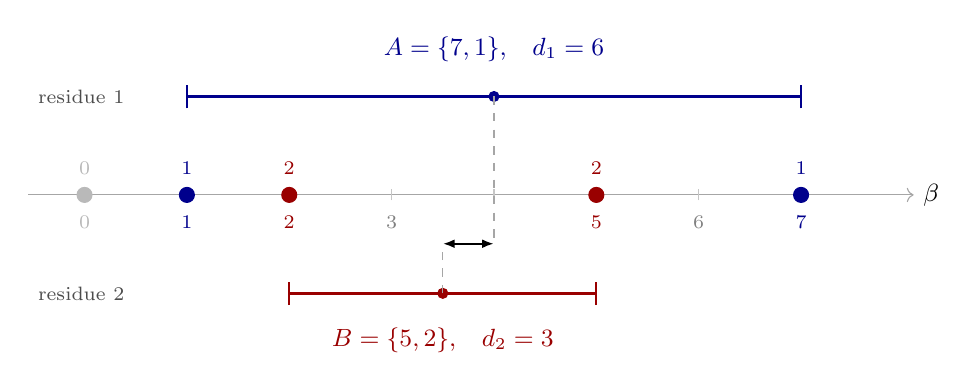
\begin{tikzpicture}[font=\small,x=1.3cm,y=1.0cm]
% --- the two intervals, well clear of the axis ---
\draw[blue!55!black,very thick] (1,1.25) -- (7,1.25);
\draw[blue!55!black,thick] (1,1.10) -- (1,1.40);
\draw[blue!55!black,thick] (7,1.10) -- (7,1.40);
\filldraw[blue!55!black] (4,1.25) circle (1.8pt);
\node[blue!55!black,above=9pt] at (4,1.25) {$A=\{7,1\}$,\quad $d_1=6$};
\draw[red!60!black,very thick] (2,-1.25) -- (5,-1.25);
\draw[red!60!black,thick] (2,-1.40) -- (2,-1.10);
\draw[red!60!black,thick] (5,-1.40) -- (5,-1.10);
\filldraw[red!60!black] (3.5,-1.25) circle (1.8pt);
\node[red!60!black,below=9pt] at (3.5,-1.25) {$B=\{5,2\}$,\quad $d_2=3$};
% --- the beta line ---
\draw[->,gray!70] (-0.55,0) -- (8.1,0) node[right,black]{$\beta$};
\foreach \b in {0,...,7} \draw[gray!45] (\b,-0.07) -- (\b,0.07);
\foreach \b in {3,6} \node[gray,font=\scriptsize,below=4pt] at (\b,0) {$\b$};
\foreach \b/\c/\r in {7/blue!55!black/1, 5/red!60!black/2, 2/red!60!black/2,
                      1/blue!55!black/1, 0/gray!55/0}
  {\filldraw[\c] (\b,0) circle (2.7pt);
   \node[\c,font=\scriptsize,below=4pt] at (\b,0) {$\b$};
   \node[\c,font=\scriptsize,above=4pt] at (\b,0) {$\r$};}
% --- the centres and their distance ---
\draw[gray!70,dashed] (4,1.25) -- (4,-0.62);
\draw[gray!70,dashed] (3.5,-1.25) -- (3.5,-0.62);
\draw[{Latex[length=1.5mm]}-{Latex[length=1.5mm]},thick] (3.5,-0.62) -- (4,-0.62);
\node[font=\scriptsize,gray!60!black,anchor=west] at (-0.55,1.25) {residue $1$};
\node[font=\scriptsize,gray!60!black,anchor=west] at (-0.55,-1.25) {residue $2$};
\end{tikzpicture}
\caption{The mechanism for $t=3$, $\lambda=(3,2)$: here $N=5$, $\beta=(7,5,2,1,0)$ with residues
$(1,2,2,1,0)$ modulo $3$, so no class is empty and two classes have size two. The three arguments of
\eqref{eq:main} are the two interval lengths and twice the distance between the interval centres;
the short double arrow marks that distance, here $\tfrac12$, so that $d_3=1$.}
\label{fig:intervals}
\end{figure}

\begin{example}
For $t=3$, $\lambda=(3,2)$ as in Figure \ref{fig:intervals}, $(d_1,d_2,d_3)=(6,3,1)$ and
\[
\Phi_3\bigl((3,2);z\bigr)=\varepsilon\,
\frac{\sinh(3\theta)\sinh(\theta/2)}{\sinh(3\theta/2)\sinh\theta}.
\]
For $t=3$, $\lambda=(3,1)$ the profile is the size-three one, $(d_1,d_2,d_3)=(3,3,6)$ and
$\Phi_3=\varepsilon\,\chi_2(z)$. For $t=4$, $\lambda=(1,1,1)$ we have $\beta=(6,5,4,2,1,0)$, the
class $3$ is empty and $\Phi_4=0$.
\end{example}

\subsection{The image of the map}
Theorem \ref{thm:main} sends every partition with at most $N$ rows to three integers, so the whole
family collapses onto a sparse subset of $\ZZ^3$. By Proposition \ref{prop:quotient} the first two
coordinates are multiples of $t$; the third is not a multiple of $t$ except in the size-three
profile, where $d_3=d_1+d_2$. Figure \ref{fig:image} shows the image for $t=3$ and $t=4$, coloured
by the number of partitions collapsing onto each point.

\begin{figure}[t]
\centering
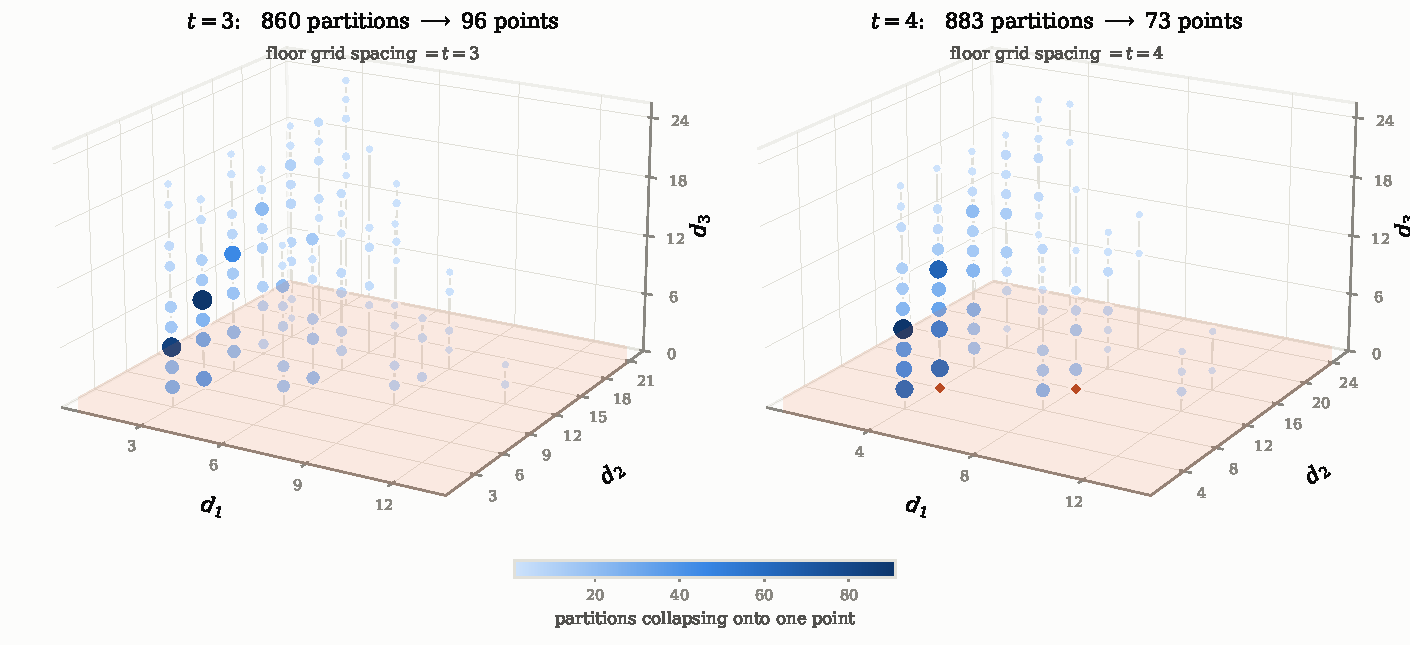
\includegraphics[width=\textwidth]{fig_image.pdf}
\caption{The image of $\lambda\mapsto(d_1,d_2,d_3)$ over all $\lambda$ with $|\lambda|\le20$ and at
most $t+2$ rows, for $t=3$ (left) and $t=4$ (right), taken \emph{up to the exchange of $d_1$ and
$d_2$}, under which \eqref{eq:main} is symmetric; without that identification, and with $A$ and $B$
in the order $r_A\le r_B$ of Theorem \ref{thm:main}, the two panels carry $126$ and $92$ points
rather than $96$ and $73$. The compression is the point of the picture: $860$
partitions land on $96$ triples on the left and $883$ on $73$ on the right, and colour and area give
the number of partitions mapping to each. The floor grid spacing is $t$, since $d_1,d_2\in t\ZZ$ by Proposition
\ref{prop:quotient}; the shaded plane $d_3=0$ is the concentric locus of Corollary \ref{cor:zero},
where $s_\lambda$ vanishes, so those shapes are not in the image and are drawn on the plane as
diamonds instead. The two panels are the two parities, which is the content of Proposition
\ref{rem:lattice}: the odd one carries no diamond, and can carry none; the even one carries two,
between them the images of $32$ partitions.}
\label{fig:image}
\end{figure}

Figure \ref{fig:image} is one half of the picture: it shows which triples occur, not what a triple
hides. Figure \ref{fig:fibres} is the other half. Over each cell of the $(d_1,d_2)$ floor it stands
the column of sizes $|\lambda|$ that land there, so a column is a set of partitions of different
sizes on which $\Phi_t$ takes one and the same value --- and the columns do not thin out as
$|\lambda|$ grows, since the values are confined to a lattice and the partitions are not. The most
visible one is the fibre of the empty partition: at $t=3$ the invariant $I_3=(3,3,2,+1)$ is shared by
$26$ partitions, of $19$ different sizes between $0$ and $20$, so $\Phi_3$ does not distinguish
$\varnothing$ from a shape of twenty boxes.

\begin{figure}[!ht]
\centering
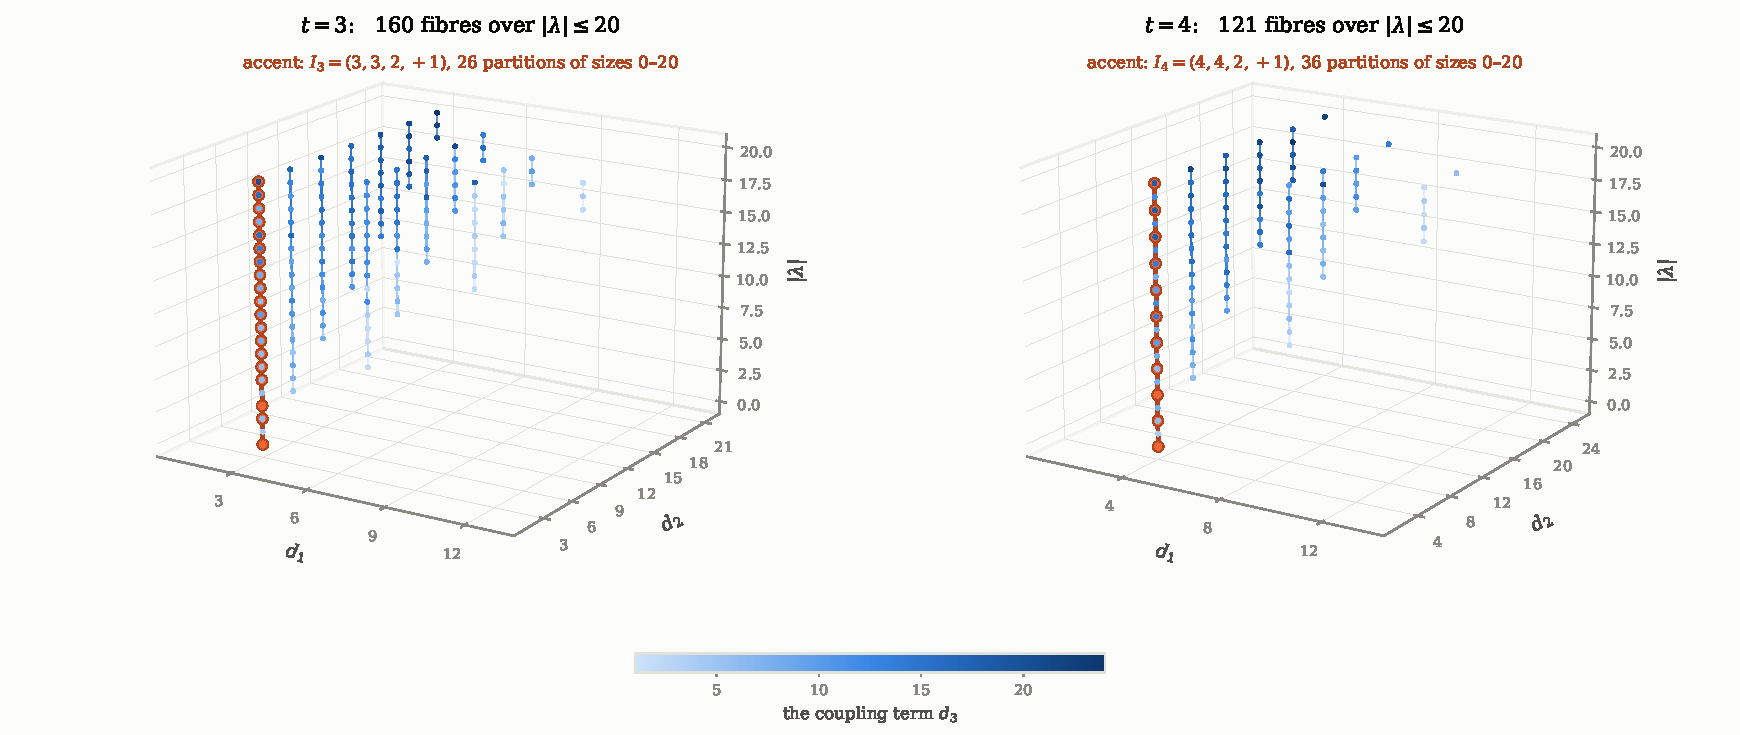
\includegraphics[width=\textwidth]{fig_fibres.pdf}
\caption{The fibres of the evaluation invariant \eqref{eq:invariant}, the complement of Figure
\ref{fig:image}: the same range $|\lambda|\le20$, with the coupling term moved to colour and the
size $|\lambda|$ on the vertical axis. A column is one fibre, so its height is the range of sizes
this alphabet cannot tell apart; the floor ticks are the lattice $t\ZZ$ of Proposition
\ref{prop:quotient}, and only the half $d_1\le d_2$ is occupied because the triple is taken up to the
exchange, as in Figure \ref{fig:image}. That every marker of a column carries the same value is
computed and not assumed: over the $860$ partitions on the left and the $883$ on the right the
bialternant is constant on each fibre to $10^{-37}$. The accent column is the fibre of
$\lambda=\varnothing$.}
\label{fig:fibres}
\end{figure}

Figure \ref{fig:fibres} makes one thing about \eqref{eq:invariant} precise: $I_t$ is complete but
not minimal. The numerator of \eqref{eq:main} is symmetric in $d_1,d_2,d_3$, so the value sees only the multiset
$\{d_1,d_2,d_3\}$ together with the sign, and that is a real reduction --- over $t=4$ and
$|\lambda|\le20$ the $121$ invariants take only $110$ values, while at $t=3$ in the same range the
two counts agree. In the same range no two distinct multisets share a value, so the minimal invariant
of this evaluation is the pair (multiset, sign); we keep the ordered form in \eqref{eq:invariant}
because $d_3$ is the coordinate the reciprocal pair contributes and the other two are not, and
Corollary \ref{cor:fibregf} describes the fibres of either, since the two differ by a symmetry of
the numerator and not by anything the lattice sees.

\begin{proposition}[a shorter form of the sign]\label{rem:sign}
Let the residue profile be non-degenerate and $a_1+a_2\ne b_1+b_2$, and order the two distinguished
classes so that $r_A\le r_B$. Then
\begin{equation}\label{eq:shortsign}
\boxed{\;\;\varepsilon_\lambda\;=\;(-1)^{\lfloor t/2\rfloor}\,\sgn(\sigma)\,(-1)^{\,r_A+r_B}\,
\sgn\bigl(a_1+a_2-b_1-b_2\bigr)\;\;}
\end{equation}
where $\sigma$ is the permutation of \S\ref{sec:background}.
\end{proposition}

\begin{proof}
Let $w$ be the residue word of $\beta(\lambda)$ read in increasing column order. Since $\beta$
decreases with the column index, grouping the parts by class with the values decreasing inside each
class is the stable sort of $w$, so $\sgn(\sigma)=(-1)^{\inv(w)}$. Both sides of
\eqref{eq:shortsign} carry the factor $\sgn(a_1+a_2-b_1-b_2)$, and
$\sgn(a_1-b_1)=(-1)^{[a_1<b_1]}$, so by \eqref{eq:sign} the assertion is equivalent to
\begin{equation}\label{eq:signparity}
j_{A_1}+j_{B_1}+\inv(w)+\inv(b_S)+[a_1<b_1]\;\equiv\;
\Bigl\lfloor\tfrac t2\Bigr\rfloor+t+\binom{N+1}{2}+r_A+r_B \pmod 2 .
\end{equation}

We use one parity count. Let $u$ be a word, $p$ a position, $c=u_p$, and let $I(p)$ be the number of
inversions of $u$ in which $p$ takes part; write $\nu_{<c}$ for the number of letters of $u$ strictly
below $c$ and $e_p$ for the number of occurrences of $c$ strictly before $p$. Putting
$x=\#\{j<p:u_j>c\}$, the positions before $p$ split as $p-1=x+e_p+\#\{j<p:u_j<c\}$ and the letters
below $c$ split as $\nu_{<c}=\#\{j<p:u_j<c\}+\#\{j>p:u_j<c\}$, whence
\begin{equation}\label{eq:parity}
I(p)\;=\;x+\#\{j>p:u_j<c\}\;=\;2x+e_p+\nu_{<c}-(p-1)\;\equiv\;(p-1)+\nu_{<c}+e_p \pmod 2 .
\end{equation}
Since $b_S$ is $w$ with the letters at the positions $j_{A_1}$ and $j_{B_1}$ deleted,
\[
\inv(w)-\inv(b_S)=I(j_{A_1})+I(j_{B_1})
-\bigl[\,\{j_{A_1},j_{B_1}\}\ \text{is an inversion of }w\,\bigr],
\]
and $\inv(w)+\inv(b_S)\equiv\inv(w)-\inv(b_S)$, so \eqref{eq:parity} computes the left-hand side of
\eqref{eq:signparity}.

In the two-class profile $r_A<r_B$, and $w$ carries $r_A$ twice, $r_B$ twice and every other residue
once. Because $\beta$ decreases with the column index, $a_1>a_2$ puts $j_{A_1}$ at the \emph{first}
occurrence of $r_A$, so $e=0$ there, and likewise at $j_{B_1}$. The letters below $r_A$ are one copy
of each of $0,\dots,r_A-1$, so $\nu_{<r_A}=r_A$; those below $r_B$ are the same together with the
second copy of $r_A$, so $\nu_{<r_B}=r_B+1$. The two positions form an inversion exactly when the
larger letter comes first, that is when $j_{B_1}<j_{A_1}$, that is when $a_1<b_1$. Hence
\[
\inv(w)-\inv(b_S)\;\equiv\;(j_{A_1}-1+r_A)+(j_{B_1}-1+r_B+1)+[a_1<b_1]
\;\equiv\;j_{A_1}+j_{B_1}+r_A+r_B+1+[a_1<b_1],
\]
and substituting this in \eqref{eq:signparity} cancels the columns and $[a_1<b_1]$ in pairs, leaving
$\lfloor t/2\rfloor+t+\binom{N+1}{2}\equiv1$.

In the size-three profile $r_A=r_B=:r$ and the class $\{p>q>p'\}$ sits at columns $j_1<j_2<j_3$ with
$A=\{p,q\}$ and $B=\{q,p'\}$, so $j_{A_1}=j_1$ and $j_{B_1}=j_2$ carry the same letter $r$, with
$e=0$ and $e=1$ respectively and $\nu_{<r}=r$ in both; two equal letters are not an inversion, and
$a_1>b_1$. So $\inv(w)-\inv(b_S)\equiv j_1+j_2+1$, which is the displayed expression again because
$r_A+r_B=2r$ and $[a_1<b_1]=0$, and \eqref{eq:signparity} reduces to the same congruence.

Finally $N=t+2$, so that congruence reads $\lfloor t/2\rfloor+t+\binom{t+3}{2}\equiv1$: for $t=2m$
its three terms are $m$, $0$ and $m+1$, and for $t=2m+1$ they are $m$, $1$ and $m$. Both sums are
odd, and the identity holds for every $t\ge2$.
\end{proof}

The ordering by residue is not a convenience, and it is worth saying why. Exchanging the two blocks
negates the sign $\kappa_{11}$ of Lemma \ref{lem:L4} --- through its $\sgn(a_1-b_1)$ factor --- and negates
$\sgn(a_1+a_2-b_1-b_2)$ as well, so it leaves $\varepsilon_\lambda$, which is their product,
invariant; as it must, since $\varepsilon_\lambda$ is attached to $\lambda$. The right-hand side
above is \emph{not} invariant: $(-1)^{r_A+r_B}$ is symmetric, so only its last factor changes sign.
Without a rule fixing which block is $A$, the right-hand side is therefore not a function of
$\lambda$ at all. The hypothesis enters the proof at one point and one only: it is what makes
$\nu_{<r_A}=r_A$ and $\nu_{<r_B}=r_B+1$ rather than the other way round, and dropping it exchanges
those two counts and breaks \eqref{eq:signparity}.

Read the other way round, \eqref{eq:shortsign} says that $\Phi_t$ is a function of a small
combinatorial datum and of nothing else, and it says so for every $t$ rather than over a range: by
Theorem \ref{thm:main} the triple $(d_1,d_2,d_3)$ determines $\Phi_t$ up to sign, and adjoining
$\sgn(\sigma)$, the ordered pair $r_A\le r_B$ and the \emph{orientation}
$\sgn(a_1+a_2-b_1-b_2)$ of $d_3$ determines it outright. The shape of $\lambda$ enters nowhere else.
The orientation is not optional, and that part remains a check rather than a proof: over $t\le6$ and
$|\lambda|\le14$, putting $\sgn(a_1-b_1)$ in its place leaves collisions at $t=2$.

%======================================================================
\section{Proof of Theorem \ref{thm:main}}\label{sec:proof}

The proof uses the Vandermonde determinant, the Laplace expansion, and one cancellation lemma. We
give the steps separately so that a reader checking the ancillary scripts can localise any
disagreement.

What the argument really does is classify rather than compute. Expanding along the $t$ frozen rows
leaves one term for each way of choosing which two columns are \emph{not} frozen, and the excess-two
count says every such choice falls into exactly one of three combinatorial types: none survives
(a residue class is empty), four survive (two classes of size two), or three do (one class of size
three). Everything after that is bookkeeping inside a type, and Lemma \ref{lem:L5} shows the last two
types are one statement seen twice.

\begin{lemma}\label{lem:L1}
Let $S$ be a set of $t$ columns and $M_S=\det(\zeta^{k\beta_j})_{0\le k<t,\,j\in S}$. Then $M_S=0$
unless the residues $\{\beta_j\bmod t:j\in S\}$ are pairwise distinct, in which case
$M_S=(-1)^{\inv(b_S)}V$.
\end{lemma}

\begin{proof}
Since $\zeta^{k\beta_j}=(\zeta^{\beta_j})^k$, the matrix is a Vandermonde matrix in the values
$y_j=\zeta^{\beta_j}$, whose determinant is $\prod_{j<j'}(y_{j'}-y_j)$. The value $y_j$ depends on
$\beta_j$ only modulo $t$, so two columns of $S$ sharing a residue make the determinant vanish. If
the residues are pairwise distinct then $|S|=t$ forces $\{y_j\}_{j\in S}=\zt$ as a set, and the
Vandermonde determinant is alternating in its arguments, so it equals $V$ times the sign of the
permutation sorting $b_S$ increasingly, which is $(-1)^{\inv(b_S)}$.
\end{proof}

\begin{lemma}\label{lem:L2}
$\det\bigl(x_i^{N-j}\bigr)_{i,j=1}^{N}
=(-1)^{\binom t2}\,V\,(z^t-1)(z^{-t}-1)(z-z^{-1})$ for the alphabet
$x=(1,\zeta,\dots,\zeta^{t-1},z,z^{-1})$ in that order.
\end{lemma}

\begin{proof}
The determinant is $\prod_{i<i'}(x_i-x_{i'})$. Pairs inside $\zt$ contribute
$\prod_{k<k'}(\zeta^k-\zeta^{k'})=(-1)^{\binom t2}V$; pairs $(\zeta^k,z)$ contribute
$\prod_k(\zeta^k-z)=(-1)^t(z^t-1)$ and pairs $(\zeta^k,z^{-1})$ contribute $(-1)^t(z^{-t}-1)$; the
last pair contributes $z-z^{-1}$. The two factors $(-1)^t$ cancel.
\end{proof}

\begin{lemma}\label{lem:L3}
Let $\mathcal U$ be the set of pairs $U=\{j_1<j_2\}$ of columns whose complement $S_U$ carries all
$t$ residues. Then
\[
\Phi_t(\lambda;z)=\frac{(-1)^{\,t+\binom{N+1}{2}}}{(z^t-1)(z^{-t}-1)(z-z^{-1})}
\sum_{U\in\mathcal U}(-1)^{\,j_1+j_2+\inv(b_{S_U})}\,f(\beta_{j_1}-\beta_{j_2}).
\]
\end{lemma}

\begin{proof}
Expanding the numerator by Laplace along the first $t$ rows,
\[
\det\bigl(x_i^{\beta_j}\bigr)=\sum_{|S|=t}(-1)^{\binom{t+1}{2}+\sum_{j\in S}j}\,M_S\,C_{S^c},
\]
where for $S^c=\{j_1<j_2\}$ the complementary $2\times2$ minor is
$z^{\beta_{j_1}-\beta_{j_2}}-z^{-(\beta_{j_1}-\beta_{j_2})}=f(\beta_{j_1}-\beta_{j_2})$. By Lemma
\ref{lem:L1} only $S$ with pairwise distinct residues contribute. Writing
$\sum_{j\in S}j=\binom{N+1}{2}-j_1-j_2$ and dividing by Lemma \ref{lem:L2}, the factors $V$ cancel
and $(-1)^{\binom{t+1}{2}-\binom{t}{2}}=(-1)^t$.
\end{proof}

If some $n_i=0$ then no $S$ of size $t$ carries all residues, $\mathcal U=\varnothing$, and
$\Phi_t=0$: this is Theorem \ref{thm:main}(i). Otherwise all $n_i\ge1$ and by \eqref{eq:excess}
either two classes have size two, in which case $S_U$ must drop one element of each and
$|\mathcal U|=4$, or one class has size three, in which case $S_U$ drops two of the three and
$|\mathcal U|=3$.

\begin{lemma}[the column move]\label{lem:L4}
Let $A$ and $B$ be distinct classes of size two, at columns $j_{A_1}<j_{A_2}$ and
$j_{B_1}<j_{B_2}$. For $i,j\in\{1,2\}$ let $U_{ij}$ consist of the column of $a_i$ and the column of
$b_j$, and set $\kappa_{ij}=(-1)^{\,j_{A_i}+j_{B_j}+\inv(b_{S_{U_{ij}}})}\sgn(a_i-b_j)$, so that
the $U_{ij}$ term of Lemma \ref{lem:L3} equals $\kappa_{ij}f(a_i-b_j)$. Then
$\kappa_{ij}=\kappa_{11}(-1)^{i-1}(-1)^{j-1}$.
\end{lemma}

\begin{proof}
Fix $j$ and compare $i=1$ with $i=2$. The sets $S_{U_{1j}}$ and $S_{U_{2j}}$ differ only in that the
first contains the column $j_{A_2}$ and the second the column $j_{A_1}$, and the letter carried is
the residue $r_A$ in both. Passing from one word to the other moves that letter across exactly the
kept columns strictly between $j_{A_1}$ and $j_{A_2}$, and none of those letters equals $r_A$
because the class $A$ has only two elements; each crossing changes the parity of $\inv$. Hence
\[
(-1)^{\inv(b_{S_{U_{1j}}})-\inv(b_{S_{U_{2j}}})}
=(-1)^{(j_{A_2}-j_{A_1}-1)-[\,a_2<b_j<a_1\,]},
\]
using that $\beta$ is strictly decreasing in the column index, so that $j_{B_j}$ lies strictly
between $j_{A_1}$ and $j_{A_2}$ exactly when $a_2<b_j<a_1$. Multiplying by the Laplace factor
$(-1)^{j_{A_1}+j_{A_2}}$,
\[
\frac{\kappa_{1j}}{\kappa_{2j}}
=(-1)^{2j_{A_2}-1}(-1)^{[\,a_2<b_j<a_1\,]}\sgn(a_1-b_j)\sgn(a_2-b_j)=-1,
\]
because $\sgn(a_1-b_j)\sgn(a_2-b_j)=-1$ exactly when $b_j$ lies between $a_2$ and $a_1$. Exchanging
the roles of $A$ and $B$ gives $\kappa_{i1}/\kappa_{i2}=-1$.
\end{proof}

\begin{lemma}\label{lem:L5}
For all $c,p,q$ and all $u,v$,
\begin{align*}
\text{\rm(a)}&\quad \sum_{\epsilon,\eta\in\{\pm1\}}\epsilon\eta\,f(c+\epsilon p+\eta q)=f(c)f(p)f(q),\\
\text{\rm(b)}&\quad f(2u)-f(2u+2v)+f(2v)=-f(u)f(v)f(u+v).
\end{align*}
\end{lemma}

\begin{proof}
For (a), $\sum_{\epsilon,\eta}\epsilon\eta\,z^{c+\epsilon p+\eta q}
=z^{c}\bigl(\sum_\epsilon\epsilon z^{\epsilon p}\bigr)\bigl(\sum_\eta\eta z^{\eta q}\bigr)
=z^{c}f(p)f(q)$, and the same computation for the negative exponents gives
$z^{-c}(-f(p))(-f(q))$; subtract. For (b), put $s=z^u$, $w=z^v$ and expand
$(s-s^{-1})(w-w^{-1})(sw-s^{-1}w^{-1})$: the eight terms recombine as
$(s^2w^2-s^{-2}w^{-2})-(s^2-s^{-2})-(w^2-w^{-2})=f(2u+2v)-f(2u)-f(2v)$.
\end{proof}

\begin{proof}[Proof of Theorem \ref{thm:main}]
In the two-class profile, Lemmas \ref{lem:L3} and \ref{lem:L4} give
\[
\sum_{U\in\mathcal U}(\cdots)=\kappa_{11}\sum_{i,j}(-1)^{i-1}(-1)^{j-1}f(a_i-b_j).
\]
Writing $a_i=\alpha+\epsilon_ip$ and $b_j=\gamma+\eta_jq$ with $p=d_1/2$, $q=d_2/2$ and
$\epsilon=\eta=(+1,-1)$, we have $a_i-b_j=c+\epsilon_ip-\eta_jq$ with $c=\alpha-\gamma$. Replacing
$\eta$ by $-\eta$ turns the sum into $-\sum_{\epsilon,\eta}\epsilon\eta f(c+\epsilon p+\eta q)$,
which is $-f(c)f(p)f(q)$ by Lemma \ref{lem:L5}(a). Since
$(z^t-1)(z^{-t}-1)=2-z^t-z^{-t}=-f(t/2)^2$ and $z-z^{-1}=f(1)$, the two minus signs cancel, and
substituting $f(u)=2\sinh(u\theta)$ the numerical factors cancel and
$\sinh(c\theta)=\sgn(c)\sinh(d_3\theta/2)$, giving \eqref{eq:main} with
$\varepsilon_\lambda=(-1)^{\,t+\binom{N+1}{2}}\kappa_{11}\sgn(a_1+a_2-b_1-b_2)$, which is
\eqref{eq:sign} by the definition of $\kappa_{11}$ in Lemma \ref{lem:L4}.

For the size-three profile $\{p>q>r\}$ at columns $j_1<j_2<j_3$ the same column-move argument
applies, again because no letter strictly between two of these columns carries the class residue,
and gives alternating signs $(\varsigma,-\varsigma,\varsigma)$ for the three terms $f(p-q)$,
$f(p-r)$, $f(q-r)$. By Lemma \ref{lem:L5}(b) with $u=(p-q)/2$, $v=(q-r)/2$ the sum is
$-\varsigma f(u)f(v)f(u+v)$, which is the two-class formula for $A=\{p,q\}$, $B=\{q,r\}$ with
$\varsigma=\kappa_{11}$. Equivalently, the missing fourth selection of the two-class profile would
drop $q$ twice and its term carries $f(0)=0$, so the two profiles are one statement.
\end{proof}

All the statements of this paper were also checked numerically; the counts are collected once, in
\S\ref{sec:verif}, rather than repeated as they arise.

%======================================================================
\section{Independence on the reciprocal locus}\label{sec:independence}

Specializing \eqref{eq:AK53} as in \S\ref{sec:background} gives: for $\ell(\lambda)\le2$,
$s_\lambda(z,\zb,\zt)=s_\lambda(z,\zb)$ if and only if $\lambda=\core_t(\lambda)$. Theorem
\ref{thm:main} evaluates the left-hand side for every $\lambda$, and comparing the two shows that on
the reciprocal locus the criterion acquires further solutions --- exactly one family.

We first isolate when $\Phi_t$ degenerates to a single character. Recall
$\chi_k(z)=(z^{k+1}-z^{-k-1})/(z-z^{-1})$.

\begin{lemma}\label{lem:single}
$\Phi_t(\lambda;z)=\pm\chi_k(z)$ for some $k\ge0$ if and only if the multiset $\{d_1,d_2,d_3\}$
contains $t$ at least twice, and in that case the remaining entry equals $2(k+1)$.
\end{lemma}

\begin{proof}
Put $u=z^{1/2}$, so that $2\sinh(d_i\theta/2)=u^{d_i}-u^{-d_i}$, $2\sinh(t\theta/2)=u^{t}-u^{-t}$ and
$2\sinh\theta=u^{2}-u^{-2}$; all exponents are integers. By \eqref{eq:main}, the asserted equality is
\[
\prod_{i=1}^{3}\bigl(u^{d_i}-u^{-d_i}\bigr)
=\pm\bigl(u^{t}-u^{-t}\bigr)^{2}\bigl(u^{2k+2}-u^{-2k-2}\bigr).
\]
Using $u^{n}-u^{-n}=u^{-n}(u^{2n}-1)$ on each factor and comparing the monomial prefactors gives
$d_1+d_2+d_3=2t+2(k+1)$ together with
\[
\prod_{i=1}^{3}\bigl(u^{2d_i}-1\bigr)=\pm\bigl(u^{2t}-1\bigr)^{2}\bigl(u^{4(k+1)}-1\bigr),
\]
and evaluating at $u=0$ fixes the sign to $+$. Now $u^{2n}-1=\prod_{m\mid 2n}\Phi_m(u)$ with
$\Phi_m$ the cyclotomic polynomials, which are irreducible and pairwise distinct, so by unique
factorization in $\ZZ[u]$ the two sides have the same multiset of cyclotomic factors. On the left
that multiset is $\biguplus_i\{m:m\mid 2d_i\}$ and on the right it is
$2\times\{m:m\mid 2t\}\uplus\{m:m\mid 4(k+1)\}$. Its largest element is $\max_i 2d_i$ on the left and
$\max(2t,4(k+1))$ on the right; deleting the divisor set of that maximum from both sides and
repeating twice more yields
\[
\{2d_1,2d_2,2d_3\}=\{2t,\,2t,\,4(k+1)\}
\]
as multisets, which is the assertion. The converse is the same computation read backwards.
\end{proof}

\begin{theorem}\label{thm:extra}
Let $\ell(\lambda)\le2$. Then $\Phi_t(\lambda;z)=\pm s_\lambda(z,\zb)$ if and only if either
$\lambda=\core_t(\lambda)$, or
\begin{equation}\label{eq:extra}
t\ \text{is even}\quad\text{and}\quad \lambda=\Bigl(\lambda_2+\tfrac{3t}{2}-1,\ \lambda_2\Bigr)
\quad\text{with}\quad \tfrac t2\le\lambda_2\le t-1 .
\end{equation}
In the second case $\{d_1,d_2,d_3\}=\{3t,t,t\}$, while $\core_t(\lambda)=\bigl(\tfrac t2-1+j,j\bigr)$
and $\quot_t(\lambda)$ has the single nonempty component $(2)$, in slot $j=\lambda_2-\tfrac t2$.
\end{theorem}

Figure \ref{fig:locus} is the statement computed rather than asserted: both families are plotted
over a range of $t$, and the odd $t$ where \eqref{eq:extra} cannot occur is drawn as the control.

\begin{figure}[!ht]
\centering

\includegraphics[width=\textwidth]{fig_locus.pdf}
\caption{Theorem \ref{thm:extra}, computed rather than asserted. For every two-row $\lambda$ in
range, both sides of $\Phi_t(\lambda;z)=\pm s_\lambda(z,\zb)$ were evaluated; the partitions where
they agree are plotted and coloured by family. Circles are the $t$-cores, the solutions already
described by \eqref{eq:AK53}; triangles are the extra family \eqref{eq:extra}, which the reciprocal
specialization creates. The odd case $t=3$ is the control: by Theorem \ref{thm:extra} no extra
solution can exist there, and none is found.}
\label{fig:locus}
\end{figure}

\begin{proof}
Since $\ell(\lambda)\le 2$ and $N=t+2$, the beta set is
$\beta(\lambda)=\bigl(A'+t,\;B'+t,\;t-1,t-2,\dots,1,0\bigr)$ where
\[
A':=\lambda_1+1,\qquad B':=\lambda_2,\qquad A'>B'\ge0 .
\]
The block $\{0,1,\dots,t-1\}$ meets every residue class exactly once, so no class is empty and the
two large parts decide the profile. Write $A'=t\alpha+\rho_A$ and $B'=t\gamma+\rho_B$ with
$0\le\rho_A,\rho_B\le t-1$. As $s_\lambda(z,\zb)=\chi_{\lambda_1-\lambda_2}(z)$, Lemma
\ref{lem:single} says that the assertion holds precisely when $\{d_1,d_2,d_3\}$ contains $t$ twice
and the third entry is $2(\lambda_1-\lambda_2+1)=2(A'-B')$.

\emph{Case $\rho_A=\rho_B=:\rho$.} One class has size three, namely $\{A'+t,B'+t,\rho\}$, and by
Theorem \ref{thm:main} the three arguments are
$d_1=A'-B'$, $d_2=B'+t-\rho=t(\gamma+1)$, $d_3=A'+t-\rho=t(\alpha+1)$. Here $t\mid A'-B'$, say
$A'-B'=ts$ with $s\ge1$. The pair $d_2=d_3=t$ forces $\alpha=\gamma=0$, hence $A'=B'$, excluded.
The pair $d_1=d_3=t$ forces $s=1$ and $\alpha=0$, hence $A'<t$ and $A'=B'+t\ge t$, excluded. The pair
$d_1=d_2=t$ forces $s=1$ and $\gamma=0$, i.e. $A'=B'+t$ with $B'<t$; then $\alpha=1$ and the third
entry is $d_3=2t=2(A'-B')$, as required. So this case contributes exactly the $\lambda$ with
$A'=B'+t$, $B'<t$.

\emph{Case $\rho_A\ne\rho_B$.} Two classes have size two, namely $\{A'+t,\rho_A\}$ and
$\{B'+t,\rho_B\}$, and the three arguments are
\[
d_A=t(\alpha+1),\qquad d_B=t(\gamma+1),\qquad
d_3=\bigl|\,t(\alpha-\gamma)+2(\rho_A-\rho_B)\,\bigr| .
\]
If $d_A=d_B=t$ then $\alpha=\gamma=0$, so $A',B'<t$ and $d_3=2|\rho_A-\rho_B|=2(A'-B')$
automatically: every such $\lambda$ is a solution. Otherwise exactly one of $d_A,d_B$ equals $t$ and
$d_3=t$. If $\alpha=0$ and $\gamma\ge1$ then $|-t\gamma+2(\rho_A-\rho_B)|=t$ with
$|\rho_A-\rho_B|\le t-1$ forces $\gamma=2$ and $\rho_A-\rho_B=t/2$; but then
$\lambda_1=A'-1=\rho_A-1<t$ while $\lambda_2=B'\ge2t$, contradicting $\lambda_1\ge\lambda_2$. If
$\gamma=0$ and $\alpha\ge1$ then $|t\alpha+2(\rho_A-\rho_B)|=t$ forces, for $\alpha=1$,
$\rho_A=\rho_B$ (excluded), and for $\alpha=2$,
\[
\rho_B-\rho_A=\tfrac t2,
\]
which requires $t$ even; $\alpha\ge3$ gives $|2(\rho_A-\rho_B)|\ge2t$, impossible. So $A'=2t+\rho_A$,
$B'=\rho_B=\rho_A+\tfrac t2$, whence
\[
\lambda_1=2t+\rho_A-1,\qquad \lambda_2=\rho_A+\tfrac t2,\qquad
\lambda_1-\lambda_2=\tfrac{3t}{2}-1,
\]
and $\rho_B\le t-1$ gives $0\le\rho_A\le\tfrac t2-1$, i.e. $\tfrac t2\le\lambda_2\le t-1$. The
remaining entry is $d_A=t(\alpha+1)=3t=2(\lambda_1-\lambda_2+1)$, as required. This is
\eqref{eq:extra}.

It remains to identify the solutions collected in the first case of each analysis with the
$t$-cores. For $\ell(\lambda)\le2$ the beta set in two slots is $(A',B')$, and $\lambda$ is a
$t$-core if and only if neither beta number can be lowered by $t$ into an unoccupied nonnegative
position, i.e. if and only if $B'<t$ and either $A'<t$ or $A'=B'+t$. These are exactly the two
families found above. Finally, in case \eqref{eq:extra} the class $\rho_A$ carries
$\{2t+\rho_A+t,\rho_A\}$, so its quotient component is $(2)$, every other component is empty, and
the core is as stated.
\end{proof}


\begin{remark}\label{rem:why}
Theorem \ref{thm:extra} is stated up to sign because that is what Lemma \ref{lem:single} controls;
over two-row shapes with $t\le8$ the sign is $+1$ at every solution, so there the equality holds on
the nose.

The extra family belongs to the specialization rather than to the alphabet. The step is
\cite[Lemma 5.2]{AK25}, on which \cite[Theorem 5.3]{AK25} rests: it reduces the independence to the
vanishing of $s_{\lambda/\mu}$ at the twisted alphabet for all $\mu\subsetneq\lambda$, and the
reduction uses the linear independence of the universal characters $f_\mu$ in the free variables. On the reciprocal locus $s_\mu(z,\zb)=\chi_{\mu_1-\mu_2}(z)$
depends only on $\mu_1-\mu_2$, so $s_{(1)}$, $s_{(2,1)}$ and $s_{(3,2)}$ agree there and that
independence is not available; Theorem \ref{thm:extra} measures the difference. A control confirms
the reading: for $\lambda=(3,1)$ and $t=2$ one has $s_\lambda(\zt,z,\zb)=s_\lambda(z,\zb)$, while
$s_\lambda(\zt,x,y)\ne s_\lambda(x,y)$ for free $x,y$.
\end{remark}

So the criterion does not survive the specialization unchanged, and what it acquires is small and
nameable: one family, for two-row shapes, indexed by an order-two element of the residue lattice and
classified by its core and quotient. The extra solutions belong to the reciprocal locus, not to the
alphabet --- they exist because a specialization has removed a linear independence the original
argument used, and that missing step is exactly what Theorem \ref{thm:extra} measures.

%======================================================================
\section{An enumeration in which a parameter survives}\label{sec:enum}

Expanding $s_\lambda$ over semistandard tableaux turns Theorem \ref{thm:main} into a product formula
for a weighted count. Let $m_k(T)$ be the number of entries equal to $k$ in $T$.

\begin{corollary}\label{cor:enum}
Expanding $s_\lambda$ over semistandard tableaux and applying Theorem \ref{thm:main}: for every
$t\ge2$ and every $\lambda\in\PP_{t+2}$,
\[
\sum_{T\in\mathrm{SSYT}(\lambda,\,t+2)}
\zeta^{\,\sum_{k=1}^{t}(k-1)m_k(T)}\;z^{\,m_{t+1}(T)-m_{t+2}(T)}
\;=\;\varepsilon_\lambda\,
\frac{\sinh(d_1\theta/2)\sinh(d_2\theta/2)\sinh(d_3\theta/2)}{\sinh^2(t\theta/2)\sinh\theta}.
\]
\end{corollary}

For $t=2$ the weight is $(-1)^{m_2(T)}$, and if $\lambda=(c^r)$ is rectangular then
$\mathrm{SSYT}(\lambda,4)$ is in bijection with plane partitions in an $r\times(4-r)\times c$ box,
equivalently with lozenge tilings of a hexagon. Corollary \ref{cor:enum} is then a
$(-1)$-enumeration of those objects \emph{refined by a free parameter} $z$, which records the
difference between the numbers of entries $3$ and $4$. Setting $z=1$ recovers the plain signed
count, which by \eqref{eq:main} equals $\pm d_1d_2d_3/(2t^2)$: for $r=2$, $c=2$ it is $4$; for
$r=2$, $c=4$ it is $9$; for $r=3$, $c=3$ it is $-6$.

\begin{example}\label{ex:boxes}
Taking $\lambda=(c^{\,r})$ with $1\le r\le4$ and $t=2$, the shape has at most four rows, the tableaux
are the plane partitions in an $r\times(4-r)\times c$ box, and the closed form gives the signed
counts of Figure \ref{fig:signed}. Reading it off:
\[
\begin{array}{ll}
1\times3\times c: & \bigl\lfloor (c+2)^2/4\bigr\rfloor,\\[2pt]
2\times2\times c: & (c/2+1)^2 \text{ for } c \text{ even},\qquad 0 \text{ for } c \text{ odd},\\[2pt]
3\times1\times c: & (-1)^c\bigl\lfloor (c+2)^2/4\bigr\rfloor,\\[2pt]
4\times0\times c: & (-1)^c .
\end{array}
\]
The third row is the transpose of the first, which is why the magnitudes agree; the fourth is the
degenerate box, where $s_{(c^4)}(x)=(x_1x_2x_3x_4)^c$ and the alphabet has determinant $-1$. We do
not claim these particular counts as new --- the boxes are small and the sign here is the
specialization $x_2=-1$, not the complementation sign of Kuperberg's $(-1)$-enumerations --- and we
record them only to show what the theorem produces. What does appear to be new is that each of them
is the $z\mapsto1$ value of a one-parameter refinement with the same product formula.
\end{example}

The perfect squares in Example \ref{ex:boxes} are not an accident of small cases: they are what the
interval reading of \S\ref{sec:intervals} says a rectangle must produce.

\begin{proposition}\label{prop:rect}
Let $t=2$ and $\lambda=(c^{\,r})$ with $1\le r\le4$. Then one of $d_1,d_2,d_3$ equals $2$, and:
\begin{enumerate}
\item[\rm(i)] if $r=4$, all three equal $2$ for \emph{every} $c$ and the count is $(-1)^c$; this is
the full rectangle, where $s_{(c^4)}(x)=(x_1x_2x_3x_4)^{c}$ collapses to a monomial and the alphabet
contributes only its determinant;
\item[\rm(ii)] if $r\le3$ and $c$ is even, the other two are both equal to $c+2$, so the two
intervals have the \emph{same length} and the signed count is the perfect square
$\bigl(\tfrac{c+2}{2}\bigr)^2$;
\item[\rm(iii)] if $c$ is odd and $r=2$, the two intervals are \emph{concentric} and the count is $0$;
\item[\rm(iv)] if $c$ is odd and $r\in\{1,3\}$, the other two are $c+1$ and $c+3$, and the count is
$\pm\tfrac{(c+1)(c+3)}{4}=\pm\bigl\lfloor\tfrac{(c+2)^2}{4}\bigr\rfloor$.
\end{enumerate}
Case {\rm(i)} is not a degeneration of the interval triple but a collapse of the shape itself, and it
is the only case in which the parity of $c$ plays no role.
\end{proposition}

\begin{proof}
For $\lambda=(c^{\,r})$ the beta set consists of two blocks of consecutive integers, namely
$c+3,c+2,\dots,c+4-r$ and $3-r,2-r,\dots,0$; residues alternate along each block, which is what
forces the coincidences. Explicitly, for $r=1,2,3,4$ the beta set is $(c+3,2,1,0)$, $(c+3,c+2,1,0)$,
$(c+3,c+2,c+1,0)$ and $(c+3,c+2,c+1,c)$. Splitting each by parity gives, for $c$ even,
\[
\{c{+}3,1\},\{2,0\};\qquad \{c{+}3,1\},\{c{+}2,0\};\qquad \{c{+}3,c{+}1\},\{c{+}2,0\};\qquad
\{c{+}3,c{+}1\},\{c{+}2,c\},
\]
whence $(d_1,d_2,d_3)$ equals $(c{+}2,2,c{+}2)$, $(c{+}2,c{+}2,2)$, $(2,c{+}2,c{+}2)$ and
$(2,2,2)$ respectively; in each case the product over $2t^2=8$ is $\bigl(\tfrac{c+2}{2}\bigr)^2$,
resp. $1$. For $c$ odd and $r=2$ the split is $\{c{+}3,0\},\{c{+}2,1\}$, so
$d_3=|c{+}3+0-c{-}2-1|=0$: the intervals are concentric and Corollary \ref{cor:zero} applies. For
$c$ odd and $r=1,3$ the parity puts three beta numbers in one class, $\{c{+}3,2,0\}$ and
$\{c{+}3,c{+}1,0\}$ respectively, and the size-three profile gives $(c{+}1,2,c{+}3)$ and
$(2,c{+}1,c{+}3)$, with product over $8$ equal to $\tfrac{(c+1)(c+3)}{4}$. For $c$ odd and $r=4$ the
four beta numbers are again consecutive, so the split is $\{c{+}3,c{+}1\},\{c{+}2,c\}$ and the triple
is $(2,2,2)$ exactly as for $c$ even: at full height the answer does not see the parity of $c$, which
is why $r=4$ is separated out.
\end{proof}

So the square is the square of half the common interval length, the zeros are the concentric
configurations, the quarter-squares are the case where the two lengths differ by $2$, and at full
height all three intervals coincide, the shape becomes a monomial and only a sign survives. Which
pair of the three coincides rotates with $r$, which is why the same value appears in different
columns of Figure \ref{fig:signed}.

\begin{figure}[t]
\centering

\includegraphics[width=\textwidth]{fig_signed.pdf}
\caption{The signed counts of Example \ref{ex:boxes}: the value of Corollary \ref{cor:enum} at
$z=1$ and $t=2$ for the rectangular shapes $\lambda=(c^{\,r})$, that is the $(-1)$-enumeration of
plane partitions in an $r\times(4-r)\times c$ box. Every entry is the closed form
$\varepsilon_\lambda\,d_1d_2d_3/(2t^2)$, cross-checked against a direct enumeration of the tableaux.
The row $r=2$ vanishes for odd $c$ and is a perfect square for even $c$.}
\label{fig:signed}
\end{figure}

The $(-1)$-enumeration literature --- Kuperberg \cite{Kup02}, Eisenk\"olbl \cite{Eis07} building on
Stanley \cite{Sta86} and on the Pfaffian identities of \cite{IOTZ06}, Ciucu, Krattenthaler ---
computes such signed counts with the variables specialized to $1$. Keeping the parameter free appears not to have
been recorded, and it is the feature that distinguishes the present alphabet: the reciprocal pair is
precisely the mechanism that lets one variable survive the signed enumeration.

A refinement of a different kind is standard in the ribbon world, and it is worth saying which:
the LLT polynomials of Lascoux, Leclerc and Thibon \cite{LLT97} grade ribbon tableaux by a spin
statistic. That $q$ is an extra grading rather than a letter, and the object it grades is indexed by
a tuple of shapes; the parameter here is the alphabet's own and what carries it is a single
$s_\lambda$. The two refine different things, which is why we put the point narrowly: it is the
reciprocal pair, and not a statistic, that keeps a variable alive through the signed count.

A signed enumeration with a product formula asks for a sign-reversing involution, and the obstruction
is specific: the involution must preserve $m_{t+1}-m_{t+2}$, or the free parameter is not carried
across, and neither Bender--Knuth moves nor the single-cell toggle do. The construction in
\cite{KumariThesis} of a fixed-point-free sign-reversing involution on semistandard tableaux over a
$\pm$-paired alphabet, whose fixed set is the domino-tileable tableaux, does have the required
property in its $i=1$ instance: it touches only cells holding $1$ or $2$, hence preserves
$z^{m_3-m_4}$ and reverses $(-1)^{m_2}$. The triple product it would have to land on is the one of
Corollary \ref{cor:chars}, which at $t=2$ is a product of three $\mathfrak{sl}_2$ characters on the
nose, so the missing bijection is a Clebsch--Gordan statement. That is one half. The other is the
cancellation across the
splitting of the alphabet, and at $t=2$ it concerns a single one-parameter family. By
\eqref{eq:threestep} below,
\[
s_\lambda(1,-1,z,\zb)=\sum_{\ell(\nu)\le2}s_{\lambda/\nu}(1,-1)\,\chi_{\nu_1-\nu_2}(z),
\]
and an involution carrying the parameter must preserve $k=\nu_1-\nu_2$, since that is the index of
the character its term sits on. For fixed $k$ the admissible $\nu$ are exactly $(m+k,m)$ with
$m\ge0$, so that cancellation is a statement about one word.

The size of the terms is classical. Littlewood's theorem has a skew form --- $\varphi_t
s_{\lambda/\nu}$ vanishes unless $\lambda/\nu$ is tileable by $t$-ribbons, and is otherwise a ribbon
sign times a product over the quotient --- due to Macdonald \cite[p.~91]{Mac95}, and proved there by
the same Jacobi--Trudi route we take below; the case where $\nu$ is the $t$-core is Farahat's. At
$t=2$ on our alphabet it gives $\sigma_m\in\{0,\pm1\}$ at once. What is not classical is how the
sign moves with $m$, and that is what the involution needs.

\begin{figure}[t]
\centering

\includegraphics[width=\textwidth]{fig_runs.pdf}
\caption{Proposition \ref{rem:involution}, drawn. For each $k$ the admissible $\nu$ are the single
family $(m+k,m)$, and $\sigma_m=s_{\lambda/(m+k,m)}(1,-1)$ is plotted against $m$ and $k$; the grey
dots are the zeros. Every bar has height exactly $\pm1$, which is part (i): the terms are a set, so
the cancellation the enumeration asks for is a matching and not something carrying multiplicity. On
the left every $k$ is even and the colour alternates along each run, which is part (iii) and what
makes $m\leftrightarrow m+1$ sign-reversing; where a run ends, a zero ends it. On the right every
$k$ is odd and no two nonzero terms are adjacent, which is part (ii): the runs have length one and
there is nothing to cancel.}
\label{fig:runs}
\end{figure}

\begin{proposition}[the runs alternate]\label{rem:involution}
Let $t=2$, let $k\ge0$, and put $\sigma_m=s_{\lambda/(m+k,m)}(1,-1)$ for $m\ge0$. Then
\begin{enumerate}
\item[\rm(i)] $\sigma_m\in\{0,\pm1\}$ --- this part is Macdonald's, not ours;
\item[\rm(ii)] if $k$ is odd, no two consecutive $\sigma_m$ are nonzero;
\item[\rm(iii)] if $\sigma_m$ and $\sigma_{m+1}$ are both nonzero then $\sigma_{m+1}=-\sigma_m$.
\end{enumerate}
Consequently, pairing $m$ with $m+1$ inside each maximal run of consecutive nonzero $\sigma$ is a
sign-reversing involution, and $\sum_m\sigma_m$ is the signed count of the runs of odd length.
\end{proposition}

The three parts are visible at once in Figure \ref{fig:runs}: the bar heights are part {\rm(i)}, the
gaps on the odd panel are part {\rm(ii)}, and the alternation of colour along each run is part
{\rm(iii)}.

\begin{proof}
Write $\beta_i=\lambda_i-i$ and $c_j=\nu_j-j$, and take the Jacobi--Trudi matrix of
$s_{\lambda/\nu}$ in $n\ge\ell(\lambda)$ rows. Since $h_j(1,-1)=1$ for $j\ge0$ even and $0$
otherwise,
\begin{equation}\label{eq:betaJT}
M_{ij}=\bigl[\beta_i\ge c_j\bigr]\cdot\bigl[\beta_i\equiv c_j \bmod 2\bigr],\qquad
\sigma_m=\det M .
\end{equation}
The second factor says that column $j$ is supported on the rows of one parity class, the class of
$c_j$; and since $\beta_1>\dots>\beta_n$, inside that class the first factor cuts an \emph{initial
segment}. Order the rows by parity class: $M$ becomes block diagonal, so it is singular unless each
class carries as many columns as it has rows, and inside a class it is the staircase
$\bigl[\,\text{the rank of }i\text{ in its class}\le\ell_j\bigr]$ of the segment lengths $\ell_j$. That staircase is singular if two
lengths agree or one is $0$, and otherwise the lengths are a permutation of $1,\dots,e$ and its
determinant is the sign of that permutation. This gives (i), which is \cite[p.~91]{Mac95} in this
case; we re-derive it because the $\beta$-form \eqref{eq:betaJT} is what (ii) and (iii) rest on.

For $\nu=(m+k,m)$ we have $c_1=m+k-1$, $c_2=m-2$ and $c_j=-j$ for $j\ge3$. So $c_1-c_2=k+1$, and
passing from $m$ to $m+1$ raises $c_1$ and $c_2$ by one and leaves every other column alone: exactly
the first two columns change parity class.

If $k$ is odd then $c_1\equiv c_2$, so columns $1$ and $2$ lie in the same class and both leave it.
That class's column count changes by two while its row count does not, so at most one of $\sigma_m$,
$\sigma_{m+1}$ can be nonzero, which is (ii).

If $k$ is even then $c_1\not\equiv c_2$ and the two columns exchange classes. Suppose both are
nonzero. In the class of $c_1$ the columns are column $1$ together with a set of columns $j\ge3$
that does not move; by (i) the lengths are a permutation of $1,\dots,e$ before and after, and the
fixed columns contribute the same lengths to both, so the length column $2$ brings in equals the one
column $1$ took away --- and symmetrically in the other class. Each class therefore sees the same
lengths in the same order of columns, and both block determinants are unchanged. What does change is
the shuffle separating the two classes of columns: columns $1$ and $2$ are adjacent and exchange
membership, which alters the number of inversions of that shuffle by exactly one. Hence
$\sigma_{m+1}=-\sigma_m$, which is (iii).
\end{proof}

\begin{remark}[the sign here is the sign of Theorem \ref{thm:main}]\label{rem:onesign}
Write $\sigma_\nu$ for the permutation of \S\ref{sec:background} attached to a partition $\nu$: the
one sorting $\beta$ by residue class, which Proposition \ref{rem:sign} places inside
$\varepsilon_\lambda$. The terms of Proposition \ref{rem:involution} are values of that same sign.
Indeed $\sigma_m$ vanishes unless $\core_2(\lambda)=\core_2(\nu)$ and both components of the skew
$2$-quotient are horizontal strips, and equals $\sgn(\sigma_\lambda)\sgn(\sigma_\nu)$ when it does
not --- the identity $\sgn(\sigma_\lambda)\sgn(\sigma_\nu)=(-1)^{\sum_B\mathrm{ht}(B)}$ being the
ribbon sign of \cite[p.~91]{Mac95} written as a sorting sign, which is
\cite[Lemma 6.3]{KumariThesis}. Parts {\rm(ii)} and {\rm(iii)} are
then one statement about $\sigma_\nu$ alone: as $\nu=(m+k,m)$ moves to $(m+k+1,m+1)$,
$\sgn(\sigma_\nu)$ reverses for $k$ even and is constant for $k$ odd. So the permutation that
carries the sign of the main theorem is the permutation that makes the involution of this section
alternate; the two halves of the paper are signed by one object.
\end{remark}

The pairing is a bijection of tableaux and not only of terms, which is what carries the parameter. A
semistandard tableau of shape $(a,b)$ in the letters $3,4$ has second row $4^{\,b}$ and first row
$3^{\,p}4^{\,a-p}$ with $b\le p\le a$, of weight $z^{2p-a-b}$; adjoining a first column
$\left(\begin{smallmatrix}3\\4\end{smallmatrix}\right)$ sends it to the tableau of shape
$(a+1,b+1)$ with $p+1$ in place of $p$, and $2(p+1)-(a+1)-(b+1)=2p-a-b$, so $m_3-m_4$ is preserved
exactly. Composing that with Proposition \ref{rem:involution} pairs the terms of Corollary
\ref{cor:enum} in the way the enumeration asks for.

One half is not ours, and we say which. Proposition \ref{rem:involution} disposes of the cancellation
across $\nu$; the cancellation \emph{inside} each $s_{\lambda/\nu}(1,-1)$ is
\cite{KumariThesis}, and the two fit together. There, at $n=1$, the alphabet is $(x,-x)$ and the
weight of a two-letter filling is $(-1)^{c_2}$, which is $\sigma_m$; the involution
\cite[Lemma 2.18]{KumariThesis} is fixed-point-free on the fillings that are \emph{not coverable},
so the sum reduces to the coverable ones, which \cite[Lemma 2.16]{KumariThesis} matches with domino
tableaux. What makes the reduction usable here is \cite[Lemma 2.14]{KumariThesis}: the parity of the
number of vertical dominoes does not depend on the tableau, so every survivor carries the same sign
and $\sigma_m=\pm\#\{\text{coverable fillings}\}$. With part (i) that forces the count to be at most
one, so the fixed set is a single filling when $\sigma_m\ne0$ and empty otherwise --- checked
directly over the $1134$ skew shapes with at most four rows and $|\lambda|\le10$, where the two
counts agree without exception.

At $t=2$ the involution the enumeration asks for therefore exists: cancel inside each $\nu$ by
\cite[Lemma 2.18]{KumariThesis}, pair what is left across $\nu$ by Proposition \ref{rem:involution},
and carry the parameter by the column $\left(\begin{smallmatrix}3\\4\end{smallmatrix}\right)$. Its
fixed points are one filling for each run of odd length, and Corollary \ref{cor:enum} counts them.
The construction is Kumari's; the assembly is ours.

%======================================================================
\section{The factorization is isolated}\label{sec:sharp}

A factorization is only a result if it is not a specialization of a known one, and it is only a
\emph{sharp} result if the alphabet cannot be deformed. There are four deformations of
\eqref{eq:object}, and all four destroy the product.

The evidence in this section is computational, and we label it as such: none of (D1)--(D4) below is
a theorem, and in particular we prove no no-go statement. What we assert is that the identity
\eqref{eq:main} is false for each deformed alphabet, which a single counterexample settles, and we
give counts to indicate how far from true it is.

\begin{itemize}
\item[\rm(D1)] \emph{More reciprocal pairs.} For $s_\lambda(\zt,z_1,z_1^{-1},\dots,z_r,z_r^{-1})$
with $r\ge2$ there is no product law: typical values carry one large irreducible factor, and the only
factors that split off are binomials in the rotated variables $z_1z_2$ and $z_1z_2^{-1}$, that is,
the couplings between the pairs' $u(1)$ charges. What does survive every $r$ is the \emph{zero
locus}, and Theorem \ref{thm:zeros} determines it; the product is the rank-one accident and the
vanishing is the part that generalizes.
\item[\rm(D2)] \emph{More orbit variables.} For $s_\lambda(X,\zeta X,\dots,\zeta^{t-1}X,z,z^{-1})$
with $|X|=n\ge2$ there is no product law. At $t=2$, $n=2$ the value for $\lambda=(2)$ is
$(x^2z^2+y^2z^2+z^4+z^2+1)/z^2$, irreducible over $\mathbb Q$; for $\lambda=(2,2)$ it is
$(x^2+y^2+z^2)(x^2z^2+y^2z^2+1)/z^2$, two factors rather than three; and for $\lambda=(3,1)$ it is
again irreducible. By contrast, with the pair deleted the same alphabet obeys \cite[Theorem
2.3]{AK25}: $s_{(2)}(x,y,-x,-y)=x^2+y^2$ and $s_{(2,2)}(x,y,-x,-y)=(x^2+y^2)^2$.
\item[\rm(D3)] \emph{The orbit replaced by a coset.} For $\zeta'\zt$ with $\zeta'=e^{\pi i/t}$, the
odd powers of a primitive $2t$-th root of unity --- the twist of \cite[\S3]{AK25}, and for $t$ even
the full set of primitive $2t$-th roots studied in \cite{HI24} --- the identity fails, vanishing
criterion included.
\item[\rm(D4)] \emph{The reciprocal pair replaced by a free pair.} $s_\lambda(\zt,x,y)$ is
generically irreducible.
\end{itemize}

Counts for (D3) and (D4), over $t=2,\dots,6$ and $|\lambda|\le10$: the identity holds in all $600$
cases for \eqref{eq:object}, in $383$ of $600$ for (D3), and in $200$ of $600$ for (D4). The test is
therefore capable of failing, which is the point of quoting the first row.

One reading of the proof accounts for all four. Splitting the alphabet and applying Theorem
\ref{thm:LR} to the frozen half gives, for any free alphabet $B$,
\begin{equation}\label{eq:threestep}
s_\lambda(\zt\cup B)=\sum_{\nu}s_{\lambda/\nu}(\zt)\,s_\nu(B)=\sum_\nu\varepsilon_\nu\,s_\nu(B),
\qquad \varepsilon_\nu\in\{0,\pm1\},
\end{equation}
the coefficients being ribbon signs: that the skew evaluation $s_{\lambda/\nu}(\zt)$ is $0$ or a
ribbon sign is the skew form of Theorem \ref{thm:LR}, due to Macdonald \cite[p.~91]{Mac95}. Now
$B=(z,z^{-1})$ has exactly two letters and they are
reciprocal, so $s_\nu(B)=\chi_{\nu_1-\nu_2}(z)$ is a \emph{single} $\mathfrak{sl}_2$ character
depending on one difference, and the short signed sum collapses. Step one requires the frozen half
to be a full orbit, since Theorem \ref{thm:LR} needs the rows to meet every residue class exactly;
a coset does not, which is (D3). Step two requires the free half to be exactly one reciprocal pair:
a free pair has $\det=xy$ and couples to both central charges, which is (D4), and enlarging the free
half --- by more pairs, or by more orbit variables, which enlarges $\nu$ --- makes $s_\nu(B)$ cease
to be a single character and the sum cease to collapse, which is (D1) and (D2). \emph{The four
failures are one condition seen from four sides.}

\begin{remark}
Equivalently: the reciprocal pair contributes exactly \emph{one} coupling, the cross term $d_3$,
because $\det=1$ prevents it from seeing the two central charges separately. This is why there are
three factors and not two, and Ayyer--Kumari's factorizations, which are products over quotient
components with no coupling at all, are the case where that contribution is absent.
\end{remark}

\begin{remark}[a representation-theoretic reading]\label{rem:twining}
The alphabet \eqref{eq:object} is closed under inversion, hence a torus element of $O(N)$, and its
determinant is $(-1)^{t+1}$. For even $t$ it therefore lies in the non-identity component, where a
character is a \emph{twining} character; the identity computing such characters by folding is due to
Jantzen \cite{Jantzen} and, in the form closest to this one, to Kumar--Lusztig--Prasad \cite{KLP},
the relevant folded algebra being the orbit Lie algebra. Our restriction is reducible, so it is
reached from theirs by one step of Clifford theory. We record this because Ciucu--Krattenthaler
\cite{CK09} wrote that they could not offer a representation-theoretic interpretation of their
factorizations, and \cite{AB19} and \cite{AK25} repeat that it is still missing; the reading here is
of that kind. The mechanism is entirely theirs, and the proof above does not use it. Lemma
\ref{lem:AtoSp} makes the reading concrete for the alphabet \eqref{eq:psir}, where the folded algebra
is $C_r$ and the twining character is a symplectic character on the nose.
\end{remark}

%======================================================================
\section{The zero locus survives every $r$}\label{sec:zeros}

This section is past the factorization, and reads differently from the seven before it. Those prove
statements about an identity; this one asks what is left when the identity is gone, and the answer is
a locus rather than a formula --- proved in one direction for every $r$, in the other only where we
could reach. The change of register is the subject changing, not the standard.

By (D1) the product of Theorem \ref{thm:main} does not survive a second reciprocal pair. Its
\emph{zero locus} does, and for every $r$ it has a closed form. Write
\begin{equation}\label{eq:psir}
\Psi_r(\lambda)\;:=\;s_\lambda(1,-1,z_1,\bar z_1,\dots,z_r,\bar z_r),\qquad N=2r+2,
\end{equation}
so that $\Psi_1$ is \eqref{eq:object} at $t=2$. Throughout this section $\lambda$ is padded to
exactly $N$ parts, $\beta=\beta(\lambda)$ is its beta set, and $E$ and $O$ are its even and odd
entries. Call $\lambda$ \emph{self-complementary of width $w$} if $\lambda_i+\lambda_{N+1-i}=w$ for
every $i$, in which case $w=\lambda_1+\lambda_N$. The two conditions the section is about are
\begin{equation}\label{eq:branches}
\boxed{\;\;
\underbrace{|E|\in\{0,N\}}_{\text{branch (a)}}
\qquad\qquad
\underbrace{\lambda_i+\lambda_{N+1-i}=w\ \ \text{for all }i,\ \ w\ \text{odd}}_{\text{branch (b)}}
\;\;}
\end{equation}
Branch (a) says the beta set has constant parity; branch (b) says $\lambda$ is self-complementary of
odd width, the width being $w=\lambda_1+\lambda_N$.

We state the four claims separately, because they are not proved to the same extent and a single
biconditional would hide that.

\begin{theorem}[the two branches]\label{thm:zeros}
For every $r\ge1$ and every $\lambda$: if branch {\rm(a)} or branch {\rm(b)} holds, then
$\Psi_r(\lambda)=0$.
\end{theorem}

\begin{corollary}\label{cor:sizes}
If $\lambda$ is self-complementary of odd width $w$ then $|\lambda|=w(r+1)$. In particular branch
{\rm(b)} occurs only for $|\lambda|\equiv r+1 \pmod{2(r+1)}$, and a size outside that progression
needs no further test.
\end{corollary}

\begin{proof}
Summing $\lambda_i+\lambda_{N+1-i}=w$ over $i$ counts $|\lambda|$ twice, so $2|\lambda|=wN=w(2r+2)$.
\end{proof}

The progression is visible in Figure \ref{fig:zeros}, and it is worth recording that the analogous
statement for the whole locus is false: branch (a) is not confined to it, which is why the condition
has to be read off branch (b) alone.

\begin{figure}[!ht]
\centering

\includegraphics[width=\textwidth]{fig_zeros.pdf}
\caption{The zero locus of Theorem \ref{thm:zeros}, counted rather than plotted. For each size
$|\lambda|$ the bars give the number of partitions with at most $N$ parts that vanish, split by
branch; the shaded step is the total number of shapes of that size, on the same axis, so that the
rarity of the locus is visible and not asserted. The sizes carrying branch (b) are exactly the
multiples $w(r+1)$ with $w$ odd, by Corollary \ref{cor:sizes}; branch (a) occupies other sizes and
needs the beta set to miss one parity entirely, which is why it is absent at small $|\lambda|$ once
$N$ grows.}
\label{fig:zeros}
\end{figure}

\begin{theorem}[one pair]\label{thm:r1}
For $r=1$ the converse holds as well: $\Psi_1(\lambda)=0$ only if {\rm(a)} or {\rm(b)}.
\end{theorem}

\begin{theorem}[inside Littlewood's range]\label{thm:stable}
For every $r$ and every $\lambda$ with $\ell(\lambda)\le N/2$, the converse holds. Equivalently, on
that range $\Psi_r(\lambda)=0$ if and only if $\lambda=(k^{\,N/2})$ with $k$ odd.
\end{theorem}

\begin{remark}[rectangles are where the general arguments stop]
It is worth noticing that both places where a general argument in this paper fails are rectangles,
at two different heights and for two different reasons. At height $N/2$ an odd rectangle is
self-complementary of odd width, so it vanishes; by Theorem \ref{thm:stable} these are the only
shapes in Littlewood's range that do, and in the proof they are precisely the shapes for which the
associate witness cannot be built. At full height the object does not vanish but degenerates the
other way: $s_{(c^{\,N})}(x)=(x_1\cdots x_N)^{c}$ is a monomial, so on any alphabet $A$ the value is
$\det(A)^{c}$ and nothing of the shape survives --- which at $t=2$ is case {\rm(i)} of Proposition
\ref{prop:rect}, the one case there in which the parity of $c$ plays no part. Everywhere between the
two heights the generic argument applies unchanged. The rectangles are not a nuisance to be handled
case by case; they are the boundary of the shape, and each of the two extremes breaks a different
hypothesis --- the first the existence of a witness, the second the non-degeneracy of the interval
triple.
\end{remark}

\begin{conjecture}[the criterion in general]\label{conj:crit}
For every $r$ and every $\lambda$, $\Psi_r(\lambda)=0$ if and only if {\rm(a)} or {\rm(b)}.
\end{conjecture}

Theorems \ref{thm:zeros}--\ref{thm:stable} are proved in \S\S\ref{sec:brancha}--\ref{sec:conv}.
Conjecture \ref{conj:crit} is what remains: it is reduced in \S\ref{sec:unstable} to one existence
statement, and verified with no exception over every shape in the ranges of \S\ref{sec:verif}. We
have kept it a conjecture rather than absorbing it into Theorem \ref{thm:zeros} because of what that
reduction leaves: the range $\ell(\lambda)>N/2$ is exactly where Littlewood's restriction rule stops
applying, and while the values there are settled by Lemma \ref{lem:AtoSp}, the statement about the
coefficients is not: the certificate we proposed for it fails, by Proposition \ref{conj:iso}.

\begin{remark}[what the core sees, and what it does not]\label{rem:core}
Branch (a) is a condition on the core, and a simple one: at a fixed number $N$ of beta numbers the
residue profile determines $\core_t(\lambda)$ --- it is the Garvan--Kim--Stanton coordinate
\cite{GKS90} --- so every condition on the profile is one on the core. It is not, however, the
vanishing of the core but its opposite extreme: at $t=2$ branch (a) says
\[
\core_2(\lambda)=(N-1,N-2,\dots,1)\qquad\text{or}\qquad\core_2(\lambda)=(N,N-1,\dots,1),
\]
the two largest $2$-cores that $N$ beta numbers admit, whereas $\core_2(\lambda)=\varnothing$ is the
balanced profile. Branch (b) moves neither the profile nor the core, and is therefore invisible to
it. Consequently $\core_2$ does \emph{not} determine whether $\Psi_r$ vanishes, and the smallest
witness is the empty core itself: among the shapes with $\core_2(\lambda)=\varnothing$ at $r=1$,
\[
(1,1),\ (3,3),\ (2,2,1,1),\ \dots\quad\text{vanish, while}\quad
\varnothing,\ (2),\ (1^4),\ \dots\quad\text{do not,}
\]
and the same split occurs at $r=2$ and $r=3$, there also in the classes with core $(1)$, $(2,1)$ and
$(3,2,1)$: over the ranges of \S\ref{sec:verif} five core classes carry both behaviours, and the
profile determines the core with no clash over $260$ profiles at $t\le5$. No restatement of Theorem
\ref{thm:zeros} in terms of $\core_2(\lambda)$ can exist: the
criterion needs the shape and not only its core. Read against Theorem \ref{thm:LR}, where the empty
core is exactly what decides, the two criteria disagree in both directions --- $(1,1)$ has empty
$2$-core and $\Psi_1=0$, while $(1)$ has non-empty $2$-core and $\Psi_1\ne0$.
\end{remark}

The index family in (b) is not new: it is exactly the family Ayyer and Behrend single out
\cite[remark after Thm.~3]{AB19}, together with the parity obstruction they record there --- a
partition cannot be self-complementary in an $a\times b$ rectangle with $a$ and $b$ both odd, and
here $a=N$ is even, so $b=w$ odd is the admissible case. What their theorems say about those shapes
is that the character \emph{factorizes}; the alphabet there carries the fixed point $+1$ and has
determinant $+1$. Ours carries $+1$ and $-1$ and has determinant $-1$.

\keybox{On the \emph{same} family of shapes, the alphabet of determinant $+1$ makes the character
factorize and the alphabet of determinant $-1$ makes it vanish. One letter separates a factorization
from an annihilation, and the determinant of the alphabet is what decides; \eqref{eq:compl} below is
where the separation happens.}


\subsection{Branch (a): the squared alphabet}\label{sec:brancha}

This branch is Karmakar's, at the endpoint. \cite[Theorem 4.1(A)]{Kar24} evaluates a
$\mathrm{GL}(n,\CC)$ character at $C_{n-k,k}=(1,\dots,1,-1,\dots,-1)$ and gives
$\chi_\lambda(C_{n-k,k})=0$ when $\#\eta_0(\lambda)>n-k$, where his $\eta_i(\lambda)=\{a\in
\lambda+\rho: a\equiv i \bmod 2\}$ is exactly the partition of $\beta(\lambda)$ into $E$ and $O$ used
here; at $k=1$, after his normalization by the determinant character, that is branch (a). The
one-line argument below is included because it is the one the rest of the section reuses, not because
it is new.

\begin{proof}[Proof of Theorem \ref{thm:zeros}, branch {\rm(a)}]
Let $A=\{1,-1,z_1,\bar z_1,\dots\}$. If $\beta=2\gamma$ then
$\det(a^{\beta_j})_{a\in A}=\det\big((a^2)^{\gamma_j}\big)_{a\in A}$, and if $\beta=2\gamma+1$ the
same holds after extracting $\prod_{a\in A}a$. Either way the bialternant factors through the
squared alphabet $A^2=\{1,1,z_1^{2},\bar z_1^{2},\dots\}$, in which the letter $1$ occurs twice
because $1^2=(-1)^2$. Two rows coincide.
\end{proof}

\subsection{Branch (b): a determinant twist, and self-duality}

\begin{proof}[Proof of Theorem \ref{thm:zeros}, branch {\rm(b)}]
Let $\hat\lambda$ be the complement of $\lambda$ in the $w\times N$ box, reversed. In beta sets
$\beta(\hat\lambda)=c-\beta(\lambda)$ read backwards, with $c=w+N-1$, and $\hat\lambda$ is the
highest weight of $V_\lambda^{*}\otimes\det^{\,w}$ as a $\mathrm{GL}(N)$-module. If
$\lambda=\hat\lambda$ then $V_\lambda\cong V_\lambda^{*}\otimes\det^{\,w}$. Restrict to $O(N)$: every
representation of $O(N)$ is self-dual, so $V_\lambda|_{O(N)}\cong V_\lambda^{*}|_{O(N)}\cong
V_\lambda|_{O(N)}$, whence
\[
V_\lambda|_{O(N)}\;\cong\;V_\lambda|_{O(N)}\otimes\det^{\,w}.
\]
The alphabet \eqref{eq:psir} is a torus element of the $\det=-1$ component, so for $w$ odd the twist
is by $\det$ itself and the character vanishes there. For $w$ even $\det^{\,w}$ is trivial and the
argument gives nothing, which is why the parity of $w$ is not decoration.
\end{proof}

Equivalently, and this is the computation rather than the representation, the standard
complementation identity gives
\begin{equation}\label{eq:compl}
s_{\hat\lambda}(A)\;=\;\Big(\textstyle\prod_{a\in A}a\Big)^{c}\,(-1)^{\binom{N}{2}}(-1)^{r}\,
s_\lambda(A)\;=\;(-1)^{c}\,(-1)\,s_\lambda(A),
\end{equation}
using that $A$ is closed under inversion --- $A^{-1}$ is $A$ with the $r$ reciprocal pairs
transposed, contributing $(-1)^r$ --- and that $\prod_{a\in A}a=-1$. With $c$ even this reads
$s_{\hat\lambda}=-s_\lambda$, and a self-complementary shape is annihilated. Branch (b) of Theorem
\ref{thm:zeros} is therefore a two-line corollary of a textbook identity over a known index family,
and we claim it as nothing more. Figure \ref{fig:involution} draws the pairing the identity performs,
and next to it the same shape with one box moved, where the pairing breaks; the content of the
section is the converse.

\subsection{The converse}\label{sec:conv}

\begin{figure}[t]
\centering
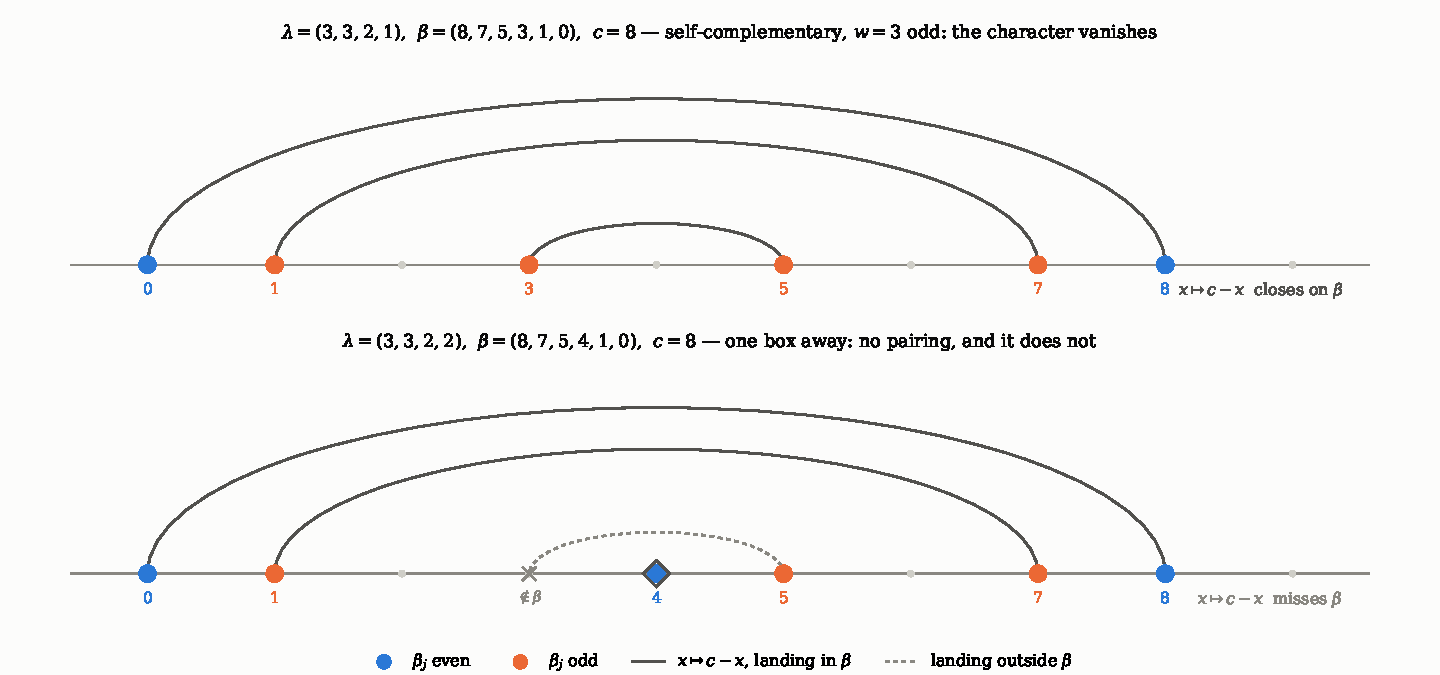
\includegraphics[width=\textwidth]{fig_involution.pdf}
\caption{Why self-complementarity kills the character. Expanding along the two frozen rows leaves
terms indexed by pairs $(e,o)$ with $e\in E$, $o\in O$, and the reflection $x\mapsto c-x$ acts on
them. Above, a self-complementary shape of odd width: every arc lands in $\beta$ and joins entries of
equal parity, because $c$ is even. Below, the same shape with one box moved: the arc $5\mapsto3$
leaves $\beta$, so there is no pairing and nothing cancels. The diamond marks the fixed point of the
reflection, which cannot occur inside an opposite-parity pair --- which is why the involution is
free.}
\label{fig:involution}
\end{figure}

\begin{proof}[Proof of Theorem \ref{thm:r1}]
Put $c_\ast=z+\bar z$ and let $S_n$ be defined by $S_0=0$, $S_1=1$,
$S_{n+1}=c_\ast S_n-S_{n-1}$, so $\deg_{c_\ast}S_n=n-1$ and $S_{-n}=-S_n$; the value $S_{-1}=-1$ is
used whenever $\beta_N=0$. Since $\Phi_A=(x^2-1)(x^2-c_\ast x+1)$, a polynomial $P$ supported on
$\beta$ is divisible by $\Phi_A$ exactly when $P(1)=P(-1)=0$ and $P\equiv0$ modulo $x^2-c_\ast x+1$.
Splitting $P(\pm1)$ by parity and reducing $x^n\equiv S_nx-S_{n-1}$, admissibility becomes the
singularity of the $4\times4$ matrix with rows $[\beta_j\ \mathrm{even}]$,
$[\beta_j\ \mathrm{odd}]$, $S_{\beta_j}$, $S_{\beta_j-1}$. Expanding along the two parity rows and
using d'Ocagne's identity \cite{Doc} for this recurrence,
\begin{equation}\label{eq:docagne}
S_bS_{b'-1}-S_{b'}S_{b-1}=-S_{b-b'},
\end{equation}
each $2\times2$ block collapses to a \emph{single} $S$, indexed by the difference of the two
surviving $\beta$'s. Distinct $S_n$ have distinct degrees in $c_\ast$ and are therefore linearly
independent, so the signed sum vanishes only by exact pairing of equal indices with opposite signs.
The case analysis is finite: $|E|\in\{0,4\}$ is branch (a); $|E|\in\{1,3\}$ leaves three terms whose
indices are the three pairwise differences of a $3$-set and hence always distinct, so no pairing
exists and the value is nonzero; and for $|E|=2$ there are four terms and three perfect matchings,
and one checks the six parity patterns directly. For $E=\{\beta_1,\beta_4\}$ and for
$E=\{\beta_2,\beta_3\}$ exactly one of the three matchings is available and it imposes the single
condition $\beta_1+\beta_4=\beta_2+\beta_3$, which is branch (b); for the four remaining patterns
every one of the three matchings forces two distinct entries of $\beta$ to coincide, so none is
available and the value is nonzero.
\end{proof}

Identity \eqref{eq:docagne} is classical. The collapse it produces is an accident of rank one: two
letters admit a single gap, so $s_{(m,n)}(z,\bar z)=S_{m-n+1}$ depends on that gap alone. There is no
rank-$r$ analogue. One would be a closed form for $s_\mu$ at a reciprocal alphabet for \emph{every}
$\mu$; \cite{CK09} supply that for rectangular shapes and \cite{AB19} for self-complementary ones,
and nobody in general.

For general $r$ we use associates, in Littlewood's sense \cite{Lit50}. On the $\det=-1$ coset $[\nu^{*}]=[\nu]\otimes\det$ gives
$\Psi_r=\sum_\nu\big(m_\nu-m_{\nu^{*}}\big)\chi_{[\nu]}$, so $\Psi_r=0$ if and only if
$m_\nu(\lambda)=m_{\nu^{*}}(\lambda)$ for every $\nu$; equivalently, $V_\lambda|_{O(N)}$ is
$\det$-invariant. A witness is therefore a single $\nu$ with $m_\nu\ne m_{\nu^{*}}$, and it can be
constructed.

Karmakar's \cite[Theorem 4.1]{Kar24} determines the value at the endpoint $z_i=1$, which is an element
of order two: case (A) is branch (a), case (B) is a nonzero dimension, and case (C) leaves an
alternating sum of products of dimensions with no vanishing criterion attached. Branch (b) lives in
that case (C), so the theorem below is not a consequence of it. Nor does case (B) help more as $r$
grows: at $k=1$ it asks that $N-1$ of the $N$ beta numbers share a parity, and the smallest shape
doing so is the staircase $(2r-1,2r-2,\dots,1)$, of size $r(2r-1)$, so on a fixed range of
$|\lambda|$ his nonvanishing case is visible only for small $r$ --- his result is sharpest exactly
where ours is easiest. What connects the endpoint to the
curve at all is rigidity, and rigidity is a statement about our object rather than about the order-two
element: over the ranges of \S\ref{sec:verif} it holds on $\ell(\lambda)\le N/2$ without exception
and fails outside, which is Remark \ref{rem:rankone}.

\begin{proof}[Proof of Theorem \ref{thm:stable}]
Branch (a) cannot occur: with $\ell(\lambda)\le N/2$ at least two trailing parts vanish, so $\beta$
contains two consecutive integers. In Littlewood's range
$m_\nu(\lambda)=\sum_{\beta'\ \mathrm{even}}c^{\lambda}_{\nu\beta'}$, and the term $\beta'=\emptyset$
gives $m_\mu\ge1$ for every $\mu\subseteq\lambda$. Take $\mu$ as follows. If
$\ell(\lambda)<N/2$, take $\mu=\lambda$: then $\ell(\lambda^{*})=N-\ell(\lambda)>\ell(\lambda)$, so
$\lambda^{*}\not\subseteq\lambda$ and $m_{\lambda^{*}}=0\ne m_\lambda$. If $\ell(\lambda)=N/2$ and
$\lambda_{N/2}$ is even, take $\mu=(\lambda_1,\dots,\lambda_{N/2-1})$; then
$\beta'=(\lambda_{N/2})$ is even, $\lambda/\mu$ is a horizontal strip and $m_\mu\ge1$ while
$\ell(\mu)<N/2$, so the previous computation applies to $\mu$. If $\ell(\lambda)=N/2$ and $\lambda$
is not a rectangle, let $j\le N/2-1$ be largest with $\lambda_j>\lambda_{j+1}$ and remove both the
last row and one box from row $j$; then $\beta'=(\lambda_{N/2}+1)$ is even and
$\lambda_j\ge\lambda_{N/2}+1$ keeps $\lambda/\mu$ a horizontal strip. In the remaining case
$\lambda=(k^{\,N/2})$ neither construction is available, and $k$ odd is branch (b) while $k$ even
falls to the second construction.
\end{proof}

\subsection{Outside Littlewood's range}\label{sec:unstable}

For $\ell(\lambda)>N/2$ the restriction rule acquires non-standard labels, and the modification rules
that reduce them are King's \cite{King71}; Koike and Terada \cite{KT87} record that the
type-$D$ specialization sends a universal character to $0$ or to $\pm$ one other, and Fauser, Jarvis,
King and Wybourne observe that beyond the two classical cases \emph{``the general theory, having
infinitely many cases, needs a not yet available formalism''} \cite[\S4]{FJKW05}. Extensions of Littlewood's rule to all parameters do exist for the two classical
cases --- Newell's modification rules \cite{New51}, Sundaram \cite{Sun90} in the symplectic case,
Gavarini's Brauer-algebra proof \cite{Gav99}, and Enright and Willenbring \cite{EW04}, whose Theorem 4
gives the multiplicity as an alternating sum over the Weyl group which in favourable cases collapses
to a difference of two Littlewood coefficients \cite[\S7.11]{EW04}. The route taken here is the dual
one: keep the coefficients universal, which they are in every range, and move the whole
range-dependence into the values, where one lemma disposes of it. On this alphabet no formalism for
the labels is needed at all, and the reason is that the values are not type-$D$ values.

Adding a letter $c$ to an alphabet acts on the ring of symmetric functions by $p_k\mapsto p_k+c^k$;
write $\iota_c$ for that homomorphism. From the generating function of the complete homogeneous
symmetric functions, $h_m(W,c)-c\,h_{m-1}(W,c)=h_m(W)$ for every $m$.

\begin{lemma}[the alphabet is symplectic]\label{lem:AtoSp}
$\iota_{-1}\iota_{1}\,o_\nu=sp_\nu$ for every partition $\nu$, as an identity between Koike--Terada
\emph{universal} characters in $\Lambda$. In particular, for the alphabet
\eqref{eq:psir},
\begin{equation}\label{eq:AtoSp}
o_\nu(A)\;=\;sp_\nu(z_1,\dots,z_r)
\end{equation}
with no hypothesis on $\ell(\nu)$ and with no sign. For $\ell(\nu)>r$ the right-hand side is
that universal character specialized at $r$ variables, not an irreducible $Sp(2r)$ character; it is
the modification rules below that fold it onto one.
\end{lemma}

\begin{proof}
Both steps are Ayyer and Kumari's, and both are the same manipulation: the recurrence turns the
column operations $C_j\to C_j-c\,C_{j-1}$, applied for $j=n,\dots,2$ in that order, into a change of
character type, and operations of that shape leave a determinant unchanged. At $c=1$ they carry the
defining determinant of $o_\nu$ evaluated at $(W,1)$ to that of the odd orthogonal universal
character $so_\nu$ over $W$, which is Koike and Terada's dictionary in the form
$so_\nu(X)=o_\nu(X,\bar X,1,0,0,\dots)$ \cite[(2.13)]{AK25}. At $c=-1$, where the recurrence is
\cite[Proposition 2.1]{AK25} and the operations read $C_j\to C_j+C_{j-1}$, they carry $so_\nu$ to
$sp_\nu$, which is \cite[Lemma 3.2]{AK25}. Composing gives the first statement, and evaluating it on
the reciprocal alphabet $(z_1,\dots,z_r)$ gives \eqref{eq:AtoSp}.
\end{proof}

\noindent Since $\nu'_1=\ell(\nu)$, the trichotomy on $\nu'_1$ against $N/2=r+1$ is a trichotomy on
the length of $\nu$ against the rank of $Sp(2r)$, and the three facts we need are then the classical
symplectic modification rules --- one of the two cases \cite{FJKW05} exempts --- read through
\eqref{eq:AtoSp}: $o_\nu(A)=0$ when $\ell(\nu)=r+1$, the vanishing of a symplectic character one row
past its rank; $o_\nu(A)=\pm o_{\nu^{*}}(A)$ when $\ell(\nu)>r+1$, King's rule folding the label back
onto a dominant one; and the same for non-standard $\nu$, which by Lemma \ref{lem:nonstd} are exactly
the tall ones. The expansion $s_\lambda=\sum_\nu c_\nu o_\nu$, with
$c_\nu=\sum_{\beta'\ \mathrm{even}}c^{\lambda}_{\nu\beta'}$, is an identity of symmetric functions and
holds in every range; specializing it at \eqref{eq:psir} therefore lands every term on
$\{o_\mu(A):\ell(\mu)\le r\}$, which by \eqref{eq:AtoSp} is the set of irreducible characters of
$Sp(2r)$ and so is linearly independent. Figure \ref{fig:reduction} sorts the labels into the four
classes this paragraph describes and computes $o_\nu(A)$ on each, so that the reduction can be seen
to land where it is claimed to. Hence

\begin{figure}[!ht]
\centering
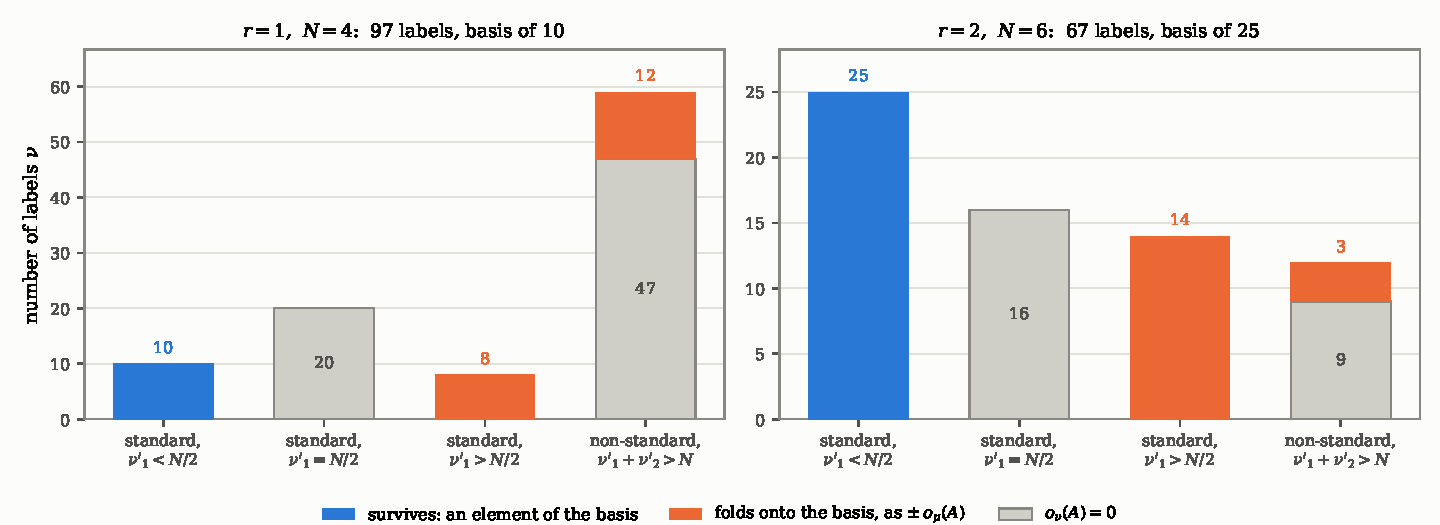
\includegraphics[width=\textwidth]{fig_reduction.pdf}
\caption{The reduction of Lemma \ref{lem:AtoSp}, drawn. Each label $\nu$
occurring in $s_\lambda=\sum_\nu c_\nu o_\nu$ is placed in one of four classes and its value
$o_\nu(A)$ computed. Self-associate labels vanish, every one of them; labels standard with
$\nu'_1>N/2$ fold onto the basis as $\pm o_{\mu}(A)$; non-standard labels either vanish or fold onto
a single basis element with coefficient $\pm1$. By \eqref{eq:AtoSp} these three are the symplectic
modification rules in disguise, the classes being cut by $\ell(\nu)$ against the rank $r$; the figure
was computed before that was noticed, and is left as drawn. Everything lands on the independent
basis $\{o_\mu(A):\ell(\mu)\le r\}$, which is what turns the vanishing into the finite condition
\eqref{eq:Cmu}. The bar heights are label counts over the range each panel was computed on, which is
smaller than the range of the corresponding row of \S\ref{sec:verif}; the classification, not the
count, is what the picture is about.}
\label{fig:reduction}
\end{figure}
\begin{equation}\label{eq:Cmu}
\Psi_r(\lambda)=\sum_{\ell(\mu)\le r}C_\mu(\lambda)\,o_\mu(A),
\qquad
\Psi_r(\lambda)=0\iff C_\mu(\lambda)=0\ \text{for all }\mu,
\end{equation}
where $C_\mu=c_\mu\pm c_{\mu^{*}}+\sum\pm c_\nu$ over the non-standard $\nu$ reducing to $\mu$. The
reduction is carried out in two steps rather than one: most non-standard labels pair with an associate
inside the range, while $21$ of them --- $18$ at $r=1$ and $3$ at $r=2$ --- have no associate in range
and are reduced separately, each landing in the span of the standard values with integer coefficients.

We had computed the three facts before locating them, and record the computation because it is what
the figure below draws: \texttt{sec8\_derivation.sage} checks \eqref{eq:AtoSp} directly for all
$|\nu|\le8$, confirms that the labels of length $r+1$ vanish and that longer ones fold onto the basis
with a sign, and verifies the independence as a rank computation, at $r=1,2,3$. A control that had to
fire: $\iota_1 o_\nu$ and $\iota_{-1}o_\nu$ each agree with $sp_\nu$ only for $\nu=\varnothing$, so
both letters are needed and \eqref{eq:AtoSp} is a statement about the reciprocal pair, not about
either letter alone. \texttt{sec8\_formulas.sage} checks the proof rather than the statement --- the
recurrence at four values of $c$, the two defining determinants against an independent
implementation, and the column operations entry by entry. That last check earned its keep: an earlier
draft of the proof wrote $C_j\to C_j+C_{j-1}$ at $c=1$, the sign \cite[Lemma 3.2]{AK25} uses for its
own step at $c=-1$.

The non-standard labels, which are the whole obstruction here, cannot be small:

\begin{lemma}[non-standard labels are large]\label{lem:nonstd}
Every non-standard $\nu$ occurring in the expansion satisfies $|\nu|\ge N+1=2r+3$. Consequently, if
$|\lambda|\le2r+2$ then no non-standard label is contained in $\lambda$, the last sum in $C_\mu$ is
empty, and $C_\mu(\lambda)=c_\mu(\lambda)\pm c_{\mu^{*}}(\lambda)$ --- with no hypothesis on
$\ell(\lambda)$, hence also outside Littlewood's range.
\end{lemma}

\begin{proof}
Since $c^{\lambda}_{\nu\beta'}=0$ unless $\nu\subseteq\lambda$, only labels with
$\ell(\nu)\le\ell(\lambda)\le N$ occur. Non-standard means $\nu'_1+\nu'_2>N$. Were $\nu$ a single
column we would have $\nu'_2=0$ and hence $\nu'_1=\ell(\nu)>N$, which is excluded; so $\nu'_2\ge1$ and
$|\nu|\ge\nu'_1+\nu'_2>N=2r+2$. A non-standard $\nu$ can therefore contribute only when
$|\lambda|\ge|\nu|\ge2r+3$.
\end{proof}

\noindent Since $\ell(\lambda)>N/2$ forces $|\lambda|\ge r+2$, Lemma \ref{lem:nonstd} settles the
band $r+2\le|\lambda|\le2r+2$ of the unstable range outright: there Littlewood's rule applies
verbatim and the converse follows by the argument of Theorem \ref{thm:stable}. What is left open is
$|\lambda|>2r+2$.


Two exact facts bound the competitors. First $\ell(\mu^{*})=N-\ell(\mu)$, so $\ell(\mu)\le
N-1-\ell(\lambda)$ forces $\mu^{*}\not\subseteq\lambda$ and $c_{\mu^{*}}=0$. Second, a non-standard
$\nu$ has $\nu'_1+\nu'_2>N$ with $\nu'_2\le\nu'_1$, hence $2\ell(\nu)>N$ and $\ell(\nu)\ge r+2$; in
particular no non-standard label fits inside $\lambda$ in Littlewood's range. Call $\mu$
\emph{isolating} for $\lambda$ if exactly one of the labels feeding $C_\mu$ is contained in
$\lambda$; then $C_\mu=\pm c_\nu\ne0$ and $\Psi_r(\lambda)\ne0$. What remains open is one existence
statement.

\begin{proposition}[the isolating witness does not always exist]\label{conj:iso}
At $r=2$ the shape $\lambda=(5,5,2,1)$ has $\Psi_2(\lambda)\ne0$ and is of neither type {\rm(a)} nor
type {\rm(b)}, and no $\mu$ is isolating for it: every $\mu$ whose $C_\mu$ has a nonzero contributor
inside $\lambda$ has exactly two, namely $\mu$ and its associate $\mu^{*}$.
\end{proposition}

We had proposed the isolating witness as the route to Conjecture \ref{conj:crit}, and it does not
reach. The reason is legible in the isolation lemma: it needs $\ell(\mu)\le N-1-\ell(\lambda)$, which
at $\ell(\lambda)=4$ and $N=6$ leaves only one-row $\mu$, and a shape as wide as $(5,5,2,1)$ contains
every associate. Over $r=2$ and $|\lambda|\le14$ there are eleven such shapes, and none at all below
$|\lambda|=13$, which is why the certificate looks sound on small ranges. Conjecture \ref{conj:crit}
itself is untouched --- it asserts that the $C_\mu$ vanish, not that a certificate exists, and it
holds over every shape in the ranges of \S\ref{sec:verif} --- but it is left without a route.

The mechanism does reach a great deal: at $r=2$ and $|\lambda|\le14$, $227$ of the $238$ non-vanishing
unstable shapes carry a proved isolating witness. It also reaches further than fact (ii) allows on
its own --- the true minimum of $\ell(\nu)$ over non-standard $\nu$ with $o_\nu(A)\ne0$ is $5$ there,
against the $r+2=4$ the bound gives. What defeats it is width rather than height: the basis in
\eqref{eq:Cmu} grows with $r$ and the competing labels are constrained to be tall, so we had read
isolation as getting easier with $r$, and along the height axis it does; the residue lives where
$\lambda$ is wide enough to swallow the associates. That reading predicts where the residue is
\emph{not}: at $r=3$ the isolation lemma allows $\ell(\mu)\le7-\ell(\lambda)$, so a shape must be
wider than at $r=2$ before it can swallow every associate, and the same sizes should come out clean.
They do --- over $r=3$ and $|\lambda|\le13$ all $149$ non-vanishing unstable shapes carry a proved
witness and the residue is empty --- which is a control on the explanation rather than a step toward
the conjecture. At $r=1$ the question does not arise, since that case is settled independently by
Theorem \ref{thm:r1}.

The tool one reaches for first does not fit. Saturation, in the honeycomb form of Knutson and Tao
\cite{KT99}, decides when a single Littlewood--Richardson coefficient is positive, and every
competitor feeding $C_\mu$ is positive as soon as its label sits inside $\lambda$. What an isolating
$\mu$ asks for is not positivity but \emph{isolation}: that exactly one of them does. The positivity
is what makes the question hard rather than what answers it, and we know of no tool aimed at the
second question.

\begin{figure}[tb]
\centering
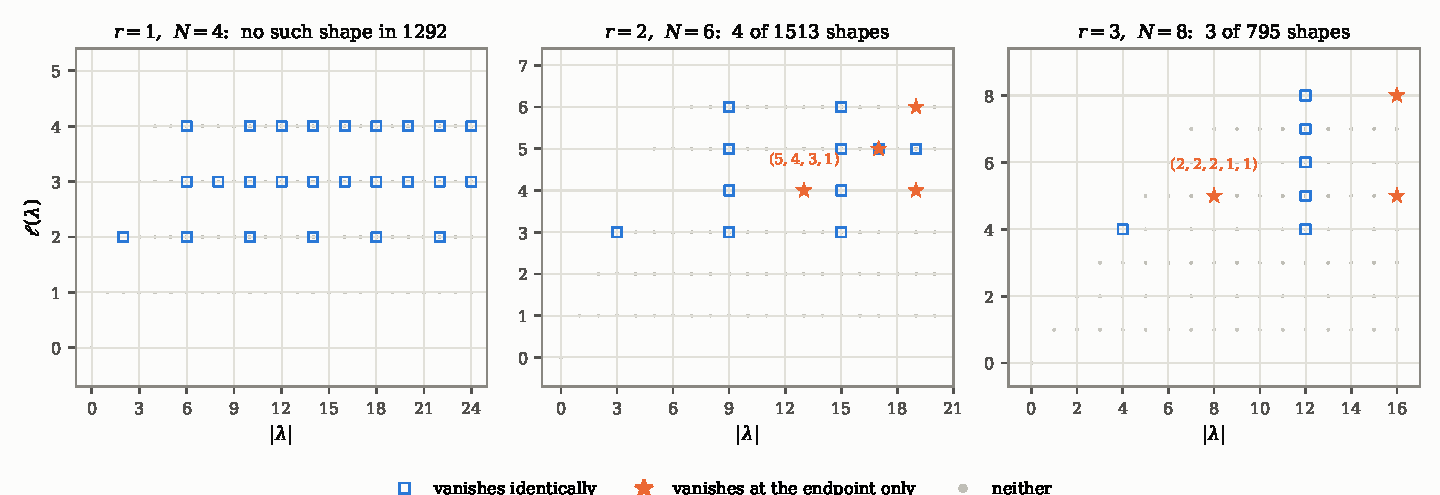
\includegraphics[width=\textwidth]{fig_phase.pdf}
\caption{Where one reciprocal pair stops being typical. Each partition with at most $N$ parts is a
point at $(|\lambda|,\ell(\lambda))$; the class drawn as a star is the one that vanishes at the
endpoint $z_i=1$ without vanishing identically, and it is the whole content of the picture; each
panel names its smallest member and Remark \ref{rem:rankone} lists the rest. The panels cover
$|\lambda|\le24$, $20$ and $16$ respectively. At $r=1$ the class is
empty over all $1292$ shapes in range, because the object there is $\pm$ a genuine character and its
value at the identity is a dimension. From $r=2$ on the object is properly virtual and the class is
not empty. See Remark \ref{rem:rankone}.}
\label{fig:phase}
\end{figure}

\begin{remark}[the rank-one accident, and where the two ranges part]\label{rem:rankone}
At $r=1$ the object is $\pm$ a genuine character, so its value at the identity is a dimension and
$\Psi_1(\lambda)\equiv0$ if and only if $\Psi_1(\lambda)|_{z=1}=0$. At $r\ge2$ the object is properly
virtual and that equivalence fails: $\lambda=(5,4,3,1)$ at $r=2$ has $\Psi_2(\lambda)\ne0$ and
$\Psi_2(\lambda)|_{z_1=z_2=1}=0$. Over the ranges of Figure \ref{fig:phase} the class of such shapes
is empty at $r=1$ across $1292$ partitions; at $r=2$ it consists of the four shapes $(5,4,3,1)$,
$(5,5,4,2,1)$, $(10,5,3,1)$ and $(6,5,4,2,1,1)$, and at $r=3$ of the three shapes $(2,2,2,1,1)$,
$(5,5,4,1,1)$ and $(3,3,3,2,2,1,1,1)$; it is thin, but it is not empty, and one counterexample is all
the equivalence can survive. The surviving implication, exact vanishing $\Rightarrow$ vanishing
at the endpoint, is what makes the endpoint a valid sieve and no more. This is why results computed
at elements of order two \cite{Kar24}, or at variables set to $1$ \cite{Eis07}, bear on the endpoint
and not on the curve, and why Theorem \ref{thm:zeros} is not a corollary of them for $r\ge2$.
\end{remark}

It is worth putting a number on what the endpoint sieve loses, since the qualitative statement is
easy to misread as a small correction. Over the ranges of Figure \ref{fig:phase} the test
$\Psi_r(\lambda)|_{z_i=1}=0$ flags $143$ shapes at $r=1$, $22$ at $r=2$ and $9$ at $r=3$; of those,
$0$, $4$ and $3$ respectively do not vanish identically. So the sieve is exact at one pair, and the
fraction of its verdicts that are spurious grows with the number of pairs --- $0\%$, $18\%$, $33\%$
over these ranges. An endpoint computation is a filter that never misses a genuine zero, and past one
pair it is nothing more than that. The rank-one case at $t=2$, where the sieve happens to be exact
because the object is a genuine character, was treated separately in \cite{Mar26}; the alphabet
\eqref{eq:object} arose there, in a Wilson-line computation on an orbifold, which is why $-1$ appears
as a letter rather than as a choice.

The reason the two ranges of $\ell(\lambda)$ behave so differently is worth separating from the
mechanism that proves it. Littlewood's rule is a statement about which labels $\nu$ can occur, and
$\ell(\lambda)\le N/2$ is exactly the condition under which the non-standard ones cannot fit inside
$\lambda$ at all. Lemma \ref{lem:nonstd} says that the obstruction is governed by $|\lambda|$ as well
as by $\ell(\lambda)$, so the honest picture is not two ranges but a region: the converse is proved
wherever either $\ell(\lambda)\le N/2$ or $|\lambda|\le2r+2$, and outside their union it is open ---
the isolating witness covers most of that region but provably not all of it, by Proposition
\ref{conj:iso}.

%======================================================================
\section{Verification}\label{sec:verif}

Every statement above was checked numerically, by two implementations along different code paths: one
in exact Laurent arithmetic, and one a from-scratch bialternant evaluation written from the
statements alone. The ranges and counts are collected here once.

\begin{center}\footnotesize\setlength{\tabcolsep}{4.2pt}
\begin{tabular}{llrl}
\toprule
statement & range & result & status\\
\midrule
Theorem \ref{thm:main}, sign included & $t\le7$, $|\lambda|\le14,\dots,10$ &
$959$ exact, $476$ zeros, $0$ fail & \stproved\\
Lemma \ref{lem:L1} & $t\le6$ & $454$ nonzero minors & \stproved\\
Lemma \ref{lem:L4} & $t\le7$ & $724/724$ & \stproved\\
Proposition \ref{prop:quotient} & $t\le7$, $|\lambda|\le19$ & $2970/2970$ & \stproved\\
Proposition \ref{rem:lattice} (the concentric locus) & $t\le9$, $|\lambda|\le16$ & $1331/1331$;
$0$ at odd $t$, $43$ at even & \stproved\\
Proposition \ref{rem:sign} (short form of the sign) & $t\le8$, $|\lambda|\le14$ & $1496/1496$;
proof steps $0$ fail & \stproved\\
Proposition \ref{prop:fibrelattice} (the lattice) & $t\le5$, $|\lambda|\le14,12,10,10$ &
$84$, $35$, $20$, $14$ fibres, both ways & \stproved\\
Corollary \ref{cor:fibregf} (the generating function) & same range &
$153/153$; wrong denominator $101$ & \stproved\\
Remark \ref{rem:signsees} (the sign sees the $m_i$) & $t\le4$ &
$107/107$, $43/62$, $26/36$ & \stverif\\
Lemma \ref{lem:single} & $t\le7$, $|\lambda|\le16$ & $2113/2113$ & \stproved\\
Theorem \ref{thm:extra} & $t\le12$, $\lambda_1\le33$ & $119+21$, no others & \stproved\\
Proposition \ref{prop:rect} & $t=2$, $r\le4$, $c\le60$ & $240/240$ & \stproved\\
Corollary \ref{cor:enum} against direct enumeration & $t\le5$ & $14/14$; boxes $16/16$ &
\stproved\\
Proposition \ref{rem:involution} (the runs alternate) & $t=2$, $|\lambda|\le14$, $\le4$ rows &
$4823$ minors; $217$ pairs, $0$ fail & \stproved\\
(D3), (D4) of \S\ref{sec:sharp} & $t\le6$, $|\lambda|\le10$ &
$600$ / $383$ / $200$ of $600$ & \stverif\\
\midrule
\rowcolor{hband} Theorem \ref{thm:zeros}, both directions & $r\le3$, $|\lambda|\le28,26,22$ &
$9961$ shapes, $318$ zeros, $0$ fail & \stverif\\
\rowcolor{hband} \quad branch (a), Thm.~\ref{thm:zeros} & $r\le3$, $|\lambda|\le15$ &
$16/16$ & \stproved\\
\rowcolor{hband} \quad branch (b), Thm.~\ref{thm:zeros} & $r\le3$ & $24/24$ & \stproved\\
\rowcolor{hband} \quad even-width control for (b) & $r\le3$ & $56/56$ nonzero & \stproved\\
\rowcolor{hband} \quad converse at $r=1$, Thm.~\ref{thm:r1} & $\beta_1\le25$ &
$14950$ beta sets, $0$ fail & \stproved\\
\rowcolor{hband} \quad converse, $\ell(\lambda)\le N/2$, Thm.~\ref{thm:stable} & $r\le3$ &
$372/372$ witnesses & \stproved\\
\rowcolor{hband} \quad the isolating witness, Prop.~\ref{conj:iso} & $r=2$, $|\lambda|\le14$ &
$227$ witnesses, $11$ residue & \stproved\\
\rowcolor{hband} \quad the same at $r=3$ & $r=3$, $|\lambda|\le13$ &
$149$ witnesses, $0$ residue & \stproved\\
\midrule
Identity \eqref{eq:compl} & $r\le2$ & $474/474$ & \stproved\\
Identity \eqref{eq:docagne}, and $\deg_{c_\ast}S_n=n-1$ & $b\le31$ & $496/496$; $39/39$ &
\stproved\\
Lemma \ref{lem:AtoSp}, the \S\ref{sec:unstable} reduction & $r\le3$, $|\nu|\le8$ &
identity $0$ fail; folds $0$ fail & \stproved\\
\quad the reduction carried out & $r\le2$ & $236$ labels, $0$ unresolved & \stproved\\
\eqref{eq:Cmu} against the exact object & $r\le2$, both ranges & $184$ shapes, $0$ fail &
\stverif\\
\bottomrule
\end{tabular}
\end{center}

\noindent The shaded block is Theorem \ref{thm:zeros} read from the top down: the two sufficient
branches are proved for every $r$, the converse is proved for one pair and, for every $r$, inside
Littlewood's range, and one line remains --- the converse for $r\ge2$ outside that range and beyond
the band $|\lambda|\le2r+2$ that Lemma \ref{lem:nonstd} settles, which is Conjecture
\ref{conj:crit}. That single \stverif\ line is why the first row of the block is not
labelled \stproved. The row below it records what the certificate we proposed for that line does and
does not do, and it is labelled \stproved\ because Proposition \ref{conj:iso} is a counterexample and
counterexamples are proofs. The rows below the block are the identities and the reduction the section rests
on. In the column, \stproved\ means a proof is given here or cited, and \stverif\ means the
statement is checked exhaustively over the stated range and not proved.

\noindent The (D3), (D4) row is the one that matters most in the first group: the identity holds in
all $600$ cases for \eqref{eq:object} and fails in $217$ and $400$ of them for the two deformed
alphabets, so the test is capable of failing. In the second group the even-width control plays the
same role for Theorem \ref{thm:zeros}: $56$ self-complementary shapes of even width, none of which
vanishes, so the parity hypothesis is doing work rather than decorating. A separate audit rebuilds
all of the second group from the definitions in a single pass, independently of the scripts that
produced them: $3414$ checks, $0$ failures. A second one takes the \emph{displayed formulas} rather
than the counts --- Theorem \ref{thm:LR}, the interval reading \eqref{eq:intervals}, Lemmas
\ref{lem:L2} and \ref{lem:L5}, the splitting \eqref{eq:threestep}, the complementation
\eqref{eq:compl}, d'Ocagne \eqref{eq:docagne} and the scalar caveat \eqref{eq:scalar} --- and
evaluates both sides at numeric points from the definitions, using neither the closed forms of this
paper nor the scripts behind the table: $3297$ evaluations over nine displayed formulas, $0$ failures. The scripts are ancillary to this paper, and so is the
saved output of each one, so every count in the table above can be located in an archived run rather
than taken on trust.

%======================================================================
\section{Open problems}\label{sec:open}

\begin{problem}[the other classical types]\label{prob:types}
Everything above is type $A$. What do $sp_\lambda(\zt,z,\zb)$, $so_\lambda(\zt,z,\zb)$ and
$o_\lambda(\zt,z,\zb)$ do? The root-of-unity factorizations were carried from type $A$ to $B$, $C$,
$D$ by a uniform argument in \cite{AK22} and to the universal characters in \cite{Alb23}; the frozen
rows of the bialternant are the same in every type, so Lemma \ref{lem:L1} and the excess-two count
should survive verbatim, while the collapse, Lemmas \ref{lem:L4} and \ref{lem:L5}, would need
re-deriving once per type. The alphabet \eqref{eq:object} is already a torus element of $O(t+2)$, so
the other types are not the same function at a new point but new objects, and choosing the right ones
is a matter of taste inside a programme we did not build. We have measured, and report it as a
measurement only. Expanding the Koike--Terada universal characters in the Schur basis and evaluating
term by term with Theorem \ref{thm:main}, over $|\lambda|\le12$ for $t\le3$ and $|\lambda|\le10$ for $t=4,5$, the fraction of
$\ell(\lambda)\ge2$ shapes on which the value vanishes is markedly larger for $o_\lambda$ on the
non-identity component than on the identity one --- $83.8\%$ at $t=2$ against $41.8\%$ at $t=3$, and
$58.8\%$ at $t=4$ against $42.1\%$ at $t=5$ --- with $sp_\lambda$ in between and the Schur case
lowest. The effect is real and it tracks the component, which is what one would expect of an
associate cancellation; but it is quantitative and we found no law covering the whole table. A first
attempt at one, that
$o_\lambda$ vanishes for all $\ell(\lambda)\ge2$ when $t$ is even, is false: it was read off a
sample and the systematic sweep refutes it.

The $t=2$ column of that comparison is the one case which does have a law, and it is Lemma
\ref{lem:AtoSp}: there the alphabet is \eqref{eq:psir} at $r=1$, so $o_\nu$ equals $sp_\nu(z)$, a
\emph{rank-one} symplectic character. That vanishes identically for $\ell(\nu)=2$ --- all $36$ such
shapes in range, with no exception --- and folds for $\ell(\nu)>2$, which is why the $t=2$ figure is
the outlier. What remains without a law is odd $t$, where the alphabet is not of the form
\eqref{eq:psir} and the lemma does not apply.

The $sp_\lambda$ column at $t=2$, on the other hand, has an answer, and it explains the asymmetry of
the table rather than adding a row to it. Adjoining the same two letters to a universal
\emph{symplectic} character does not collapse it. Over $|\nu|\le8$,
\begin{equation}\label{eq:spbranch}
sp_\nu(W,1,-1)\;=\;\sum_{\gamma\subseteq\nu}c_{\nu/\gamma}\;sp_\gamma(W),
\end{equation}
where the coefficient depends on $\nu$ and $\gamma$ only through the skew shape $\nu/\gamma$ ---
$247$ coefficients over $74$ distinct skew shapes, with no clash --- and takes only the values $0$
and $\pm1$, vanishing whenever $|\nu/\gamma|$ is odd. That is the shape a branching rule for
universal symplectic functions produces, and such rules are available \cite{JJLW24}. Read against it,
Lemma \ref{lem:AtoSp} says that for $o_\nu$ the corresponding coefficients are concentrated at
$\gamma=\nu$: the two letters collapse the orthogonal character to a single symplectic one, and leave
the symplectic character spread over the whole interval below $\nu$. The asymmetry of the measurement
is that, and not an artefact of the ranges. What we have not done is identify $c_{\nu/\gamma}$, which
\eqref{eq:spbranch} makes a question about skew universal symplectic characters at $(1,-1)$ and
nothing more.

The third column resists the same route, and for a structural reason rather than an accidental one.
What answers the other two is that adjoining a letter is the ring map $p_k\mapsto p_k+c^k$, so
$\iota_{1}$ and $\iota_{-1}$ act on $\Lambda$ and compose. The identity that would bring $so$ into
the picture, $so_\nu(X)=o_\nu(X,\bar X,1,0,\dots)$ of \cite[(2.13)]{AK25}, relates the two on a
\emph{doubled} alphabet instead, and a doubling is not an adjunction: the $\iota$'s do not reach it.
So the $so$ column is not a gap of effort but of mechanism, and we leave it stated as such.
\end{problem}

\begin{problem}[a Verschiebung that sees a reciprocal pair]\label{prob:versch}
The operator $\varphi_t$ has nothing to say about a letter outside a $\zeta$-orbit, which is the
structural reason Theorem \ref{thm:main} is not a corollary of anything in that line, and the reason
our proof descends to the alternant. Is there an operator on universal characters, or a
factorization of $\varphi_t$ through a larger algebra, acting on alphabets of the form (union of
$\zeta$-orbits) $\cup$ (reciprocal pairs)? By \S\ref{sec:sharp} such an operator would decide (D1)
and (D2) at once. The discussion there suggests a quantitative form.

What makes the question well posed rather than vague is that each half already has a formalism, and
they are not the same one. The $\zeta$-orbits are the province of $\varphi_t$, in Albion's
formulation \cite{Alb23}. Alphabets closed under inversion are the province of the universal
symplectic and orthogonal functions, which have vertex operator realizations from which their
branching rules follow \cite{JJLW24}. Our alphabet is one of each, and Lemma \ref{lem:AtoSp} is the
one place where the two meet: there the $\zeta$-orbit is $\{1,-1\}$, small enough that adjoining it
is a pair of letter maps rather than an operator. We know of nothing that acts on both halves at
once, and the question is whether the two formalisms compose.
\end{problem}

\begin{proposition}[the rank is the wrong invariant]\label{conj:rank}
Let $A=\zt\cup B$ with $B$ closed under inversion and disjoint from $\zt$, and let $\rho(B)$ be the
rank of the subgroup of $\CC^{\times}$ generated by $B$. Then $\rho(B)=1$ does not imply that
$s_\lambda(A)$ is a product of characters. At $t=2$ and $B=\{z,z^{-1},z^{2},z^{-2}\}$, which has
$\rho(B)=1$, the value at $\lambda=(2)$ has a root off the unit circle, and so has no such
factorization; the same happens for $B=\{z,z^{-1},z^{3},z^{-3}\}$.
\end{proposition}

\begin{proof}
A product of characters $\chi_k(z)=(z^{k+1}-z^{-k-1})/(z-z^{-1})$ has all of its roots on the unit
circle. For $B=\{z,z^{-1},z^{2},z^{-2}\}$ and $\lambda=(2)$ the value is
$z^{-4}+z^{-3}+z^{-2}+z^{-1}+3+z+z^{2}+z^{3}+z^{4}$, whose roots miss the circle by $0.32$; over
$|\lambda|\le8$ this happens for $17$ of the $62$ nonvanishing shapes, and for
$B=\{z,z^{-1},z^{3},z^{-3}\}$ for $18$. On the same range $B=\{z,z^{-1}\}$ has every root on the
circle without exception, as Theorem \ref{thm:main} requires.
\end{proof}

What the rank does not see is how many free directions $B$ has. A single reciprocal pair is one
direction; $\{z,z^{-1},z^{2},z^{-2}\}$ generates a group of rank one and is two, and the two see each
other. So the invariant to conjecture on is not $\rho(B)$ but the number of independent letters,
and with that reading the statement becomes the one \S\ref{sec:sharp} already makes by other means:

\begin{conjecture}[one free direction]\label{conj:rank2}
$s_\lambda(\zt\cup B)$ is a product of characters for every $\lambda$ if and only if $B$ is a single
reciprocal pair.
\end{conjecture}

The evidence for it is Theorem \ref{thm:main} in one direction and (D1)--(D4) together with
Proposition \ref{conj:rank} in the other: enlarging $B$ destroys the product whether the enlargement
raises the rank or not. We have no proof and no proposed mechanism, and this is precisely the
statement a $\varphi_t$-style argument ought to produce.

One caveat, which the conjecture as stated does not cover. Inversion-closure of $B$ is sufficient in
the evidence above, but it is not necessary for a product. Write $w=-iy$. Then the second block of
the alphabet $\{1,-1,y,-y^{-1}\}$ is not closed under inversion, yet
\begin{equation}\label{eq:scalar}
s_\lambda\big(1,-1,y,-y^{-1}\big)\;=\;i^{\,|\lambda|}\,s_\lambda\big(-i,\,i,\,w,\,w^{-1}\big),
\end{equation}
and the alphabet on the right is. The honest hypothesis is therefore that $A$ be a scalar multiple of
an inversion-closed set. A coset $\zeta\zt$ is itself inversion-closed exactly when
$\zeta^{2}=\pm1$, which is where (D3) does and does not break.

\begin{problem}[the instrument for the second pair]\label{prob:instrument}
Section \ref{sec:zeros} reduces the vanishing at $r\ge2$ to a statement about the coefficients
$C_\mu$ of \eqref{eq:Cmu}, which are signed sums of Littlewood coefficients, and Conjecture
\ref{conj:crit} is what remains --- with no certificate for it, since the one we proposed fails by
Proposition \ref{conj:iso}. Lemma \ref{lem:AtoSp} settles the other half of the reduction --- what
the values $o_\nu(A)$ are --- and settles it symplectically: the two readings of the alphabet agree
because they are the same reading, the orbit Lie algebra of $D_{r+1}$ being $C_r$ rather than the
fixed subalgebra $B_r$. What it does not touch is the coefficients. Kumari and Stokke \cite{KS26}
have given Murnaghan--Nakayama rules for symplectic, orthogonal and orthosymplectic Schur functions;
by Lemma \ref{lem:AtoSp} the relevant one here is the symplectic \cite[Theorem 3.4]{KS26}, not the
even orthogonal \cite[Theorem 3.10]{KS26}. Does the recursion it provides compute $C_\mu$? Their rule
carries a third sum beyond the adding and removing of border strips, and it is the one they single out
as complicated; \cite[Corollary 3.5]{KS26} shows it drops out once $\mu_n+1\ge r$, so it is a
shallow-shape phenomenon. An earlier form of this problem asked whether that sum is what accounts for
the failure of Littlewood's rule outside its range; Lemma \ref{lem:AtoSp} answers that it is not,
since the failure is carried by the symplectic modification rules, which act on the labels and not
inside the recursion. The coefficients are what is left, and whether that recursion computes them is
what we have not attempted.
\end{problem}

\begin{problem}[the extra locus, in general]\label{prob:extralocus}
Does Theorem \ref{thm:extra} have an analogue for $sp$, $so$ and $o$? More generally, for which
specializations of the free variables does the criterion \eqref{eq:AK53} acquire extra solutions, and
can the extra locus always be read off the kernel of the specialization acting on the span of the
universal characters, as Remark \ref{rem:why} suggests? If each type acquires a family indexed by an
order-two element of the residue lattice, the principle is real.

The question needs the free part pinned down, and for a computed reason: the extra family is a
phenomenon of the \emph{minimal} alphabet. Adjoin a second reciprocal pair and it is gone --- over
$t=3,4,5,6$ and $|\lambda|\le14$ the locus is then exactly the $t$-cores, for type $s$ no less than
for $sp$ and $o$, while at one pair type $s$ has the two extras of Theorem \ref{thm:extra} at $t=4$
and one at $t=6$. (We test the second pair at $z_2=z_1^{2}$, a specialization, which can only create
coincidences and not remove them, so a count of zero there is a count of zero.) An analogue for
another type must therefore be sought at \emph{that type's} minimal free part, one letter of each
kind; comparing types across free parts of different sizes measures the free part instead, which is
what our first attempt did.

The kernel is the right thing to look at, but its \emph{presence} does not settle the locus; its
size does. Two free parts of the same size can both collapse the independence and behave quite
differently. On the reciprocal locus $s_\mu(z,\zb)=\chi_{\mu_1-\mu_2}(z)$ retains one grading, and
the extra locus is the single family of Theorem \ref{thm:extra}. Replace the pair by the
$\zeta_2$-orbit $(z,-z)$, where $s_\mu(z,-z)=z^{|\mu|}s_\mu(1,-1)$ retains only $|\mu|$ and a sign,
and over $\ell(\lambda)\le2$ the criterion acquires $28$ further solutions at $t=2$ and $186$ at
$t=8$, in no family we can name. The control is the free pair $(z,w)$, which has no kernel and
returns the $t$-cores and nothing else at every $t\le8$ --- that is \eqref{eq:AK53} itself, so the
control is their theorem rather than a measurement of ours. So the
reciprocal pair is the collapsing specialization of \emph{smallest} kernel, and that, rather than
the mere existence of a kernel, is what makes its extra locus one family.
\end{problem}

\begin{problem}[the fibres, refined by the sign]\label{prob:fibres}
Corollary \ref{cor:fibregf} describes the fibre of the interval triple, and only that. The invariant
is $I_t=(d_1,d_2,d_3,\varepsilon_\lambda)$, and the sign cuts each branch further. Its cut is not
bookkeeping, and it is not idle: by Remark \ref{rem:signsees} the sign sees the $t-2$ directions the
triple does not, from $t=3$ on --- constant in $(m_i)$ at fixed $v$ in all $107$ slots at $t=2$, but
in only $43$ of $62$ at $t=3$ and $26$ of $36$ at $t=4$. What is the restriction of
$\varepsilon_\lambda$ to a branch? The obstruction to reading it off \eqref{eq:fibrelattice} is
visible in \eqref{eq:sign}: $\inv(b_S)$ is a statistic of the whole beta-word, and the lattice
coordinates split that word into two distinguished classes and $t-2$ free letters, so a rule would
have to reassemble what the bijection separates.

Two smaller gaps go with it. The same description for the size-three profile should be the same
bookkeeping with one class of three in place of two of two; we have not written it. The degenerate
profile is a different question, since there the fibre is the whole vanishing locus of $\Phi_t$,
which Corollary \ref{cor:zero} and Proposition \ref{rem:lattice} describe by other means.
\end{problem}

\begin{problem}[a sieving phenomenon that keeps a parameter]\label{prob:sieving}
At $t=2$ Corollary \ref{cor:enum} is a signed count of $\mathrm{SSYT}(\lambda,4)$, and a signed count
of order two is what Stembridge's $q=-1$ phenomenon \cite{Ste94} computes: on a set carrying an
involution, the value at $-1$ counts the fixed points. That is the case $\#C=2$ of the cyclic sieving
phenomenon of Reiner, Stanton and White \cite{RSW04}, whose Theorem 4.3 evaluates the principal
specialization $s_\lambda(1,q,\dots,q^{k-1})$ at a primitive $d$-th root of unity in terms of the
$d$-core and the $d$-quotient of $\lambda$ --- the two invariants that carry Theorem \ref{thm:main}
as well --- and which Lee and Oh \cite{LO22} have since extended to skew shapes. Every evaluation in
that line is at a \emph{number}, as a sieving statement requires: the alphabet there is the geometric
progression $1,q,\dots,q^{k-1}$ specialized at a root of unity, not a plain orbit, and nothing is
left free. Ours is not of that kind --- the reciprocal pair keeps $z$, and \eqref{eq:main} is a
product formula in it. Is there a cyclic action on $\mathrm{SSYT}(\lambda,t+2)$, and a $q$-analogue of
$\Phi_t$, whose value at a $t$-th root of unity counts fixed points refined by $m_{t+1}-m_{t+2}$?
The case $\#C=2$ is where to look first, and there the involution such a statement would need already
exists: \S\ref{sec:enum} assembles it.

The existence half of the question is decidable without exhibiting the action. Alexandersson and
Amini \cite{AA19} give a necessary and sufficient criterion for a cyclic action realizing a given
sieving polynomial to exist: for every $d\mid t$, the value at $\omega^d$ must be
$\sum_{j\mid d}j\,c_j$ with every $c_j$ a nonnegative integer, and the $c_j$ --- the numbers of
orbits of each size --- are then computable by triangularity. Applied to the candidate that the
alphabet itself suggests, $F(q,z)=s_\lambda(1,q,\dots,q^{t-1},z,z^{-1})$, whose $z$-grading is
already the refinement asked for, the criterion is met by almost every graded piece in the ranges we
can reach; but so it is for a deliberately wrong refinement, grading by $m_{t+1}+m_{t+2}$ instead,
which passes at the same rate. At those sizes the criterion does not discriminate, and we report the
attempt as evidence in neither direction.
\end{problem}

One narrower gap is recorded where it arises rather than here, in the same form as the problems
above and with the same meaning --- something we would like to know and have not settled: the
involution of \S\ref{sec:enum} is assembled at $t=2$ and nowhere else, because Proposition
\ref{rem:involution} is a statement about one word and that word is the $t=2$ one. The distinction we
keep throughout is between a \emph{conjecture}, which is a statement we believe and have tested, and
a \emph{problem}, which is not a claim at all.

Taken together the problems say where we think the object stops being ours. The evaluation is
complete and the alphabet is minimal, so what is left is not more of the same: it is whether the two
formalisms that own the two halves of \eqref{eq:object} compose, whether a sieving statement can keep
a variable, and what the coefficients $C_\mu$ do once the certificate we proposed for them is gone.
Of the three, the last is the one the paper needs and the first is the one we would rather see
answered.

\subsection*{Acknowledgements}
This paper exists because Arvind Ayyer asked whether the rank-one case generalizes to arbitrary $t$
with the free variable symbolic. The question was better than the note that prompted it. We thank him
for it, and for the correspondence that followed. Remark \ref{rem:core} exists because Nishu Kumari
asked whether the condition $n_i(\lambda)=0$ could be phrased in terms of the $t$-core; she also
confirmed the reading of \cite[Theorem 5.3]{AK25} in \S\ref{sec:independence}, and it was a pointer
of hers that sent us to \cite[\S3]{AK25}, where Lemma \ref{lem:AtoSp} was waiting; we are grateful
for it. The involution of \S\ref{sec:enum} is assembled from three lemmas of her thesis
\cite{KumariThesis}, and is hers in that sense too.

\subsection*{Code, data and disclosure}
Every computation quoted in this paper is performed by a named script distributed as an ancillary
file, and every number quoted is reproduced by an archived run of one; \S\ref{sec:verif} tabulates
which script answers for which claim. The same scripts and the same archived output are also kept at
\url{https://github.com/karlesmarin/schur-orbit-and-reciprocal-pair}, which is a convenience: the
ancillary files carry everything the paper appeals to. Generative AI (Claude, Anthropic) was used
throughout as a
research assistant --- for literature search, for writing and checking the ancillary code, and on the
prose. The mathematics, and the responsibility for it, are the author's.

%======================================================================
\begin{thebibliography}{AAAA}

\bibitem[Alb23]{Alb23} S.~P.~Albion, \emph{Universal characters twisted by roots of unity},
Algebraic Combinatorics; arXiv:2212.07343.

\bibitem[Alb25]{Alb25} S.~P.~Albion, \emph{Character factorisations, $z$-asymmetric partitions and
plethysm}, arXiv:2501.18520.

\bibitem[AA19]{AA19} P.~Alexandersson and N.~Amini, \emph{The cone of cyclic sieving
phenomena}, Discrete Math. \textbf{342} (2019), no.~6, 1581--1601; arXiv:1804.01447.

\bibitem[AB19]{AB19} A.~Ayyer and R.~E.~Behrend, \emph{Factorization theorems for classical group
characters, with applications to alternating sign matrices and plane partitions}, J. Combin. Theory
Ser.~A \textbf{165} (2019), 78--105; arXiv:1804.04514.

\bibitem[AK22]{AK22} A.~Ayyer and N.~Kumari, \emph{Factorization of classical characters twisted by
roots of unity}, J. Algebra \textbf{609} (2022), 437--483; arXiv:2109.11310.

\bibitem[AK25]{AK25} A.~Ayyer and N.~Kumari, \emph{Further results for classical and universal
characters twisted by roots of unity}, J. Algebraic Combin. \textbf{63} (2025), no.~1;
arXiv:2501.00275.

\bibitem[CK09]{CK09} M.~Ciucu and C.~Krattenthaler, \emph{A factorization theorem for classical
group characters, with applications to plane partitions and rhombus tilings}, in: Advances in
Combinatorial Mathematics, Springer, Berlin, 2009.

\bibitem[GKS90]{GKS90} F.~Garvan, D.~Kim and D.~Stanton, \emph{Cranks and $t$-cores},
Invent. Math. \textbf{101} (1990), no.~1, 1--18.

\bibitem[HI24]{HI24} M.~Hidaka and M.~Itoh, \emph{The Schur polynomials in all primitive $n$th roots
of unity}, J. Combin. Theory Ser.~A; arXiv:2403.10817.

\bibitem[Jan73]{Jantzen} J.~C.~Jantzen, \emph{Darstellungen halbeinfacher algebraischer Gruppen},
Bonner Math. Schriften \textbf{67} (1973).

\bibitem[Kar22]{Kar22} C.~Karmakar, \emph{Character factorizations for representations of
$GL(n,\CC)$}, arXiv:2210.03544.

\bibitem[Kar24]{Kar24} C.~Karmakar, \emph{Character values at elements of order two},
arXiv:2412.17324.

\bibitem[Mar26]{Mar26} C.~Mar\'in, \emph{Schur functions at $(1,-1,t,t^{-1})$: a closed form on the
non-identity component of $O(4)$}, preprint, 2026; \texttt{doi:10.5281/zenodo.21463000}.

\bibitem[JJLW24]{JJLW24} Z.~Jin, N.~Jing, Z.~Li and D.~Wang, \emph{Universal symplectic/orthogonal
functions and general branching rules}, arXiv:2209.00767.

\bibitem[KLP09]{KLP} S.~Kumar, G.~Lusztig and D.~Prasad, \emph{Characters of simply-laced
nonconnected groups versus characters of nonsimply-laced connected groups}, Contemp. Math.
\textbf{478} (2009), 99--101; arXiv:math/0701615.

\bibitem[KT99]{KT99} A.~Knutson and T.~Tao, \emph{The honeycomb model of $GL_n(\CC)$ tensor
products I: proof of the saturation conjecture}, J. Amer. Math. Soc. \textbf{12} (1999), no.~4,
1055--1090.

\bibitem[Kum24]{Kum24} N.~Kumari, \emph{Factorization of classical characters twisted by roots of
unity: II}, J. Pure Appl. Algebra \textbf{228} (2024), no.~11, 107714; arXiv:2212.12477.

\bibitem[KumT]{KumariThesis} N.~Kumari, \emph{Characters of classical groups twisted by roots of
unity}, PhD thesis, Indian Institute of Science, Bangalore, 2023.

\bibitem[Lec09]{Lec09} C.~Lecouvey, \emph{Parabolic Kazhdan--Lusztig polynomials, plethysm and
generalized Hall--Littlewood functions for classical types}, European J. Combin. \textbf{30} (2009),
no.~1, 157--191.

\bibitem[LR34]{LR34} D.~E.~Littlewood and A.~R.~Richardson, \emph{Immanants of some special
matrices}, Q. J. Math. \textbf{os-5} (1934), no.~1, 269--282.

\bibitem[LLT97]{LLT97} A.~Lascoux, B.~Leclerc and J.-Y.~Thibon, \emph{Ribbon tableaux,
Hall--Littlewood functions, quantum affine algebras and unipotent varieties}, J. Math. Phys.
\textbf{38} (1997), no.~2, 1041--1068.

\bibitem[LO22]{LO22} S.-Y.~Lee and Y.-T.~Oh, \emph{Skew Schur polynomials and cyclic sieving
phenomenon}, Electron. J. Combin. \textbf{29} (2022), no.~4, Paper 4.6; arXiv:2112.12394.

\bibitem[Mac95]{Mac95} I.~G.~Macdonald, \emph{Symmetric Functions and Hall Polynomials}, second
edition, Oxford University Press, 1995.

\bibitem[RSW04]{RSW04} V.~Reiner, D.~Stanton and D.~White, \emph{The cyclic sieving phenomenon},
J. Combin. Theory Ser. A \textbf{108} (2004), no.~1, 17--50.

\bibitem[Ste94]{Ste94} J.~R.~Stembridge, \emph{On minuscule representations, plane partitions and
involutions in complex Lie groups}, Duke Math. J. \textbf{73} (1994), no.~2, 469--490.

\bibitem[Oka98]{Oka98} S.~Okada, \emph{Applications of minor summation formulas to
rectangular-shaped representations of classical groups}, J. Algebra \textbf{205} (1998), no.~2,
337--367.

\bibitem[Pra16]{Pra16} D.~Prasad, \emph{A character relationship on $GL_n(\CC)$}, Israel J. Math.
\textbf{211} (2016), no.~1, 257--270.

\bibitem[AF20]{AF20} A.~Ayyer and I.~Fischer, \emph{Bijective proofs of skew Schur polynomial
factorizations}, J. Combin. Theory Ser.~A \textbf{174} (2020), 105241; arXiv:1905.05226.

\bibitem[Eis07]{Eis07} T.~Eisenk\"olbl, \emph{A Schur function identity related to the
$(-1)$-enumeration of self-complementary plane partitions}, J. Combin. Theory Ser.~A \textbf{115}
(2008), 199--212; arXiv:math/0602401.

\bibitem[FJKW05]{FJKW05} B.~Fauser, P.~D.~Jarvis, R.~C.~King and B.~G.~Wybourne, \emph{New branching
rules induced by plethysm}, J. Phys. A \textbf{39} (2006), 2611--2655; arXiv:math-ph/0508034.

\bibitem[Gav99]{Gav99} F.~Gavarini, \emph{A Brauer algebra-theoretic proof of Littlewood's
restriction rules}, J. Algebra \textbf{212} (1999), 240--271.

\bibitem[EW04]{EW04} T.~J.~Enright and J.~F.~Willenbring, \emph{Hilbert series, Howe duality and
branching for classical groups}, Ann. of Math. \textbf{159} (2004), 337--375.

\bibitem[New51]{New51} M.~J.~Newell, \emph{Modification rules for the orthogonal and symplectic
groups}, Proc. Roy. Irish Acad. Sect. A \textbf{54} (1951), 153--163.

\bibitem[Sun90]{Sun90} S.~Sundaram, \emph{Tableaux in the representation theory of the classical Lie
groups}, in \emph{Invariant Theory and Tableaux} (Minneapolis, MN, 1988), IMA Vol. Math. Appl.
\textbf{19}, 191--225, Springer-Verlag, New York, 1990.

\bibitem[IOTZ06]{IOTZ06} M.~Ishikawa, S.~Okada, H.~Tagawa and J.~Zeng, \emph{Generalizations of
Cauchy's determinant and Schur's Pfaffian}, Adv. in Appl. Math. \textbf{36} (2006), 251--287.

\bibitem[Kin71]{King71} R.~C.~King, \emph{Modification rules and products of irreducible
representations of the unitary, orthogonal, and symplectic groups}, J. Math. Phys. \textbf{12}
(1971), 1588--1598.

\bibitem[KT87]{KT87} K.~Koike and I.~Terada, \emph{Young-diagrammatic methods for the representation
theory of the classical groups of type $B_n$, $C_n$, $D_n$}, J. Algebra \textbf{107} (1987),
466--511.

\bibitem[Doc]{Doc} For the name and the surrounding family of identities (Cassini, Catalan,
d'Ocagne, Vajda) see e.g.\ M.~Bunder and J.~Tonien, \emph{Cassini, d'Ocagne and Vajda identities for
$n$-step Fibonacci numbers}, arXiv:2201.06269.

\bibitem[KS26]{KS26} N.~Kumari and A.~Stokke, \emph{Murnaghan--Nakayama rules for symplectic,
orthogonal and orthosymplectic Schur functions}, Discrete Math. \textbf{349} (2026), no.~2;
arXiv:2411.11447.

\bibitem[Kup02]{Kup02} G.~Kuperberg, \emph{Symmetry classes of alternating-sign matrices under one
roof}, Ann. of Math. (2) \textbf{156} (2002), 835--866.

\bibitem[Lit50]{Lit50} D.~E.~Littlewood, \emph{The Theory of Group Characters and Matrix
Representations of Groups}, 2nd ed., Oxford University Press, 1950.

\bibitem[SK23]{SK23} V.~Sathish Kumar, \emph{Flagged skew Schur polynomials twisted by roots of
unity}, arXiv:2306.10289.

\bibitem[Sta86]{Sta86} R.~P.~Stanley, \emph{Symmetries of plane partitions}, J. Combin. Theory
Ser.~A \textbf{43} (1986), 103--113.

\end{thebibliography}

\end{document}
"
% Keeping both here, rather than in a second file, is deliberate: a duplicated source diverges in
% silence and no build ever fails.
\ifdefined\LONGABS
Let $\zt=\{1,\zeta,\dots,\zeta^{t-1}\}$ be the full set of $t$-th roots of unity and let
$(z,z^{-1})$ be a free reciprocal pair. We evaluate $s_\lambda(\zt,z,z^{-1})$ for every $t\ge2$ and
every partition $\lambda$, with no hypothesis on the shape of $\lambda$: it is a signed product of
exactly three factors over a fixed denominator, or zero, and all three arguments are read off the
$t$-quotient of $\lambda$. Equivalently, and with no exponential in sight, it is a ratio of
$\mathfrak{sl}_2$ characters: a triple product over the square of one. What the identity exposes is a
structure, and the structure is the part we expect to outlast it: everything this evaluation can see
of $\lambda$ is a residue profile, an interval triple and a sign, and we isolate that datum as an
\emph{evaluation invariant}. The value factors through it, and it is complete --- two partitions of
any sizes that share the invariant share the value --- so an arbitrarily large partition is
compressed to three integers and a sign. The proof is a Laplace
expansion along the $t$ frozen rows of the
bialternant together with one cancellation lemma in the symmetric group, and it delivers the sign,
which is the sorting sign already present in Littlewood's evaluation of $s_\lambda(\zt)$ and which we
also give in closed form in the notation of Ayyer and Kumari. Three
consequences are recorded. First, a vanishing criterion: the character vanishes exactly when some
residue class modulo $t$ is empty, or when two distinguished classes are concentric as intervals ---
and the second case occurs only for $t$ even, so for odd $t$ an empty class is the only way to
vanish. Second, an extension of a recent independence criterion of Ayyer and Kumari: their theorem
determines when a character is independent of the variables it is twisted by, and we show that for
two-row shapes on the reciprocal locus the criterion acquires exactly one extra family, which we classify by its core
and quotient, and we locate the step of their argument that the specialization removes. Third, an
enumerative reading: the
identity is a product formula for a root-of-unity weighted count of semistandard tableaux in which a
parameter is still free, and at $t=2$ this is a $(-1)$-enumeration of plane partitions in a box
refined by that parameter; a sign-reversing proof of it has to carry that parameter, and we supply
the half of the cancellation that crosses the splitting of the alphabet. Finally we show the
factorization is isolated: it fails under each of the
four deformations of the alphabet --- more reciprocal pairs, more orbit variables, the orbit replaced
by a coset, the reciprocal pair replaced by a free pair --- and a single reading of the proof
accounts for all four failures at once.

What survives the first of those deformations is the \emph{zero locus}, and the last section is about
it. Write $\Psi_r=s_\lambda(1,-1,z_1,z_1^{-1},\dots,z_r,z_r^{-1})$. Two conditions make $\Psi_r$
vanish: the beta set of $\lambda$ having constant parity, and $\lambda$ being self-complementary of
odd width. \emph{That} implication we prove for every $r$ and every $\lambda$, and we claim nothing
for it: it is a short corollary of the complementation identity over an index family Ayyer and
Behrend already single out, and at the same alphabet \emph{without} the letter $-1$ their theorems
make those very shapes factorize instead --- the determinant of the alphabet is what decides.
The new content is the \emph{converse}, that nothing else vanishes. We prove it in three regimes: for
one reciprocal pair; for every $r$, inside Littlewood's range; and, for every $r$, whenever
$|\lambda|\le2r+2$, which reaches outside that range, because a non-standard label cannot be smaller
than that. What is left over remains a \emph{conjecture}; we do not prove it there, and we record
instead that it holds without exception over every shape in the ranges tabulated in the paper. One pair also turns out not to be typical:
there $\Psi_1$ is a genuine character up to sign, so a single order-two specialization decides
whether it vanishes, and from two pairs on that stops being true.
\else
Let $\zt$ be the full set of $t$-th roots of unity and $(z,z^{-1})$ a free reciprocal pair. We
determine how much of a partition $s_\lambda(\zt,z,z^{-1})$ can see: a multiset of three integers
and a sign, and nothing else, so partitions of any sizes agreeing on it share the value. The
evaluation, for every $t\ge2$ and every $\lambda$ with no hypothesis on its shape, is a signed
product of exactly three factors over a fixed denominator, or zero, the three arguments read off
the $t$-quotient. The
proof is a Laplace expansion along the $t$ frozen rows of the bialternant with one cancellation lemma
in the symmetric group, and delivers the sign, the one already in Littlewood's evaluation at
$\zt$.

Three consequences follow. A vanishing criterion: it vanishes exactly when a residue class
modulo $t$ is empty, or two distinguished classes are concentric as intervals, the second only for
$t$ even. An extension of a recent independence criterion of Ayyer-Kumari: for two-row
shapes on the reciprocal locus it acquires exactly one further family, classified by core and quotient. And an
enumerative reading: at $t=2$ a $(-1)$-enumeration of plane partitions in a box refined by a
parameter that stays free. The factorization is isolated: it fails under each of four
deformations of the alphabet, for one reason.

A last section treats the zero locus, which survives further pairs. Two conditions make
$\Psi_r=s_\lambda(1,-1,z_1^{\pm1},\dots,z_r^{\pm1})$ vanish: the beta set having constant parity, and
$\lambda$ being self-complementary of odd width. That direction is a corollary of the complementation
identity over an index family Ayyer and Behrend single out. The new content is the converse, that
nothing else vanishes, proved for one pair, for every $r$ inside Littlewood's range, and for every
$r$ when $|\lambda|\le2r+2$. The rest is conjectural, verified over every shape in the tabulated
ranges.
\fi
\end{abstract}

\maketitle

%======================================================================
\section{Introduction}

A partition can be arbitrarily large, and an alphabet of $N=t+2$ letters can only see so much
of it. This paper settles, for one alphabet, exactly how much. The full set of $t$-th roots of
unity together with one free reciprocal pair sees a multiset of three integers and a sign, and
nothing else whatever: two partitions of any sizes that agree on that datum take the same value
there. The closed form of Theorem \ref{thm:main} is how we prove it, and the compression is the
part we expect to outlast the formula.

The evaluation of Schur polynomials at roots of unity is classical and remarkably clean. Littlewood
and Richardson \cite{LR34} showed that $s_\lambda$ specializes to $0$ or $\pm1$ when the variables
are taken to be all the $t$-th roots of unity, the sign being a sorting sign and the vanishing being
governed by the $t$-core of $\lambda$; and in the same work they generalized this to an alphabet
carrying a free variable in every letter. The latter result was rediscovered by Prasad \cite{Pra16},
given a new proof by Karmakar \cite{Kar22}, extended to all classical groups by Ayyer and Kumari
\cite{AK22} --- who also identified the earlier, almost unnoticed work of Lecouvey \cite{Lec09} ---
and carried to the universal characters by Albion \cite{Alb23}. Kumari \cite{Kum24} extended the
family further, Karmakar \cite{Kar24} treated elements of order two, and Ayyer and Kumari
\cite{AK25} added several more specializations, and Albion \cite{Alb25} related the factorizations to
$z$-asymmetric partitions and plethysm. Sathish Kumar \cite{SK23} carried the factorization to
flagged skew shapes, where it produces a family of Demazure characters; the flags there are
required to be multiples of $t$, which is the same demand for root-of-unity structure in another
guise. We refer to Albion \cite{Alb23} for an account of the whole
line.

A second line of factorization results concerns alphabets closed under $x\mapsto x^{-1}$. Okada
\cite{Oka98} and Ciucu--Krattenthaler \cite{CK09} treated rectangular shapes; Behrend, Fischer and
Konvalinka, and Ayyer, Behrend and Fischer, treated double staircases, for which we follow the
attributions given in \cite{AB19}; and Ayyer--Behrend
\cite{AB19} treated self-dual shapes, with bijective proofs of the latter given by Ayyer and Fischer
\cite{AF20}. There the payoff is enumerative: the factorizations produce
product formulas for symmetry classes of plane partitions and for rhombus tilings. The
self-complementary shapes of \cite{AB19} reappear in \S\ref{sec:zeros} from the other side: adding
the letter $-1$ turns the determinant of the alphabet from $+1$ to $-1$, and the shapes that
factorize there are exactly the shapes that vanish here.

The two lines have never shared an alphabet, and the obstruction is structural in both directions.
The engine of the first is an operator --- the Verschiebung $\varphi_t$, in Albion's formulation
\cite{Alb23}, acting on universal characters by $\varphi_t h_r=h_{r/t}$ if $t\mid r$ and $0$
otherwise --- which requires the alphabet to be a union of $\zeta$-orbits; every extension in that
line therefore adds \emph{more} root-of-unity structure, never less. The engine of the second
requires the alphabet to be entirely reciprocal, or the shape to be self-complementary. A free
reciprocal pair is not a $\zeta$-orbit, and a root-of-unity orbit is not a union of free pairs.

The word \emph{smallest} below can be made precise, and inversion-closure is what makes it so. An
inversion-closed extension of $\zt$ can adjoin only reciprocal pairs $\{x,x^{-1}\}$ and the fixed
points of inversion, which are $1$ and $-1$; and $1$ lies in $\zt$ for every $t$, while $-1$ lies in
$\zt$ exactly when $t$ is even. The only extension smaller than a pair is therefore $\zt\cup\{-1\}$
with $t$ odd, and it is frozen: over $t=3,5,7$ and $|\lambda|\le14$, all $1092$ shapes,
$s_\lambda(\zt,-1)$ takes only the values $0$ and $\pm1$, with nothing left to depend on. A free
reciprocal pair is the smallest extension that leaves anything to evaluate.

In this paper we take the smallest alphabet containing one letter of each kind,
\begin{equation}\label{eq:object}
\Phi_t(\lambda;z)\;:=\;s_\lambda\bigl(\,\underbrace{1,\zeta,\dots,\zeta^{t-1}}_{\zt},\;z,\;z^{-1}\bigr),
\qquad \zeta=e^{2\pi i/t},
\end{equation}
a Schur polynomial in $N=t+2$ variables.

Described that way \eqref{eq:object} is a compromise between two lines, which is how we found it. It
is better described as one object, and that description is what returns in every section below:
\eqref{eq:object} is \emph{a torus element of $O(N)$ with a single free direction}. It is closed
under inversion, so it already lives where the second line lives; its determinant is $(-1)^{t+1}$,
and that determinant is what separates factorizing from vanishing in \S\ref{sec:zeros}; the
$\zeta$-orbit is what places it in the non-identity component when $t$ is even, where a character is
a twining character, which is Remark \ref{rem:twining}; and the one free pair is the one variable
that survives the signed enumeration of \S\ref{sec:enum}. The three results of this paper are three
readings of that sentence.

Our main result, Theorem \ref{thm:main}, evaluates it for
every $t$ and every $\lambda$. Write $\beta=\beta(\lambda,N)$ for the shifted partition and let
$n_i(\lambda)$ be the number of parts of $\beta$ congruent to $i$ modulo $t$, as in \cite{AK22}. Since
there are $t$ residue classes and $N=t+2$ parts, the excess is exactly two, and only three profiles
occur: some $n_i$ vanishes, or two classes have size two, or one class has size three. In the first
case $\Phi_t=0$; in the other two, if $A=\{a_1>a_2\}$ and $B=\{b_1>b_2\}$ denote the two
distinguished classes and
\[
d_1=a_1-a_2,\qquad d_2=b_1-b_2,\qquad d_3=|a_1+a_2-b_1-b_2|,
\]
then, with $z=e^{\theta}$,
\[
\boxed{\;\;\Phi_t(\lambda;z)\;=\;\varepsilon_\lambda\,
\frac{\sinh(d_1\theta/2)\,\sinh(d_2\theta/2)\,\sinh(d_3\theta/2)}
{\sinh^2(t\theta/2)\,\sinh\theta}\;\;}
\]
with $\varepsilon_\lambda=\pm1$ given explicitly. \emph{Three factors, never more, and no hypothesis
on the shape of $\lambda$.} With the reciprocal pair removed the statement degenerates to
Littlewood's, so the content is what that pair adds: exactly one coupling term, namely $d_3$. Read
with $\mathfrak{sl}_2$ characters the same statement carries no exponential at all: it is the triple
product $\chi_{d_1/2-1}\chi_{d_2/2-1}\chi_{d_3/2-1}$ over $\chi_{t/2-1}^2$, uniformly in $t$
(Corollary \ref{cor:chars}), with half-integer indices exactly when $t$ is odd.

The alphabet is one object, and so is the answer. The residue profile, the triple $(d_1,d_2,d_3)$ and
the sign are the whole of what the theorem needs, and in \S\ref{sec:main} we collect them into a
single \emph{evaluation invariant} $I_t(\lambda)$, \eqref{eq:invariant}, through which the value factors.
It is complete but not minimal: \eqref{eq:main} is symmetric in the three integers, so what is seen
is the multiset and the sign, which is the compression announced above. What is \emph{not} seen is
then a well-posed question. Section \ref{sec:fibrelattice} answers it for the three integers ---
the partitions sharing them form a lattice, and we write its generating function down --- and what
the sign adds to that is Problem \ref{prob:fibres}.

The three integers have a reading that makes the formula transparent, and we state it here because it
is how we think about the result. Regard $A$ and $B$ as intervals $[a_2,a_1]$ and $[b_2,b_1]$ on the
beta line. Then
\begin{equation}\label{eq:intervals}
d_1=|A|,\qquad d_2=|B|,\qquad d_3=2\,\bigl|\mathrm{centre}(A)-\mathrm{centre}(B)\bigr| :
\end{equation}
\emph{the two lengths, and twice the distance between the centres} (Figure \ref{fig:intervals}). The
vanishing criterion becomes geometric --- a residue class is empty, or the two intervals are
concentric --- and it explains at once why the size-three profile, where the intervals share an
endpoint, never vanishes. Concentric intervals turn out to require $t$ even (Proposition
\ref{rem:lattice}), so for odd $t$ an empty residue class is the only way to vanish at all. Equivalently, in the language of the first line, $d_1$ and $d_2$ are $t$
times the $\mathfrak{sl}_2$ contents of the two distinguished quotient components, and $d_3$ is a
linear functional on the vector of quotient \emph{sizes}, the two residues entering as a shift
(Proposition \ref{prop:quotient}). It is not a functional on the residue vector, and hence not one
on the root lattice of type $A_{t-1}$ under the Garvan--Kim--Stanton correspondence \cite{GKS90}:
already at $t=2$ the single two-class profile carries ten different values of $d_3$ over
$|\lambda|\le16$. Which half of the core--quotient decomposition each clause of the vanishing
criterion lives in is settled in Proposition \ref{rem:lattice}.

Two consequences follow. \cite[Theorem 5.3]{AK25} determines when a universal character is
independent of the variables by which it is twisted, and applied to \eqref{eq:object} it says that
$s_\lambda(z,z^{-1},\zt)=s_\lambda(z,z^{-1})$ exactly on the $t$-cores, for $\ell(\lambda)\le2$. That
criterion is stated for free variables; on the reciprocal locus one further family appears, and
Theorem \ref{thm:extra} classifies it by its core and quotient. In \S\ref{sec:enum} we read the
identity as an enumeration: a product formula for a root-of-unity weighted count of semistandard
tableaux in which the parameter $z$ is still free, and at $t=2$ a $(-1)$-enumeration of plane
partitions in a box refined by $z$.

The last two sections ask a different question, not about what the identity gives but about how far
it reaches. Section \ref{sec:sharp} records that the alphabet does not deform: each of four
modifications destroys the identity, and one reading of the proof accounts for all four. Then
\S\ref{sec:zeros} isolates what does survive. Adding further reciprocal pairs
destroys the product, but not the \emph{zero locus}: for every number $r$ of pairs, the character
$s_\lambda(1,-1,z_1,\bar z_1,\dots,z_r,\bar z_r)$ vanishes exactly when the beta set has constant
parity or $\lambda$ is self-complementary of odd width (Theorem \ref{thm:zeros}). The shapes are the
self-complementary ones of \cite{AB19}, where the same alphabet without the letter $-1$ makes the
character factorize instead; the determinant of the alphabet decides which. The sufficient direction
is a short corollary of complementation and we say so; the content is the converse, which we prove
for one pair and, for every $r$, inside Littlewood's range.

It is worth drawing the map, because the paper walks two edges of it and not the middle. Adjoining
$r$ reciprocal pairs to the orbit $\zt$ gives a family in two parameters. Theorem \ref{thm:main} is
the line $r=1$: one pair, every $t$. Section \ref{sec:zeros} is the line $t=2$: every number of
pairs, the smallest orbit. They meet at the corner $(t,r)=(2,1)$, where $\Phi_2=\Psi_1$, and that
corner is the only shape both halves of the paper see. The interior we do not enter: by (D1) the
product is already gone for $r\ge2$, and what the zero locus does for $t\ge3$ and $r\ge2$ at once we
have not investigated.

One thing the alphabet gives away deserves saying here rather than in passing. Ciucu and
Krattenthaler \cite{CK09} wrote that they could offer no representation-theoretic interpretation of
their factorizations, and \cite{AB19} and \cite{AK25} record that it is still missing. For
\eqref{eq:object} there is one, and the mechanism is not ours: the alphabet is closed under
inversion, hence a torus element of $O(N)$ of determinant $(-1)^{t+1}$, so for even $t$ it sits in
the non-identity component, where a character is a \emph{twining} character in the sense of Jantzen
\cite{Jantzen} and Kumar--Lusztig--Prasad \cite{KLP} and the folding is by the orbit Lie algebra.
Remark \ref{rem:twining} makes that precise and Lemma \ref{lem:AtoSp} makes it concrete --- there the
folded algebra is $C_r$ and the twining character is a symplectic character on the nose. The proof of
Theorem \ref{thm:main} uses none of it, which is why we state it as a reading and not as a method.

The article is organized as follows. We begin by fixing notation and recalling the two evaluations we
build on in Section \ref{sec:background}. In Section \ref{sec:main} we state the main theorem,
identify its three integers in terms of the $t$-quotient, describe the partitions they fail to
separate, and record the vanishing criterion and the image of the resulting map. Section \ref{sec:proof} contains the proof. In Section
\ref{sec:independence} we compare the theorem with the independence criterion of \cite{AK25} and
determine the extra family it acquires on the reciprocal locus. In Section \ref{sec:enum} we read the
theorem as an enumeration and assemble, at $t=2$, the sign-reversing involution it asks for,
and in Section \ref{sec:sharp} we show that the alphabet does not deform.
Section \ref{sec:zeros} determines the zero locus for an arbitrary number of reciprocal pairs.
Section \ref{sec:verif} collects the numerical checks and Section \ref{sec:open} the open problems.

%======================================================================
\section{Background and notation}\label{sec:background}

We follow the notation of \cite{AK22,AK25}.

\subsection{Partitions, beta sets, cores and quotients}
A partition $\lambda=(\lambda_1,\dots,\lambda_n)$ is a weakly decreasing sequence of nonnegative
integers; $\PP_n$ denotes the set of partitions of length at most $n$, $|\lambda|$ the size and
$\ell(\lambda)$ the length. Throughout, $t\ge2$ is a fixed integer, $\zeta$ is a primitive $t$-th root
of unity, $\zt=\{1,\zeta,\dots,\zeta^{t-1}\}$, and
\[
N:=t+2 .
\]
For $\lambda\in\PP_N$ the \emph{beta set} is $\beta(\lambda)=(\beta_1,\dots,\beta_N)$ with
$\beta_j=\lambda_j+N-j$, so that $\beta_1>\beta_2>\dots>\beta_N\ge0$; we index by \emph{columns}
$j=1,\dots,N$, and note that a larger $\beta$ means a smaller column index. For $0\le i\le t-1$ we
write $n_i(\lambda)$ for the number of parts of $\beta(\lambda)$ congruent to $i$ modulo $t$, so
\begin{equation}\label{eq:excess}
\sum_{i=0}^{t-1}n_i(\lambda)=N=t+2 .
\end{equation}
We call the vector $\bigl(n_0(\lambda),\dots,n_{t-1}(\lambda)\bigr)$ the \emph{residue profile} of
$\lambda$. By \eqref{eq:excess} its entries exceed $1$ by exactly two in total, so a profile is of
exactly one of three kinds: \emph{degenerate}, if some $n_i=0$; \emph{two-class}, if two entries
equal $2$; or \emph{size-three}, if one entry equals $3$. Everything in this paper is controlled by
which of the three occurs.
Let $\sigma\in S_N$ be the permutation rearranging the parts of $\beta(\lambda)$ so that they are
grouped by residue class, the classes in increasing order and the values within each class in
decreasing order; this is the permutation of \cite[(2.1)]{AK25}. We write $\core_t(\lambda)$ and
$\quot_t(\lambda)=(\lambda^{(0)},\dots,\lambda^{(t-1)})$ for the $t$-core and $t$-quotient, defined
from $\beta(\lambda)$ as in \cite[\S2.1]{AK25}. By \cite{GKS90}, $t$-cores are in bijection with
vectors of the root lattice of type $A_{t-1}$, and the residue counts $n_i$ are the natural
coordinates.

We set $\zb:=z^{-1}$, put $z=e^{\theta}$, and abbreviate
\[
f(u):=z^{u}-z^{-u}=2\sinh(u\theta),\qquad
V:=\prod_{0\le r<r'\le t-1}\bigl(\zeta^{r'}-\zeta^{r}\bigr).
\]
For a set $S$ of columns, $b_S$ is the word of residues $\beta_j\bmod t$ for $j\in S$ read in
increasing column order, and $\inv(b_S)$ its number of inversions. We use the bialternant
\[
s_\lambda(x_1,\dots,x_N)=\frac{\det\bigl(x_i^{\beta_j}\bigr)_{i,j=1}^N}
{\det\bigl(x_i^{N-j}\bigr)_{i,j=1}^N}.
\]

\subsection{The two evaluations we build on}
We recall the two statements the present result sits between. The first is Littlewood's evaluation,
in the form of \cite[Theorem 2.2]{AK25}.

\begin{theorem}[{\cite[Theorem IX]{LR34}}]\label{thm:LR}
Let $\lambda\in\PP_t$. Then
\[
s_\lambda(1,\zeta,\dots,\zeta^{t-1})=
\begin{cases}
(-1)^{\binom{t}{2}}\sgn(\sigma) & \text{if }\core_t(\lambda)=\varnothing,\\
0 & \text{otherwise.}
\end{cases}
\]
\end{theorem}

The second is the independence criterion we extend, \cite[Theorem 5.3]{AK25}; we state the case we
need. Let $f_\lambda$ be a universal character of type $s$, $sp$ or $o$, let $Y$ be a set of $m$
variables and let $x_1,\dots,x_{n-tm}$ be free. Then
\begin{equation}\label{eq:AK53}
f_\lambda(x_1,\dots,x_{n-tm},Y,\zeta Y,\dots,\zeta^{t-1}Y)=f_\lambda(x_1,\dots,x_{n-tm})
\quad\Longleftrightarrow\quad \lambda=\core_t(\lambda),
\end{equation}
for $\lambda\in\PP_{n-tm}$. Taking $m=1$, $Y=(1)$ and $(x_1,x_2)=(z,\zb)$ gives $n=t+2$ and specializes
\eqref{eq:AK53} to our alphabet, for $\ell(\lambda)\le2$. We return to this in
\S\ref{sec:independence}.

\begin{remark}\label{rem:notacase}
The nearest statement in the literature adjoins two extra letters, as we do, so it is worth recording
why it does not contain \eqref{eq:object}. Kumari \cite[Theorem 2.2]{Kum24} evaluates
$s_\lambda(X,\zeta X,\dots,\zeta^{t-1}X,\,y,\zeta y,\dots,\zeta^{m-1}y)$; with $X=(1)$ and $m=2$ the
adjoined block is $\{y,\zeta y\}$, while ours is $\{z,z^{-1}\}$. The two coincide only when
$z^{2}=\zeta^{\pm1}$, a finite set of points rather than a free variable. The same applies to the
single extra free variable of \cite[Theorem 2.7]{AK22} and to Littlewood--Richardson's Theorem XI.
\end{remark}

%======================================================================
\section{The evaluation}\label{sec:main}

\keybox{\emph{The theorem in one sentence.} The value depends on $\lambda$ through its residue
profile, an interval triple $(d_1,d_2,d_3)$ and a sign, and through nothing else: an arbitrarily
large partition is compressed to three integers and a sign.}

\begin{theorem}\label{thm:main}
Let $t\ge2$ and $\lambda\in\PP_N$, $N=t+2$.
\begin{enumerate}
\item[\rm(i)] If $n_i(\lambda)=0$ for some $i$, then $\Phi_t(\lambda;z)=0$.
\item[\rm(ii)] Otherwise, by \eqref{eq:excess}, either exactly two residue classes have $n_i=2$, or
exactly one has $n_i=3$. Let $r_A\le r_B$ be the residues involved and let
\[
A=\{a_1>a_2\},\qquad B=\{b_1>b_2\}
\]
be, in the first case, the parts of $\beta(\lambda)$ in the classes $r_A$ and $r_B$, and in the
second case the two overlapping pairs $A=\{p,q\}$, $B=\{q,r\}$ of the class $\{p>q>r\}$, so that
$r_A=r_B$. Set
\[
d_1=a_1-a_2,\qquad d_2=b_1-b_2,\qquad d_3=|a_1+a_2-b_1-b_2| .
\]
Then, with $z=e^\theta$,
\begin{equation}\label{eq:main}
\boxed{\;\;\Phi_t(\lambda;z)\;=\;\varepsilon_\lambda\cdot
\frac{\sinh(d_1\theta/2)\,\sinh(d_2\theta/2)\,\sinh(d_3\theta/2)}
{\sinh^2(t\theta/2)\,\sinh\theta}\;\;}
\end{equation}
where, writing $j_{A_1}$ and $j_{B_1}$ for the columns carrying $a_1$ and $b_1$, $S$ for the
complement of $\{j_{A_1},j_{B_1}\}$ in $\{1,\dots,N\}$, and $b_S$ for the word of residues of
$\beta(\lambda)$ on $S$ read in increasing column order,
\begin{equation}\label{eq:sign}
\varepsilon_\lambda\;=\;(-1)^{\,t+\binom{N+1}{2}}\;
(-1)^{\,j_{A_1}+j_{B_1}+\inv(b_S)}\;\sgn(a_1-b_1)\;\sgn\bigl(a_1+a_2-b_1-b_2\bigr).
\end{equation}
\end{enumerate}
In the size-three profile $r_A=r_B$ and $a_1+a_2-b_1-b_2=p-r>0$, so the last factor is $+1$.
\end{theorem}

We write
\[
d(\lambda):=(d_1,d_2,d_3)
\]
and call it the \emph{interval triple} of $\lambda$, after the reading \eqref{eq:intervals}; and we
call $d_3$ the \emph{coupling term}, since it is the only one of the three that mixes the two
distinguished classes.

It is worth giving the whole datum a name, because the theorem is better read as a statement about it
than as a formula. Set
\begin{equation}\label{eq:invariant}
\boxed{\;\;I_t(\lambda)\;:=\;\begin{cases}
0 & \text{if the residue profile is degenerate},\\[2pt]
\bigl(d_1,d_2,d_3,\varepsilon_\lambda\bigr) & \text{otherwise},
\end{cases}\;\;}
\end{equation}
and call it the \emph{evaluation invariant} of $\lambda$. Theorem \ref{thm:main} then says two things
at once. First, $\Phi_t$ \emph{factors through} $I_t$: the map $\lambda\mapsto\Phi_t(\lambda;z)$ is
the composite of $\lambda\mapsto I_t(\lambda)$ with a function of the invariant alone. Second, that
invariant is \emph{complete} for this evaluation: if two partitions have the same $I_t$ they have the
same $\Phi_t$, whatever their sizes. Completeness is what makes the compression announced above worth
a name rather than an observation --- it says the invariant is not a convenient summary of the
dependence but the whole of it --- and it turns the natural next question, what the invariant
forgets, into a well-posed one; \S\ref{sec:fibrelattice} settles it for the triple and Problem
\ref{prob:fibres} is what the sign leaves. The $(d_1,d_2,d_3)$ of Figure
\ref{fig:image} are the values this invariant takes, drawn.

That factorisation is one pipeline, and every arrow in it loses information that never comes back:
\[
\lambda\;\longrightarrow\;\beta(\lambda)\;\longrightarrow\;\text{residue profile}
\;\longrightarrow\;(d_1,d_2,d_3)\;\longrightarrow\;\Phi_t(\lambda;z).
\]
Coordinate by coordinate, the invariant divides the work as follows.

\begin{center}\small
\begin{tabular}{ll}
\toprule
datum of $\lambda$ & what it controls\\
\midrule
residue profile & whether $\Phi_t$ vanishes at all\\
the two interval lengths $d_1,d_2$ & the first two factors\\
the distance between the centres, $d_3$ & the coupling factor\\
the sorting sign $\varepsilon_\lambda$ & the overall sign\\
\bottomrule
\end{tabular}
\end{center}

\keybox{One count runs through the paper. With $t$ residue classes and $N=t+2$ parts the excess is
exactly two, so by \eqref{eq:excess} a profile is degenerate, two-class or size-three and can be
nothing else: that trichotomy is the shape of Theorem \ref{thm:main}, the case split of its proof in
\S\ref{sec:proof}, and the first branch of the zero locus in \S\ref{sec:zeros}. Two distinguished
classes are what the reciprocal pair has to couple, which is why there is exactly one coupling term,
and three factors rather than two.}

The count of three has a second explanation, which owes nothing to the proof. The excess two gives
two distinguished classes, which are two intervals on the beta line, and an interval pair is four
numbers $(a_1,a_2,b_1,b_2)$. The value cannot see where that pair sits, only how it is shaped ---
shifting every $\beta$ by a constant is invisible to \eqref{eq:main} --- so what can enter is a
linear functional killing the common translation, and those form the hyperplane
$\sum\alpha_i=0$ of the four-dimensional dual: a space of dimension exactly \emph{three}. The triple
$d_1=(1,-1,0,0)$, $d_2=(0,0,1,-1)$ and $d_3=(1,1,-1,-1)$ is a basis of it. Three factors is therefore
not a count that the Laplace expansion happens to produce; it is the dimension of the invariants a
pair of intervals has. Said as a principle: \emph{the three-factor product is forced by translation
invariance}, and any alphabet whose excess is two will have three, whatever the proof looks like.

The sign \eqref{eq:sign} is a sorting sign, of the same species as the one in Theorem
\ref{thm:LR}; Proposition \ref{rem:sign} below records a shorter expression for it, in the notation
of \cite{AK25}.

The right-hand side of \eqref{eq:main} is a ratio, and the content of the theorem is that the quotient is a Laurent polynomial
in $z$. For odd $t$ the individual factor $\sinh(t\theta/2)$ is not a Laurent monomial, so the three
factors do not separately lie in $\ZZ[z,z^{-1}]$; only their combination does. The statement is
uniform in $t$ nonetheless.

\begin{corollary}\label{cor:zero}
$\Phi_t(\lambda;z)\equiv0$ if and only if some residue class modulo $t$ is empty, or
$a_1+a_2=b_1+b_2$. In particular the size-three profile never vanishes.
\end{corollary}

\begin{corollary}\label{cor:chars}
Write $\chi_k(z)=(z^{k+1}-z^{-k-1})/(z-z^{-1})$ for the character of the $(k+1)$-dimensional
irreducible $\mathfrak{sl}_2$-module, read by the same formula when $k$ is a half-integer. Then
\eqref{eq:main} can be written with no exponential and no convention for $\theta$ at all:
\begin{equation}\label{eq:chiratio}
\boxed{\;\;\Phi_t(\lambda;z)\;=\;\varepsilon_\lambda\,
\frac{\chi_{\frac{d_1}{2}-1}(z)\;\chi_{\frac{d_2}{2}-1}(z)\;\chi_{\frac{d_3}{2}-1}(z)}
{\chi_{\frac{t}{2}-1}(z)^{2}}\;\;}
\end{equation}
For $t=2$ the denominator is $\chi_0=1$ and every $d_i$ is even, so $\Phi_2$ is a signed product of
three $\mathfrak{sl}_2$ characters outright. For odd $t$ the indices are half-integers, which is the
statement above in another form: the three factors are not separately Laurent, and only the ratio is.
\end{corollary}

\begin{proof}
Write $f(u)=z^{u}-z^{-u}=2\sinh(u\theta)$, so that $\chi_k=f(k+1)/f(1)$. The numerator of
\eqref{eq:main} is $f(d_1/2)f(d_2/2)f(d_3/2)/8$ and its denominator is $f(t/2)^2f(1)/8$, so
\eqref{eq:main} equals $\varepsilon_\lambda f(d_1/2)f(d_2/2)f(d_3/2)/\bigl(f(t/2)^2f(1)\bigr)$;
dividing three factors of $f(1)$ out of the numerator and two out of the denominator gives
\eqref{eq:chiratio}.
\end{proof}

\subsection{The three integers come from the quotient}
The following identifies $(d_1,d_2,d_3)$ in the language of the root-of-unity line. For a partition
$\nu$ put $k(\nu)=\nu_1-\nu_2$, its $\mathfrak{sl}_2$ content.

\begin{proposition}\label{prop:quotient}
In the two-class profile, with $\quot_t(\lambda)=(\lambda^{(0)},\dots,\lambda^{(t-1)})$,
\[
d_1=t\bigl(k(\lambda^{(r_A)})+1\bigr),\qquad
d_2=t\bigl(k(\lambda^{(r_B)})+1\bigr),\qquad
d_3=\Bigl|\,t\bigl(|\lambda^{(r_A)}|-|\lambda^{(r_B)}|\bigr)+2(r_A-r_B)\,\Bigr| .
\]
In the size-three profile the single distinguished component $\lambda^{(r_A)}$ has three parts and
\[
d_1=t\bigl(\lambda^{(r_A)}_1-\lambda^{(r_A)}_2+1\bigr),\quad
d_2=t\bigl(\lambda^{(r_A)}_2-\lambda^{(r_A)}_3+1\bigr),\quad d_3=d_1+d_2 .
\]
\end{proposition}

\begin{proof}
Write $a_i=t\tilde a_i+r_A$. The class $r_A$ carries two beta numbers, so
$\lambda^{(r_A)}=(\tilde a_1-1,\tilde a_2)$ by the definition of the quotient, whence
$k(\lambda^{(r_A)})=\tilde a_1-\tilde a_2-1$ and $d_1=t(\tilde a_1-\tilde a_2)$, which is the first
identity; the second is the same computation. For the third,
$\tilde a_1+\tilde a_2=|\lambda^{(r_A)}|+1$ and likewise for $B$, so
$a_1+a_2-b_1-b_2=t(|\lambda^{(r_A)}|-|\lambda^{(r_B)}|)+2(r_A-r_B)$. The size-three case is
identical with $\lambda^{(r_A)}=(\tilde p-2,\tilde q-1,\tilde r)$.
\end{proof}

For $t=2$ the third identity reads $d_3=2\bigl||\lambda^{(0)}|-|\lambda^{(1)}|-1\bigr|$, which
already shows that $d_3$ is a functional on the quotient sizes and not on the residue vector, so it
is not one on the root lattice of type $A_{t-1}$ under the Garvan--Kim--Stanton correspondence
\cite{GKS90} between that lattice and the $t$-cores. The condition $r_B-r_A=t/2$, which
governs the family of Theorem \ref{thm:extra} below, is an order-two element of the relevant
quotient, and this is the source of the parity phenomena throughout the paper.

\begin{proposition}[the concentric locus]\label{rem:lattice}
In the two-class profile, ordered so that $r_A<r_B$,
\[
\boxed{\;\;d_3=0\quad\Longleftrightarrow\quad t\ \text{is even},\quad r_B-r_A=\tfrac t2,
\quad\text{and}\quad \bigl|\lambda^{(r_A)}\bigr|=\bigl|\lambda^{(r_B)}\bigr|+1\;\;}
\]
In particular, for $t$ odd $\Phi_t(\lambda;z)=0$ if and only if some residue class modulo $t$ is
empty: the concentric clause of Corollary \ref{cor:zero} is vacuous there.
\end{proposition}

\begin{proof}
Since $a_1,a_2\equiv r_A$ and $b_1,b_2\equiv r_B$ modulo $t$, the equality $a_1+a_2=b_1+b_2$ forces
$2r_A\equiv2r_B$, that is $t\mid2(r_B-r_A)$. For $t$ odd this gives $t\mid r_B-r_A$ and hence
$r_A=r_B$, which is the size-three profile, where $d_3=d_1+d_2>0$ by Proposition
\ref{prop:quotient}. For $t$ even and $0\le r_A<r_B\le t-1$ the only solution of $t\mid2(r_B-r_A)$
is $r_B-r_A=t/2$. Writing $a_1+a_2=t\bigl(|\lambda^{(r_A)}|+1\bigr)+2r_A$ as in the proof of
Proposition \ref{prop:quotient}, and likewise for $B$, the equality becomes
$t\bigl(|\lambda^{(r_A)}|-|\lambda^{(r_B)}|\bigr)=2(r_B-r_A)=t$.
\end{proof}

The two clauses of Corollary \ref{cor:zero} therefore live in different halves of the
core--quotient decomposition, and that is the answer to the question the criterion raises. The first
is a condition on the residue profile, hence on the $t$-core: the coordinate hyperplanes $n_i=0$ cut
out of the slice $\sum_i n_i=t+2$, which is not the Coxeter arrangement of type $A_{t-1}$. The
second is not a condition on the core at all; it is a single hyperplane in the quotient sizes, and
the admissible pairs of residues are indexed by the order-two element $r_B-r_A=t/2$ rather than by
any reflection. No restatement of the vanishing criterion in terms of $\core_t(\lambda)$ alone can
exist, which is for $\Phi_t$ what Remark \ref{rem:core} records for $\Psi_r$.

\subsection{What the triple forgets}\label{sec:fibrelattice}
Proposition \ref{prop:quotient} reads the triple off the quotient. Run backwards, the same reading
says which partitions the triple cannot tell apart, and says it exactly. Nothing here is deep --- it
is the core--quotient bijection at a fixed profile --- but it is what turns the compression of
Theorem \ref{thm:main} from a picture into a count.

\begin{proposition}[the two-class stratum is a lattice]\label{prop:fibrelattice}
Let $t\ge2$, $N=t+2$, and let $\mathcal{T}_t\subset\PP_N$ be the set of partitions of two-class
profile. Sending $\lambda$ to its two distinguished residues together with its $t$-quotient is a
bijection
\begin{equation}\label{eq:fibrelattice}
\mathcal{T}_t\;\xrightarrow{\ \sim\ }\!\!\!\coprod_{0\le r_A<r_B\le t-1}\!\!\!
\PP_2\times\PP_2\times\ZZ_{\ge0}^{\,t-2},
\qquad
\lambda\longmapsto\bigl(r_A,r_B;\ \lambda^{(r_A)},\lambda^{(r_B)};\ (m_i)_{i\ne r_A,r_B}\bigr),
\end{equation}
where $m_i$ is the single part of $\lambda^{(i)}$. Under it $\core_t(\lambda)$ depends only on the
pair $(r_A,r_B)$; write $\kappa(r_A,r_B)$ for its size. Then
\begin{equation}\label{eq:sizelattice}
|\lambda|\;=\;\bigl|\core_t(\lambda)\bigr|
+t\Bigl(\bigl|\lambda^{(r_A)}\bigr|+\bigl|\lambda^{(r_B)}\bigr|+\textstyle\sum_i m_i\Bigr).
\end{equation}
\end{proposition}

\begin{proof}
A class carrying $n_i$ beta numbers $a_1>\dots>a_{n_i}$, written $a_j=t\tilde a_j+i$, contributes
$\lambda^{(i)}=(\tilde a_1-n_i+1,\dots,\tilde a_{n_i})$, so a class of size $n_i$ gives a partition
with at most $n_i$ parts, and every such partition arises from exactly one strictly decreasing
$(\tilde a_j)$. In the two-class profile the sizes are $2,2$ and $1$ repeated $t-2$ times, which is
\eqref{eq:fibrelattice}; the residues are recorded rather than forgotten because the profile is part
of the datum, and they determine $\core_t(\lambda)$ by the Garvan--Kim--Stanton coordinate of
Remark \ref{rem:core}. Then \eqref{eq:sizelattice} is the core--quotient bijection.
\end{proof}

\begin{corollary}[the fibre of the triple, and its generating function]\label{cor:fibregf}
Let $(d_1,d_2,d_3)$ be an interval triple attained in the two-class profile, and set
$k_A=d_1/t-1$ and $k_B=d_2/t-1$. Its fibre in $\mathcal{T}_t$ is infinite. It is the disjoint union
of the branches indexed by the pairs $r_A<r_B$ and the signs $\eta=\pm1$ for which
\begin{equation}\label{eq:branch}
c:=\tfrac12\Bigl(\tfrac{\eta\,d_3-2(r_A-r_B)}{t}-k_A+k_B\Bigr)\ \in\ \ZZ ,
\end{equation}
the two signs giving one and the same branch when $d_3=0$. On a branch the free parameters are an
integer $v\ge\max(0,c)$ and $(m_i)\in\ZZ_{\ge0}^{t-2}$, with $\lambda^{(r_A)}=(v+k_A,v)$ and
$\lambda^{(r_B)}=(v-c+k_B,v-c)$. Consequently
\begin{equation}\label{eq:fibregf}
\sum_{\lambda\ \mathrm{in\ the\ fibre}}\!\!q^{|\lambda|}
\;=\;\frac{\sum_{\mathrm{branches}}q^{\,e}}{\bigl(1-q^{4t}\bigr)\bigl(1-q^{t}\bigr)^{t-2}},
\qquad e=\kappa(r_A,r_B)+t\bigl(k_A+k_B-2c\bigr)+4t\max(0,c),
\end{equation}
and the number of $\lambda$ in the fibre with $|\lambda|\le n$ is a quasi-polynomial in $n$ of
degree $t-1$.
\end{corollary}

\begin{proof}
By Proposition \ref{prop:quotient} the first two entries fix $k(\lambda^{(r_A)})$ and
$k(\lambda^{(r_B)})$, so each distinguished component is determined by its size alone; writing them
$(v+k_A,v)$ and $(u+k_B,u)$, the third entry reads
$t\bigl((2v+k_A)-(2u+k_B)\bigr)+2(r_A-r_B)=\eta\,d_3$, which is \eqref{eq:branch} with $c=v-u$; the
absolute value in $d_3$ is what puts the two signs there, and it is vacuous at $d_3=0$.
Substituting in \eqref{eq:sizelattice} gives $|\lambda|=e+4t\bigl(v-\max(0,c)\bigr)+t\sum_i m_i$, and
summing the geometric series in $v$ and in each $m_i$ gives \eqref{eq:fibregf}. Its denominator has
$t-1$ factors, whence the degree.
\end{proof}

\begin{remark}[the sign is not along for the ride]\label{rem:signsees}
Two readings, and the second is a warning. First, a fibre is infinite for every $t$ and every
attained triple, which is what Figure \ref{fig:fibres} shows and \eqref{eq:fibregf} explains: the
columns there do not thin out because a fibre is a lattice section and not a finite accident.
Second, \eqref{eq:fibregf} is the fibre of the \emph{triple} and not of $I_t$. The $t-2$ parts $m_i$
are invisible to $(d_1,d_2,d_3)$ by Proposition \ref{prop:quotient}, and it would be natural to read
them as directions along which $\Phi_t$ is constant. They are not, from $t=3$ on: the sign sees them,
as \eqref{eq:sign} makes possible, since $\varepsilon_\lambda$ carries $\inv(b_S)$, a statistic of
the whole beta-word, while \eqref{eq:fibrelattice} splits that word into two distinguished classes
and $t-2$ free letters. Over the ranges of \S\ref{sec:verif} the sign is constant in $(m_i)$ at fixed
$v$ in all $107$ of the slots at $t=2$, but in only $43$ of $62$ at $t=3$ and $26$ of $36$ at $t=4$.
What the sign does on a branch is Problem \ref{prob:fibres}.
\end{remark}

\subsection{The interval reading}\label{sec:intervals}
Figure \ref{fig:intervals} draws \eqref{eq:intervals} in an example. Corollary \ref{cor:zero} reads:
the character vanishes when a residue class is empty, or when the two intervals are
\emph{concentric}; and two intervals sharing an endpoint are concentric only if they coincide, which
is why the size-three profile never vanishes.

\begin{figure}[t]
\centering
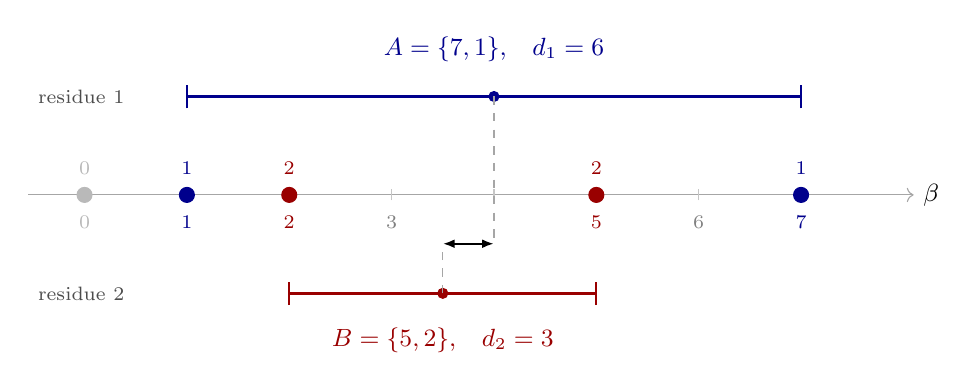
\begin{tikzpicture}[font=\small,x=1.3cm,y=1.0cm]
% --- the two intervals, well clear of the axis ---
\draw[blue!55!black,very thick] (1,1.25) -- (7,1.25);
\draw[blue!55!black,thick] (1,1.10) -- (1,1.40);
\draw[blue!55!black,thick] (7,1.10) -- (7,1.40);
\filldraw[blue!55!black] (4,1.25) circle (1.8pt);
\node[blue!55!black,above=9pt] at (4,1.25) {$A=\{7,1\}$,\quad $d_1=6$};
\draw[red!60!black,very thick] (2,-1.25) -- (5,-1.25);
\draw[red!60!black,thick] (2,-1.40) -- (2,-1.10);
\draw[red!60!black,thick] (5,-1.40) -- (5,-1.10);
\filldraw[red!60!black] (3.5,-1.25) circle (1.8pt);
\node[red!60!black,below=9pt] at (3.5,-1.25) {$B=\{5,2\}$,\quad $d_2=3$};
% --- the beta line ---
\draw[->,gray!70] (-0.55,0) -- (8.1,0) node[right,black]{$\beta$};
\foreach \b in {0,...,7} \draw[gray!45] (\b,-0.07) -- (\b,0.07);
\foreach \b in {3,6} \node[gray,font=\scriptsize,below=4pt] at (\b,0) {$\b$};
\foreach \b/\c/\r in {7/blue!55!black/1, 5/red!60!black/2, 2/red!60!black/2,
                      1/blue!55!black/1, 0/gray!55/0}
  {\filldraw[\c] (\b,0) circle (2.7pt);
   \node[\c,font=\scriptsize,below=4pt] at (\b,0) {$\b$};
   \node[\c,font=\scriptsize,above=4pt] at (\b,0) {$\r$};}
% --- the centres and their distance ---
\draw[gray!70,dashed] (4,1.25) -- (4,-0.62);
\draw[gray!70,dashed] (3.5,-1.25) -- (3.5,-0.62);
\draw[{Latex[length=1.5mm]}-{Latex[length=1.5mm]},thick] (3.5,-0.62) -- (4,-0.62);
\node[font=\scriptsize,gray!60!black,anchor=west] at (-0.55,1.25) {residue $1$};
\node[font=\scriptsize,gray!60!black,anchor=west] at (-0.55,-1.25) {residue $2$};
\end{tikzpicture}
\caption{The mechanism for $t=3$, $\lambda=(3,2)$: here $N=5$, $\beta=(7,5,2,1,0)$ with residues
$(1,2,2,1,0)$ modulo $3$, so no class is empty and two classes have size two. The three arguments of
\eqref{eq:main} are the two interval lengths and twice the distance between the interval centres;
the short double arrow marks that distance, here $\tfrac12$, so that $d_3=1$.}
\label{fig:intervals}
\end{figure}

\begin{example}
For $t=3$, $\lambda=(3,2)$ as in Figure \ref{fig:intervals}, $(d_1,d_2,d_3)=(6,3,1)$ and
\[
\Phi_3\bigl((3,2);z\bigr)=\varepsilon\,
\frac{\sinh(3\theta)\sinh(\theta/2)}{\sinh(3\theta/2)\sinh\theta}.
\]
For $t=3$, $\lambda=(3,1)$ the profile is the size-three one, $(d_1,d_2,d_3)=(3,3,6)$ and
$\Phi_3=\varepsilon\,\chi_2(z)$. For $t=4$, $\lambda=(1,1,1)$ we have $\beta=(6,5,4,2,1,0)$, the
class $3$ is empty and $\Phi_4=0$.
\end{example}

\subsection{The image of the map}
Theorem \ref{thm:main} sends every partition with at most $N$ rows to three integers, so the whole
family collapses onto a sparse subset of $\ZZ^3$. By Proposition \ref{prop:quotient} the first two
coordinates are multiples of $t$; the third is not a multiple of $t$ except in the size-three
profile, where $d_3=d_1+d_2$. Figure \ref{fig:image} shows the image for $t=3$ and $t=4$, coloured
by the number of partitions collapsing onto each point.

\begin{figure}[t]
\centering
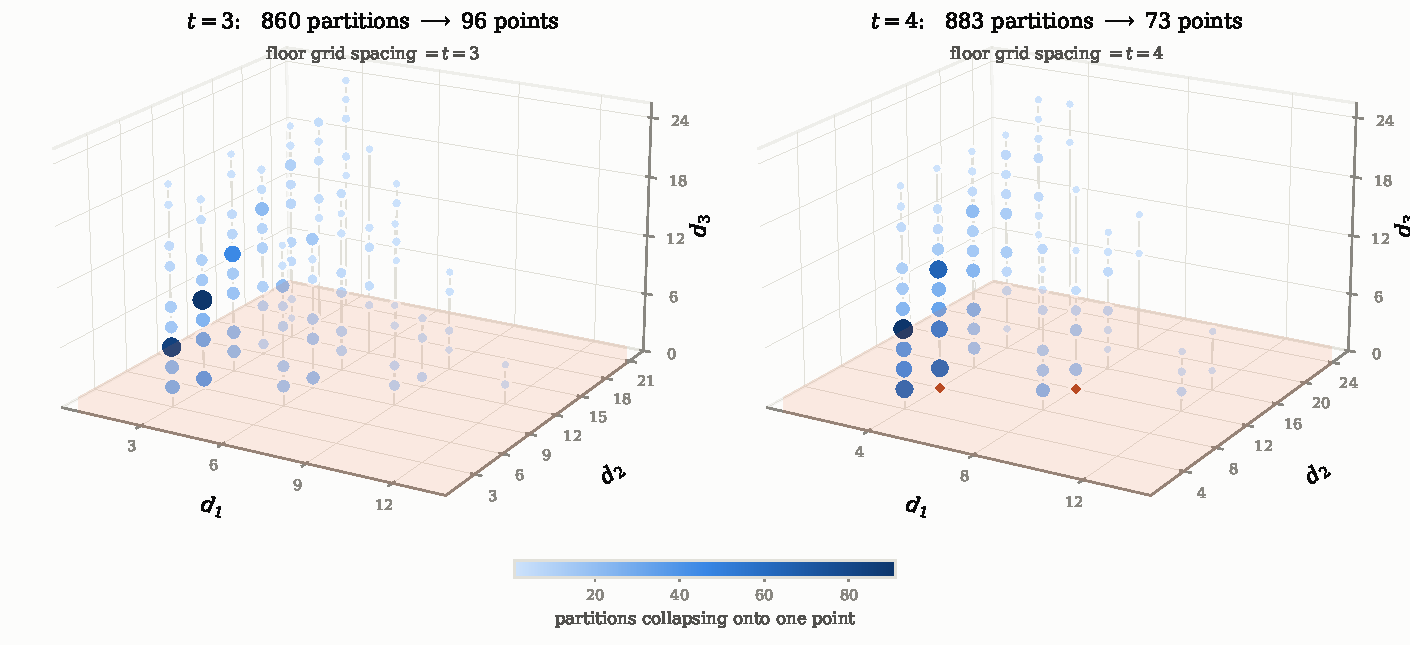
\includegraphics[width=\textwidth]{fig_image.pdf}
\caption{The image of $\lambda\mapsto(d_1,d_2,d_3)$ over all $\lambda$ with $|\lambda|\le20$ and at
most $t+2$ rows, for $t=3$ (left) and $t=4$ (right), taken \emph{up to the exchange of $d_1$ and
$d_2$}, under which \eqref{eq:main} is symmetric; without that identification, and with $A$ and $B$
in the order $r_A\le r_B$ of Theorem \ref{thm:main}, the two panels carry $126$ and $92$ points
rather than $96$ and $73$. The compression is the point of the picture: $860$
partitions land on $96$ triples on the left and $883$ on $73$ on the right, and colour and area give
the number of partitions mapping to each. The floor grid spacing is $t$, since $d_1,d_2\in t\ZZ$ by Proposition
\ref{prop:quotient}; the shaded plane $d_3=0$ is the concentric locus of Corollary \ref{cor:zero},
where $s_\lambda$ vanishes, so those shapes are not in the image and are drawn on the plane as
diamonds instead. The two panels are the two parities, which is the content of Proposition
\ref{rem:lattice}: the odd one carries no diamond, and can carry none; the even one carries two,
between them the images of $32$ partitions.}
\label{fig:image}
\end{figure}

Figure \ref{fig:image} is one half of the picture: it shows which triples occur, not what a triple
hides. Figure \ref{fig:fibres} is the other half. Over each cell of the $(d_1,d_2)$ floor it stands
the column of sizes $|\lambda|$ that land there, so a column is a set of partitions of different
sizes on which $\Phi_t$ takes one and the same value --- and the columns do not thin out as
$|\lambda|$ grows, since the values are confined to a lattice and the partitions are not. The most
visible one is the fibre of the empty partition: at $t=3$ the invariant $I_3=(3,3,2,+1)$ is shared by
$26$ partitions, of $19$ different sizes between $0$ and $20$, so $\Phi_3$ does not distinguish
$\varnothing$ from a shape of twenty boxes.

\begin{figure}[!ht]
\centering
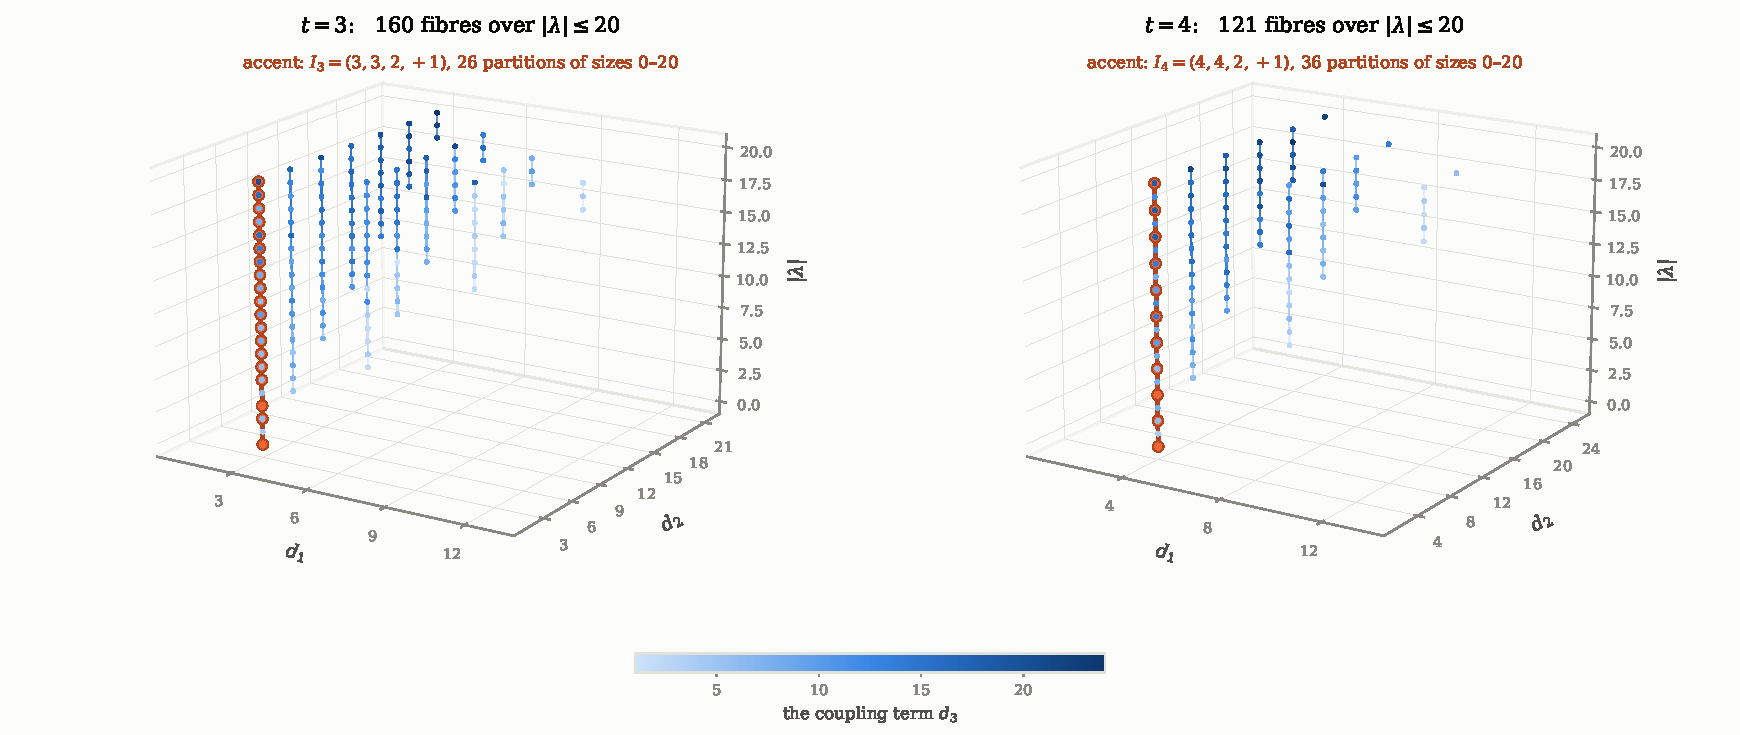
\includegraphics[width=\textwidth]{fig_fibres.pdf}
\caption{The fibres of the evaluation invariant \eqref{eq:invariant}, the complement of Figure
\ref{fig:image}: the same range $|\lambda|\le20$, with the coupling term moved to colour and the
size $|\lambda|$ on the vertical axis. A column is one fibre, so its height is the range of sizes
this alphabet cannot tell apart; the floor ticks are the lattice $t\ZZ$ of Proposition
\ref{prop:quotient}, and only the half $d_1\le d_2$ is occupied because the triple is taken up to the
exchange, as in Figure \ref{fig:image}. That every marker of a column carries the same value is
computed and not assumed: over the $860$ partitions on the left and the $883$ on the right the
bialternant is constant on each fibre to $10^{-37}$. The accent column is the fibre of
$\lambda=\varnothing$.}
\label{fig:fibres}
\end{figure}

Figure \ref{fig:fibres} makes one thing about \eqref{eq:invariant} precise: $I_t$ is complete but
not minimal. The numerator of \eqref{eq:main} is symmetric in $d_1,d_2,d_3$, so the value sees only the multiset
$\{d_1,d_2,d_3\}$ together with the sign, and that is a real reduction --- over $t=4$ and
$|\lambda|\le20$ the $121$ invariants take only $110$ values, while at $t=3$ in the same range the
two counts agree. In the same range no two distinct multisets share a value, so the minimal invariant
of this evaluation is the pair (multiset, sign); we keep the ordered form in \eqref{eq:invariant}
because $d_3$ is the coordinate the reciprocal pair contributes and the other two are not, and
Corollary \ref{cor:fibregf} describes the fibres of either, since the two differ by a symmetry of
the numerator and not by anything the lattice sees.

\begin{proposition}[a shorter form of the sign]\label{rem:sign}
Let the residue profile be non-degenerate and $a_1+a_2\ne b_1+b_2$, and order the two distinguished
classes so that $r_A\le r_B$. Then
\begin{equation}\label{eq:shortsign}
\boxed{\;\;\varepsilon_\lambda\;=\;(-1)^{\lfloor t/2\rfloor}\,\sgn(\sigma)\,(-1)^{\,r_A+r_B}\,
\sgn\bigl(a_1+a_2-b_1-b_2\bigr)\;\;}
\end{equation}
where $\sigma$ is the permutation of \S\ref{sec:background}.
\end{proposition}

\begin{proof}
Let $w$ be the residue word of $\beta(\lambda)$ read in increasing column order. Since $\beta$
decreases with the column index, grouping the parts by class with the values decreasing inside each
class is the stable sort of $w$, so $\sgn(\sigma)=(-1)^{\inv(w)}$. Both sides of
\eqref{eq:shortsign} carry the factor $\sgn(a_1+a_2-b_1-b_2)$, and
$\sgn(a_1-b_1)=(-1)^{[a_1<b_1]}$, so by \eqref{eq:sign} the assertion is equivalent to
\begin{equation}\label{eq:signparity}
j_{A_1}+j_{B_1}+\inv(w)+\inv(b_S)+[a_1<b_1]\;\equiv\;
\Bigl\lfloor\tfrac t2\Bigr\rfloor+t+\binom{N+1}{2}+r_A+r_B \pmod 2 .
\end{equation}

We use one parity count. Let $u$ be a word, $p$ a position, $c=u_p$, and let $I(p)$ be the number of
inversions of $u$ in which $p$ takes part; write $\nu_{<c}$ for the number of letters of $u$ strictly
below $c$ and $e_p$ for the number of occurrences of $c$ strictly before $p$. Putting
$x=\#\{j<p:u_j>c\}$, the positions before $p$ split as $p-1=x+e_p+\#\{j<p:u_j<c\}$ and the letters
below $c$ split as $\nu_{<c}=\#\{j<p:u_j<c\}+\#\{j>p:u_j<c\}$, whence
\begin{equation}\label{eq:parity}
I(p)\;=\;x+\#\{j>p:u_j<c\}\;=\;2x+e_p+\nu_{<c}-(p-1)\;\equiv\;(p-1)+\nu_{<c}+e_p \pmod 2 .
\end{equation}
Since $b_S$ is $w$ with the letters at the positions $j_{A_1}$ and $j_{B_1}$ deleted,
\[
\inv(w)-\inv(b_S)=I(j_{A_1})+I(j_{B_1})
-\bigl[\,\{j_{A_1},j_{B_1}\}\ \text{is an inversion of }w\,\bigr],
\]
and $\inv(w)+\inv(b_S)\equiv\inv(w)-\inv(b_S)$, so \eqref{eq:parity} computes the left-hand side of
\eqref{eq:signparity}.

In the two-class profile $r_A<r_B$, and $w$ carries $r_A$ twice, $r_B$ twice and every other residue
once. Because $\beta$ decreases with the column index, $a_1>a_2$ puts $j_{A_1}$ at the \emph{first}
occurrence of $r_A$, so $e=0$ there, and likewise at $j_{B_1}$. The letters below $r_A$ are one copy
of each of $0,\dots,r_A-1$, so $\nu_{<r_A}=r_A$; those below $r_B$ are the same together with the
second copy of $r_A$, so $\nu_{<r_B}=r_B+1$. The two positions form an inversion exactly when the
larger letter comes first, that is when $j_{B_1}<j_{A_1}$, that is when $a_1<b_1$. Hence
\[
\inv(w)-\inv(b_S)\;\equiv\;(j_{A_1}-1+r_A)+(j_{B_1}-1+r_B+1)+[a_1<b_1]
\;\equiv\;j_{A_1}+j_{B_1}+r_A+r_B+1+[a_1<b_1],
\]
and substituting this in \eqref{eq:signparity} cancels the columns and $[a_1<b_1]$ in pairs, leaving
$\lfloor t/2\rfloor+t+\binom{N+1}{2}\equiv1$.

In the size-three profile $r_A=r_B=:r$ and the class $\{p>q>p'\}$ sits at columns $j_1<j_2<j_3$ with
$A=\{p,q\}$ and $B=\{q,p'\}$, so $j_{A_1}=j_1$ and $j_{B_1}=j_2$ carry the same letter $r$, with
$e=0$ and $e=1$ respectively and $\nu_{<r}=r$ in both; two equal letters are not an inversion, and
$a_1>b_1$. So $\inv(w)-\inv(b_S)\equiv j_1+j_2+1$, which is the displayed expression again because
$r_A+r_B=2r$ and $[a_1<b_1]=0$, and \eqref{eq:signparity} reduces to the same congruence.

Finally $N=t+2$, so that congruence reads $\lfloor t/2\rfloor+t+\binom{t+3}{2}\equiv1$: for $t=2m$
its three terms are $m$, $0$ and $m+1$, and for $t=2m+1$ they are $m$, $1$ and $m$. Both sums are
odd, and the identity holds for every $t\ge2$.
\end{proof}

The ordering by residue is not a convenience, and it is worth saying why. Exchanging the two blocks
negates the sign $\kappa_{11}$ of Lemma \ref{lem:L4} --- through its $\sgn(a_1-b_1)$ factor --- and negates
$\sgn(a_1+a_2-b_1-b_2)$ as well, so it leaves $\varepsilon_\lambda$, which is their product,
invariant; as it must, since $\varepsilon_\lambda$ is attached to $\lambda$. The right-hand side
above is \emph{not} invariant: $(-1)^{r_A+r_B}$ is symmetric, so only its last factor changes sign.
Without a rule fixing which block is $A$, the right-hand side is therefore not a function of
$\lambda$ at all. The hypothesis enters the proof at one point and one only: it is what makes
$\nu_{<r_A}=r_A$ and $\nu_{<r_B}=r_B+1$ rather than the other way round, and dropping it exchanges
those two counts and breaks \eqref{eq:signparity}.

Read the other way round, \eqref{eq:shortsign} says that $\Phi_t$ is a function of a small
combinatorial datum and of nothing else, and it says so for every $t$ rather than over a range: by
Theorem \ref{thm:main} the triple $(d_1,d_2,d_3)$ determines $\Phi_t$ up to sign, and adjoining
$\sgn(\sigma)$, the ordered pair $r_A\le r_B$ and the \emph{orientation}
$\sgn(a_1+a_2-b_1-b_2)$ of $d_3$ determines it outright. The shape of $\lambda$ enters nowhere else.
The orientation is not optional, and that part remains a check rather than a proof: over $t\le6$ and
$|\lambda|\le14$, putting $\sgn(a_1-b_1)$ in its place leaves collisions at $t=2$.

%======================================================================
\section{Proof of Theorem \ref{thm:main}}\label{sec:proof}

The proof uses the Vandermonde determinant, the Laplace expansion, and one cancellation lemma. We
give the steps separately so that a reader checking the ancillary scripts can localise any
disagreement.

What the argument really does is classify rather than compute. Expanding along the $t$ frozen rows
leaves one term for each way of choosing which two columns are \emph{not} frozen, and the excess-two
count says every such choice falls into exactly one of three combinatorial types: none survives
(a residue class is empty), four survive (two classes of size two), or three do (one class of size
three). Everything after that is bookkeeping inside a type, and Lemma \ref{lem:L5} shows the last two
types are one statement seen twice.

\begin{lemma}\label{lem:L1}
Let $S$ be a set of $t$ columns and $M_S=\det(\zeta^{k\beta_j})_{0\le k<t,\,j\in S}$. Then $M_S=0$
unless the residues $\{\beta_j\bmod t:j\in S\}$ are pairwise distinct, in which case
$M_S=(-1)^{\inv(b_S)}V$.
\end{lemma}

\begin{proof}
Since $\zeta^{k\beta_j}=(\zeta^{\beta_j})^k$, the matrix is a Vandermonde matrix in the values
$y_j=\zeta^{\beta_j}$, whose determinant is $\prod_{j<j'}(y_{j'}-y_j)$. The value $y_j$ depends on
$\beta_j$ only modulo $t$, so two columns of $S$ sharing a residue make the determinant vanish. If
the residues are pairwise distinct then $|S|=t$ forces $\{y_j\}_{j\in S}=\zt$ as a set, and the
Vandermonde determinant is alternating in its arguments, so it equals $V$ times the sign of the
permutation sorting $b_S$ increasingly, which is $(-1)^{\inv(b_S)}$.
\end{proof}

\begin{lemma}\label{lem:L2}
$\det\bigl(x_i^{N-j}\bigr)_{i,j=1}^{N}
=(-1)^{\binom t2}\,V\,(z^t-1)(z^{-t}-1)(z-z^{-1})$ for the alphabet
$x=(1,\zeta,\dots,\zeta^{t-1},z,z^{-1})$ in that order.
\end{lemma}

\begin{proof}
The determinant is $\prod_{i<i'}(x_i-x_{i'})$. Pairs inside $\zt$ contribute
$\prod_{k<k'}(\zeta^k-\zeta^{k'})=(-1)^{\binom t2}V$; pairs $(\zeta^k,z)$ contribute
$\prod_k(\zeta^k-z)=(-1)^t(z^t-1)$ and pairs $(\zeta^k,z^{-1})$ contribute $(-1)^t(z^{-t}-1)$; the
last pair contributes $z-z^{-1}$. The two factors $(-1)^t$ cancel.
\end{proof}

\begin{lemma}\label{lem:L3}
Let $\mathcal U$ be the set of pairs $U=\{j_1<j_2\}$ of columns whose complement $S_U$ carries all
$t$ residues. Then
\[
\Phi_t(\lambda;z)=\frac{(-1)^{\,t+\binom{N+1}{2}}}{(z^t-1)(z^{-t}-1)(z-z^{-1})}
\sum_{U\in\mathcal U}(-1)^{\,j_1+j_2+\inv(b_{S_U})}\,f(\beta_{j_1}-\beta_{j_2}).
\]
\end{lemma}

\begin{proof}
Expanding the numerator by Laplace along the first $t$ rows,
\[
\det\bigl(x_i^{\beta_j}\bigr)=\sum_{|S|=t}(-1)^{\binom{t+1}{2}+\sum_{j\in S}j}\,M_S\,C_{S^c},
\]
where for $S^c=\{j_1<j_2\}$ the complementary $2\times2$ minor is
$z^{\beta_{j_1}-\beta_{j_2}}-z^{-(\beta_{j_1}-\beta_{j_2})}=f(\beta_{j_1}-\beta_{j_2})$. By Lemma
\ref{lem:L1} only $S$ with pairwise distinct residues contribute. Writing
$\sum_{j\in S}j=\binom{N+1}{2}-j_1-j_2$ and dividing by Lemma \ref{lem:L2}, the factors $V$ cancel
and $(-1)^{\binom{t+1}{2}-\binom{t}{2}}=(-1)^t$.
\end{proof}

If some $n_i=0$ then no $S$ of size $t$ carries all residues, $\mathcal U=\varnothing$, and
$\Phi_t=0$: this is Theorem \ref{thm:main}(i). Otherwise all $n_i\ge1$ and by \eqref{eq:excess}
either two classes have size two, in which case $S_U$ must drop one element of each and
$|\mathcal U|=4$, or one class has size three, in which case $S_U$ drops two of the three and
$|\mathcal U|=3$.

\begin{lemma}[the column move]\label{lem:L4}
Let $A$ and $B$ be distinct classes of size two, at columns $j_{A_1}<j_{A_2}$ and
$j_{B_1}<j_{B_2}$. For $i,j\in\{1,2\}$ let $U_{ij}$ consist of the column of $a_i$ and the column of
$b_j$, and set $\kappa_{ij}=(-1)^{\,j_{A_i}+j_{B_j}+\inv(b_{S_{U_{ij}}})}\sgn(a_i-b_j)$, so that
the $U_{ij}$ term of Lemma \ref{lem:L3} equals $\kappa_{ij}f(a_i-b_j)$. Then
$\kappa_{ij}=\kappa_{11}(-1)^{i-1}(-1)^{j-1}$.
\end{lemma}

\begin{proof}
Fix $j$ and compare $i=1$ with $i=2$. The sets $S_{U_{1j}}$ and $S_{U_{2j}}$ differ only in that the
first contains the column $j_{A_2}$ and the second the column $j_{A_1}$, and the letter carried is
the residue $r_A$ in both. Passing from one word to the other moves that letter across exactly the
kept columns strictly between $j_{A_1}$ and $j_{A_2}$, and none of those letters equals $r_A$
because the class $A$ has only two elements; each crossing changes the parity of $\inv$. Hence
\[
(-1)^{\inv(b_{S_{U_{1j}}})-\inv(b_{S_{U_{2j}}})}
=(-1)^{(j_{A_2}-j_{A_1}-1)-[\,a_2<b_j<a_1\,]},
\]
using that $\beta$ is strictly decreasing in the column index, so that $j_{B_j}$ lies strictly
between $j_{A_1}$ and $j_{A_2}$ exactly when $a_2<b_j<a_1$. Multiplying by the Laplace factor
$(-1)^{j_{A_1}+j_{A_2}}$,
\[
\frac{\kappa_{1j}}{\kappa_{2j}}
=(-1)^{2j_{A_2}-1}(-1)^{[\,a_2<b_j<a_1\,]}\sgn(a_1-b_j)\sgn(a_2-b_j)=-1,
\]
because $\sgn(a_1-b_j)\sgn(a_2-b_j)=-1$ exactly when $b_j$ lies between $a_2$ and $a_1$. Exchanging
the roles of $A$ and $B$ gives $\kappa_{i1}/\kappa_{i2}=-1$.
\end{proof}

\begin{lemma}\label{lem:L5}
For all $c,p,q$ and all $u,v$,
\begin{align*}
\text{\rm(a)}&\quad \sum_{\epsilon,\eta\in\{\pm1\}}\epsilon\eta\,f(c+\epsilon p+\eta q)=f(c)f(p)f(q),\\
\text{\rm(b)}&\quad f(2u)-f(2u+2v)+f(2v)=-f(u)f(v)f(u+v).
\end{align*}
\end{lemma}

\begin{proof}
For (a), $\sum_{\epsilon,\eta}\epsilon\eta\,z^{c+\epsilon p+\eta q}
=z^{c}\bigl(\sum_\epsilon\epsilon z^{\epsilon p}\bigr)\bigl(\sum_\eta\eta z^{\eta q}\bigr)
=z^{c}f(p)f(q)$, and the same computation for the negative exponents gives
$z^{-c}(-f(p))(-f(q))$; subtract. For (b), put $s=z^u$, $w=z^v$ and expand
$(s-s^{-1})(w-w^{-1})(sw-s^{-1}w^{-1})$: the eight terms recombine as
$(s^2w^2-s^{-2}w^{-2})-(s^2-s^{-2})-(w^2-w^{-2})=f(2u+2v)-f(2u)-f(2v)$.
\end{proof}

\begin{proof}[Proof of Theorem \ref{thm:main}]
In the two-class profile, Lemmas \ref{lem:L3} and \ref{lem:L4} give
\[
\sum_{U\in\mathcal U}(\cdots)=\kappa_{11}\sum_{i,j}(-1)^{i-1}(-1)^{j-1}f(a_i-b_j).
\]
Writing $a_i=\alpha+\epsilon_ip$ and $b_j=\gamma+\eta_jq$ with $p=d_1/2$, $q=d_2/2$ and
$\epsilon=\eta=(+1,-1)$, we have $a_i-b_j=c+\epsilon_ip-\eta_jq$ with $c=\alpha-\gamma$. Replacing
$\eta$ by $-\eta$ turns the sum into $-\sum_{\epsilon,\eta}\epsilon\eta f(c+\epsilon p+\eta q)$,
which is $-f(c)f(p)f(q)$ by Lemma \ref{lem:L5}(a). Since
$(z^t-1)(z^{-t}-1)=2-z^t-z^{-t}=-f(t/2)^2$ and $z-z^{-1}=f(1)$, the two minus signs cancel, and
substituting $f(u)=2\sinh(u\theta)$ the numerical factors cancel and
$\sinh(c\theta)=\sgn(c)\sinh(d_3\theta/2)$, giving \eqref{eq:main} with
$\varepsilon_\lambda=(-1)^{\,t+\binom{N+1}{2}}\kappa_{11}\sgn(a_1+a_2-b_1-b_2)$, which is
\eqref{eq:sign} by the definition of $\kappa_{11}$ in Lemma \ref{lem:L4}.

For the size-three profile $\{p>q>r\}$ at columns $j_1<j_2<j_3$ the same column-move argument
applies, again because no letter strictly between two of these columns carries the class residue,
and gives alternating signs $(\varsigma,-\varsigma,\varsigma)$ for the three terms $f(p-q)$,
$f(p-r)$, $f(q-r)$. By Lemma \ref{lem:L5}(b) with $u=(p-q)/2$, $v=(q-r)/2$ the sum is
$-\varsigma f(u)f(v)f(u+v)$, which is the two-class formula for $A=\{p,q\}$, $B=\{q,r\}$ with
$\varsigma=\kappa_{11}$. Equivalently, the missing fourth selection of the two-class profile would
drop $q$ twice and its term carries $f(0)=0$, so the two profiles are one statement.
\end{proof}

All the statements of this paper were also checked numerically; the counts are collected once, in
\S\ref{sec:verif}, rather than repeated as they arise.

%======================================================================
\section{Independence on the reciprocal locus}\label{sec:independence}

Specializing \eqref{eq:AK53} as in \S\ref{sec:background} gives: for $\ell(\lambda)\le2$,
$s_\lambda(z,\zb,\zt)=s_\lambda(z,\zb)$ if and only if $\lambda=\core_t(\lambda)$. Theorem
\ref{thm:main} evaluates the left-hand side for every $\lambda$, and comparing the two shows that on
the reciprocal locus the criterion acquires further solutions --- exactly one family.

We first isolate when $\Phi_t$ degenerates to a single character. Recall
$\chi_k(z)=(z^{k+1}-z^{-k-1})/(z-z^{-1})$.

\begin{lemma}\label{lem:single}
$\Phi_t(\lambda;z)=\pm\chi_k(z)$ for some $k\ge0$ if and only if the multiset $\{d_1,d_2,d_3\}$
contains $t$ at least twice, and in that case the remaining entry equals $2(k+1)$.
\end{lemma}

\begin{proof}
Put $u=z^{1/2}$, so that $2\sinh(d_i\theta/2)=u^{d_i}-u^{-d_i}$, $2\sinh(t\theta/2)=u^{t}-u^{-t}$ and
$2\sinh\theta=u^{2}-u^{-2}$; all exponents are integers. By \eqref{eq:main}, the asserted equality is
\[
\prod_{i=1}^{3}\bigl(u^{d_i}-u^{-d_i}\bigr)
=\pm\bigl(u^{t}-u^{-t}\bigr)^{2}\bigl(u^{2k+2}-u^{-2k-2}\bigr).
\]
Using $u^{n}-u^{-n}=u^{-n}(u^{2n}-1)$ on each factor and comparing the monomial prefactors gives
$d_1+d_2+d_3=2t+2(k+1)$ together with
\[
\prod_{i=1}^{3}\bigl(u^{2d_i}-1\bigr)=\pm\bigl(u^{2t}-1\bigr)^{2}\bigl(u^{4(k+1)}-1\bigr),
\]
and evaluating at $u=0$ fixes the sign to $+$. Now $u^{2n}-1=\prod_{m\mid 2n}\Phi_m(u)$ with
$\Phi_m$ the cyclotomic polynomials, which are irreducible and pairwise distinct, so by unique
factorization in $\ZZ[u]$ the two sides have the same multiset of cyclotomic factors. On the left
that multiset is $\biguplus_i\{m:m\mid 2d_i\}$ and on the right it is
$2\times\{m:m\mid 2t\}\uplus\{m:m\mid 4(k+1)\}$. Its largest element is $\max_i 2d_i$ on the left and
$\max(2t,4(k+1))$ on the right; deleting the divisor set of that maximum from both sides and
repeating twice more yields
\[
\{2d_1,2d_2,2d_3\}=\{2t,\,2t,\,4(k+1)\}
\]
as multisets, which is the assertion. The converse is the same computation read backwards.
\end{proof}

\begin{theorem}\label{thm:extra}
Let $\ell(\lambda)\le2$. Then $\Phi_t(\lambda;z)=\pm s_\lambda(z,\zb)$ if and only if either
$\lambda=\core_t(\lambda)$, or
\begin{equation}\label{eq:extra}
t\ \text{is even}\quad\text{and}\quad \lambda=\Bigl(\lambda_2+\tfrac{3t}{2}-1,\ \lambda_2\Bigr)
\quad\text{with}\quad \tfrac t2\le\lambda_2\le t-1 .
\end{equation}
In the second case $\{d_1,d_2,d_3\}=\{3t,t,t\}$, while $\core_t(\lambda)=\bigl(\tfrac t2-1+j,j\bigr)$
and $\quot_t(\lambda)$ has the single nonempty component $(2)$, in slot $j=\lambda_2-\tfrac t2$.
\end{theorem}

Figure \ref{fig:locus} is the statement computed rather than asserted: both families are plotted
over a range of $t$, and the odd $t$ where \eqref{eq:extra} cannot occur is drawn as the control.

\begin{figure}[!ht]
\centering

\includegraphics[width=\textwidth]{fig_locus.pdf}
\caption{Theorem \ref{thm:extra}, computed rather than asserted. For every two-row $\lambda$ in
range, both sides of $\Phi_t(\lambda;z)=\pm s_\lambda(z,\zb)$ were evaluated; the partitions where
they agree are plotted and coloured by family. Circles are the $t$-cores, the solutions already
described by \eqref{eq:AK53}; triangles are the extra family \eqref{eq:extra}, which the reciprocal
specialization creates. The odd case $t=3$ is the control: by Theorem \ref{thm:extra} no extra
solution can exist there, and none is found.}
\label{fig:locus}
\end{figure}

\begin{proof}
Since $\ell(\lambda)\le 2$ and $N=t+2$, the beta set is
$\beta(\lambda)=\bigl(A'+t,\;B'+t,\;t-1,t-2,\dots,1,0\bigr)$ where
\[
A':=\lambda_1+1,\qquad B':=\lambda_2,\qquad A'>B'\ge0 .
\]
The block $\{0,1,\dots,t-1\}$ meets every residue class exactly once, so no class is empty and the
two large parts decide the profile. Write $A'=t\alpha+\rho_A$ and $B'=t\gamma+\rho_B$ with
$0\le\rho_A,\rho_B\le t-1$. As $s_\lambda(z,\zb)=\chi_{\lambda_1-\lambda_2}(z)$, Lemma
\ref{lem:single} says that the assertion holds precisely when $\{d_1,d_2,d_3\}$ contains $t$ twice
and the third entry is $2(\lambda_1-\lambda_2+1)=2(A'-B')$.

\emph{Case $\rho_A=\rho_B=:\rho$.} One class has size three, namely $\{A'+t,B'+t,\rho\}$, and by
Theorem \ref{thm:main} the three arguments are
$d_1=A'-B'$, $d_2=B'+t-\rho=t(\gamma+1)$, $d_3=A'+t-\rho=t(\alpha+1)$. Here $t\mid A'-B'$, say
$A'-B'=ts$ with $s\ge1$. The pair $d_2=d_3=t$ forces $\alpha=\gamma=0$, hence $A'=B'$, excluded.
The pair $d_1=d_3=t$ forces $s=1$ and $\alpha=0$, hence $A'<t$ and $A'=B'+t\ge t$, excluded. The pair
$d_1=d_2=t$ forces $s=1$ and $\gamma=0$, i.e. $A'=B'+t$ with $B'<t$; then $\alpha=1$ and the third
entry is $d_3=2t=2(A'-B')$, as required. So this case contributes exactly the $\lambda$ with
$A'=B'+t$, $B'<t$.

\emph{Case $\rho_A\ne\rho_B$.} Two classes have size two, namely $\{A'+t,\rho_A\}$ and
$\{B'+t,\rho_B\}$, and the three arguments are
\[
d_A=t(\alpha+1),\qquad d_B=t(\gamma+1),\qquad
d_3=\bigl|\,t(\alpha-\gamma)+2(\rho_A-\rho_B)\,\bigr| .
\]
If $d_A=d_B=t$ then $\alpha=\gamma=0$, so $A',B'<t$ and $d_3=2|\rho_A-\rho_B|=2(A'-B')$
automatically: every such $\lambda$ is a solution. Otherwise exactly one of $d_A,d_B$ equals $t$ and
$d_3=t$. If $\alpha=0$ and $\gamma\ge1$ then $|-t\gamma+2(\rho_A-\rho_B)|=t$ with
$|\rho_A-\rho_B|\le t-1$ forces $\gamma=2$ and $\rho_A-\rho_B=t/2$; but then
$\lambda_1=A'-1=\rho_A-1<t$ while $\lambda_2=B'\ge2t$, contradicting $\lambda_1\ge\lambda_2$. If
$\gamma=0$ and $\alpha\ge1$ then $|t\alpha+2(\rho_A-\rho_B)|=t$ forces, for $\alpha=1$,
$\rho_A=\rho_B$ (excluded), and for $\alpha=2$,
\[
\rho_B-\rho_A=\tfrac t2,
\]
which requires $t$ even; $\alpha\ge3$ gives $|2(\rho_A-\rho_B)|\ge2t$, impossible. So $A'=2t+\rho_A$,
$B'=\rho_B=\rho_A+\tfrac t2$, whence
\[
\lambda_1=2t+\rho_A-1,\qquad \lambda_2=\rho_A+\tfrac t2,\qquad
\lambda_1-\lambda_2=\tfrac{3t}{2}-1,
\]
and $\rho_B\le t-1$ gives $0\le\rho_A\le\tfrac t2-1$, i.e. $\tfrac t2\le\lambda_2\le t-1$. The
remaining entry is $d_A=t(\alpha+1)=3t=2(\lambda_1-\lambda_2+1)$, as required. This is
\eqref{eq:extra}.

It remains to identify the solutions collected in the first case of each analysis with the
$t$-cores. For $\ell(\lambda)\le2$ the beta set in two slots is $(A',B')$, and $\lambda$ is a
$t$-core if and only if neither beta number can be lowered by $t$ into an unoccupied nonnegative
position, i.e. if and only if $B'<t$ and either $A'<t$ or $A'=B'+t$. These are exactly the two
families found above. Finally, in case \eqref{eq:extra} the class $\rho_A$ carries
$\{2t+\rho_A+t,\rho_A\}$, so its quotient component is $(2)$, every other component is empty, and
the core is as stated.
\end{proof}


\begin{remark}\label{rem:why}
Theorem \ref{thm:extra} is stated up to sign because that is what Lemma \ref{lem:single} controls;
over two-row shapes with $t\le8$ the sign is $+1$ at every solution, so there the equality holds on
the nose.

The extra family belongs to the specialization rather than to the alphabet. The step is
\cite[Lemma 5.2]{AK25}, on which \cite[Theorem 5.3]{AK25} rests: it reduces the independence to the
vanishing of $s_{\lambda/\mu}$ at the twisted alphabet for all $\mu\subsetneq\lambda$, and the
reduction uses the linear independence of the universal characters $f_\mu$ in the free variables. On the reciprocal locus $s_\mu(z,\zb)=\chi_{\mu_1-\mu_2}(z)$
depends only on $\mu_1-\mu_2$, so $s_{(1)}$, $s_{(2,1)}$ and $s_{(3,2)}$ agree there and that
independence is not available; Theorem \ref{thm:extra} measures the difference. A control confirms
the reading: for $\lambda=(3,1)$ and $t=2$ one has $s_\lambda(\zt,z,\zb)=s_\lambda(z,\zb)$, while
$s_\lambda(\zt,x,y)\ne s_\lambda(x,y)$ for free $x,y$.
\end{remark}

So the criterion does not survive the specialization unchanged, and what it acquires is small and
nameable: one family, for two-row shapes, indexed by an order-two element of the residue lattice and
classified by its core and quotient. The extra solutions belong to the reciprocal locus, not to the
alphabet --- they exist because a specialization has removed a linear independence the original
argument used, and that missing step is exactly what Theorem \ref{thm:extra} measures.

%======================================================================
\section{An enumeration in which a parameter survives}\label{sec:enum}

Expanding $s_\lambda$ over semistandard tableaux turns Theorem \ref{thm:main} into a product formula
for a weighted count. Let $m_k(T)$ be the number of entries equal to $k$ in $T$.

\begin{corollary}\label{cor:enum}
Expanding $s_\lambda$ over semistandard tableaux and applying Theorem \ref{thm:main}: for every
$t\ge2$ and every $\lambda\in\PP_{t+2}$,
\[
\sum_{T\in\mathrm{SSYT}(\lambda,\,t+2)}
\zeta^{\,\sum_{k=1}^{t}(k-1)m_k(T)}\;z^{\,m_{t+1}(T)-m_{t+2}(T)}
\;=\;\varepsilon_\lambda\,
\frac{\sinh(d_1\theta/2)\sinh(d_2\theta/2)\sinh(d_3\theta/2)}{\sinh^2(t\theta/2)\sinh\theta}.
\]
\end{corollary}

For $t=2$ the weight is $(-1)^{m_2(T)}$, and if $\lambda=(c^r)$ is rectangular then
$\mathrm{SSYT}(\lambda,4)$ is in bijection with plane partitions in an $r\times(4-r)\times c$ box,
equivalently with lozenge tilings of a hexagon. Corollary \ref{cor:enum} is then a
$(-1)$-enumeration of those objects \emph{refined by a free parameter} $z$, which records the
difference between the numbers of entries $3$ and $4$. Setting $z=1$ recovers the plain signed
count, which by \eqref{eq:main} equals $\pm d_1d_2d_3/(2t^2)$: for $r=2$, $c=2$ it is $4$; for
$r=2$, $c=4$ it is $9$; for $r=3$, $c=3$ it is $-6$.

\begin{example}\label{ex:boxes}
Taking $\lambda=(c^{\,r})$ with $1\le r\le4$ and $t=2$, the shape has at most four rows, the tableaux
are the plane partitions in an $r\times(4-r)\times c$ box, and the closed form gives the signed
counts of Figure \ref{fig:signed}. Reading it off:
\[
\begin{array}{ll}
1\times3\times c: & \bigl\lfloor (c+2)^2/4\bigr\rfloor,\\[2pt]
2\times2\times c: & (c/2+1)^2 \text{ for } c \text{ even},\qquad 0 \text{ for } c \text{ odd},\\[2pt]
3\times1\times c: & (-1)^c\bigl\lfloor (c+2)^2/4\bigr\rfloor,\\[2pt]
4\times0\times c: & (-1)^c .
\end{array}
\]
The third row is the transpose of the first, which is why the magnitudes agree; the fourth is the
degenerate box, where $s_{(c^4)}(x)=(x_1x_2x_3x_4)^c$ and the alphabet has determinant $-1$. We do
not claim these particular counts as new --- the boxes are small and the sign here is the
specialization $x_2=-1$, not the complementation sign of Kuperberg's $(-1)$-enumerations --- and we
record them only to show what the theorem produces. What does appear to be new is that each of them
is the $z\mapsto1$ value of a one-parameter refinement with the same product formula.
\end{example}

The perfect squares in Example \ref{ex:boxes} are not an accident of small cases: they are what the
interval reading of \S\ref{sec:intervals} says a rectangle must produce.

\begin{proposition}\label{prop:rect}
Let $t=2$ and $\lambda=(c^{\,r})$ with $1\le r\le4$. Then one of $d_1,d_2,d_3$ equals $2$, and:
\begin{enumerate}
\item[\rm(i)] if $r=4$, all three equal $2$ for \emph{every} $c$ and the count is $(-1)^c$; this is
the full rectangle, where $s_{(c^4)}(x)=(x_1x_2x_3x_4)^{c}$ collapses to a monomial and the alphabet
contributes only its determinant;
\item[\rm(ii)] if $r\le3$ and $c$ is even, the other two are both equal to $c+2$, so the two
intervals have the \emph{same length} and the signed count is the perfect square
$\bigl(\tfrac{c+2}{2}\bigr)^2$;
\item[\rm(iii)] if $c$ is odd and $r=2$, the two intervals are \emph{concentric} and the count is $0$;
\item[\rm(iv)] if $c$ is odd and $r\in\{1,3\}$, the other two are $c+1$ and $c+3$, and the count is
$\pm\tfrac{(c+1)(c+3)}{4}=\pm\bigl\lfloor\tfrac{(c+2)^2}{4}\bigr\rfloor$.
\end{enumerate}
Case {\rm(i)} is not a degeneration of the interval triple but a collapse of the shape itself, and it
is the only case in which the parity of $c$ plays no role.
\end{proposition}

\begin{proof}
For $\lambda=(c^{\,r})$ the beta set consists of two blocks of consecutive integers, namely
$c+3,c+2,\dots,c+4-r$ and $3-r,2-r,\dots,0$; residues alternate along each block, which is what
forces the coincidences. Explicitly, for $r=1,2,3,4$ the beta set is $(c+3,2,1,0)$, $(c+3,c+2,1,0)$,
$(c+3,c+2,c+1,0)$ and $(c+3,c+2,c+1,c)$. Splitting each by parity gives, for $c$ even,
\[
\{c{+}3,1\},\{2,0\};\qquad \{c{+}3,1\},\{c{+}2,0\};\qquad \{c{+}3,c{+}1\},\{c{+}2,0\};\qquad
\{c{+}3,c{+}1\},\{c{+}2,c\},
\]
whence $(d_1,d_2,d_3)$ equals $(c{+}2,2,c{+}2)$, $(c{+}2,c{+}2,2)$, $(2,c{+}2,c{+}2)$ and
$(2,2,2)$ respectively; in each case the product over $2t^2=8$ is $\bigl(\tfrac{c+2}{2}\bigr)^2$,
resp. $1$. For $c$ odd and $r=2$ the split is $\{c{+}3,0\},\{c{+}2,1\}$, so
$d_3=|c{+}3+0-c{-}2-1|=0$: the intervals are concentric and Corollary \ref{cor:zero} applies. For
$c$ odd and $r=1,3$ the parity puts three beta numbers in one class, $\{c{+}3,2,0\}$ and
$\{c{+}3,c{+}1,0\}$ respectively, and the size-three profile gives $(c{+}1,2,c{+}3)$ and
$(2,c{+}1,c{+}3)$, with product over $8$ equal to $\tfrac{(c+1)(c+3)}{4}$. For $c$ odd and $r=4$ the
four beta numbers are again consecutive, so the split is $\{c{+}3,c{+}1\},\{c{+}2,c\}$ and the triple
is $(2,2,2)$ exactly as for $c$ even: at full height the answer does not see the parity of $c$, which
is why $r=4$ is separated out.
\end{proof}

So the square is the square of half the common interval length, the zeros are the concentric
configurations, the quarter-squares are the case where the two lengths differ by $2$, and at full
height all three intervals coincide, the shape becomes a monomial and only a sign survives. Which
pair of the three coincides rotates with $r$, which is why the same value appears in different
columns of Figure \ref{fig:signed}.

\begin{figure}[t]
\centering

\includegraphics[width=\textwidth]{fig_signed.pdf}
\caption{The signed counts of Example \ref{ex:boxes}: the value of Corollary \ref{cor:enum} at
$z=1$ and $t=2$ for the rectangular shapes $\lambda=(c^{\,r})$, that is the $(-1)$-enumeration of
plane partitions in an $r\times(4-r)\times c$ box. Every entry is the closed form
$\varepsilon_\lambda\,d_1d_2d_3/(2t^2)$, cross-checked against a direct enumeration of the tableaux.
The row $r=2$ vanishes for odd $c$ and is a perfect square for even $c$.}
\label{fig:signed}
\end{figure}

The $(-1)$-enumeration literature --- Kuperberg \cite{Kup02}, Eisenk\"olbl \cite{Eis07} building on
Stanley \cite{Sta86} and on the Pfaffian identities of \cite{IOTZ06}, Ciucu, Krattenthaler ---
computes such signed counts with the variables specialized to $1$. Keeping the parameter free appears not to have
been recorded, and it is the feature that distinguishes the present alphabet: the reciprocal pair is
precisely the mechanism that lets one variable survive the signed enumeration.

A refinement of a different kind is standard in the ribbon world, and it is worth saying which:
the LLT polynomials of Lascoux, Leclerc and Thibon \cite{LLT97} grade ribbon tableaux by a spin
statistic. That $q$ is an extra grading rather than a letter, and the object it grades is indexed by
a tuple of shapes; the parameter here is the alphabet's own and what carries it is a single
$s_\lambda$. The two refine different things, which is why we put the point narrowly: it is the
reciprocal pair, and not a statistic, that keeps a variable alive through the signed count.

A signed enumeration with a product formula asks for a sign-reversing involution, and the obstruction
is specific: the involution must preserve $m_{t+1}-m_{t+2}$, or the free parameter is not carried
across, and neither Bender--Knuth moves nor the single-cell toggle do. The construction in
\cite{KumariThesis} of a fixed-point-free sign-reversing involution on semistandard tableaux over a
$\pm$-paired alphabet, whose fixed set is the domino-tileable tableaux, does have the required
property in its $i=1$ instance: it touches only cells holding $1$ or $2$, hence preserves
$z^{m_3-m_4}$ and reverses $(-1)^{m_2}$. The triple product it would have to land on is the one of
Corollary \ref{cor:chars}, which at $t=2$ is a product of three $\mathfrak{sl}_2$ characters on the
nose, so the missing bijection is a Clebsch--Gordan statement. That is one half. The other is the
cancellation across the
splitting of the alphabet, and at $t=2$ it concerns a single one-parameter family. By
\eqref{eq:threestep} below,
\[
s_\lambda(1,-1,z,\zb)=\sum_{\ell(\nu)\le2}s_{\lambda/\nu}(1,-1)\,\chi_{\nu_1-\nu_2}(z),
\]
and an involution carrying the parameter must preserve $k=\nu_1-\nu_2$, since that is the index of
the character its term sits on. For fixed $k$ the admissible $\nu$ are exactly $(m+k,m)$ with
$m\ge0$, so that cancellation is a statement about one word.

The size of the terms is classical. Littlewood's theorem has a skew form --- $\varphi_t
s_{\lambda/\nu}$ vanishes unless $\lambda/\nu$ is tileable by $t$-ribbons, and is otherwise a ribbon
sign times a product over the quotient --- due to Macdonald \cite[p.~91]{Mac95}, and proved there by
the same Jacobi--Trudi route we take below; the case where $\nu$ is the $t$-core is Farahat's. At
$t=2$ on our alphabet it gives $\sigma_m\in\{0,\pm1\}$ at once. What is not classical is how the
sign moves with $m$, and that is what the involution needs.

\begin{figure}[t]
\centering

\includegraphics[width=\textwidth]{fig_runs.pdf}
\caption{Proposition \ref{rem:involution}, drawn. For each $k$ the admissible $\nu$ are the single
family $(m+k,m)$, and $\sigma_m=s_{\lambda/(m+k,m)}(1,-1)$ is plotted against $m$ and $k$; the grey
dots are the zeros. Every bar has height exactly $\pm1$, which is part (i): the terms are a set, so
the cancellation the enumeration asks for is a matching and not something carrying multiplicity. On
the left every $k$ is even and the colour alternates along each run, which is part (iii) and what
makes $m\leftrightarrow m+1$ sign-reversing; where a run ends, a zero ends it. On the right every
$k$ is odd and no two nonzero terms are adjacent, which is part (ii): the runs have length one and
there is nothing to cancel.}
\label{fig:runs}
\end{figure}

\begin{proposition}[the runs alternate]\label{rem:involution}
Let $t=2$, let $k\ge0$, and put $\sigma_m=s_{\lambda/(m+k,m)}(1,-1)$ for $m\ge0$. Then
\begin{enumerate}
\item[\rm(i)] $\sigma_m\in\{0,\pm1\}$ --- this part is Macdonald's, not ours;
\item[\rm(ii)] if $k$ is odd, no two consecutive $\sigma_m$ are nonzero;
\item[\rm(iii)] if $\sigma_m$ and $\sigma_{m+1}$ are both nonzero then $\sigma_{m+1}=-\sigma_m$.
\end{enumerate}
Consequently, pairing $m$ with $m+1$ inside each maximal run of consecutive nonzero $\sigma$ is a
sign-reversing involution, and $\sum_m\sigma_m$ is the signed count of the runs of odd length.
\end{proposition}

The three parts are visible at once in Figure \ref{fig:runs}: the bar heights are part {\rm(i)}, the
gaps on the odd panel are part {\rm(ii)}, and the alternation of colour along each run is part
{\rm(iii)}.

\begin{proof}
Write $\beta_i=\lambda_i-i$ and $c_j=\nu_j-j$, and take the Jacobi--Trudi matrix of
$s_{\lambda/\nu}$ in $n\ge\ell(\lambda)$ rows. Since $h_j(1,-1)=1$ for $j\ge0$ even and $0$
otherwise,
\begin{equation}\label{eq:betaJT}
M_{ij}=\bigl[\beta_i\ge c_j\bigr]\cdot\bigl[\beta_i\equiv c_j \bmod 2\bigr],\qquad
\sigma_m=\det M .
\end{equation}
The second factor says that column $j$ is supported on the rows of one parity class, the class of
$c_j$; and since $\beta_1>\dots>\beta_n$, inside that class the first factor cuts an \emph{initial
segment}. Order the rows by parity class: $M$ becomes block diagonal, so it is singular unless each
class carries as many columns as it has rows, and inside a class it is the staircase
$\bigl[\,\text{the rank of }i\text{ in its class}\le\ell_j\bigr]$ of the segment lengths $\ell_j$. That staircase is singular if two
lengths agree or one is $0$, and otherwise the lengths are a permutation of $1,\dots,e$ and its
determinant is the sign of that permutation. This gives (i), which is \cite[p.~91]{Mac95} in this
case; we re-derive it because the $\beta$-form \eqref{eq:betaJT} is what (ii) and (iii) rest on.

For $\nu=(m+k,m)$ we have $c_1=m+k-1$, $c_2=m-2$ and $c_j=-j$ for $j\ge3$. So $c_1-c_2=k+1$, and
passing from $m$ to $m+1$ raises $c_1$ and $c_2$ by one and leaves every other column alone: exactly
the first two columns change parity class.

If $k$ is odd then $c_1\equiv c_2$, so columns $1$ and $2$ lie in the same class and both leave it.
That class's column count changes by two while its row count does not, so at most one of $\sigma_m$,
$\sigma_{m+1}$ can be nonzero, which is (ii).

If $k$ is even then $c_1\not\equiv c_2$ and the two columns exchange classes. Suppose both are
nonzero. In the class of $c_1$ the columns are column $1$ together with a set of columns $j\ge3$
that does not move; by (i) the lengths are a permutation of $1,\dots,e$ before and after, and the
fixed columns contribute the same lengths to both, so the length column $2$ brings in equals the one
column $1$ took away --- and symmetrically in the other class. Each class therefore sees the same
lengths in the same order of columns, and both block determinants are unchanged. What does change is
the shuffle separating the two classes of columns: columns $1$ and $2$ are adjacent and exchange
membership, which alters the number of inversions of that shuffle by exactly one. Hence
$\sigma_{m+1}=-\sigma_m$, which is (iii).
\end{proof}

\begin{remark}[the sign here is the sign of Theorem \ref{thm:main}]\label{rem:onesign}
Write $\sigma_\nu$ for the permutation of \S\ref{sec:background} attached to a partition $\nu$: the
one sorting $\beta$ by residue class, which Proposition \ref{rem:sign} places inside
$\varepsilon_\lambda$. The terms of Proposition \ref{rem:involution} are values of that same sign.
Indeed $\sigma_m$ vanishes unless $\core_2(\lambda)=\core_2(\nu)$ and both components of the skew
$2$-quotient are horizontal strips, and equals $\sgn(\sigma_\lambda)\sgn(\sigma_\nu)$ when it does
not --- the identity $\sgn(\sigma_\lambda)\sgn(\sigma_\nu)=(-1)^{\sum_B\mathrm{ht}(B)}$ being the
ribbon sign of \cite[p.~91]{Mac95} written as a sorting sign, which is
\cite[Lemma 6.3]{KumariThesis}. Parts {\rm(ii)} and {\rm(iii)} are
then one statement about $\sigma_\nu$ alone: as $\nu=(m+k,m)$ moves to $(m+k+1,m+1)$,
$\sgn(\sigma_\nu)$ reverses for $k$ even and is constant for $k$ odd. So the permutation that
carries the sign of the main theorem is the permutation that makes the involution of this section
alternate; the two halves of the paper are signed by one object.
\end{remark}

The pairing is a bijection of tableaux and not only of terms, which is what carries the parameter. A
semistandard tableau of shape $(a,b)$ in the letters $3,4$ has second row $4^{\,b}$ and first row
$3^{\,p}4^{\,a-p}$ with $b\le p\le a$, of weight $z^{2p-a-b}$; adjoining a first column
$\left(\begin{smallmatrix}3\\4\end{smallmatrix}\right)$ sends it to the tableau of shape
$(a+1,b+1)$ with $p+1$ in place of $p$, and $2(p+1)-(a+1)-(b+1)=2p-a-b$, so $m_3-m_4$ is preserved
exactly. Composing that with Proposition \ref{rem:involution} pairs the terms of Corollary
\ref{cor:enum} in the way the enumeration asks for.

One half is not ours, and we say which. Proposition \ref{rem:involution} disposes of the cancellation
across $\nu$; the cancellation \emph{inside} each $s_{\lambda/\nu}(1,-1)$ is
\cite{KumariThesis}, and the two fit together. There, at $n=1$, the alphabet is $(x,-x)$ and the
weight of a two-letter filling is $(-1)^{c_2}$, which is $\sigma_m$; the involution
\cite[Lemma 2.18]{KumariThesis} is fixed-point-free on the fillings that are \emph{not coverable},
so the sum reduces to the coverable ones, which \cite[Lemma 2.16]{KumariThesis} matches with domino
tableaux. What makes the reduction usable here is \cite[Lemma 2.14]{KumariThesis}: the parity of the
number of vertical dominoes does not depend on the tableau, so every survivor carries the same sign
and $\sigma_m=\pm\#\{\text{coverable fillings}\}$. With part (i) that forces the count to be at most
one, so the fixed set is a single filling when $\sigma_m\ne0$ and empty otherwise --- checked
directly over the $1134$ skew shapes with at most four rows and $|\lambda|\le10$, where the two
counts agree without exception.

At $t=2$ the involution the enumeration asks for therefore exists: cancel inside each $\nu$ by
\cite[Lemma 2.18]{KumariThesis}, pair what is left across $\nu$ by Proposition \ref{rem:involution},
and carry the parameter by the column $\left(\begin{smallmatrix}3\\4\end{smallmatrix}\right)$. Its
fixed points are one filling for each run of odd length, and Corollary \ref{cor:enum} counts them.
The construction is Kumari's; the assembly is ours.

%======================================================================
\section{The factorization is isolated}\label{sec:sharp}

A factorization is only a result if it is not a specialization of a known one, and it is only a
\emph{sharp} result if the alphabet cannot be deformed. There are four deformations of
\eqref{eq:object}, and all four destroy the product.

The evidence in this section is computational, and we label it as such: none of (D1)--(D4) below is
a theorem, and in particular we prove no no-go statement. What we assert is that the identity
\eqref{eq:main} is false for each deformed alphabet, which a single counterexample settles, and we
give counts to indicate how far from true it is.

\begin{itemize}
\item[\rm(D1)] \emph{More reciprocal pairs.} For $s_\lambda(\zt,z_1,z_1^{-1},\dots,z_r,z_r^{-1})$
with $r\ge2$ there is no product law: typical values carry one large irreducible factor, and the only
factors that split off are binomials in the rotated variables $z_1z_2$ and $z_1z_2^{-1}$, that is,
the couplings between the pairs' $u(1)$ charges. What does survive every $r$ is the \emph{zero
locus}, and Theorem \ref{thm:zeros} determines it; the product is the rank-one accident and the
vanishing is the part that generalizes.
\item[\rm(D2)] \emph{More orbit variables.} For $s_\lambda(X,\zeta X,\dots,\zeta^{t-1}X,z,z^{-1})$
with $|X|=n\ge2$ there is no product law. At $t=2$, $n=2$ the value for $\lambda=(2)$ is
$(x^2z^2+y^2z^2+z^4+z^2+1)/z^2$, irreducible over $\mathbb Q$; for $\lambda=(2,2)$ it is
$(x^2+y^2+z^2)(x^2z^2+y^2z^2+1)/z^2$, two factors rather than three; and for $\lambda=(3,1)$ it is
again irreducible. By contrast, with the pair deleted the same alphabet obeys \cite[Theorem
2.3]{AK25}: $s_{(2)}(x,y,-x,-y)=x^2+y^2$ and $s_{(2,2)}(x,y,-x,-y)=(x^2+y^2)^2$.
\item[\rm(D3)] \emph{The orbit replaced by a coset.} For $\zeta'\zt$ with $\zeta'=e^{\pi i/t}$, the
odd powers of a primitive $2t$-th root of unity --- the twist of \cite[\S3]{AK25}, and for $t$ even
the full set of primitive $2t$-th roots studied in \cite{HI24} --- the identity fails, vanishing
criterion included.
\item[\rm(D4)] \emph{The reciprocal pair replaced by a free pair.} $s_\lambda(\zt,x,y)$ is
generically irreducible.
\end{itemize}

Counts for (D3) and (D4), over $t=2,\dots,6$ and $|\lambda|\le10$: the identity holds in all $600$
cases for \eqref{eq:object}, in $383$ of $600$ for (D3), and in $200$ of $600$ for (D4). The test is
therefore capable of failing, which is the point of quoting the first row.

One reading of the proof accounts for all four. Splitting the alphabet and applying Theorem
\ref{thm:LR} to the frozen half gives, for any free alphabet $B$,
\begin{equation}\label{eq:threestep}
s_\lambda(\zt\cup B)=\sum_{\nu}s_{\lambda/\nu}(\zt)\,s_\nu(B)=\sum_\nu\varepsilon_\nu\,s_\nu(B),
\qquad \varepsilon_\nu\in\{0,\pm1\},
\end{equation}
the coefficients being ribbon signs: that the skew evaluation $s_{\lambda/\nu}(\zt)$ is $0$ or a
ribbon sign is the skew form of Theorem \ref{thm:LR}, due to Macdonald \cite[p.~91]{Mac95}. Now
$B=(z,z^{-1})$ has exactly two letters and they are
reciprocal, so $s_\nu(B)=\chi_{\nu_1-\nu_2}(z)$ is a \emph{single} $\mathfrak{sl}_2$ character
depending on one difference, and the short signed sum collapses. Step one requires the frozen half
to be a full orbit, since Theorem \ref{thm:LR} needs the rows to meet every residue class exactly;
a coset does not, which is (D3). Step two requires the free half to be exactly one reciprocal pair:
a free pair has $\det=xy$ and couples to both central charges, which is (D4), and enlarging the free
half --- by more pairs, or by more orbit variables, which enlarges $\nu$ --- makes $s_\nu(B)$ cease
to be a single character and the sum cease to collapse, which is (D1) and (D2). \emph{The four
failures are one condition seen from four sides.}

\begin{remark}
Equivalently: the reciprocal pair contributes exactly \emph{one} coupling, the cross term $d_3$,
because $\det=1$ prevents it from seeing the two central charges separately. This is why there are
three factors and not two, and Ayyer--Kumari's factorizations, which are products over quotient
components with no coupling at all, are the case where that contribution is absent.
\end{remark}

\begin{remark}[a representation-theoretic reading]\label{rem:twining}
The alphabet \eqref{eq:object} is closed under inversion, hence a torus element of $O(N)$, and its
determinant is $(-1)^{t+1}$. For even $t$ it therefore lies in the non-identity component, where a
character is a \emph{twining} character; the identity computing such characters by folding is due to
Jantzen \cite{Jantzen} and, in the form closest to this one, to Kumar--Lusztig--Prasad \cite{KLP},
the relevant folded algebra being the orbit Lie algebra. Our restriction is reducible, so it is
reached from theirs by one step of Clifford theory. We record this because Ciucu--Krattenthaler
\cite{CK09} wrote that they could not offer a representation-theoretic interpretation of their
factorizations, and \cite{AB19} and \cite{AK25} repeat that it is still missing; the reading here is
of that kind. The mechanism is entirely theirs, and the proof above does not use it. Lemma
\ref{lem:AtoSp} makes the reading concrete for the alphabet \eqref{eq:psir}, where the folded algebra
is $C_r$ and the twining character is a symplectic character on the nose.
\end{remark}

%======================================================================
\section{The zero locus survives every $r$}\label{sec:zeros}

This section is past the factorization, and reads differently from the seven before it. Those prove
statements about an identity; this one asks what is left when the identity is gone, and the answer is
a locus rather than a formula --- proved in one direction for every $r$, in the other only where we
could reach. The change of register is the subject changing, not the standard.

By (D1) the product of Theorem \ref{thm:main} does not survive a second reciprocal pair. Its
\emph{zero locus} does, and for every $r$ it has a closed form. Write
\begin{equation}\label{eq:psir}
\Psi_r(\lambda)\;:=\;s_\lambda(1,-1,z_1,\bar z_1,\dots,z_r,\bar z_r),\qquad N=2r+2,
\end{equation}
so that $\Psi_1$ is \eqref{eq:object} at $t=2$. Throughout this section $\lambda$ is padded to
exactly $N$ parts, $\beta=\beta(\lambda)$ is its beta set, and $E$ and $O$ are its even and odd
entries. Call $\lambda$ \emph{self-complementary of width $w$} if $\lambda_i+\lambda_{N+1-i}=w$ for
every $i$, in which case $w=\lambda_1+\lambda_N$. The two conditions the section is about are
\begin{equation}\label{eq:branches}
\boxed{\;\;
\underbrace{|E|\in\{0,N\}}_{\text{branch (a)}}
\qquad\qquad
\underbrace{\lambda_i+\lambda_{N+1-i}=w\ \ \text{for all }i,\ \ w\ \text{odd}}_{\text{branch (b)}}
\;\;}
\end{equation}
Branch (a) says the beta set has constant parity; branch (b) says $\lambda$ is self-complementary of
odd width, the width being $w=\lambda_1+\lambda_N$.

We state the four claims separately, because they are not proved to the same extent and a single
biconditional would hide that.

\begin{theorem}[the two branches]\label{thm:zeros}
For every $r\ge1$ and every $\lambda$: if branch {\rm(a)} or branch {\rm(b)} holds, then
$\Psi_r(\lambda)=0$.
\end{theorem}

\begin{corollary}\label{cor:sizes}
If $\lambda$ is self-complementary of odd width $w$ then $|\lambda|=w(r+1)$. In particular branch
{\rm(b)} occurs only for $|\lambda|\equiv r+1 \pmod{2(r+1)}$, and a size outside that progression
needs no further test.
\end{corollary}

\begin{proof}
Summing $\lambda_i+\lambda_{N+1-i}=w$ over $i$ counts $|\lambda|$ twice, so $2|\lambda|=wN=w(2r+2)$.
\end{proof}

The progression is visible in Figure \ref{fig:zeros}, and it is worth recording that the analogous
statement for the whole locus is false: branch (a) is not confined to it, which is why the condition
has to be read off branch (b) alone.

\begin{figure}[!ht]
\centering

\includegraphics[width=\textwidth]{fig_zeros.pdf}
\caption{The zero locus of Theorem \ref{thm:zeros}, counted rather than plotted. For each size
$|\lambda|$ the bars give the number of partitions with at most $N$ parts that vanish, split by
branch; the shaded step is the total number of shapes of that size, on the same axis, so that the
rarity of the locus is visible and not asserted. The sizes carrying branch (b) are exactly the
multiples $w(r+1)$ with $w$ odd, by Corollary \ref{cor:sizes}; branch (a) occupies other sizes and
needs the beta set to miss one parity entirely, which is why it is absent at small $|\lambda|$ once
$N$ grows.}
\label{fig:zeros}
\end{figure}

\begin{theorem}[one pair]\label{thm:r1}
For $r=1$ the converse holds as well: $\Psi_1(\lambda)=0$ only if {\rm(a)} or {\rm(b)}.
\end{theorem}

\begin{theorem}[inside Littlewood's range]\label{thm:stable}
For every $r$ and every $\lambda$ with $\ell(\lambda)\le N/2$, the converse holds. Equivalently, on
that range $\Psi_r(\lambda)=0$ if and only if $\lambda=(k^{\,N/2})$ with $k$ odd.
\end{theorem}

\begin{remark}[rectangles are where the general arguments stop]
It is worth noticing that both places where a general argument in this paper fails are rectangles,
at two different heights and for two different reasons. At height $N/2$ an odd rectangle is
self-complementary of odd width, so it vanishes; by Theorem \ref{thm:stable} these are the only
shapes in Littlewood's range that do, and in the proof they are precisely the shapes for which the
associate witness cannot be built. At full height the object does not vanish but degenerates the
other way: $s_{(c^{\,N})}(x)=(x_1\cdots x_N)^{c}$ is a monomial, so on any alphabet $A$ the value is
$\det(A)^{c}$ and nothing of the shape survives --- which at $t=2$ is case {\rm(i)} of Proposition
\ref{prop:rect}, the one case there in which the parity of $c$ plays no part. Everywhere between the
two heights the generic argument applies unchanged. The rectangles are not a nuisance to be handled
case by case; they are the boundary of the shape, and each of the two extremes breaks a different
hypothesis --- the first the existence of a witness, the second the non-degeneracy of the interval
triple.
\end{remark}

\begin{conjecture}[the criterion in general]\label{conj:crit}
For every $r$ and every $\lambda$, $\Psi_r(\lambda)=0$ if and only if {\rm(a)} or {\rm(b)}.
\end{conjecture}

Theorems \ref{thm:zeros}--\ref{thm:stable} are proved in \S\S\ref{sec:brancha}--\ref{sec:conv}.
Conjecture \ref{conj:crit} is what remains: it is reduced in \S\ref{sec:unstable} to one existence
statement, and verified with no exception over every shape in the ranges of \S\ref{sec:verif}. We
have kept it a conjecture rather than absorbing it into Theorem \ref{thm:zeros} because of what that
reduction leaves: the range $\ell(\lambda)>N/2$ is exactly where Littlewood's restriction rule stops
applying, and while the values there are settled by Lemma \ref{lem:AtoSp}, the statement about the
coefficients is not: the certificate we proposed for it fails, by Proposition \ref{conj:iso}.

\begin{remark}[what the core sees, and what it does not]\label{rem:core}
Branch (a) is a condition on the core, and a simple one: at a fixed number $N$ of beta numbers the
residue profile determines $\core_t(\lambda)$ --- it is the Garvan--Kim--Stanton coordinate
\cite{GKS90} --- so every condition on the profile is one on the core. It is not, however, the
vanishing of the core but its opposite extreme: at $t=2$ branch (a) says
\[
\core_2(\lambda)=(N-1,N-2,\dots,1)\qquad\text{or}\qquad\core_2(\lambda)=(N,N-1,\dots,1),
\]
the two largest $2$-cores that $N$ beta numbers admit, whereas $\core_2(\lambda)=\varnothing$ is the
balanced profile. Branch (b) moves neither the profile nor the core, and is therefore invisible to
it. Consequently $\core_2$ does \emph{not} determine whether $\Psi_r$ vanishes, and the smallest
witness is the empty core itself: among the shapes with $\core_2(\lambda)=\varnothing$ at $r=1$,
\[
(1,1),\ (3,3),\ (2,2,1,1),\ \dots\quad\text{vanish, while}\quad
\varnothing,\ (2),\ (1^4),\ \dots\quad\text{do not,}
\]
and the same split occurs at $r=2$ and $r=3$, there also in the classes with core $(1)$, $(2,1)$ and
$(3,2,1)$: over the ranges of \S\ref{sec:verif} five core classes carry both behaviours, and the
profile determines the core with no clash over $260$ profiles at $t\le5$. No restatement of Theorem
\ref{thm:zeros} in terms of $\core_2(\lambda)$ can exist: the
criterion needs the shape and not only its core. Read against Theorem \ref{thm:LR}, where the empty
core is exactly what decides, the two criteria disagree in both directions --- $(1,1)$ has empty
$2$-core and $\Psi_1=0$, while $(1)$ has non-empty $2$-core and $\Psi_1\ne0$.
\end{remark}

The index family in (b) is not new: it is exactly the family Ayyer and Behrend single out
\cite[remark after Thm.~3]{AB19}, together with the parity obstruction they record there --- a
partition cannot be self-complementary in an $a\times b$ rectangle with $a$ and $b$ both odd, and
here $a=N$ is even, so $b=w$ odd is the admissible case. What their theorems say about those shapes
is that the character \emph{factorizes}; the alphabet there carries the fixed point $+1$ and has
determinant $+1$. Ours carries $+1$ and $-1$ and has determinant $-1$.

\keybox{On the \emph{same} family of shapes, the alphabet of determinant $+1$ makes the character
factorize and the alphabet of determinant $-1$ makes it vanish. One letter separates a factorization
from an annihilation, and the determinant of the alphabet is what decides; \eqref{eq:compl} below is
where the separation happens.}


\subsection{Branch (a): the squared alphabet}\label{sec:brancha}

This branch is Karmakar's, at the endpoint. \cite[Theorem 4.1(A)]{Kar24} evaluates a
$\mathrm{GL}(n,\CC)$ character at $C_{n-k,k}=(1,\dots,1,-1,\dots,-1)$ and gives
$\chi_\lambda(C_{n-k,k})=0$ when $\#\eta_0(\lambda)>n-k$, where his $\eta_i(\lambda)=\{a\in
\lambda+\rho: a\equiv i \bmod 2\}$ is exactly the partition of $\beta(\lambda)$ into $E$ and $O$ used
here; at $k=1$, after his normalization by the determinant character, that is branch (a). The
one-line argument below is included because it is the one the rest of the section reuses, not because
it is new.

\begin{proof}[Proof of Theorem \ref{thm:zeros}, branch {\rm(a)}]
Let $A=\{1,-1,z_1,\bar z_1,\dots\}$. If $\beta=2\gamma$ then
$\det(a^{\beta_j})_{a\in A}=\det\big((a^2)^{\gamma_j}\big)_{a\in A}$, and if $\beta=2\gamma+1$ the
same holds after extracting $\prod_{a\in A}a$. Either way the bialternant factors through the
squared alphabet $A^2=\{1,1,z_1^{2},\bar z_1^{2},\dots\}$, in which the letter $1$ occurs twice
because $1^2=(-1)^2$. Two rows coincide.
\end{proof}

\subsection{Branch (b): a determinant twist, and self-duality}

\begin{proof}[Proof of Theorem \ref{thm:zeros}, branch {\rm(b)}]
Let $\hat\lambda$ be the complement of $\lambda$ in the $w\times N$ box, reversed. In beta sets
$\beta(\hat\lambda)=c-\beta(\lambda)$ read backwards, with $c=w+N-1$, and $\hat\lambda$ is the
highest weight of $V_\lambda^{*}\otimes\det^{\,w}$ as a $\mathrm{GL}(N)$-module. If
$\lambda=\hat\lambda$ then $V_\lambda\cong V_\lambda^{*}\otimes\det^{\,w}$. Restrict to $O(N)$: every
representation of $O(N)$ is self-dual, so $V_\lambda|_{O(N)}\cong V_\lambda^{*}|_{O(N)}\cong
V_\lambda|_{O(N)}$, whence
\[
V_\lambda|_{O(N)}\;\cong\;V_\lambda|_{O(N)}\otimes\det^{\,w}.
\]
The alphabet \eqref{eq:psir} is a torus element of the $\det=-1$ component, so for $w$ odd the twist
is by $\det$ itself and the character vanishes there. For $w$ even $\det^{\,w}$ is trivial and the
argument gives nothing, which is why the parity of $w$ is not decoration.
\end{proof}

Equivalently, and this is the computation rather than the representation, the standard
complementation identity gives
\begin{equation}\label{eq:compl}
s_{\hat\lambda}(A)\;=\;\Big(\textstyle\prod_{a\in A}a\Big)^{c}\,(-1)^{\binom{N}{2}}(-1)^{r}\,
s_\lambda(A)\;=\;(-1)^{c}\,(-1)\,s_\lambda(A),
\end{equation}
using that $A$ is closed under inversion --- $A^{-1}$ is $A$ with the $r$ reciprocal pairs
transposed, contributing $(-1)^r$ --- and that $\prod_{a\in A}a=-1$. With $c$ even this reads
$s_{\hat\lambda}=-s_\lambda$, and a self-complementary shape is annihilated. Branch (b) of Theorem
\ref{thm:zeros} is therefore a two-line corollary of a textbook identity over a known index family,
and we claim it as nothing more. Figure \ref{fig:involution} draws the pairing the identity performs,
and next to it the same shape with one box moved, where the pairing breaks; the content of the
section is the converse.

\subsection{The converse}\label{sec:conv}

\begin{figure}[t]
\centering
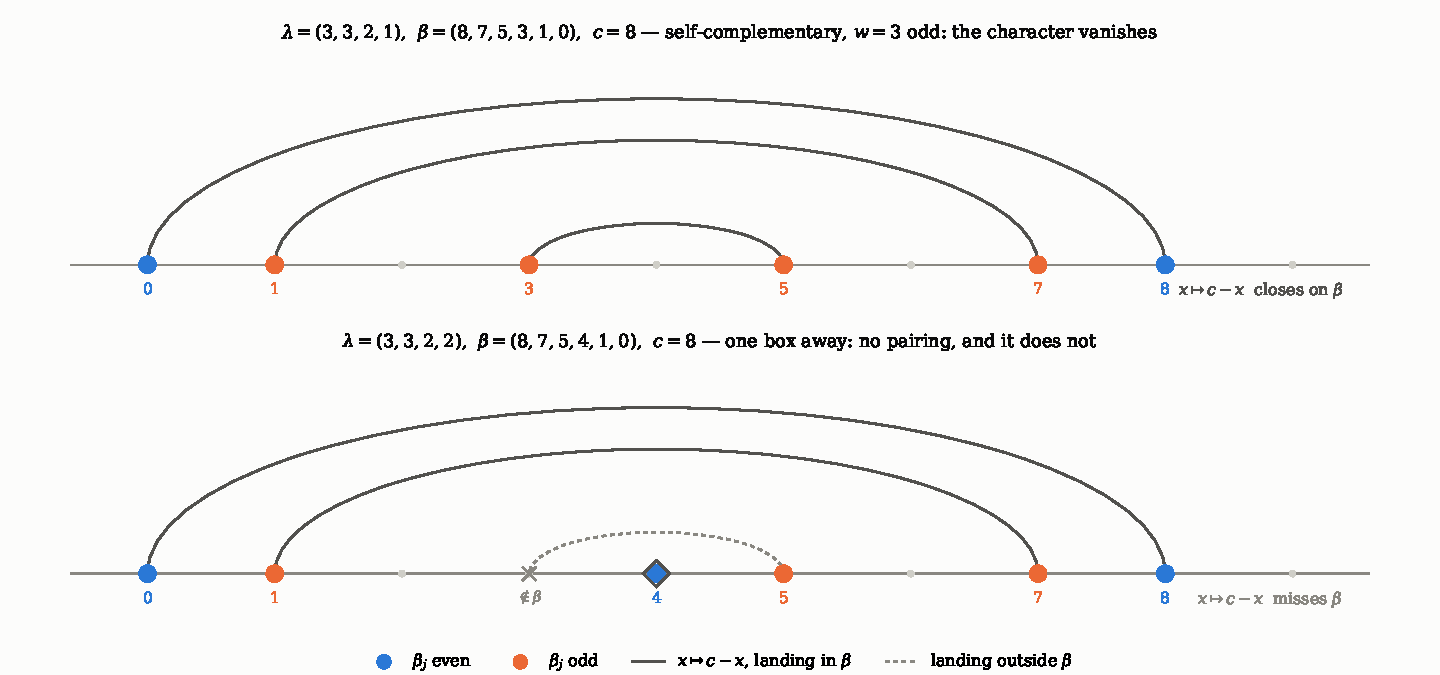
\includegraphics[width=\textwidth]{fig_involution.pdf}
\caption{Why self-complementarity kills the character. Expanding along the two frozen rows leaves
terms indexed by pairs $(e,o)$ with $e\in E$, $o\in O$, and the reflection $x\mapsto c-x$ acts on
them. Above, a self-complementary shape of odd width: every arc lands in $\beta$ and joins entries of
equal parity, because $c$ is even. Below, the same shape with one box moved: the arc $5\mapsto3$
leaves $\beta$, so there is no pairing and nothing cancels. The diamond marks the fixed point of the
reflection, which cannot occur inside an opposite-parity pair --- which is why the involution is
free.}
\label{fig:involution}
\end{figure}

\begin{proof}[Proof of Theorem \ref{thm:r1}]
Put $c_\ast=z+\bar z$ and let $S_n$ be defined by $S_0=0$, $S_1=1$,
$S_{n+1}=c_\ast S_n-S_{n-1}$, so $\deg_{c_\ast}S_n=n-1$ and $S_{-n}=-S_n$; the value $S_{-1}=-1$ is
used whenever $\beta_N=0$. Since $\Phi_A=(x^2-1)(x^2-c_\ast x+1)$, a polynomial $P$ supported on
$\beta$ is divisible by $\Phi_A$ exactly when $P(1)=P(-1)=0$ and $P\equiv0$ modulo $x^2-c_\ast x+1$.
Splitting $P(\pm1)$ by parity and reducing $x^n\equiv S_nx-S_{n-1}$, admissibility becomes the
singularity of the $4\times4$ matrix with rows $[\beta_j\ \mathrm{even}]$,
$[\beta_j\ \mathrm{odd}]$, $S_{\beta_j}$, $S_{\beta_j-1}$. Expanding along the two parity rows and
using d'Ocagne's identity \cite{Doc} for this recurrence,
\begin{equation}\label{eq:docagne}
S_bS_{b'-1}-S_{b'}S_{b-1}=-S_{b-b'},
\end{equation}
each $2\times2$ block collapses to a \emph{single} $S$, indexed by the difference of the two
surviving $\beta$'s. Distinct $S_n$ have distinct degrees in $c_\ast$ and are therefore linearly
independent, so the signed sum vanishes only by exact pairing of equal indices with opposite signs.
The case analysis is finite: $|E|\in\{0,4\}$ is branch (a); $|E|\in\{1,3\}$ leaves three terms whose
indices are the three pairwise differences of a $3$-set and hence always distinct, so no pairing
exists and the value is nonzero; and for $|E|=2$ there are four terms and three perfect matchings,
and one checks the six parity patterns directly. For $E=\{\beta_1,\beta_4\}$ and for
$E=\{\beta_2,\beta_3\}$ exactly one of the three matchings is available and it imposes the single
condition $\beta_1+\beta_4=\beta_2+\beta_3$, which is branch (b); for the four remaining patterns
every one of the three matchings forces two distinct entries of $\beta$ to coincide, so none is
available and the value is nonzero.
\end{proof}

Identity \eqref{eq:docagne} is classical. The collapse it produces is an accident of rank one: two
letters admit a single gap, so $s_{(m,n)}(z,\bar z)=S_{m-n+1}$ depends on that gap alone. There is no
rank-$r$ analogue. One would be a closed form for $s_\mu$ at a reciprocal alphabet for \emph{every}
$\mu$; \cite{CK09} supply that for rectangular shapes and \cite{AB19} for self-complementary ones,
and nobody in general.

For general $r$ we use associates, in Littlewood's sense \cite{Lit50}. On the $\det=-1$ coset $[\nu^{*}]=[\nu]\otimes\det$ gives
$\Psi_r=\sum_\nu\big(m_\nu-m_{\nu^{*}}\big)\chi_{[\nu]}$, so $\Psi_r=0$ if and only if
$m_\nu(\lambda)=m_{\nu^{*}}(\lambda)$ for every $\nu$; equivalently, $V_\lambda|_{O(N)}$ is
$\det$-invariant. A witness is therefore a single $\nu$ with $m_\nu\ne m_{\nu^{*}}$, and it can be
constructed.

Karmakar's \cite[Theorem 4.1]{Kar24} determines the value at the endpoint $z_i=1$, which is an element
of order two: case (A) is branch (a), case (B) is a nonzero dimension, and case (C) leaves an
alternating sum of products of dimensions with no vanishing criterion attached. Branch (b) lives in
that case (C), so the theorem below is not a consequence of it. Nor does case (B) help more as $r$
grows: at $k=1$ it asks that $N-1$ of the $N$ beta numbers share a parity, and the smallest shape
doing so is the staircase $(2r-1,2r-2,\dots,1)$, of size $r(2r-1)$, so on a fixed range of
$|\lambda|$ his nonvanishing case is visible only for small $r$ --- his result is sharpest exactly
where ours is easiest. What connects the endpoint to the
curve at all is rigidity, and rigidity is a statement about our object rather than about the order-two
element: over the ranges of \S\ref{sec:verif} it holds on $\ell(\lambda)\le N/2$ without exception
and fails outside, which is Remark \ref{rem:rankone}.

\begin{proof}[Proof of Theorem \ref{thm:stable}]
Branch (a) cannot occur: with $\ell(\lambda)\le N/2$ at least two trailing parts vanish, so $\beta$
contains two consecutive integers. In Littlewood's range
$m_\nu(\lambda)=\sum_{\beta'\ \mathrm{even}}c^{\lambda}_{\nu\beta'}$, and the term $\beta'=\emptyset$
gives $m_\mu\ge1$ for every $\mu\subseteq\lambda$. Take $\mu$ as follows. If
$\ell(\lambda)<N/2$, take $\mu=\lambda$: then $\ell(\lambda^{*})=N-\ell(\lambda)>\ell(\lambda)$, so
$\lambda^{*}\not\subseteq\lambda$ and $m_{\lambda^{*}}=0\ne m_\lambda$. If $\ell(\lambda)=N/2$ and
$\lambda_{N/2}$ is even, take $\mu=(\lambda_1,\dots,\lambda_{N/2-1})$; then
$\beta'=(\lambda_{N/2})$ is even, $\lambda/\mu$ is a horizontal strip and $m_\mu\ge1$ while
$\ell(\mu)<N/2$, so the previous computation applies to $\mu$. If $\ell(\lambda)=N/2$ and $\lambda$
is not a rectangle, let $j\le N/2-1$ be largest with $\lambda_j>\lambda_{j+1}$ and remove both the
last row and one box from row $j$; then $\beta'=(\lambda_{N/2}+1)$ is even and
$\lambda_j\ge\lambda_{N/2}+1$ keeps $\lambda/\mu$ a horizontal strip. In the remaining case
$\lambda=(k^{\,N/2})$ neither construction is available, and $k$ odd is branch (b) while $k$ even
falls to the second construction.
\end{proof}

\subsection{Outside Littlewood's range}\label{sec:unstable}

For $\ell(\lambda)>N/2$ the restriction rule acquires non-standard labels, and the modification rules
that reduce them are King's \cite{King71}; Koike and Terada \cite{KT87} record that the
type-$D$ specialization sends a universal character to $0$ or to $\pm$ one other, and Fauser, Jarvis,
King and Wybourne observe that beyond the two classical cases \emph{``the general theory, having
infinitely many cases, needs a not yet available formalism''} \cite[\S4]{FJKW05}. Extensions of Littlewood's rule to all parameters do exist for the two classical
cases --- Newell's modification rules \cite{New51}, Sundaram \cite{Sun90} in the symplectic case,
Gavarini's Brauer-algebra proof \cite{Gav99}, and Enright and Willenbring \cite{EW04}, whose Theorem 4
gives the multiplicity as an alternating sum over the Weyl group which in favourable cases collapses
to a difference of two Littlewood coefficients \cite[\S7.11]{EW04}. The route taken here is the dual
one: keep the coefficients universal, which they are in every range, and move the whole
range-dependence into the values, where one lemma disposes of it. On this alphabet no formalism for
the labels is needed at all, and the reason is that the values are not type-$D$ values.

Adding a letter $c$ to an alphabet acts on the ring of symmetric functions by $p_k\mapsto p_k+c^k$;
write $\iota_c$ for that homomorphism. From the generating function of the complete homogeneous
symmetric functions, $h_m(W,c)-c\,h_{m-1}(W,c)=h_m(W)$ for every $m$.

\begin{lemma}[the alphabet is symplectic]\label{lem:AtoSp}
$\iota_{-1}\iota_{1}\,o_\nu=sp_\nu$ for every partition $\nu$, as an identity between Koike--Terada
\emph{universal} characters in $\Lambda$. In particular, for the alphabet
\eqref{eq:psir},
\begin{equation}\label{eq:AtoSp}
o_\nu(A)\;=\;sp_\nu(z_1,\dots,z_r)
\end{equation}
with no hypothesis on $\ell(\nu)$ and with no sign. For $\ell(\nu)>r$ the right-hand side is
that universal character specialized at $r$ variables, not an irreducible $Sp(2r)$ character; it is
the modification rules below that fold it onto one.
\end{lemma}

\begin{proof}
Both steps are Ayyer and Kumari's, and both are the same manipulation: the recurrence turns the
column operations $C_j\to C_j-c\,C_{j-1}$, applied for $j=n,\dots,2$ in that order, into a change of
character type, and operations of that shape leave a determinant unchanged. At $c=1$ they carry the
defining determinant of $o_\nu$ evaluated at $(W,1)$ to that of the odd orthogonal universal
character $so_\nu$ over $W$, which is Koike and Terada's dictionary in the form
$so_\nu(X)=o_\nu(X,\bar X,1,0,0,\dots)$ \cite[(2.13)]{AK25}. At $c=-1$, where the recurrence is
\cite[Proposition 2.1]{AK25} and the operations read $C_j\to C_j+C_{j-1}$, they carry $so_\nu$ to
$sp_\nu$, which is \cite[Lemma 3.2]{AK25}. Composing gives the first statement, and evaluating it on
the reciprocal alphabet $(z_1,\dots,z_r)$ gives \eqref{eq:AtoSp}.
\end{proof}

\noindent Since $\nu'_1=\ell(\nu)$, the trichotomy on $\nu'_1$ against $N/2=r+1$ is a trichotomy on
the length of $\nu$ against the rank of $Sp(2r)$, and the three facts we need are then the classical
symplectic modification rules --- one of the two cases \cite{FJKW05} exempts --- read through
\eqref{eq:AtoSp}: $o_\nu(A)=0$ when $\ell(\nu)=r+1$, the vanishing of a symplectic character one row
past its rank; $o_\nu(A)=\pm o_{\nu^{*}}(A)$ when $\ell(\nu)>r+1$, King's rule folding the label back
onto a dominant one; and the same for non-standard $\nu$, which by Lemma \ref{lem:nonstd} are exactly
the tall ones. The expansion $s_\lambda=\sum_\nu c_\nu o_\nu$, with
$c_\nu=\sum_{\beta'\ \mathrm{even}}c^{\lambda}_{\nu\beta'}$, is an identity of symmetric functions and
holds in every range; specializing it at \eqref{eq:psir} therefore lands every term on
$\{o_\mu(A):\ell(\mu)\le r\}$, which by \eqref{eq:AtoSp} is the set of irreducible characters of
$Sp(2r)$ and so is linearly independent. Figure \ref{fig:reduction} sorts the labels into the four
classes this paragraph describes and computes $o_\nu(A)$ on each, so that the reduction can be seen
to land where it is claimed to. Hence

\begin{figure}[!ht]
\centering
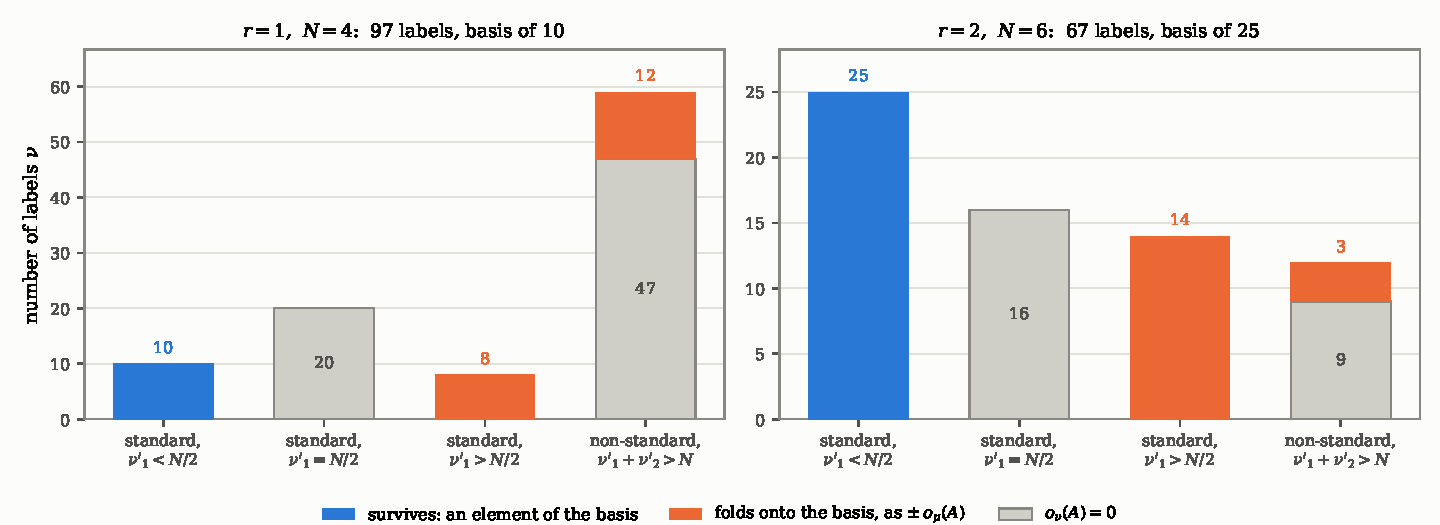
\includegraphics[width=\textwidth]{fig_reduction.pdf}
\caption{The reduction of Lemma \ref{lem:AtoSp}, drawn. Each label $\nu$
occurring in $s_\lambda=\sum_\nu c_\nu o_\nu$ is placed in one of four classes and its value
$o_\nu(A)$ computed. Self-associate labels vanish, every one of them; labels standard with
$\nu'_1>N/2$ fold onto the basis as $\pm o_{\mu}(A)$; non-standard labels either vanish or fold onto
a single basis element with coefficient $\pm1$. By \eqref{eq:AtoSp} these three are the symplectic
modification rules in disguise, the classes being cut by $\ell(\nu)$ against the rank $r$; the figure
was computed before that was noticed, and is left as drawn. Everything lands on the independent
basis $\{o_\mu(A):\ell(\mu)\le r\}$, which is what turns the vanishing into the finite condition
\eqref{eq:Cmu}. The bar heights are label counts over the range each panel was computed on, which is
smaller than the range of the corresponding row of \S\ref{sec:verif}; the classification, not the
count, is what the picture is about.}
\label{fig:reduction}
\end{figure}
\begin{equation}\label{eq:Cmu}
\Psi_r(\lambda)=\sum_{\ell(\mu)\le r}C_\mu(\lambda)\,o_\mu(A),
\qquad
\Psi_r(\lambda)=0\iff C_\mu(\lambda)=0\ \text{for all }\mu,
\end{equation}
where $C_\mu=c_\mu\pm c_{\mu^{*}}+\sum\pm c_\nu$ over the non-standard $\nu$ reducing to $\mu$. The
reduction is carried out in two steps rather than one: most non-standard labels pair with an associate
inside the range, while $21$ of them --- $18$ at $r=1$ and $3$ at $r=2$ --- have no associate in range
and are reduced separately, each landing in the span of the standard values with integer coefficients.

We had computed the three facts before locating them, and record the computation because it is what
the figure below draws: \texttt{sec8\_derivation.sage} checks \eqref{eq:AtoSp} directly for all
$|\nu|\le8$, confirms that the labels of length $r+1$ vanish and that longer ones fold onto the basis
with a sign, and verifies the independence as a rank computation, at $r=1,2,3$. A control that had to
fire: $\iota_1 o_\nu$ and $\iota_{-1}o_\nu$ each agree with $sp_\nu$ only for $\nu=\varnothing$, so
both letters are needed and \eqref{eq:AtoSp} is a statement about the reciprocal pair, not about
either letter alone. \texttt{sec8\_formulas.sage} checks the proof rather than the statement --- the
recurrence at four values of $c$, the two defining determinants against an independent
implementation, and the column operations entry by entry. That last check earned its keep: an earlier
draft of the proof wrote $C_j\to C_j+C_{j-1}$ at $c=1$, the sign \cite[Lemma 3.2]{AK25} uses for its
own step at $c=-1$.

The non-standard labels, which are the whole obstruction here, cannot be small:

\begin{lemma}[non-standard labels are large]\label{lem:nonstd}
Every non-standard $\nu$ occurring in the expansion satisfies $|\nu|\ge N+1=2r+3$. Consequently, if
$|\lambda|\le2r+2$ then no non-standard label is contained in $\lambda$, the last sum in $C_\mu$ is
empty, and $C_\mu(\lambda)=c_\mu(\lambda)\pm c_{\mu^{*}}(\lambda)$ --- with no hypothesis on
$\ell(\lambda)$, hence also outside Littlewood's range.
\end{lemma}

\begin{proof}
Since $c^{\lambda}_{\nu\beta'}=0$ unless $\nu\subseteq\lambda$, only labels with
$\ell(\nu)\le\ell(\lambda)\le N$ occur. Non-standard means $\nu'_1+\nu'_2>N$. Were $\nu$ a single
column we would have $\nu'_2=0$ and hence $\nu'_1=\ell(\nu)>N$, which is excluded; so $\nu'_2\ge1$ and
$|\nu|\ge\nu'_1+\nu'_2>N=2r+2$. A non-standard $\nu$ can therefore contribute only when
$|\lambda|\ge|\nu|\ge2r+3$.
\end{proof}

\noindent Since $\ell(\lambda)>N/2$ forces $|\lambda|\ge r+2$, Lemma \ref{lem:nonstd} settles the
band $r+2\le|\lambda|\le2r+2$ of the unstable range outright: there Littlewood's rule applies
verbatim and the converse follows by the argument of Theorem \ref{thm:stable}. What is left open is
$|\lambda|>2r+2$.


Two exact facts bound the competitors. First $\ell(\mu^{*})=N-\ell(\mu)$, so $\ell(\mu)\le
N-1-\ell(\lambda)$ forces $\mu^{*}\not\subseteq\lambda$ and $c_{\mu^{*}}=0$. Second, a non-standard
$\nu$ has $\nu'_1+\nu'_2>N$ with $\nu'_2\le\nu'_1$, hence $2\ell(\nu)>N$ and $\ell(\nu)\ge r+2$; in
particular no non-standard label fits inside $\lambda$ in Littlewood's range. Call $\mu$
\emph{isolating} for $\lambda$ if exactly one of the labels feeding $C_\mu$ is contained in
$\lambda$; then $C_\mu=\pm c_\nu\ne0$ and $\Psi_r(\lambda)\ne0$. What remains open is one existence
statement.

\begin{proposition}[the isolating witness does not always exist]\label{conj:iso}
At $r=2$ the shape $\lambda=(5,5,2,1)$ has $\Psi_2(\lambda)\ne0$ and is of neither type {\rm(a)} nor
type {\rm(b)}, and no $\mu$ is isolating for it: every $\mu$ whose $C_\mu$ has a nonzero contributor
inside $\lambda$ has exactly two, namely $\mu$ and its associate $\mu^{*}$.
\end{proposition}

We had proposed the isolating witness as the route to Conjecture \ref{conj:crit}, and it does not
reach. The reason is legible in the isolation lemma: it needs $\ell(\mu)\le N-1-\ell(\lambda)$, which
at $\ell(\lambda)=4$ and $N=6$ leaves only one-row $\mu$, and a shape as wide as $(5,5,2,1)$ contains
every associate. Over $r=2$ and $|\lambda|\le14$ there are eleven such shapes, and none at all below
$|\lambda|=13$, which is why the certificate looks sound on small ranges. Conjecture \ref{conj:crit}
itself is untouched --- it asserts that the $C_\mu$ vanish, not that a certificate exists, and it
holds over every shape in the ranges of \S\ref{sec:verif} --- but it is left without a route.

The mechanism does reach a great deal: at $r=2$ and $|\lambda|\le14$, $227$ of the $238$ non-vanishing
unstable shapes carry a proved isolating witness. It also reaches further than fact (ii) allows on
its own --- the true minimum of $\ell(\nu)$ over non-standard $\nu$ with $o_\nu(A)\ne0$ is $5$ there,
against the $r+2=4$ the bound gives. What defeats it is width rather than height: the basis in
\eqref{eq:Cmu} grows with $r$ and the competing labels are constrained to be tall, so we had read
isolation as getting easier with $r$, and along the height axis it does; the residue lives where
$\lambda$ is wide enough to swallow the associates. That reading predicts where the residue is
\emph{not}: at $r=3$ the isolation lemma allows $\ell(\mu)\le7-\ell(\lambda)$, so a shape must be
wider than at $r=2$ before it can swallow every associate, and the same sizes should come out clean.
They do --- over $r=3$ and $|\lambda|\le13$ all $149$ non-vanishing unstable shapes carry a proved
witness and the residue is empty --- which is a control on the explanation rather than a step toward
the conjecture. At $r=1$ the question does not arise, since that case is settled independently by
Theorem \ref{thm:r1}.

The tool one reaches for first does not fit. Saturation, in the honeycomb form of Knutson and Tao
\cite{KT99}, decides when a single Littlewood--Richardson coefficient is positive, and every
competitor feeding $C_\mu$ is positive as soon as its label sits inside $\lambda$. What an isolating
$\mu$ asks for is not positivity but \emph{isolation}: that exactly one of them does. The positivity
is what makes the question hard rather than what answers it, and we know of no tool aimed at the
second question.

\begin{figure}[tb]
\centering
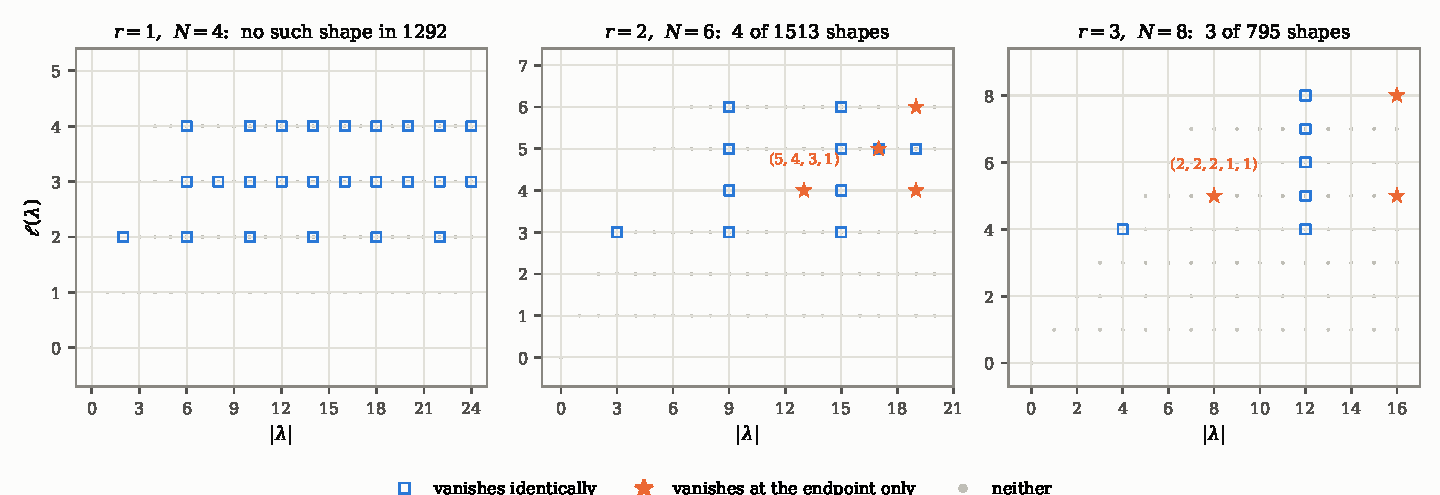
\includegraphics[width=\textwidth]{fig_phase.pdf}
\caption{Where one reciprocal pair stops being typical. Each partition with at most $N$ parts is a
point at $(|\lambda|,\ell(\lambda))$; the class drawn as a star is the one that vanishes at the
endpoint $z_i=1$ without vanishing identically, and it is the whole content of the picture; each
panel names its smallest member and Remark \ref{rem:rankone} lists the rest. The panels cover
$|\lambda|\le24$, $20$ and $16$ respectively. At $r=1$ the class is
empty over all $1292$ shapes in range, because the object there is $\pm$ a genuine character and its
value at the identity is a dimension. From $r=2$ on the object is properly virtual and the class is
not empty. See Remark \ref{rem:rankone}.}
\label{fig:phase}
\end{figure}

\begin{remark}[the rank-one accident, and where the two ranges part]\label{rem:rankone}
At $r=1$ the object is $\pm$ a genuine character, so its value at the identity is a dimension and
$\Psi_1(\lambda)\equiv0$ if and only if $\Psi_1(\lambda)|_{z=1}=0$. At $r\ge2$ the object is properly
virtual and that equivalence fails: $\lambda=(5,4,3,1)$ at $r=2$ has $\Psi_2(\lambda)\ne0$ and
$\Psi_2(\lambda)|_{z_1=z_2=1}=0$. Over the ranges of Figure \ref{fig:phase} the class of such shapes
is empty at $r=1$ across $1292$ partitions; at $r=2$ it consists of the four shapes $(5,4,3,1)$,
$(5,5,4,2,1)$, $(10,5,3,1)$ and $(6,5,4,2,1,1)$, and at $r=3$ of the three shapes $(2,2,2,1,1)$,
$(5,5,4,1,1)$ and $(3,3,3,2,2,1,1,1)$; it is thin, but it is not empty, and one counterexample is all
the equivalence can survive. The surviving implication, exact vanishing $\Rightarrow$ vanishing
at the endpoint, is what makes the endpoint a valid sieve and no more. This is why results computed
at elements of order two \cite{Kar24}, or at variables set to $1$ \cite{Eis07}, bear on the endpoint
and not on the curve, and why Theorem \ref{thm:zeros} is not a corollary of them for $r\ge2$.
\end{remark}

It is worth putting a number on what the endpoint sieve loses, since the qualitative statement is
easy to misread as a small correction. Over the ranges of Figure \ref{fig:phase} the test
$\Psi_r(\lambda)|_{z_i=1}=0$ flags $143$ shapes at $r=1$, $22$ at $r=2$ and $9$ at $r=3$; of those,
$0$, $4$ and $3$ respectively do not vanish identically. So the sieve is exact at one pair, and the
fraction of its verdicts that are spurious grows with the number of pairs --- $0\%$, $18\%$, $33\%$
over these ranges. An endpoint computation is a filter that never misses a genuine zero, and past one
pair it is nothing more than that. The rank-one case at $t=2$, where the sieve happens to be exact
because the object is a genuine character, was treated separately in \cite{Mar26}; the alphabet
\eqref{eq:object} arose there, in a Wilson-line computation on an orbifold, which is why $-1$ appears
as a letter rather than as a choice.

The reason the two ranges of $\ell(\lambda)$ behave so differently is worth separating from the
mechanism that proves it. Littlewood's rule is a statement about which labels $\nu$ can occur, and
$\ell(\lambda)\le N/2$ is exactly the condition under which the non-standard ones cannot fit inside
$\lambda$ at all. Lemma \ref{lem:nonstd} says that the obstruction is governed by $|\lambda|$ as well
as by $\ell(\lambda)$, so the honest picture is not two ranges but a region: the converse is proved
wherever either $\ell(\lambda)\le N/2$ or $|\lambda|\le2r+2$, and outside their union it is open ---
the isolating witness covers most of that region but provably not all of it, by Proposition
\ref{conj:iso}.

%======================================================================
\section{Verification}\label{sec:verif}

Every statement above was checked numerically, by two implementations along different code paths: one
in exact Laurent arithmetic, and one a from-scratch bialternant evaluation written from the
statements alone. The ranges and counts are collected here once.

\begin{center}\footnotesize\setlength{\tabcolsep}{4.2pt}
\begin{tabular}{llrl}
\toprule
statement & range & result & status\\
\midrule
Theorem \ref{thm:main}, sign included & $t\le7$, $|\lambda|\le14,\dots,10$ &
$959$ exact, $476$ zeros, $0$ fail & \stproved\\
Lemma \ref{lem:L1} & $t\le6$ & $454$ nonzero minors & \stproved\\
Lemma \ref{lem:L4} & $t\le7$ & $724/724$ & \stproved\\
Proposition \ref{prop:quotient} & $t\le7$, $|\lambda|\le19$ & $2970/2970$ & \stproved\\
Proposition \ref{rem:lattice} (the concentric locus) & $t\le9$, $|\lambda|\le16$ & $1331/1331$;
$0$ at odd $t$, $43$ at even & \stproved\\
Proposition \ref{rem:sign} (short form of the sign) & $t\le8$, $|\lambda|\le14$ & $1496/1496$;
proof steps $0$ fail & \stproved\\
Proposition \ref{prop:fibrelattice} (the lattice) & $t\le5$, $|\lambda|\le14,12,10,10$ &
$84$, $35$, $20$, $14$ fibres, both ways & \stproved\\
Corollary \ref{cor:fibregf} (the generating function) & same range &
$153/153$; wrong denominator $101$ & \stproved\\
Remark \ref{rem:signsees} (the sign sees the $m_i$) & $t\le4$ &
$107/107$, $43/62$, $26/36$ & \stverif\\
Lemma \ref{lem:single} & $t\le7$, $|\lambda|\le16$ & $2113/2113$ & \stproved\\
Theorem \ref{thm:extra} & $t\le12$, $\lambda_1\le33$ & $119+21$, no others & \stproved\\
Proposition \ref{prop:rect} & $t=2$, $r\le4$, $c\le60$ & $240/240$ & \stproved\\
Corollary \ref{cor:enum} against direct enumeration & $t\le5$ & $14/14$; boxes $16/16$ &
\stproved\\
Proposition \ref{rem:involution} (the runs alternate) & $t=2$, $|\lambda|\le14$, $\le4$ rows &
$4823$ minors; $217$ pairs, $0$ fail & \stproved\\
(D3), (D4) of \S\ref{sec:sharp} & $t\le6$, $|\lambda|\le10$ &
$600$ / $383$ / $200$ of $600$ & \stverif\\
\midrule
\rowcolor{hband} Theorem \ref{thm:zeros}, both directions & $r\le3$, $|\lambda|\le28,26,22$ &
$9961$ shapes, $318$ zeros, $0$ fail & \stverif\\
\rowcolor{hband} \quad branch (a), Thm.~\ref{thm:zeros} & $r\le3$, $|\lambda|\le15$ &
$16/16$ & \stproved\\
\rowcolor{hband} \quad branch (b), Thm.~\ref{thm:zeros} & $r\le3$ & $24/24$ & \stproved\\
\rowcolor{hband} \quad even-width control for (b) & $r\le3$ & $56/56$ nonzero & \stproved\\
\rowcolor{hband} \quad converse at $r=1$, Thm.~\ref{thm:r1} & $\beta_1\le25$ &
$14950$ beta sets, $0$ fail & \stproved\\
\rowcolor{hband} \quad converse, $\ell(\lambda)\le N/2$, Thm.~\ref{thm:stable} & $r\le3$ &
$372/372$ witnesses & \stproved\\
\rowcolor{hband} \quad the isolating witness, Prop.~\ref{conj:iso} & $r=2$, $|\lambda|\le14$ &
$227$ witnesses, $11$ residue & \stproved\\
\rowcolor{hband} \quad the same at $r=3$ & $r=3$, $|\lambda|\le13$ &
$149$ witnesses, $0$ residue & \stproved\\
\midrule
Identity \eqref{eq:compl} & $r\le2$ & $474/474$ & \stproved\\
Identity \eqref{eq:docagne}, and $\deg_{c_\ast}S_n=n-1$ & $b\le31$ & $496/496$; $39/39$ &
\stproved\\
Lemma \ref{lem:AtoSp}, the \S\ref{sec:unstable} reduction & $r\le3$, $|\nu|\le8$ &
identity $0$ fail; folds $0$ fail & \stproved\\
\quad the reduction carried out & $r\le2$ & $236$ labels, $0$ unresolved & \stproved\\
\eqref{eq:Cmu} against the exact object & $r\le2$, both ranges & $184$ shapes, $0$ fail &
\stverif\\
\bottomrule
\end{tabular}
\end{center}

\noindent The shaded block is Theorem \ref{thm:zeros} read from the top down: the two sufficient
branches are proved for every $r$, the converse is proved for one pair and, for every $r$, inside
Littlewood's range, and one line remains --- the converse for $r\ge2$ outside that range and beyond
the band $|\lambda|\le2r+2$ that Lemma \ref{lem:nonstd} settles, which is Conjecture
\ref{conj:crit}. That single \stverif\ line is why the first row of the block is not
labelled \stproved. The row below it records what the certificate we proposed for that line does and
does not do, and it is labelled \stproved\ because Proposition \ref{conj:iso} is a counterexample and
counterexamples are proofs. The rows below the block are the identities and the reduction the section rests
on. In the column, \stproved\ means a proof is given here or cited, and \stverif\ means the
statement is checked exhaustively over the stated range and not proved.

\noindent The (D3), (D4) row is the one that matters most in the first group: the identity holds in
all $600$ cases for \eqref{eq:object} and fails in $217$ and $400$ of them for the two deformed
alphabets, so the test is capable of failing. In the second group the even-width control plays the
same role for Theorem \ref{thm:zeros}: $56$ self-complementary shapes of even width, none of which
vanishes, so the parity hypothesis is doing work rather than decorating. A separate audit rebuilds
all of the second group from the definitions in a single pass, independently of the scripts that
produced them: $3414$ checks, $0$ failures. A second one takes the \emph{displayed formulas} rather
than the counts --- Theorem \ref{thm:LR}, the interval reading \eqref{eq:intervals}, Lemmas
\ref{lem:L2} and \ref{lem:L5}, the splitting \eqref{eq:threestep}, the complementation
\eqref{eq:compl}, d'Ocagne \eqref{eq:docagne} and the scalar caveat \eqref{eq:scalar} --- and
evaluates both sides at numeric points from the definitions, using neither the closed forms of this
paper nor the scripts behind the table: $3297$ evaluations over nine displayed formulas, $0$ failures. The scripts are ancillary to this paper, and so is the
saved output of each one, so every count in the table above can be located in an archived run rather
than taken on trust.

%======================================================================
\section{Open problems}\label{sec:open}

\begin{problem}[the other classical types]\label{prob:types}
Everything above is type $A$. What do $sp_\lambda(\zt,z,\zb)$, $so_\lambda(\zt,z,\zb)$ and
$o_\lambda(\zt,z,\zb)$ do? The root-of-unity factorizations were carried from type $A$ to $B$, $C$,
$D$ by a uniform argument in \cite{AK22} and to the universal characters in \cite{Alb23}; the frozen
rows of the bialternant are the same in every type, so Lemma \ref{lem:L1} and the excess-two count
should survive verbatim, while the collapse, Lemmas \ref{lem:L4} and \ref{lem:L5}, would need
re-deriving once per type. The alphabet \eqref{eq:object} is already a torus element of $O(t+2)$, so
the other types are not the same function at a new point but new objects, and choosing the right ones
is a matter of taste inside a programme we did not build. We have measured, and report it as a
measurement only. Expanding the Koike--Terada universal characters in the Schur basis and evaluating
term by term with Theorem \ref{thm:main}, over $|\lambda|\le12$ for $t\le3$ and $|\lambda|\le10$ for $t=4,5$, the fraction of
$\ell(\lambda)\ge2$ shapes on which the value vanishes is markedly larger for $o_\lambda$ on the
non-identity component than on the identity one --- $83.8\%$ at $t=2$ against $41.8\%$ at $t=3$, and
$58.8\%$ at $t=4$ against $42.1\%$ at $t=5$ --- with $sp_\lambda$ in between and the Schur case
lowest. The effect is real and it tracks the component, which is what one would expect of an
associate cancellation; but it is quantitative and we found no law covering the whole table. A first
attempt at one, that
$o_\lambda$ vanishes for all $\ell(\lambda)\ge2$ when $t$ is even, is false: it was read off a
sample and the systematic sweep refutes it.

The $t=2$ column of that comparison is the one case which does have a law, and it is Lemma
\ref{lem:AtoSp}: there the alphabet is \eqref{eq:psir} at $r=1$, so $o_\nu$ equals $sp_\nu(z)$, a
\emph{rank-one} symplectic character. That vanishes identically for $\ell(\nu)=2$ --- all $36$ such
shapes in range, with no exception --- and folds for $\ell(\nu)>2$, which is why the $t=2$ figure is
the outlier. What remains without a law is odd $t$, where the alphabet is not of the form
\eqref{eq:psir} and the lemma does not apply.

The $sp_\lambda$ column at $t=2$, on the other hand, has an answer, and it explains the asymmetry of
the table rather than adding a row to it. Adjoining the same two letters to a universal
\emph{symplectic} character does not collapse it. Over $|\nu|\le8$,
\begin{equation}\label{eq:spbranch}
sp_\nu(W,1,-1)\;=\;\sum_{\gamma\subseteq\nu}c_{\nu/\gamma}\;sp_\gamma(W),
\end{equation}
where the coefficient depends on $\nu$ and $\gamma$ only through the skew shape $\nu/\gamma$ ---
$247$ coefficients over $74$ distinct skew shapes, with no clash --- and takes only the values $0$
and $\pm1$, vanishing whenever $|\nu/\gamma|$ is odd. That is the shape a branching rule for
universal symplectic functions produces, and such rules are available \cite{JJLW24}. Read against it,
Lemma \ref{lem:AtoSp} says that for $o_\nu$ the corresponding coefficients are concentrated at
$\gamma=\nu$: the two letters collapse the orthogonal character to a single symplectic one, and leave
the symplectic character spread over the whole interval below $\nu$. The asymmetry of the measurement
is that, and not an artefact of the ranges. What we have not done is identify $c_{\nu/\gamma}$, which
\eqref{eq:spbranch} makes a question about skew universal symplectic characters at $(1,-1)$ and
nothing more.

The third column resists the same route, and for a structural reason rather than an accidental one.
What answers the other two is that adjoining a letter is the ring map $p_k\mapsto p_k+c^k$, so
$\iota_{1}$ and $\iota_{-1}$ act on $\Lambda$ and compose. The identity that would bring $so$ into
the picture, $so_\nu(X)=o_\nu(X,\bar X,1,0,\dots)$ of \cite[(2.13)]{AK25}, relates the two on a
\emph{doubled} alphabet instead, and a doubling is not an adjunction: the $\iota$'s do not reach it.
So the $so$ column is not a gap of effort but of mechanism, and we leave it stated as such.
\end{problem}

\begin{problem}[a Verschiebung that sees a reciprocal pair]\label{prob:versch}
The operator $\varphi_t$ has nothing to say about a letter outside a $\zeta$-orbit, which is the
structural reason Theorem \ref{thm:main} is not a corollary of anything in that line, and the reason
our proof descends to the alternant. Is there an operator on universal characters, or a
factorization of $\varphi_t$ through a larger algebra, acting on alphabets of the form (union of
$\zeta$-orbits) $\cup$ (reciprocal pairs)? By \S\ref{sec:sharp} such an operator would decide (D1)
and (D2) at once. The discussion there suggests a quantitative form.

What makes the question well posed rather than vague is that each half already has a formalism, and
they are not the same one. The $\zeta$-orbits are the province of $\varphi_t$, in Albion's
formulation \cite{Alb23}. Alphabets closed under inversion are the province of the universal
symplectic and orthogonal functions, which have vertex operator realizations from which their
branching rules follow \cite{JJLW24}. Our alphabet is one of each, and Lemma \ref{lem:AtoSp} is the
one place where the two meet: there the $\zeta$-orbit is $\{1,-1\}$, small enough that adjoining it
is a pair of letter maps rather than an operator. We know of nothing that acts on both halves at
once, and the question is whether the two formalisms compose.
\end{problem}

\begin{proposition}[the rank is the wrong invariant]\label{conj:rank}
Let $A=\zt\cup B$ with $B$ closed under inversion and disjoint from $\zt$, and let $\rho(B)$ be the
rank of the subgroup of $\CC^{\times}$ generated by $B$. Then $\rho(B)=1$ does not imply that
$s_\lambda(A)$ is a product of characters. At $t=2$ and $B=\{z,z^{-1},z^{2},z^{-2}\}$, which has
$\rho(B)=1$, the value at $\lambda=(2)$ has a root off the unit circle, and so has no such
factorization; the same happens for $B=\{z,z^{-1},z^{3},z^{-3}\}$.
\end{proposition}

\begin{proof}
A product of characters $\chi_k(z)=(z^{k+1}-z^{-k-1})/(z-z^{-1})$ has all of its roots on the unit
circle. For $B=\{z,z^{-1},z^{2},z^{-2}\}$ and $\lambda=(2)$ the value is
$z^{-4}+z^{-3}+z^{-2}+z^{-1}+3+z+z^{2}+z^{3}+z^{4}$, whose roots miss the circle by $0.32$; over
$|\lambda|\le8$ this happens for $17$ of the $62$ nonvanishing shapes, and for
$B=\{z,z^{-1},z^{3},z^{-3}\}$ for $18$. On the same range $B=\{z,z^{-1}\}$ has every root on the
circle without exception, as Theorem \ref{thm:main} requires.
\end{proof}

What the rank does not see is how many free directions $B$ has. A single reciprocal pair is one
direction; $\{z,z^{-1},z^{2},z^{-2}\}$ generates a group of rank one and is two, and the two see each
other. So the invariant to conjecture on is not $\rho(B)$ but the number of independent letters,
and with that reading the statement becomes the one \S\ref{sec:sharp} already makes by other means:

\begin{conjecture}[one free direction]\label{conj:rank2}
$s_\lambda(\zt\cup B)$ is a product of characters for every $\lambda$ if and only if $B$ is a single
reciprocal pair.
\end{conjecture}

The evidence for it is Theorem \ref{thm:main} in one direction and (D1)--(D4) together with
Proposition \ref{conj:rank} in the other: enlarging $B$ destroys the product whether the enlargement
raises the rank or not. We have no proof and no proposed mechanism, and this is precisely the
statement a $\varphi_t$-style argument ought to produce.

One caveat, which the conjecture as stated does not cover. Inversion-closure of $B$ is sufficient in
the evidence above, but it is not necessary for a product. Write $w=-iy$. Then the second block of
the alphabet $\{1,-1,y,-y^{-1}\}$ is not closed under inversion, yet
\begin{equation}\label{eq:scalar}
s_\lambda\big(1,-1,y,-y^{-1}\big)\;=\;i^{\,|\lambda|}\,s_\lambda\big(-i,\,i,\,w,\,w^{-1}\big),
\end{equation}
and the alphabet on the right is. The honest hypothesis is therefore that $A$ be a scalar multiple of
an inversion-closed set. A coset $\zeta\zt$ is itself inversion-closed exactly when
$\zeta^{2}=\pm1$, which is where (D3) does and does not break.

\begin{problem}[the instrument for the second pair]\label{prob:instrument}
Section \ref{sec:zeros} reduces the vanishing at $r\ge2$ to a statement about the coefficients
$C_\mu$ of \eqref{eq:Cmu}, which are signed sums of Littlewood coefficients, and Conjecture
\ref{conj:crit} is what remains --- with no certificate for it, since the one we proposed fails by
Proposition \ref{conj:iso}. Lemma \ref{lem:AtoSp} settles the other half of the reduction --- what
the values $o_\nu(A)$ are --- and settles it symplectically: the two readings of the alphabet agree
because they are the same reading, the orbit Lie algebra of $D_{r+1}$ being $C_r$ rather than the
fixed subalgebra $B_r$. What it does not touch is the coefficients. Kumari and Stokke \cite{KS26}
have given Murnaghan--Nakayama rules for symplectic, orthogonal and orthosymplectic Schur functions;
by Lemma \ref{lem:AtoSp} the relevant one here is the symplectic \cite[Theorem 3.4]{KS26}, not the
even orthogonal \cite[Theorem 3.10]{KS26}. Does the recursion it provides compute $C_\mu$? Their rule
carries a third sum beyond the adding and removing of border strips, and it is the one they single out
as complicated; \cite[Corollary 3.5]{KS26} shows it drops out once $\mu_n+1\ge r$, so it is a
shallow-shape phenomenon. An earlier form of this problem asked whether that sum is what accounts for
the failure of Littlewood's rule outside its range; Lemma \ref{lem:AtoSp} answers that it is not,
since the failure is carried by the symplectic modification rules, which act on the labels and not
inside the recursion. The coefficients are what is left, and whether that recursion computes them is
what we have not attempted.
\end{problem}

\begin{problem}[the extra locus, in general]\label{prob:extralocus}
Does Theorem \ref{thm:extra} have an analogue for $sp$, $so$ and $o$? More generally, for which
specializations of the free variables does the criterion \eqref{eq:AK53} acquire extra solutions, and
can the extra locus always be read off the kernel of the specialization acting on the span of the
universal characters, as Remark \ref{rem:why} suggests? If each type acquires a family indexed by an
order-two element of the residue lattice, the principle is real.

The question needs the free part pinned down, and for a computed reason: the extra family is a
phenomenon of the \emph{minimal} alphabet. Adjoin a second reciprocal pair and it is gone --- over
$t=3,4,5,6$ and $|\lambda|\le14$ the locus is then exactly the $t$-cores, for type $s$ no less than
for $sp$ and $o$, while at one pair type $s$ has the two extras of Theorem \ref{thm:extra} at $t=4$
and one at $t=6$. (We test the second pair at $z_2=z_1^{2}$, a specialization, which can only create
coincidences and not remove them, so a count of zero there is a count of zero.) An analogue for
another type must therefore be sought at \emph{that type's} minimal free part, one letter of each
kind; comparing types across free parts of different sizes measures the free part instead, which is
what our first attempt did.

The kernel is the right thing to look at, but its \emph{presence} does not settle the locus; its
size does. Two free parts of the same size can both collapse the independence and behave quite
differently. On the reciprocal locus $s_\mu(z,\zb)=\chi_{\mu_1-\mu_2}(z)$ retains one grading, and
the extra locus is the single family of Theorem \ref{thm:extra}. Replace the pair by the
$\zeta_2$-orbit $(z,-z)$, where $s_\mu(z,-z)=z^{|\mu|}s_\mu(1,-1)$ retains only $|\mu|$ and a sign,
and over $\ell(\lambda)\le2$ the criterion acquires $28$ further solutions at $t=2$ and $186$ at
$t=8$, in no family we can name. The control is the free pair $(z,w)$, which has no kernel and
returns the $t$-cores and nothing else at every $t\le8$ --- that is \eqref{eq:AK53} itself, so the
control is their theorem rather than a measurement of ours. So the
reciprocal pair is the collapsing specialization of \emph{smallest} kernel, and that, rather than
the mere existence of a kernel, is what makes its extra locus one family.
\end{problem}

\begin{problem}[the fibres, refined by the sign]\label{prob:fibres}
Corollary \ref{cor:fibregf} describes the fibre of the interval triple, and only that. The invariant
is $I_t=(d_1,d_2,d_3,\varepsilon_\lambda)$, and the sign cuts each branch further. Its cut is not
bookkeeping, and it is not idle: by Remark \ref{rem:signsees} the sign sees the $t-2$ directions the
triple does not, from $t=3$ on --- constant in $(m_i)$ at fixed $v$ in all $107$ slots at $t=2$, but
in only $43$ of $62$ at $t=3$ and $26$ of $36$ at $t=4$. What is the restriction of
$\varepsilon_\lambda$ to a branch? The obstruction to reading it off \eqref{eq:fibrelattice} is
visible in \eqref{eq:sign}: $\inv(b_S)$ is a statistic of the whole beta-word, and the lattice
coordinates split that word into two distinguished classes and $t-2$ free letters, so a rule would
have to reassemble what the bijection separates.

Two smaller gaps go with it. The same description for the size-three profile should be the same
bookkeeping with one class of three in place of two of two; we have not written it. The degenerate
profile is a different question, since there the fibre is the whole vanishing locus of $\Phi_t$,
which Corollary \ref{cor:zero} and Proposition \ref{rem:lattice} describe by other means.
\end{problem}

\begin{problem}[a sieving phenomenon that keeps a parameter]\label{prob:sieving}
At $t=2$ Corollary \ref{cor:enum} is a signed count of $\mathrm{SSYT}(\lambda,4)$, and a signed count
of order two is what Stembridge's $q=-1$ phenomenon \cite{Ste94} computes: on a set carrying an
involution, the value at $-1$ counts the fixed points. That is the case $\#C=2$ of the cyclic sieving
phenomenon of Reiner, Stanton and White \cite{RSW04}, whose Theorem 4.3 evaluates the principal
specialization $s_\lambda(1,q,\dots,q^{k-1})$ at a primitive $d$-th root of unity in terms of the
$d$-core and the $d$-quotient of $\lambda$ --- the two invariants that carry Theorem \ref{thm:main}
as well --- and which Lee and Oh \cite{LO22} have since extended to skew shapes. Every evaluation in
that line is at a \emph{number}, as a sieving statement requires: the alphabet there is the geometric
progression $1,q,\dots,q^{k-1}$ specialized at a root of unity, not a plain orbit, and nothing is
left free. Ours is not of that kind --- the reciprocal pair keeps $z$, and \eqref{eq:main} is a
product formula in it. Is there a cyclic action on $\mathrm{SSYT}(\lambda,t+2)$, and a $q$-analogue of
$\Phi_t$, whose value at a $t$-th root of unity counts fixed points refined by $m_{t+1}-m_{t+2}$?
The case $\#C=2$ is where to look first, and there the involution such a statement would need already
exists: \S\ref{sec:enum} assembles it.

The existence half of the question is decidable without exhibiting the action. Alexandersson and
Amini \cite{AA19} give a necessary and sufficient criterion for a cyclic action realizing a given
sieving polynomial to exist: for every $d\mid t$, the value at $\omega^d$ must be
$\sum_{j\mid d}j\,c_j$ with every $c_j$ a nonnegative integer, and the $c_j$ --- the numbers of
orbits of each size --- are then computable by triangularity. Applied to the candidate that the
alphabet itself suggests, $F(q,z)=s_\lambda(1,q,\dots,q^{t-1},z,z^{-1})$, whose $z$-grading is
already the refinement asked for, the criterion is met by almost every graded piece in the ranges we
can reach; but so it is for a deliberately wrong refinement, grading by $m_{t+1}+m_{t+2}$ instead,
which passes at the same rate. At those sizes the criterion does not discriminate, and we report the
attempt as evidence in neither direction.
\end{problem}

One narrower gap is recorded where it arises rather than here, in the same form as the problems
above and with the same meaning --- something we would like to know and have not settled: the
involution of \S\ref{sec:enum} is assembled at $t=2$ and nowhere else, because Proposition
\ref{rem:involution} is a statement about one word and that word is the $t=2$ one. The distinction we
keep throughout is between a \emph{conjecture}, which is a statement we believe and have tested, and
a \emph{problem}, which is not a claim at all.

Taken together the problems say where we think the object stops being ours. The evaluation is
complete and the alphabet is minimal, so what is left is not more of the same: it is whether the two
formalisms that own the two halves of \eqref{eq:object} compose, whether a sieving statement can keep
a variable, and what the coefficients $C_\mu$ do once the certificate we proposed for them is gone.
Of the three, the last is the one the paper needs and the first is the one we would rather see
answered.

\subsection*{Acknowledgements}
This paper exists because Arvind Ayyer asked whether the rank-one case generalizes to arbitrary $t$
with the free variable symbolic. The question was better than the note that prompted it. We thank him
for it, and for the correspondence that followed. Remark \ref{rem:core} exists because Nishu Kumari
asked whether the condition $n_i(\lambda)=0$ could be phrased in terms of the $t$-core; she also
confirmed the reading of \cite[Theorem 5.3]{AK25} in \S\ref{sec:independence}, and it was a pointer
of hers that sent us to \cite[\S3]{AK25}, where Lemma \ref{lem:AtoSp} was waiting; we are grateful
for it. The involution of \S\ref{sec:enum} is assembled from three lemmas of her thesis
\cite{KumariThesis}, and is hers in that sense too.

\subsection*{Code, data and disclosure}
Every computation quoted in this paper is performed by a named script distributed as an ancillary
file, and every number quoted is reproduced by an archived run of one; \S\ref{sec:verif} tabulates
which script answers for which claim. The same scripts and the same archived output are also kept at
\url{https://github.com/karlesmarin/schur-orbit-and-reciprocal-pair}, which is a convenience: the
ancillary files carry everything the paper appeals to. Generative AI (Claude, Anthropic) was used
throughout as a
research assistant --- for literature search, for writing and checking the ancillary code, and on the
prose. The mathematics, and the responsibility for it, are the author's.

%======================================================================
\begin{thebibliography}{AAAA}

\bibitem[Alb23]{Alb23} S.~P.~Albion, \emph{Universal characters twisted by roots of unity},
Algebraic Combinatorics; arXiv:2212.07343.

\bibitem[Alb25]{Alb25} S.~P.~Albion, \emph{Character factorisations, $z$-asymmetric partitions and
plethysm}, arXiv:2501.18520.

\bibitem[AA19]{AA19} P.~Alexandersson and N.~Amini, \emph{The cone of cyclic sieving
phenomena}, Discrete Math. \textbf{342} (2019), no.~6, 1581--1601; arXiv:1804.01447.

\bibitem[AB19]{AB19} A.~Ayyer and R.~E.~Behrend, \emph{Factorization theorems for classical group
characters, with applications to alternating sign matrices and plane partitions}, J. Combin. Theory
Ser.~A \textbf{165} (2019), 78--105; arXiv:1804.04514.

\bibitem[AK22]{AK22} A.~Ayyer and N.~Kumari, \emph{Factorization of classical characters twisted by
roots of unity}, J. Algebra \textbf{609} (2022), 437--483; arXiv:2109.11310.

\bibitem[AK25]{AK25} A.~Ayyer and N.~Kumari, \emph{Further results for classical and universal
characters twisted by roots of unity}, J. Algebraic Combin. \textbf{63} (2025), no.~1;
arXiv:2501.00275.

\bibitem[CK09]{CK09} M.~Ciucu and C.~Krattenthaler, \emph{A factorization theorem for classical
group characters, with applications to plane partitions and rhombus tilings}, in: Advances in
Combinatorial Mathematics, Springer, Berlin, 2009.

\bibitem[GKS90]{GKS90} F.~Garvan, D.~Kim and D.~Stanton, \emph{Cranks and $t$-cores},
Invent. Math. \textbf{101} (1990), no.~1, 1--18.

\bibitem[HI24]{HI24} M.~Hidaka and M.~Itoh, \emph{The Schur polynomials in all primitive $n$th roots
of unity}, J. Combin. Theory Ser.~A; arXiv:2403.10817.

\bibitem[Jan73]{Jantzen} J.~C.~Jantzen, \emph{Darstellungen halbeinfacher algebraischer Gruppen},
Bonner Math. Schriften \textbf{67} (1973).

\bibitem[Kar22]{Kar22} C.~Karmakar, \emph{Character factorizations for representations of
$GL(n,\CC)$}, arXiv:2210.03544.

\bibitem[Kar24]{Kar24} C.~Karmakar, \emph{Character values at elements of order two},
arXiv:2412.17324.

\bibitem[Mar26]{Mar26} C.~Mar\'in, \emph{Schur functions at $(1,-1,t,t^{-1})$: a closed form on the
non-identity component of $O(4)$}, preprint, 2026; \texttt{doi:10.5281/zenodo.21463000}.

\bibitem[JJLW24]{JJLW24} Z.~Jin, N.~Jing, Z.~Li and D.~Wang, \emph{Universal symplectic/orthogonal
functions and general branching rules}, arXiv:2209.00767.

\bibitem[KLP09]{KLP} S.~Kumar, G.~Lusztig and D.~Prasad, \emph{Characters of simply-laced
nonconnected groups versus characters of nonsimply-laced connected groups}, Contemp. Math.
\textbf{478} (2009), 99--101; arXiv:math/0701615.

\bibitem[KT99]{KT99} A.~Knutson and T.~Tao, \emph{The honeycomb model of $GL_n(\CC)$ tensor
products I: proof of the saturation conjecture}, J. Amer. Math. Soc. \textbf{12} (1999), no.~4,
1055--1090.

\bibitem[Kum24]{Kum24} N.~Kumari, \emph{Factorization of classical characters twisted by roots of
unity: II}, J. Pure Appl. Algebra \textbf{228} (2024), no.~11, 107714; arXiv:2212.12477.

\bibitem[KumT]{KumariThesis} N.~Kumari, \emph{Characters of classical groups twisted by roots of
unity}, PhD thesis, Indian Institute of Science, Bangalore, 2023.

\bibitem[Lec09]{Lec09} C.~Lecouvey, \emph{Parabolic Kazhdan--Lusztig polynomials, plethysm and
generalized Hall--Littlewood functions for classical types}, European J. Combin. \textbf{30} (2009),
no.~1, 157--191.

\bibitem[LR34]{LR34} D.~E.~Littlewood and A.~R.~Richardson, \emph{Immanants of some special
matrices}, Q. J. Math. \textbf{os-5} (1934), no.~1, 269--282.

\bibitem[LLT97]{LLT97} A.~Lascoux, B.~Leclerc and J.-Y.~Thibon, \emph{Ribbon tableaux,
Hall--Littlewood functions, quantum affine algebras and unipotent varieties}, J. Math. Phys.
\textbf{38} (1997), no.~2, 1041--1068.

\bibitem[LO22]{LO22} S.-Y.~Lee and Y.-T.~Oh, \emph{Skew Schur polynomials and cyclic sieving
phenomenon}, Electron. J. Combin. \textbf{29} (2022), no.~4, Paper 4.6; arXiv:2112.12394.

\bibitem[Mac95]{Mac95} I.~G.~Macdonald, \emph{Symmetric Functions and Hall Polynomials}, second
edition, Oxford University Press, 1995.

\bibitem[RSW04]{RSW04} V.~Reiner, D.~Stanton and D.~White, \emph{The cyclic sieving phenomenon},
J. Combin. Theory Ser. A \textbf{108} (2004), no.~1, 17--50.

\bibitem[Ste94]{Ste94} J.~R.~Stembridge, \emph{On minuscule representations, plane partitions and
involutions in complex Lie groups}, Duke Math. J. \textbf{73} (1994), no.~2, 469--490.

\bibitem[Oka98]{Oka98} S.~Okada, \emph{Applications of minor summation formulas to
rectangular-shaped representations of classical groups}, J. Algebra \textbf{205} (1998), no.~2,
337--367.

\bibitem[Pra16]{Pra16} D.~Prasad, \emph{A character relationship on $GL_n(\CC)$}, Israel J. Math.
\textbf{211} (2016), no.~1, 257--270.

\bibitem[AF20]{AF20} A.~Ayyer and I.~Fischer, \emph{Bijective proofs of skew Schur polynomial
factorizations}, J. Combin. Theory Ser.~A \textbf{174} (2020), 105241; arXiv:1905.05226.

\bibitem[Eis07]{Eis07} T.~Eisenk\"olbl, \emph{A Schur function identity related to the
$(-1)$-enumeration of self-complementary plane partitions}, J. Combin. Theory Ser.~A \textbf{115}
(2008), 199--212; arXiv:math/0602401.

\bibitem[FJKW05]{FJKW05} B.~Fauser, P.~D.~Jarvis, R.~C.~King and B.~G.~Wybourne, \emph{New branching
rules induced by plethysm}, J. Phys. A \textbf{39} (2006), 2611--2655; arXiv:math-ph/0508034.

\bibitem[Gav99]{Gav99} F.~Gavarini, \emph{A Brauer algebra-theoretic proof of Littlewood's
restriction rules}, J. Algebra \textbf{212} (1999), 240--271.

\bibitem[EW04]{EW04} T.~J.~Enright and J.~F.~Willenbring, \emph{Hilbert series, Howe duality and
branching for classical groups}, Ann. of Math. \textbf{159} (2004), 337--375.

\bibitem[New51]{New51} M.~J.~Newell, \emph{Modification rules for the orthogonal and symplectic
groups}, Proc. Roy. Irish Acad. Sect. A \textbf{54} (1951), 153--163.

\bibitem[Sun90]{Sun90} S.~Sundaram, \emph{Tableaux in the representation theory of the classical Lie
groups}, in \emph{Invariant Theory and Tableaux} (Minneapolis, MN, 1988), IMA Vol. Math. Appl.
\textbf{19}, 191--225, Springer-Verlag, New York, 1990.

\bibitem[IOTZ06]{IOTZ06} M.~Ishikawa, S.~Okada, H.~Tagawa and J.~Zeng, \emph{Generalizations of
Cauchy's determinant and Schur's Pfaffian}, Adv. in Appl. Math. \textbf{36} (2006), 251--287.

\bibitem[Kin71]{King71} R.~C.~King, \emph{Modification rules and products of irreducible
representations of the unitary, orthogonal, and symplectic groups}, J. Math. Phys. \textbf{12}
(1971), 1588--1598.

\bibitem[KT87]{KT87} K.~Koike and I.~Terada, \emph{Young-diagrammatic methods for the representation
theory of the classical groups of type $B_n$, $C_n$, $D_n$}, J. Algebra \textbf{107} (1987),
466--511.

\bibitem[Doc]{Doc} For the name and the surrounding family of identities (Cassini, Catalan,
d'Ocagne, Vajda) see e.g.\ M.~Bunder and J.~Tonien, \emph{Cassini, d'Ocagne and Vajda identities for
$n$-step Fibonacci numbers}, arXiv:2201.06269.

\bibitem[KS26]{KS26} N.~Kumari and A.~Stokke, \emph{Murnaghan--Nakayama rules for symplectic,
orthogonal and orthosymplectic Schur functions}, Discrete Math. \textbf{349} (2026), no.~2;
arXiv:2411.11447.

\bibitem[Kup02]{Kup02} G.~Kuperberg, \emph{Symmetry classes of alternating-sign matrices under one
roof}, Ann. of Math. (2) \textbf{156} (2002), 835--866.

\bibitem[Lit50]{Lit50} D.~E.~Littlewood, \emph{The Theory of Group Characters and Matrix
Representations of Groups}, 2nd ed., Oxford University Press, 1950.

\bibitem[SK23]{SK23} V.~Sathish Kumar, \emph{Flagged skew Schur polynomials twisted by roots of
unity}, arXiv:2306.10289.

\bibitem[Sta86]{Sta86} R.~P.~Stanley, \emph{Symmetries of plane partitions}, J. Combin. Theory
Ser.~A \textbf{43} (1986), 103--113.

\end{thebibliography}

\end{document}
